\documentclass[twoside]{book}

% Packages required by doxygen
\usepackage{calc}
\usepackage{doxygen}
\usepackage{graphicx}
\usepackage[utf8]{inputenc}
\usepackage{makeidx}
\usepackage{multicol}
\usepackage{multirow}
\usepackage{textcomp}
\usepackage[table]{xcolor}

% Font selection
\usepackage[T1]{fontenc}
\usepackage{mathptmx}
\usepackage[scaled=.90]{helvet}
\usepackage{courier}
\usepackage{amssymb}
\usepackage{sectsty}
\renewcommand{\familydefault}{\sfdefault}
\allsectionsfont{%
  \fontseries{bc}\selectfont%
  \color{darkgray}%
}
\renewcommand{\DoxyLabelFont}{%
  \fontseries{bc}\selectfont%
  \color{darkgray}%
}

% Page & text layout
\usepackage{geometry}
\geometry{%
  a4paper,%
  top=2.5cm,%
  bottom=2.5cm,%
  left=2.5cm,%
  right=2.5cm%
}
\tolerance=750
\hfuzz=15pt
\hbadness=750
\setlength{\emergencystretch}{15pt}
\setlength{\parindent}{0cm}
\setlength{\parskip}{0.2cm}
\makeatletter
\renewcommand{\paragraph}{%
  \@startsection{paragraph}{4}{0ex}{-1.0ex}{1.0ex}{%
    \normalfont\normalsize\bfseries\SS@parafont%
  }%
}
\renewcommand{\subparagraph}{%
  \@startsection{subparagraph}{5}{0ex}{-1.0ex}{1.0ex}{%
    \normalfont\normalsize\bfseries\SS@subparafont%
  }%
}
\makeatother

% Headers & footers
\usepackage{fancyhdr}
\pagestyle{fancyplain}
\fancyhead[LE]{\fancyplain{}{\bfseries\thepage}}
\fancyhead[CE]{\fancyplain{}{}}
\fancyhead[RE]{\fancyplain{}{\bfseries\leftmark}}
\fancyhead[LO]{\fancyplain{}{\bfseries\rightmark}}
\fancyhead[CO]{\fancyplain{}{}}
\fancyhead[RO]{\fancyplain{}{\bfseries\thepage}}
\fancyfoot[LE]{\fancyplain{}{}}
\fancyfoot[CE]{\fancyplain{}{}}
\fancyfoot[RE]{\fancyplain{}{\bfseries\scriptsize Generated on Tue Mar 31 2015 18\-:55\-:09 for Inferno by Doxygen }}
\fancyfoot[LO]{\fancyplain{}{\bfseries\scriptsize Generated on Tue Mar 31 2015 18\-:55\-:09 for Inferno by Doxygen }}
\fancyfoot[CO]{\fancyplain{}{}}
\fancyfoot[RO]{\fancyplain{}{}}
\renewcommand{\footrulewidth}{0.4pt}
\renewcommand{\chaptermark}[1]{%
  \markboth{#1}{}%
}
\renewcommand{\sectionmark}[1]{%
  \markright{\thesection\ #1}%
}

% Indices & bibliography
\usepackage{natbib}
\usepackage[titles]{tocloft}
\setcounter{tocdepth}{3}
\setcounter{secnumdepth}{5}
\makeindex

% Hyperlinks (required, but should be loaded last)
\usepackage{ifpdf}
\ifpdf
  \usepackage[pdftex,pagebackref=true]{hyperref}
\else
  \usepackage[ps2pdf,pagebackref=true]{hyperref}
\fi
\hypersetup{%
  colorlinks=true,%
  linkcolor=blue,%
  citecolor=blue,%
  unicode%
}

% Custom commands
\newcommand{\clearemptydoublepage}{%
  \newpage{\pagestyle{empty}\cleardoublepage}%
}


%===== C O N T E N T S =====

\begin{document}

% Titlepage & ToC
\hypersetup{pageanchor=false}
\pagenumbering{roman}
\begin{titlepage}
\vspace*{7cm}
\begin{center}%
{\Large Inferno }\\
\vspace*{1cm}
{\large Generated by Doxygen 1.8.6}\\
\vspace*{0.5cm}
{\small Tue Mar 31 2015 18:55:09}\\
\end{center}
\end{titlepage}
\clearemptydoublepage
\tableofcontents
\clearemptydoublepage
\pagenumbering{arabic}
\hypersetup{pageanchor=true}

%--- Begin generated contents ---
\chapter{Todo List}
\label{todo}
\hypertarget{todo}{}

\begin{DoxyRefList}
\item[\label{todo__todo000002}%
\hypertarget{todo__todo000002}{}%
Global \hyperlink{iutils_8c_ad9b6aaf19fdac7482cc5e8bbb77cb796}{ifast\-\_\-bigpow} (float base, float power)]Let this be a warning to you\-: I have abused the ever loving S\-H\-I\-T out of Hungarian notation up in 'hyah.  
\item[\label{todo__todo000003}%
\hypertarget{todo__todo000003}{}%
Global \hyperlink{iutils_8h_a99799aeb9cb7fb340a3cec124d429764}{ifast\-\_\-sqrt} (float x)]get rid of all those gorram iterations of Newton's method, except we need them for now to get good levels of precision. 

why is it more accurate to just take the magic number hack for rsqrt and inverse it?!? 

I'm sure that rearranging the terms in my Newton's method approximation could kill at least one operation  
\item[\label{todo__todo000001}%
\hypertarget{todo__todo000001}{}%
Global \hyperlink{icoordinates_8h_af824fb9002b49e7348de15d84229e536}{iprint\-\_\-vector} (struct \hyperlink{structivector__t}{ivector\-\_\-t} $\ast$restrict vec)]make it prettier 
\end{DoxyRefList}
\chapter{Data Structure Index}
\section{Data Structures}
Here are the data structures with brief descriptions\-:\begin{DoxyCompactList}
\item\contentsline{section}{\hyperlink{struct__aabb}{\-\_\-aabb} }{\pageref{struct__aabb}}{}
\item\contentsline{section}{\hyperlink{structiabsolutepoint__t}{iabsolutepoint\-\_\-t} }{\pageref{structiabsolutepoint__t}}{}
\item\contentsline{section}{\hyperlink{structicolor__t}{icolor\-\_\-t} }{\pageref{structicolor__t}}{}
\item\contentsline{section}{\hyperlink{structicoloredtriplet__t}{icoloredtriplet\-\_\-t} }{\pageref{structicoloredtriplet__t}}{}
\item\contentsline{section}{\hyperlink{structicolorf__t}{icolorf\-\_\-t} }{\pageref{structicolorf__t}}{}
\item\contentsline{section}{\hyperlink{structievent__handler}{ievent\-\_\-handler} }{\pageref{structievent__handler}}{}
\item\contentsline{section}{\hyperlink{structifrontendstate__t}{ifrontendstate\-\_\-t} }{\pageref{structifrontendstate__t}}{}
\item\contentsline{section}{\hyperlink{structilinked__t}{ilinked\-\_\-t} }{\pageref{structilinked__t}}{}
\item\contentsline{section}{\hyperlink{structilinkedpoint__t}{ilinkedpoint\-\_\-t} }{\pageref{structilinkedpoint__t}}{}
\item\contentsline{section}{\hyperlink{structiobject__t}{iobject\-\_\-t} }{\pageref{structiobject__t}}{}
\item\contentsline{section}{\hyperlink{structipoint__t}{ipoint\-\_\-t} }{\pageref{structipoint__t}}{}
\item\contentsline{section}{\hyperlink{structiregion__t}{iregion\-\_\-t} }{\pageref{structiregion__t}}{}
\item\contentsline{section}{\hyperlink{structitriplet__t}{itriplet\-\_\-t} }{\pageref{structitriplet__t}}{}
\item\contentsline{section}{\hyperlink{structivector__t}{ivector\-\_\-t} }{\pageref{structivector__t}}{}
\end{DoxyCompactList}

\chapter{File Index}
\section{File List}
Here is a list of all files with brief descriptions\-:\begin{DoxyCompactList}
\item\contentsline{section}{src/\hyperlink{error_8c}{error.\-c} }{\pageref{error_8c}}{}
\item\contentsline{section}{src/\hyperlink{error_8h}{error.\-h} }{\pageref{error_8h}}{}
\item\contentsline{section}{src/\hyperlink{icoordinates_8c}{icoordinates.\-c} }{\pageref{icoordinates_8c}}{}
\item\contentsline{section}{src/\hyperlink{icoordinates_8h}{icoordinates.\-h} }{\pageref{icoordinates_8h}}{}
\item\contentsline{section}{src/\hyperlink{igraphics_8c}{igraphics.\-c} }{\pageref{igraphics_8c}}{}
\item\contentsline{section}{src/\hyperlink{igraphics_8h}{igraphics.\-h} }{\pageref{igraphics_8h}}{}
\item\contentsline{section}{src/\hyperlink{inferno_8c}{inferno.\-c} }{\pageref{inferno_8c}}{}
\item\contentsline{section}{src/\hyperlink{inferno_8h}{inferno.\-h} }{\pageref{inferno_8h}}{}
\item\contentsline{section}{src/\hyperlink{iprettyconsole_8h}{iprettyconsole.\-h} }{\pageref{iprettyconsole_8h}}{}
\item\contentsline{section}{src/\hyperlink{iprimitives_8c}{iprimitives.\-c} }{\pageref{iprimitives_8c}}{}
\item\contentsline{section}{src/\hyperlink{iprimitives_8h}{iprimitives.\-h} }{\pageref{iprimitives_8h}}{}
\item\contentsline{section}{src/\hyperlink{isimulation_8c}{isimulation.\-c} }{\pageref{isimulation_8c}}{}
\item\contentsline{section}{src/\hyperlink{isimulation_8h}{isimulation.\-h} }{\pageref{isimulation_8h}}{}
\item\contentsline{section}{src/\hyperlink{itypes_8h}{itypes.\-h} }{\pageref{itypes_8h}}{}
\item\contentsline{section}{src/\hyperlink{iutils_8c}{iutils.\-c} }{\pageref{iutils_8c}}{}
\item\contentsline{section}{src/\hyperlink{iutils_8h}{iutils.\-h} }{\pageref{iutils_8h}}{}
\item\contentsline{section}{src/frontends/\hyperlink{frontend_8c}{frontend.\-c} }{\pageref{frontend_8c}}{}
\item\contentsline{section}{src/frontends/\hyperlink{frontend_8h}{frontend.\-h} }{\pageref{frontend_8h}}{}
\item\contentsline{section}{src/frontends/\hyperlink{frontend__opengl__linux_8c}{frontend\-\_\-opengl\-\_\-linux.\-c} }{\pageref{frontend__opengl__linux_8c}}{}
\item\contentsline{section}{src/frontends/\hyperlink{frontend__opengl__linux_8h}{frontend\-\_\-opengl\-\_\-linux.\-h} }{\pageref{frontend__opengl__linux_8h}}{}
\end{DoxyCompactList}

\chapter{Data Structure Documentation}
\hypertarget{struct__aabb}{\section{\-\_\-aabb Struct Reference}
\label{struct__aabb}\index{\-\_\-aabb@{\-\_\-aabb}}
}


{\ttfamily \#include $<$isimulation.\-h$>$}

\subsection*{Data Fields}
\begin{DoxyCompactItemize}
\item 
float \hyperlink{struct__aabb_a14157451738716a8fb2d71664a01e210}{x}
\item 
float \hyperlink{struct__aabb_a65b0be633481856576e82098405fc9ac}{y}
\item 
float \hyperlink{struct__aabb_af9871006b65a3a58bd13a40e589e25b1}{width}
\item 
float \hyperlink{struct__aabb_a212344ad875dfafbed336f052f2817da}{height}
\end{DoxyCompactItemize}


\subsection{Detailed Description}


Definition at line 7 of file isimulation.\-h.



\subsection{Field Documentation}
\hypertarget{struct__aabb_a212344ad875dfafbed336f052f2817da}{\index{\-\_\-aabb@{\-\_\-aabb}!height@{height}}
\index{height@{height}!_aabb@{\-\_\-aabb}}
\subsubsection[{height}]{\setlength{\rightskip}{0pt plus 5cm}float \-\_\-aabb\-::height}}\label{struct__aabb_a212344ad875dfafbed336f052f2817da}


Definition at line 9 of file isimulation.\-h.

\hypertarget{struct__aabb_af9871006b65a3a58bd13a40e589e25b1}{\index{\-\_\-aabb@{\-\_\-aabb}!width@{width}}
\index{width@{width}!_aabb@{\-\_\-aabb}}
\subsubsection[{width}]{\setlength{\rightskip}{0pt plus 5cm}float \-\_\-aabb\-::width}}\label{struct__aabb_af9871006b65a3a58bd13a40e589e25b1}


Definition at line 9 of file isimulation.\-h.

\hypertarget{struct__aabb_a14157451738716a8fb2d71664a01e210}{\index{\-\_\-aabb@{\-\_\-aabb}!x@{x}}
\index{x@{x}!_aabb@{\-\_\-aabb}}
\subsubsection[{x}]{\setlength{\rightskip}{0pt plus 5cm}float \-\_\-aabb\-::x}}\label{struct__aabb_a14157451738716a8fb2d71664a01e210}


Definition at line 8 of file isimulation.\-h.

\hypertarget{struct__aabb_a65b0be633481856576e82098405fc9ac}{\index{\-\_\-aabb@{\-\_\-aabb}!y@{y}}
\index{y@{y}!_aabb@{\-\_\-aabb}}
\subsubsection[{y}]{\setlength{\rightskip}{0pt plus 5cm}float \-\_\-aabb\-::y}}\label{struct__aabb_a65b0be633481856576e82098405fc9ac}


Definition at line 8 of file isimulation.\-h.



The documentation for this struct was generated from the following file\-:\begin{DoxyCompactItemize}
\item 
src/\hyperlink{isimulation_8h}{isimulation.\-h}\end{DoxyCompactItemize}

\hypertarget{structiabsolutepoint__t}{\section{iabsolutepoint\-\_\-t Struct Reference}
\label{structiabsolutepoint__t}\index{iabsolutepoint\-\_\-t@{iabsolutepoint\-\_\-t}}
}


{\ttfamily \#include $<$icoordinates.\-h$>$}

\subsection*{Data Fields}
\begin{DoxyCompactItemize}
\item 
long double \hyperlink{structiabsolutepoint__t_a7c546cbece73b64e924b982d1647005f}{x}
\item 
long double \hyperlink{structiabsolutepoint__t_a12ea188889c536abe1c6eba40dc62c39}{y}
\item 
\hyperlink{itypes_8h_adde6aaee8457bee49c2a92621fe22b79}{uint8} \hyperlink{structiabsolutepoint__t_a106b4f66e6ffbfcaa4f8c7fc428cc8d0}{z}
\end{DoxyCompactItemize}


\subsection{Detailed Description}


Definition at line 33 of file icoordinates.\-h.



\subsection{Field Documentation}
\hypertarget{structiabsolutepoint__t_a7c546cbece73b64e924b982d1647005f}{\index{iabsolutepoint\-\_\-t@{iabsolutepoint\-\_\-t}!x@{x}}
\index{x@{x}!iabsolutepoint_t@{iabsolutepoint\-\_\-t}}
\subsubsection[{x}]{\setlength{\rightskip}{0pt plus 5cm}long double iabsolutepoint\-\_\-t\-::x}}\label{structiabsolutepoint__t_a7c546cbece73b64e924b982d1647005f}


Definition at line 34 of file icoordinates.\-h.

\hypertarget{structiabsolutepoint__t_a12ea188889c536abe1c6eba40dc62c39}{\index{iabsolutepoint\-\_\-t@{iabsolutepoint\-\_\-t}!y@{y}}
\index{y@{y}!iabsolutepoint_t@{iabsolutepoint\-\_\-t}}
\subsubsection[{y}]{\setlength{\rightskip}{0pt plus 5cm}long double iabsolutepoint\-\_\-t\-::y}}\label{structiabsolutepoint__t_a12ea188889c536abe1c6eba40dc62c39}


Definition at line 35 of file icoordinates.\-h.

\hypertarget{structiabsolutepoint__t_a106b4f66e6ffbfcaa4f8c7fc428cc8d0}{\index{iabsolutepoint\-\_\-t@{iabsolutepoint\-\_\-t}!z@{z}}
\index{z@{z}!iabsolutepoint_t@{iabsolutepoint\-\_\-t}}
\subsubsection[{z}]{\setlength{\rightskip}{0pt plus 5cm}{\bf uint8} iabsolutepoint\-\_\-t\-::z}}\label{structiabsolutepoint__t_a106b4f66e6ffbfcaa4f8c7fc428cc8d0}


Definition at line 36 of file icoordinates.\-h.



The documentation for this struct was generated from the following file\-:\begin{DoxyCompactItemize}
\item 
src/\hyperlink{icoordinates_8h}{icoordinates.\-h}\end{DoxyCompactItemize}

\hypertarget{structicolor__t}{\section{icolor\-\_\-t Struct Reference}
\label{structicolor__t}\index{icolor\-\_\-t@{icolor\-\_\-t}}
}


{\ttfamily \#include $<$iprimitives.\-h$>$}

\subsection*{Data Fields}
\begin{DoxyCompactItemize}
\item 
unsigned char \hyperlink{structicolor__t_af41be99aa200064979c76e29d00d4aff}{r}
\item 
unsigned char \hyperlink{structicolor__t_a3cf0a9335bbc32fc211d22f3ef502110}{g}
\item 
unsigned char \hyperlink{structicolor__t_acb75f6cdb4866b33921bde0c5f9000ce}{b}
\end{DoxyCompactItemize}


\subsection{Detailed Description}


Definition at line 14 of file iprimitives.\-h.



\subsection{Field Documentation}
\hypertarget{structicolor__t_acb75f6cdb4866b33921bde0c5f9000ce}{\index{icolor\-\_\-t@{icolor\-\_\-t}!b@{b}}
\index{b@{b}!icolor_t@{icolor\-\_\-t}}
\subsubsection[{b}]{\setlength{\rightskip}{0pt plus 5cm}unsigned char icolor\-\_\-t\-::b}}\label{structicolor__t_acb75f6cdb4866b33921bde0c5f9000ce}


Definition at line 17 of file iprimitives.\-h.

\hypertarget{structicolor__t_a3cf0a9335bbc32fc211d22f3ef502110}{\index{icolor\-\_\-t@{icolor\-\_\-t}!g@{g}}
\index{g@{g}!icolor_t@{icolor\-\_\-t}}
\subsubsection[{g}]{\setlength{\rightskip}{0pt plus 5cm}unsigned char icolor\-\_\-t\-::g}}\label{structicolor__t_a3cf0a9335bbc32fc211d22f3ef502110}


Definition at line 16 of file iprimitives.\-h.

\hypertarget{structicolor__t_af41be99aa200064979c76e29d00d4aff}{\index{icolor\-\_\-t@{icolor\-\_\-t}!r@{r}}
\index{r@{r}!icolor_t@{icolor\-\_\-t}}
\subsubsection[{r}]{\setlength{\rightskip}{0pt plus 5cm}unsigned char icolor\-\_\-t\-::r}}\label{structicolor__t_af41be99aa200064979c76e29d00d4aff}


Definition at line 15 of file iprimitives.\-h.



The documentation for this struct was generated from the following file\-:\begin{DoxyCompactItemize}
\item 
src/\hyperlink{iprimitives_8h}{iprimitives.\-h}\end{DoxyCompactItemize}

\hypertarget{structicoloredtriplet__t}{\section{icoloredtriplet\-\_\-t Struct Reference}
\label{structicoloredtriplet__t}\index{icoloredtriplet\-\_\-t@{icoloredtriplet\-\_\-t}}
}


{\ttfamily \#include $<$iprimitives.\-h$>$}



Collaboration diagram for icoloredtriplet\-\_\-t\-:\nopagebreak
\begin{figure}[H]
\begin{center}
\leavevmode
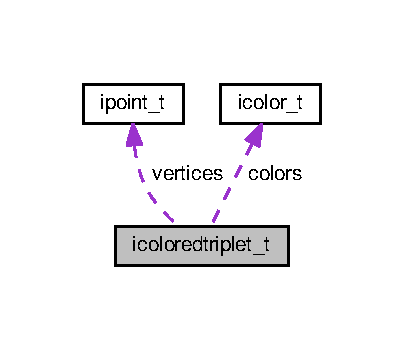
\includegraphics[width=194pt]{structicoloredtriplet__t__coll__graph}
\end{center}
\end{figure}
\subsection*{Data Fields}
\begin{DoxyCompactItemize}
\item 
struct \hyperlink{structipoint__t}{ipoint\-\_\-t} $\ast$ \hyperlink{structicoloredtriplet__t_aa599939c78c387bc80a763f3e3728fee}{vertices} \mbox{[}3\mbox{]}
\item 
struct \hyperlink{structicolor__t}{icolor\-\_\-t} $\ast$ \hyperlink{structicoloredtriplet__t_ac0ba48c5e0ba663bd8c0fb7b3ac2a2a9}{colors} \mbox{[}3\mbox{]}
\end{DoxyCompactItemize}


\subsection{Detailed Description}


Definition at line 28 of file iprimitives.\-h.



\subsection{Field Documentation}
\hypertarget{structicoloredtriplet__t_ac0ba48c5e0ba663bd8c0fb7b3ac2a2a9}{\index{icoloredtriplet\-\_\-t@{icoloredtriplet\-\_\-t}!colors@{colors}}
\index{colors@{colors}!icoloredtriplet_t@{icoloredtriplet\-\_\-t}}
\subsubsection[{colors}]{\setlength{\rightskip}{0pt plus 5cm}struct {\bf icolor\-\_\-t}$\ast$ icoloredtriplet\-\_\-t\-::colors\mbox{[}3\mbox{]}}}\label{structicoloredtriplet__t_ac0ba48c5e0ba663bd8c0fb7b3ac2a2a9}


Definition at line 30 of file iprimitives.\-h.

\hypertarget{structicoloredtriplet__t_aa599939c78c387bc80a763f3e3728fee}{\index{icoloredtriplet\-\_\-t@{icoloredtriplet\-\_\-t}!vertices@{vertices}}
\index{vertices@{vertices}!icoloredtriplet_t@{icoloredtriplet\-\_\-t}}
\subsubsection[{vertices}]{\setlength{\rightskip}{0pt plus 5cm}struct {\bf ipoint\-\_\-t}$\ast$ icoloredtriplet\-\_\-t\-::vertices\mbox{[}3\mbox{]}}}\label{structicoloredtriplet__t_aa599939c78c387bc80a763f3e3728fee}


Definition at line 29 of file iprimitives.\-h.



The documentation for this struct was generated from the following file\-:\begin{DoxyCompactItemize}
\item 
src/\hyperlink{iprimitives_8h}{iprimitives.\-h}\end{DoxyCompactItemize}

\hypertarget{structicolorf__t}{\section{icolorf\-\_\-t Struct Reference}
\label{structicolorf__t}\index{icolorf\-\_\-t@{icolorf\-\_\-t}}
}


{\ttfamily \#include $<$iprimitives.\-h$>$}

\subsection*{Data Fields}
\begin{DoxyCompactItemize}
\item 
float \hyperlink{structicolorf__t_a4b38a1a5c2c96286fd18691bae9fc053}{data} \mbox{[}3\mbox{]}
\end{DoxyCompactItemize}


\subsection{Detailed Description}


Definition at line 20 of file iprimitives.\-h.



\subsection{Field Documentation}
\hypertarget{structicolorf__t_a4b38a1a5c2c96286fd18691bae9fc053}{\index{icolorf\-\_\-t@{icolorf\-\_\-t}!data@{data}}
\index{data@{data}!icolorf_t@{icolorf\-\_\-t}}
\subsubsection[{data}]{\setlength{\rightskip}{0pt plus 5cm}float icolorf\-\_\-t\-::data\mbox{[}3\mbox{]}}}\label{structicolorf__t_a4b38a1a5c2c96286fd18691bae9fc053}


Definition at line 21 of file iprimitives.\-h.



The documentation for this struct was generated from the following file\-:\begin{DoxyCompactItemize}
\item 
src/\hyperlink{iprimitives_8h}{iprimitives.\-h}\end{DoxyCompactItemize}

\hypertarget{structievent__handler}{\section{ievent\-\_\-handler Struct Reference}
\label{structievent__handler}\index{ievent\-\_\-handler@{ievent\-\_\-handler}}
}


{\ttfamily \#include $<$frontend.\-h$>$}

\subsection*{Data Fields}
\begin{DoxyCompactItemize}
\item 
void $\ast$($\ast$ \hyperlink{structievent__handler_a320eaffc01d119279ead9c5ad877c6da}{handler} )(void $\ast$\hyperlink{structievent__handler_ac6b4e6b5b95ada7b0d9985f738ffe1e5}{args}, void $\ast$event)
\item 
void $\ast$ \hyperlink{structievent__handler_ac6b4e6b5b95ada7b0d9985f738ffe1e5}{args}
\item 
unsigned short \hyperlink{structievent__handler_af2766b148965989b8d202b11b9e72f60}{key\-\_\-code}
\end{DoxyCompactItemize}


\subsection{Detailed Description}


Definition at line 13 of file frontend.\-h.



\subsection{Field Documentation}
\hypertarget{structievent__handler_ac6b4e6b5b95ada7b0d9985f738ffe1e5}{\index{ievent\-\_\-handler@{ievent\-\_\-handler}!args@{args}}
\index{args@{args}!ievent_handler@{ievent\-\_\-handler}}
\subsubsection[{args}]{\setlength{\rightskip}{0pt plus 5cm}void$\ast$ ievent\-\_\-handler\-::args}}\label{structievent__handler_ac6b4e6b5b95ada7b0d9985f738ffe1e5}


Definition at line 15 of file frontend.\-h.

\hypertarget{structievent__handler_a320eaffc01d119279ead9c5ad877c6da}{\index{ievent\-\_\-handler@{ievent\-\_\-handler}!handler@{handler}}
\index{handler@{handler}!ievent_handler@{ievent\-\_\-handler}}
\subsubsection[{handler}]{\setlength{\rightskip}{0pt plus 5cm}void$\ast$($\ast$ ievent\-\_\-handler\-::handler)(void $\ast${\bf args}, void $\ast$event)}}\label{structievent__handler_a320eaffc01d119279ead9c5ad877c6da}


Definition at line 14 of file frontend.\-h.

\hypertarget{structievent__handler_af2766b148965989b8d202b11b9e72f60}{\index{ievent\-\_\-handler@{ievent\-\_\-handler}!key\-\_\-code@{key\-\_\-code}}
\index{key\-\_\-code@{key\-\_\-code}!ievent_handler@{ievent\-\_\-handler}}
\subsubsection[{key\-\_\-code}]{\setlength{\rightskip}{0pt plus 5cm}unsigned short ievent\-\_\-handler\-::key\-\_\-code}}\label{structievent__handler_af2766b148965989b8d202b11b9e72f60}


Definition at line 16 of file frontend.\-h.



The documentation for this struct was generated from the following file\-:\begin{DoxyCompactItemize}
\item 
src/frontends/\hyperlink{frontend_8h}{frontend.\-h}\end{DoxyCompactItemize}

\hypertarget{structifrontendstate__t}{\section{ifrontendstate\-\_\-t Struct Reference}
\label{structifrontendstate__t}\index{ifrontendstate\-\_\-t@{ifrontendstate\-\_\-t}}
}


{\ttfamily \#include $<$frontend.\-h$>$}



Collaboration diagram for ifrontendstate\-\_\-t\-:\nopagebreak
\begin{figure}[H]
\begin{center}
\leavevmode
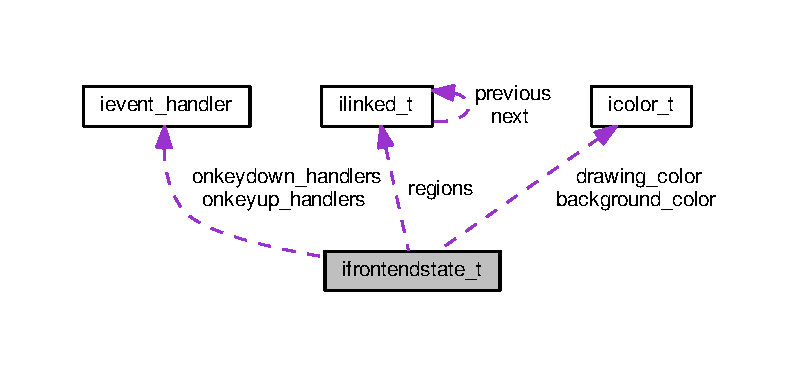
\includegraphics[width=350pt]{structifrontendstate__t__coll__graph}
\end{center}
\end{figure}
\subsection*{Data Fields}
\begin{DoxyCompactItemize}
\item 
struct \hyperlink{structicolor__t}{icolor\-\_\-t} $\ast$ \hyperlink{structifrontendstate__t_afb7c49000e593f77bcb30b1ae4384ded}{background\-\_\-color}
\item 
struct \hyperlink{structicolor__t}{icolor\-\_\-t} $\ast$ \hyperlink{structifrontendstate__t_ac81d750ec8cd1ba1d44e2c0f55bea687}{drawing\-\_\-color}
\item 
char \hyperlink{structifrontendstate__t_aefb96a4cd8758bcd9a3e5b506290adca}{z\-\_\-levels}
\item 
float \hyperlink{structifrontendstate__t_a54ee910059c66c18fa1bb1555d0e61c5}{left}
\item 
float \hyperlink{structifrontendstate__t_a7c304035e472522fb01b3bb85b37eef8}{right}
\item 
float \hyperlink{structifrontendstate__t_adc025993349dceae53dfe235f84fdef2}{bottom}
\item 
float \hyperlink{structifrontendstate__t_afda9cb91a47174c6e95a4888918964f4}{top}
\item 
struct \hyperlink{structievent__handler}{ievent\-\_\-handler} $\ast$ \hyperlink{structifrontendstate__t_ad8fd468eaec37b949af562b39ad20d5a}{onkeydown\-\_\-handlers} \mbox{[}256\mbox{]}
\item 
struct \hyperlink{structievent__handler}{ievent\-\_\-handler} $\ast$ \hyperlink{structifrontendstate__t_a5bb9423c4ba5f86cd8a0d50575031952}{onkeyup\-\_\-handlers} \mbox{[}256\mbox{]}
\item 
struct \hyperlink{structilinked__t}{ilinked\-\_\-t} $\ast$ \hyperlink{structifrontendstate__t_a42ce77321ecea4fde68dd68b7f0f2283}{regions}
\item 
unsigned short \hyperlink{structifrontendstate__t_ad30593dd0b69372008108075c55cfe27}{num\-\_\-regions}
\end{DoxyCompactItemize}


\subsection{Detailed Description}


Definition at line 19 of file frontend.\-h.



\subsection{Field Documentation}
\hypertarget{structifrontendstate__t_afb7c49000e593f77bcb30b1ae4384ded}{\index{ifrontendstate\-\_\-t@{ifrontendstate\-\_\-t}!background\-\_\-color@{background\-\_\-color}}
\index{background\-\_\-color@{background\-\_\-color}!ifrontendstate_t@{ifrontendstate\-\_\-t}}
\subsubsection[{background\-\_\-color}]{\setlength{\rightskip}{0pt plus 5cm}struct {\bf icolor\-\_\-t}$\ast$ ifrontendstate\-\_\-t\-::background\-\_\-color}}\label{structifrontendstate__t_afb7c49000e593f77bcb30b1ae4384ded}


Definition at line 20 of file frontend.\-h.

\hypertarget{structifrontendstate__t_adc025993349dceae53dfe235f84fdef2}{\index{ifrontendstate\-\_\-t@{ifrontendstate\-\_\-t}!bottom@{bottom}}
\index{bottom@{bottom}!ifrontendstate_t@{ifrontendstate\-\_\-t}}
\subsubsection[{bottom}]{\setlength{\rightskip}{0pt plus 5cm}float ifrontendstate\-\_\-t\-::bottom}}\label{structifrontendstate__t_adc025993349dceae53dfe235f84fdef2}


Definition at line 25 of file frontend.\-h.

\hypertarget{structifrontendstate__t_ac81d750ec8cd1ba1d44e2c0f55bea687}{\index{ifrontendstate\-\_\-t@{ifrontendstate\-\_\-t}!drawing\-\_\-color@{drawing\-\_\-color}}
\index{drawing\-\_\-color@{drawing\-\_\-color}!ifrontendstate_t@{ifrontendstate\-\_\-t}}
\subsubsection[{drawing\-\_\-color}]{\setlength{\rightskip}{0pt plus 5cm}struct {\bf icolor\-\_\-t}$\ast$ ifrontendstate\-\_\-t\-::drawing\-\_\-color}}\label{structifrontendstate__t_ac81d750ec8cd1ba1d44e2c0f55bea687}


Definition at line 21 of file frontend.\-h.

\hypertarget{structifrontendstate__t_a54ee910059c66c18fa1bb1555d0e61c5}{\index{ifrontendstate\-\_\-t@{ifrontendstate\-\_\-t}!left@{left}}
\index{left@{left}!ifrontendstate_t@{ifrontendstate\-\_\-t}}
\subsubsection[{left}]{\setlength{\rightskip}{0pt plus 5cm}float ifrontendstate\-\_\-t\-::left}}\label{structifrontendstate__t_a54ee910059c66c18fa1bb1555d0e61c5}


Definition at line 23 of file frontend.\-h.

\hypertarget{structifrontendstate__t_ad30593dd0b69372008108075c55cfe27}{\index{ifrontendstate\-\_\-t@{ifrontendstate\-\_\-t}!num\-\_\-regions@{num\-\_\-regions}}
\index{num\-\_\-regions@{num\-\_\-regions}!ifrontendstate_t@{ifrontendstate\-\_\-t}}
\subsubsection[{num\-\_\-regions}]{\setlength{\rightskip}{0pt plus 5cm}unsigned short ifrontendstate\-\_\-t\-::num\-\_\-regions}}\label{structifrontendstate__t_ad30593dd0b69372008108075c55cfe27}


Definition at line 32 of file frontend.\-h.

\hypertarget{structifrontendstate__t_ad8fd468eaec37b949af562b39ad20d5a}{\index{ifrontendstate\-\_\-t@{ifrontendstate\-\_\-t}!onkeydown\-\_\-handlers@{onkeydown\-\_\-handlers}}
\index{onkeydown\-\_\-handlers@{onkeydown\-\_\-handlers}!ifrontendstate_t@{ifrontendstate\-\_\-t}}
\subsubsection[{onkeydown\-\_\-handlers}]{\setlength{\rightskip}{0pt plus 5cm}struct {\bf ievent\-\_\-handler}$\ast$ ifrontendstate\-\_\-t\-::onkeydown\-\_\-handlers\mbox{[}256\mbox{]}}}\label{structifrontendstate__t_ad8fd468eaec37b949af562b39ad20d5a}


Definition at line 28 of file frontend.\-h.

\hypertarget{structifrontendstate__t_a5bb9423c4ba5f86cd8a0d50575031952}{\index{ifrontendstate\-\_\-t@{ifrontendstate\-\_\-t}!onkeyup\-\_\-handlers@{onkeyup\-\_\-handlers}}
\index{onkeyup\-\_\-handlers@{onkeyup\-\_\-handlers}!ifrontendstate_t@{ifrontendstate\-\_\-t}}
\subsubsection[{onkeyup\-\_\-handlers}]{\setlength{\rightskip}{0pt plus 5cm}struct {\bf ievent\-\_\-handler}$\ast$ ifrontendstate\-\_\-t\-::onkeyup\-\_\-handlers\mbox{[}256\mbox{]}}}\label{structifrontendstate__t_a5bb9423c4ba5f86cd8a0d50575031952}


Definition at line 29 of file frontend.\-h.

\hypertarget{structifrontendstate__t_a42ce77321ecea4fde68dd68b7f0f2283}{\index{ifrontendstate\-\_\-t@{ifrontendstate\-\_\-t}!regions@{regions}}
\index{regions@{regions}!ifrontendstate_t@{ifrontendstate\-\_\-t}}
\subsubsection[{regions}]{\setlength{\rightskip}{0pt plus 5cm}struct {\bf ilinked\-\_\-t}$\ast$ ifrontendstate\-\_\-t\-::regions}}\label{structifrontendstate__t_a42ce77321ecea4fde68dd68b7f0f2283}


Definition at line 31 of file frontend.\-h.

\hypertarget{structifrontendstate__t_a7c304035e472522fb01b3bb85b37eef8}{\index{ifrontendstate\-\_\-t@{ifrontendstate\-\_\-t}!right@{right}}
\index{right@{right}!ifrontendstate_t@{ifrontendstate\-\_\-t}}
\subsubsection[{right}]{\setlength{\rightskip}{0pt plus 5cm}float ifrontendstate\-\_\-t\-::right}}\label{structifrontendstate__t_a7c304035e472522fb01b3bb85b37eef8}


Definition at line 24 of file frontend.\-h.

\hypertarget{structifrontendstate__t_afda9cb91a47174c6e95a4888918964f4}{\index{ifrontendstate\-\_\-t@{ifrontendstate\-\_\-t}!top@{top}}
\index{top@{top}!ifrontendstate_t@{ifrontendstate\-\_\-t}}
\subsubsection[{top}]{\setlength{\rightskip}{0pt plus 5cm}float ifrontendstate\-\_\-t\-::top}}\label{structifrontendstate__t_afda9cb91a47174c6e95a4888918964f4}


Definition at line 26 of file frontend.\-h.

\hypertarget{structifrontendstate__t_aefb96a4cd8758bcd9a3e5b506290adca}{\index{ifrontendstate\-\_\-t@{ifrontendstate\-\_\-t}!z\-\_\-levels@{z\-\_\-levels}}
\index{z\-\_\-levels@{z\-\_\-levels}!ifrontendstate_t@{ifrontendstate\-\_\-t}}
\subsubsection[{z\-\_\-levels}]{\setlength{\rightskip}{0pt plus 5cm}char ifrontendstate\-\_\-t\-::z\-\_\-levels}}\label{structifrontendstate__t_aefb96a4cd8758bcd9a3e5b506290adca}


Definition at line 22 of file frontend.\-h.



The documentation for this struct was generated from the following file\-:\begin{DoxyCompactItemize}
\item 
src/frontends/\hyperlink{frontend_8h}{frontend.\-h}\end{DoxyCompactItemize}

\hypertarget{structilinked__t}{\section{ilinked\-\_\-t Struct Reference}
\label{structilinked__t}\index{ilinked\-\_\-t@{ilinked\-\_\-t}}
}


{\ttfamily \#include $<$iutils.\-h$>$}



Collaboration diagram for ilinked\-\_\-t\-:\nopagebreak
\begin{figure}[H]
\begin{center}
\leavevmode
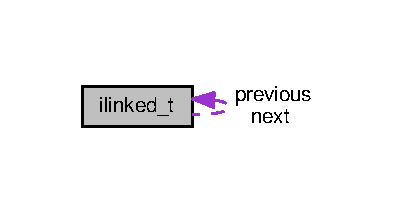
\includegraphics[width=190pt]{structilinked__t__coll__graph}
\end{center}
\end{figure}
\subsection*{Data Fields}
\begin{DoxyCompactItemize}
\item 
struct \hyperlink{structilinked__t}{ilinked\-\_\-t} $\ast$ \hyperlink{structilinked__t_a6bace3c90bc1b272be7506fe4d259a71}{previous}
\item 
void $\ast$ \hyperlink{structilinked__t_ac285ea385953cbd5a332b2cbab39b62b}{data}
\item 
struct \hyperlink{structilinked__t}{ilinked\-\_\-t} $\ast$ \hyperlink{structilinked__t_ad3f173c464d58934b12da4eca2ff83f8}{next}
\end{DoxyCompactItemize}


\subsection{Detailed Description}


Definition at line 10 of file iutils.\-h.



\subsection{Field Documentation}
\hypertarget{structilinked__t_ac285ea385953cbd5a332b2cbab39b62b}{\index{ilinked\-\_\-t@{ilinked\-\_\-t}!data@{data}}
\index{data@{data}!ilinked_t@{ilinked\-\_\-t}}
\subsubsection[{data}]{\setlength{\rightskip}{0pt plus 5cm}void$\ast$ ilinked\-\_\-t\-::data}}\label{structilinked__t_ac285ea385953cbd5a332b2cbab39b62b}


Definition at line 12 of file iutils.\-h.

\hypertarget{structilinked__t_ad3f173c464d58934b12da4eca2ff83f8}{\index{ilinked\-\_\-t@{ilinked\-\_\-t}!next@{next}}
\index{next@{next}!ilinked_t@{ilinked\-\_\-t}}
\subsubsection[{next}]{\setlength{\rightskip}{0pt plus 5cm}struct {\bf ilinked\-\_\-t}$\ast$ ilinked\-\_\-t\-::next}}\label{structilinked__t_ad3f173c464d58934b12da4eca2ff83f8}


Definition at line 13 of file iutils.\-h.

\hypertarget{structilinked__t_a6bace3c90bc1b272be7506fe4d259a71}{\index{ilinked\-\_\-t@{ilinked\-\_\-t}!previous@{previous}}
\index{previous@{previous}!ilinked_t@{ilinked\-\_\-t}}
\subsubsection[{previous}]{\setlength{\rightskip}{0pt plus 5cm}struct {\bf ilinked\-\_\-t}$\ast$ ilinked\-\_\-t\-::previous}}\label{structilinked__t_a6bace3c90bc1b272be7506fe4d259a71}


Definition at line 11 of file iutils.\-h.



The documentation for this struct was generated from the following file\-:\begin{DoxyCompactItemize}
\item 
src/\hyperlink{iutils_8h}{iutils.\-h}\end{DoxyCompactItemize}

\hypertarget{structilinkedpoint__t}{\section{ilinkedpoint\-\_\-t Struct Reference}
\label{structilinkedpoint__t}\index{ilinkedpoint\-\_\-t@{ilinkedpoint\-\_\-t}}
}


{\ttfamily \#include $<$icoordinates.\-h$>$}



Collaboration diagram for ilinkedpoint\-\_\-t\-:\nopagebreak
\begin{figure}[H]
\begin{center}
\leavevmode
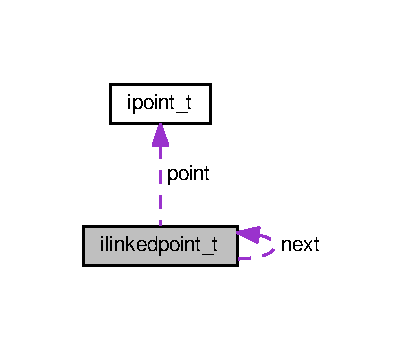
\includegraphics[width=194pt]{structilinkedpoint__t__coll__graph}
\end{center}
\end{figure}
\subsection*{Data Fields}
\begin{DoxyCompactItemize}
\item 
struct \hyperlink{structipoint__t}{ipoint\-\_\-t} $\ast$ \hyperlink{structilinkedpoint__t_ad679b26e2151ec3a4ad7b062679fd3c3}{point}
\item 
struct \hyperlink{structilinkedpoint__t}{ilinkedpoint\-\_\-t} $\ast$ \hyperlink{structilinkedpoint__t_a3af3bf37f168b5b11fce11262286d6c4}{next}
\end{DoxyCompactItemize}


\subsection{Detailed Description}


Definition at line 39 of file icoordinates.\-h.



\subsection{Field Documentation}
\hypertarget{structilinkedpoint__t_a3af3bf37f168b5b11fce11262286d6c4}{\index{ilinkedpoint\-\_\-t@{ilinkedpoint\-\_\-t}!next@{next}}
\index{next@{next}!ilinkedpoint_t@{ilinkedpoint\-\_\-t}}
\subsubsection[{next}]{\setlength{\rightskip}{0pt plus 5cm}struct {\bf ilinkedpoint\-\_\-t}$\ast$ ilinkedpoint\-\_\-t\-::next}}\label{structilinkedpoint__t_a3af3bf37f168b5b11fce11262286d6c4}


Definition at line 41 of file icoordinates.\-h.

\hypertarget{structilinkedpoint__t_ad679b26e2151ec3a4ad7b062679fd3c3}{\index{ilinkedpoint\-\_\-t@{ilinkedpoint\-\_\-t}!point@{point}}
\index{point@{point}!ilinkedpoint_t@{ilinkedpoint\-\_\-t}}
\subsubsection[{point}]{\setlength{\rightskip}{0pt plus 5cm}struct {\bf ipoint\-\_\-t}$\ast$ ilinkedpoint\-\_\-t\-::point}}\label{structilinkedpoint__t_ad679b26e2151ec3a4ad7b062679fd3c3}


Definition at line 40 of file icoordinates.\-h.



The documentation for this struct was generated from the following file\-:\begin{DoxyCompactItemize}
\item 
src/\hyperlink{icoordinates_8h}{icoordinates.\-h}\end{DoxyCompactItemize}

\hypertarget{structiobject__t}{\section{iobject\-\_\-t Struct Reference}
\label{structiobject__t}\index{iobject\-\_\-t@{iobject\-\_\-t}}
}


{\ttfamily \#include $<$iprimitives.\-h$>$}



Collaboration diagram for iobject\-\_\-t\-:\nopagebreak
\begin{figure}[H]
\begin{center}
\leavevmode
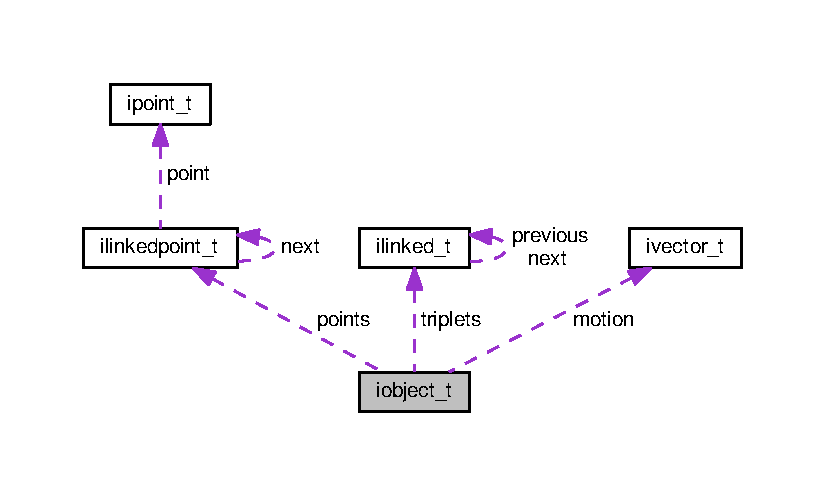
\includegraphics[width=350pt]{structiobject__t__coll__graph}
\end{center}
\end{figure}
\subsection*{Data Fields}
\begin{DoxyCompactItemize}
\item 
struct \hyperlink{structilinked__t}{ilinked\-\_\-t} $\ast$ \hyperlink{structiobject__t_ae5c7b9d49120fc7003f01fcf7055b425}{triplets}
\item 
int \hyperlink{structiobject__t_aa2cbae39b6848c1036afebae90a0bd8c}{num\-\_\-triplets}
\item 
struct \hyperlink{structilinkedpoint__t}{ilinkedpoint\-\_\-t} $\ast$ \hyperlink{structiobject__t_aaf44cb85cf392a8ac7e30ab6971be2ad}{points}
\item 
int \hyperlink{structiobject__t_a281441e3843f4753cd3893f750e78773}{num\-\_\-points}
\item 
struct \hyperlink{structivector__t}{ivector\-\_\-t} $\ast$ \hyperlink{structiobject__t_a95a087e73bb5b8d3fa5e2afd61a3a3c5}{motion}
\item 
int($\ast$ \hyperlink{structiobject__t_ae36734213d8eb5491df4b99193307450}{step} )(void $\ast$)
\end{DoxyCompactItemize}


\subsection{Detailed Description}


Definition at line 45 of file iprimitives.\-h.



\subsection{Field Documentation}
\hypertarget{structiobject__t_a95a087e73bb5b8d3fa5e2afd61a3a3c5}{\index{iobject\-\_\-t@{iobject\-\_\-t}!motion@{motion}}
\index{motion@{motion}!iobject_t@{iobject\-\_\-t}}
\subsubsection[{motion}]{\setlength{\rightskip}{0pt plus 5cm}struct {\bf ivector\-\_\-t}$\ast$ iobject\-\_\-t\-::motion}}\label{structiobject__t_a95a087e73bb5b8d3fa5e2afd61a3a3c5}


Definition at line 50 of file iprimitives.\-h.

\hypertarget{structiobject__t_a281441e3843f4753cd3893f750e78773}{\index{iobject\-\_\-t@{iobject\-\_\-t}!num\-\_\-points@{num\-\_\-points}}
\index{num\-\_\-points@{num\-\_\-points}!iobject_t@{iobject\-\_\-t}}
\subsubsection[{num\-\_\-points}]{\setlength{\rightskip}{0pt plus 5cm}int iobject\-\_\-t\-::num\-\_\-points}}\label{structiobject__t_a281441e3843f4753cd3893f750e78773}


Definition at line 49 of file iprimitives.\-h.

\hypertarget{structiobject__t_aa2cbae39b6848c1036afebae90a0bd8c}{\index{iobject\-\_\-t@{iobject\-\_\-t}!num\-\_\-triplets@{num\-\_\-triplets}}
\index{num\-\_\-triplets@{num\-\_\-triplets}!iobject_t@{iobject\-\_\-t}}
\subsubsection[{num\-\_\-triplets}]{\setlength{\rightskip}{0pt plus 5cm}int iobject\-\_\-t\-::num\-\_\-triplets}}\label{structiobject__t_aa2cbae39b6848c1036afebae90a0bd8c}


Definition at line 47 of file iprimitives.\-h.

\hypertarget{structiobject__t_aaf44cb85cf392a8ac7e30ab6971be2ad}{\index{iobject\-\_\-t@{iobject\-\_\-t}!points@{points}}
\index{points@{points}!iobject_t@{iobject\-\_\-t}}
\subsubsection[{points}]{\setlength{\rightskip}{0pt plus 5cm}struct {\bf ilinkedpoint\-\_\-t}$\ast$ iobject\-\_\-t\-::points}}\label{structiobject__t_aaf44cb85cf392a8ac7e30ab6971be2ad}


Definition at line 48 of file iprimitives.\-h.

\hypertarget{structiobject__t_ae36734213d8eb5491df4b99193307450}{\index{iobject\-\_\-t@{iobject\-\_\-t}!step@{step}}
\index{step@{step}!iobject_t@{iobject\-\_\-t}}
\subsubsection[{step}]{\setlength{\rightskip}{0pt plus 5cm}int($\ast$ iobject\-\_\-t\-::step)(void $\ast$)}}\label{structiobject__t_ae36734213d8eb5491df4b99193307450}


Definition at line 51 of file iprimitives.\-h.

\hypertarget{structiobject__t_ae5c7b9d49120fc7003f01fcf7055b425}{\index{iobject\-\_\-t@{iobject\-\_\-t}!triplets@{triplets}}
\index{triplets@{triplets}!iobject_t@{iobject\-\_\-t}}
\subsubsection[{triplets}]{\setlength{\rightskip}{0pt plus 5cm}struct {\bf ilinked\-\_\-t}$\ast$ iobject\-\_\-t\-::triplets}}\label{structiobject__t_ae5c7b9d49120fc7003f01fcf7055b425}


Definition at line 46 of file iprimitives.\-h.



The documentation for this struct was generated from the following file\-:\begin{DoxyCompactItemize}
\item 
src/\hyperlink{iprimitives_8h}{iprimitives.\-h}\end{DoxyCompactItemize}

\hypertarget{structipoint__t}{\section{ipoint\-\_\-t Struct Reference}
\label{structipoint__t}\index{ipoint\-\_\-t@{ipoint\-\_\-t}}
}


{\ttfamily \#include $<$icoordinates.\-h$>$}

\subsection*{Data Fields}
\begin{DoxyCompactItemize}
\item 
float \hyperlink{structipoint__t_a345608e139b0709cc281139e3ed6328d}{x}
\item 
float \hyperlink{structipoint__t_a88ca543f1508de060b4738cfebb51b04}{y}
\item 
\hyperlink{itypes_8h_adde6aaee8457bee49c2a92621fe22b79}{uint8} \hyperlink{structipoint__t_ad1680bc07190dabf544e86824b82e44b}{z}
\item 
unsigned short \hyperlink{structipoint__t_a92092dc10d022e8cbeea97795e16f55b}{region}
\end{DoxyCompactItemize}


\subsection{Detailed Description}


Definition at line 26 of file icoordinates.\-h.



\subsection{Field Documentation}
\hypertarget{structipoint__t_a92092dc10d022e8cbeea97795e16f55b}{\index{ipoint\-\_\-t@{ipoint\-\_\-t}!region@{region}}
\index{region@{region}!ipoint_t@{ipoint\-\_\-t}}
\subsubsection[{region}]{\setlength{\rightskip}{0pt plus 5cm}unsigned short ipoint\-\_\-t\-::region}}\label{structipoint__t_a92092dc10d022e8cbeea97795e16f55b}


Definition at line 30 of file icoordinates.\-h.

\hypertarget{structipoint__t_a345608e139b0709cc281139e3ed6328d}{\index{ipoint\-\_\-t@{ipoint\-\_\-t}!x@{x}}
\index{x@{x}!ipoint_t@{ipoint\-\_\-t}}
\subsubsection[{x}]{\setlength{\rightskip}{0pt plus 5cm}float ipoint\-\_\-t\-::x}}\label{structipoint__t_a345608e139b0709cc281139e3ed6328d}


Definition at line 27 of file icoordinates.\-h.

\hypertarget{structipoint__t_a88ca543f1508de060b4738cfebb51b04}{\index{ipoint\-\_\-t@{ipoint\-\_\-t}!y@{y}}
\index{y@{y}!ipoint_t@{ipoint\-\_\-t}}
\subsubsection[{y}]{\setlength{\rightskip}{0pt plus 5cm}float ipoint\-\_\-t\-::y}}\label{structipoint__t_a88ca543f1508de060b4738cfebb51b04}


Definition at line 28 of file icoordinates.\-h.

\hypertarget{structipoint__t_ad1680bc07190dabf544e86824b82e44b}{\index{ipoint\-\_\-t@{ipoint\-\_\-t}!z@{z}}
\index{z@{z}!ipoint_t@{ipoint\-\_\-t}}
\subsubsection[{z}]{\setlength{\rightskip}{0pt plus 5cm}{\bf uint8} ipoint\-\_\-t\-::z}}\label{structipoint__t_ad1680bc07190dabf544e86824b82e44b}


Definition at line 29 of file icoordinates.\-h.



The documentation for this struct was generated from the following file\-:\begin{DoxyCompactItemize}
\item 
src/\hyperlink{icoordinates_8h}{icoordinates.\-h}\end{DoxyCompactItemize}

\hypertarget{structiregion__t}{\section{iregion\-\_\-t Struct Reference}
\label{structiregion__t}\index{iregion\-\_\-t@{iregion\-\_\-t}}
}


{\ttfamily \#include $<$icoordinates.\-h$>$}

\subsection*{Data Fields}
\begin{DoxyCompactItemize}
\item 
unsigned short \hyperlink{structiregion__t_a09ef2d2779286827357a7c3290e65d9a}{id}
\item 
int \hyperlink{structiregion__t_a244884f21e4d054538530e389755ac3e}{x}
\item 
int \hyperlink{structiregion__t_a8b975f923a92e3969b4aec3d935af310}{y}
\item 
\hyperlink{itypes_8h_a1134b580f8da4de94ca6b1de4d37975e}{uint32} \hyperlink{structiregion__t_abcafee0857bd757384813e53ddf879d9}{width}
\item 
\hyperlink{itypes_8h_a1134b580f8da4de94ca6b1de4d37975e}{uint32} \hyperlink{structiregion__t_ac7c841eeb48c334a9a7182480855d251}{height}
\end{DoxyCompactItemize}


\subsection{Detailed Description}


Definition at line 18 of file icoordinates.\-h.



\subsection{Field Documentation}
\hypertarget{structiregion__t_ac7c841eeb48c334a9a7182480855d251}{\index{iregion\-\_\-t@{iregion\-\_\-t}!height@{height}}
\index{height@{height}!iregion_t@{iregion\-\_\-t}}
\subsubsection[{height}]{\setlength{\rightskip}{0pt plus 5cm}{\bf uint32} iregion\-\_\-t\-::height}}\label{structiregion__t_ac7c841eeb48c334a9a7182480855d251}


Definition at line 23 of file icoordinates.\-h.

\hypertarget{structiregion__t_a09ef2d2779286827357a7c3290e65d9a}{\index{iregion\-\_\-t@{iregion\-\_\-t}!id@{id}}
\index{id@{id}!iregion_t@{iregion\-\_\-t}}
\subsubsection[{id}]{\setlength{\rightskip}{0pt plus 5cm}unsigned short iregion\-\_\-t\-::id}}\label{structiregion__t_a09ef2d2779286827357a7c3290e65d9a}


Definition at line 19 of file icoordinates.\-h.

\hypertarget{structiregion__t_abcafee0857bd757384813e53ddf879d9}{\index{iregion\-\_\-t@{iregion\-\_\-t}!width@{width}}
\index{width@{width}!iregion_t@{iregion\-\_\-t}}
\subsubsection[{width}]{\setlength{\rightskip}{0pt plus 5cm}{\bf uint32} iregion\-\_\-t\-::width}}\label{structiregion__t_abcafee0857bd757384813e53ddf879d9}


Definition at line 22 of file icoordinates.\-h.

\hypertarget{structiregion__t_a244884f21e4d054538530e389755ac3e}{\index{iregion\-\_\-t@{iregion\-\_\-t}!x@{x}}
\index{x@{x}!iregion_t@{iregion\-\_\-t}}
\subsubsection[{x}]{\setlength{\rightskip}{0pt plus 5cm}int iregion\-\_\-t\-::x}}\label{structiregion__t_a244884f21e4d054538530e389755ac3e}


Definition at line 20 of file icoordinates.\-h.

\hypertarget{structiregion__t_a8b975f923a92e3969b4aec3d935af310}{\index{iregion\-\_\-t@{iregion\-\_\-t}!y@{y}}
\index{y@{y}!iregion_t@{iregion\-\_\-t}}
\subsubsection[{y}]{\setlength{\rightskip}{0pt plus 5cm}int iregion\-\_\-t\-::y}}\label{structiregion__t_a8b975f923a92e3969b4aec3d935af310}


Definition at line 21 of file icoordinates.\-h.



The documentation for this struct was generated from the following file\-:\begin{DoxyCompactItemize}
\item 
src/\hyperlink{icoordinates_8h}{icoordinates.\-h}\end{DoxyCompactItemize}

\hypertarget{structitriplet__t}{\section{itriplet\-\_\-t Struct Reference}
\label{structitriplet__t}\index{itriplet\-\_\-t@{itriplet\-\_\-t}}
}


{\ttfamily \#include $<$iprimitives.\-h$>$}



Collaboration diagram for itriplet\-\_\-t\-:\nopagebreak
\begin{figure}[H]
\begin{center}
\leavevmode
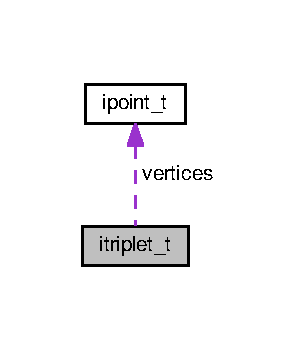
\includegraphics[width=143pt]{structitriplet__t__coll__graph}
\end{center}
\end{figure}
\subsection*{Data Fields}
\begin{DoxyCompactItemize}
\item 
struct \hyperlink{structipoint__t}{ipoint\-\_\-t} $\ast$ \hyperlink{structitriplet__t_a93f85fc4e829ca4d42b67173839af2c3}{vertices} \mbox{[}3\mbox{]}
\end{DoxyCompactItemize}


\subsection{Detailed Description}


Definition at line 24 of file iprimitives.\-h.



\subsection{Field Documentation}
\hypertarget{structitriplet__t_a93f85fc4e829ca4d42b67173839af2c3}{\index{itriplet\-\_\-t@{itriplet\-\_\-t}!vertices@{vertices}}
\index{vertices@{vertices}!itriplet_t@{itriplet\-\_\-t}}
\subsubsection[{vertices}]{\setlength{\rightskip}{0pt plus 5cm}struct {\bf ipoint\-\_\-t}$\ast$ itriplet\-\_\-t\-::vertices\mbox{[}3\mbox{]}}}\label{structitriplet__t_a93f85fc4e829ca4d42b67173839af2c3}


Definition at line 25 of file iprimitives.\-h.



The documentation for this struct was generated from the following file\-:\begin{DoxyCompactItemize}
\item 
src/\hyperlink{iprimitives_8h}{iprimitives.\-h}\end{DoxyCompactItemize}

\hypertarget{structivector__t}{\section{ivector\-\_\-t Struct Reference}
\label{structivector__t}\index{ivector\-\_\-t@{ivector\-\_\-t}}
}


{\ttfamily \#include $<$icoordinates.\-h$>$}

\subsection*{Data Fields}
\begin{DoxyCompactItemize}
\item 
double \hyperlink{structivector__t_a4b91a8fcb6a98d2ba8e2f5d483d7c577}{x}
\item 
double \hyperlink{structivector__t_af6af8ee13897aea97b1d8fe42bb83b17}{y}
\end{DoxyCompactItemize}


\subsection{Detailed Description}


Definition at line 52 of file icoordinates.\-h.



\subsection{Field Documentation}
\hypertarget{structivector__t_a4b91a8fcb6a98d2ba8e2f5d483d7c577}{\index{ivector\-\_\-t@{ivector\-\_\-t}!x@{x}}
\index{x@{x}!ivector_t@{ivector\-\_\-t}}
\subsubsection[{x}]{\setlength{\rightskip}{0pt plus 5cm}double ivector\-\_\-t\-::x}}\label{structivector__t_a4b91a8fcb6a98d2ba8e2f5d483d7c577}


Definition at line 53 of file icoordinates.\-h.

\hypertarget{structivector__t_af6af8ee13897aea97b1d8fe42bb83b17}{\index{ivector\-\_\-t@{ivector\-\_\-t}!y@{y}}
\index{y@{y}!ivector_t@{ivector\-\_\-t}}
\subsubsection[{y}]{\setlength{\rightskip}{0pt plus 5cm}double ivector\-\_\-t\-::y}}\label{structivector__t_af6af8ee13897aea97b1d8fe42bb83b17}


Definition at line 54 of file icoordinates.\-h.



The documentation for this struct was generated from the following file\-:\begin{DoxyCompactItemize}
\item 
src/\hyperlink{icoordinates_8h}{icoordinates.\-h}\end{DoxyCompactItemize}

\chapter{File Documentation}
\hypertarget{error_8c}{\section{src/error.c File Reference}
\label{error_8c}\index{src/error.\-c@{src/error.\-c}}
}
{\ttfamily \#include \char`\"{}error.\-h\char`\"{}}\\*
{\ttfamily \#include \char`\"{}iprettyconsole.\-h\char`\"{}}\\*
{\ttfamily \#include $<$stdlib.\-h$>$}\\*
{\ttfamily \#include $<$stdio.\-h$>$}\\*
Include dependency graph for error.\-c\-:\nopagebreak
\begin{figure}[H]
\begin{center}
\leavevmode
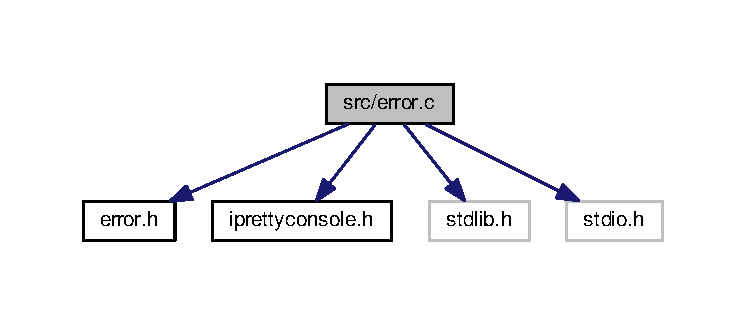
\includegraphics[width=350pt]{error_8c__incl}
\end{center}
\end{figure}
\subsection*{Functions}
\begin{DoxyCompactItemize}
\item 
int \hyperlink{error_8c_a3dccf4da7c4aabf6f10a72c80baa5b9f}{idie} (int error)
\item 
static void \hyperlink{error_8c_ac1727d6e8e99b92957a0a7099d19d6f4}{print\-\_\-error} (int error, char $\ast$message, int iswarning)
\item 
int \hyperlink{error_8c_ab10bea042bb9daa7a0e027197b8080e5}{ierror} (int error)
\end{DoxyCompactItemize}
\subsection*{Variables}
\begin{DoxyCompactItemize}
\item 
int \hyperlink{error_8c_a115185aff727ba2ac3079ebef145354d}{ishowerrors} = 1
\end{DoxyCompactItemize}


\subsection{Function Documentation}
\hypertarget{error_8c_a3dccf4da7c4aabf6f10a72c80baa5b9f}{\index{error.\-c@{error.\-c}!idie@{idie}}
\index{idie@{idie}!error.c@{error.\-c}}
\subsubsection[{idie}]{\setlength{\rightskip}{0pt plus 5cm}int idie (
\begin{DoxyParamCaption}
\item[{int}]{error}
\end{DoxyParamCaption}
)}}\label{error_8c_a3dccf4da7c4aabf6f10a72c80baa5b9f}
\hypertarget{error_8c_ab10bea042bb9daa7a0e027197b8080e5}{\index{error.\-c@{error.\-c}!ierror@{ierror}}
\index{ierror@{ierror}!error.c@{error.\-c}}
\subsubsection[{ierror}]{\setlength{\rightskip}{0pt plus 5cm}int ierror (
\begin{DoxyParamCaption}
\item[{int}]{error}
\end{DoxyParamCaption}
)}}\label{error_8c_ab10bea042bb9daa7a0e027197b8080e5}
Inferno's error handling function 
\begin{DoxyParams}{Parameters}
{\em error} & the error code that has been encountered \\
\hline
\end{DoxyParams}
\begin{DoxyReturn}{Returns}
an integer specifying the severity of the error 
\end{DoxyReturn}


Definition at line 29 of file error.\-c.


\begin{DoxyCode}
30 \{
31         \textcolor{keywordflow}{switch} (error) \{
32         \textcolor{keywordflow}{case} \hyperlink{error_8h_a06fc87d81c62e9abb8790b6e5713c55bac52ce3dc72e9de7cd173594b72138a02}{I\_INITIALIZATION\_ERROR}:
33                 \textcolor{keywordflow}{if}(\hyperlink{error_8c_a115185aff727ba2ac3079ebef145354d}{ishowerrors}) 
34                         \hyperlink{error_8c_ac1727d6e8e99b92957a0a7099d19d6f4}{print\_error}(\hyperlink{error_8h_a06fc87d81c62e9abb8790b6e5713c55bac52ce3dc72e9de7cd173594b72138a02}{I\_INITIALIZATION\_ERROR}, 
35                                     \textcolor{stringliteral}{"problem initializing inferno object."},
36                                     0
37                                    );
38                 \textcolor{keywordflow}{return} 1;
39         \textcolor{keywordflow}{case} \hyperlink{error_8h_a06fc87d81c62e9abb8790b6e5713c55ba4f043634eb144415a83e7e49adb15d4a}{I\_UNDEFINED\_EVENT\_HANDLER\_ERROR}:
40                 \textcolor{keywordflow}{if}(\hyperlink{error_8c_a115185aff727ba2ac3079ebef145354d}{ishowerrors}) 
41                         \hyperlink{error_8c_ac1727d6e8e99b92957a0a7099d19d6f4}{print\_error}(\hyperlink{error_8h_a06fc87d81c62e9abb8790b6e5713c55ba4f043634eb144415a83e7e49adb15d4a}{I\_UNDEFINED\_EVENT\_HANDLER\_ERROR}
      ,
42                                     \textcolor{stringliteral}{"trying to call an undefined event handler."},
43                                     1
44                                    );
45                 \textcolor{keywordflow}{return} 1;
46         \textcolor{keywordflow}{case} \hyperlink{error_8h_a06fc87d81c62e9abb8790b6e5713c55ba0155494d2502d24c87bdcab2830802de}{I\_NULL\_LINKED\_ERROR}:
47                 \textcolor{keywordflow}{if}(\hyperlink{error_8c_a115185aff727ba2ac3079ebef145354d}{ishowerrors}) 
48                         \hyperlink{error_8c_ac1727d6e8e99b92957a0a7099d19d6f4}{print\_error}(\hyperlink{error_8h_a06fc87d81c62e9abb8790b6e5713c55ba0155494d2502d24c87bdcab2830802de}{I\_NULL\_LINKED\_ERROR},
49                                     \textcolor{stringliteral}{"trying to access a null linked list element node."},
50                                     1
51                                    );
52                 \textcolor{keywordflow}{return} 2;
53         \textcolor{keywordflow}{case} \hyperlink{error_8h_a06fc87d81c62e9abb8790b6e5713c55ba67a045addd07db0dbf120c909105a375}{I\_BAD\_TRIPLET\_ERROR}:
54                 \textcolor{keywordflow}{if}(\hyperlink{error_8c_a115185aff727ba2ac3079ebef145354d}{ishowerrors}) 
55                         \hyperlink{error_8c_ac1727d6e8e99b92957a0a7099d19d6f4}{print\_error}(\hyperlink{error_8h_a06fc87d81c62e9abb8790b6e5713c55ba67a045addd07db0dbf120c909105a375}{I\_BAD\_TRIPLET\_ERROR},
56                                     \textcolor{stringliteral}{"trying to use a defective triplet, maybe two of the points
       accidentally have the same address or value?"},
57                                     0
58                                    );
59                 \textcolor{keywordflow}{return} 1;
60         \textcolor{keywordflow}{case} \hyperlink{error_8h_a06fc87d81c62e9abb8790b6e5713c55bad7fcde3f033c9c24f92c3afcb2bb3238}{I\_FRONTEND\_INITIALIZATION\_ERROR}:
61                 \textcolor{keywordflow}{if}(\hyperlink{error_8c_a115185aff727ba2ac3079ebef145354d}{ishowerrors}) 
62                         \hyperlink{error_8c_ac1727d6e8e99b92957a0a7099d19d6f4}{print\_error}(\hyperlink{error_8h_a06fc87d81c62e9abb8790b6e5713c55bad7fcde3f033c9c24f92c3afcb2bb3238}{I\_FRONTEND\_INITIALIZATION\_ERROR}
      ,
63                                     \textcolor{stringliteral}{"problem setting up your frontend."},
64                                     0
65                                    );
66                 \textcolor{keywordflow}{return} 2;
67         \textcolor{keywordflow}{case} \hyperlink{error_8h_a06fc87d81c62e9abb8790b6e5713c55ba1ed2580ed7646ff8fde5b8f10f476083}{I\_ERROR\_ERROR}:
68                 \textcolor{keywordflow}{if}(\hyperlink{error_8c_a115185aff727ba2ac3079ebef145354d}{ishowerrors}) 
69                         \hyperlink{error_8c_ac1727d6e8e99b92957a0a7099d19d6f4}{print\_error}(\hyperlink{error_8h_a06fc87d81c62e9abb8790b6e5713c55ba1ed2580ed7646ff8fde5b8f10f476083}{I\_ERROR\_ERROR},
70                                     \textcolor{stringliteral}{"trying to throw a nonexistent error."},
71                                     1
72                                    );
73                 \textcolor{keywordflow}{return} 1;
74         \textcolor{keywordflow}{case} \hyperlink{error_8h_a06fc87d81c62e9abb8790b6e5713c55ba5533863256dcb6d3efdfe981103a3120}{I\_IMPOSSIBLE\_ERROR}:
75                 \textcolor{keywordflow}{if} (\hyperlink{error_8c_a115185aff727ba2ac3079ebef145354d}{ishowerrors})
76                         \hyperlink{error_8c_ac1727d6e8e99b92957a0a7099d19d6f4}{print\_error}(\hyperlink{error_8h_a06fc87d81c62e9abb8790b6e5713c55ba5533863256dcb6d3efdfe981103a3120}{I\_IMPOSSIBLE\_ERROR},
77                                     \textcolor{stringliteral}{"the program has just reached a point that you thought was impossible
       to reach, and you decided to not handle it just in case, instead opting to make it throw the \(\backslash\)""} 
      \hyperlink{iprettyconsole_8h_a66290957baed5df3930ada4cb8caccf1}{KRED} \textcolor{stringliteral}{"I\_IMPOSSIBLE\_ERROR"} \hyperlink{iprettyconsole_8h_ab702106cf3b3e96750b6845ded4e0299}{RESET} \textcolor{stringliteral}{"\(\backslash\)" just to tempt fate."},
78                                     0);
79                 \textcolor{keywordflow}{return} 2;
80         \textcolor{keywordflow}{default}:
81                 \textcolor{keywordflow}{return} \hyperlink{error_8c_ab10bea042bb9daa7a0e027197b8080e5}{ierror}(\hyperlink{error_8h_a06fc87d81c62e9abb8790b6e5713c55ba1ed2580ed7646ff8fde5b8f10f476083}{I\_ERROR\_ERROR});
82         \}
83 \}
\end{DoxyCode}


Here is the call graph for this function\-:\nopagebreak
\begin{figure}[H]
\begin{center}
\leavevmode
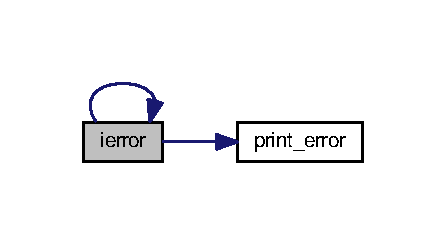
\includegraphics[width=214pt]{error_8c_ab10bea042bb9daa7a0e027197b8080e5_cgraph}
\end{center}
\end{figure}




Here is the caller graph for this function\-:
\nopagebreak
\begin{figure}[H]
\begin{center}
\leavevmode
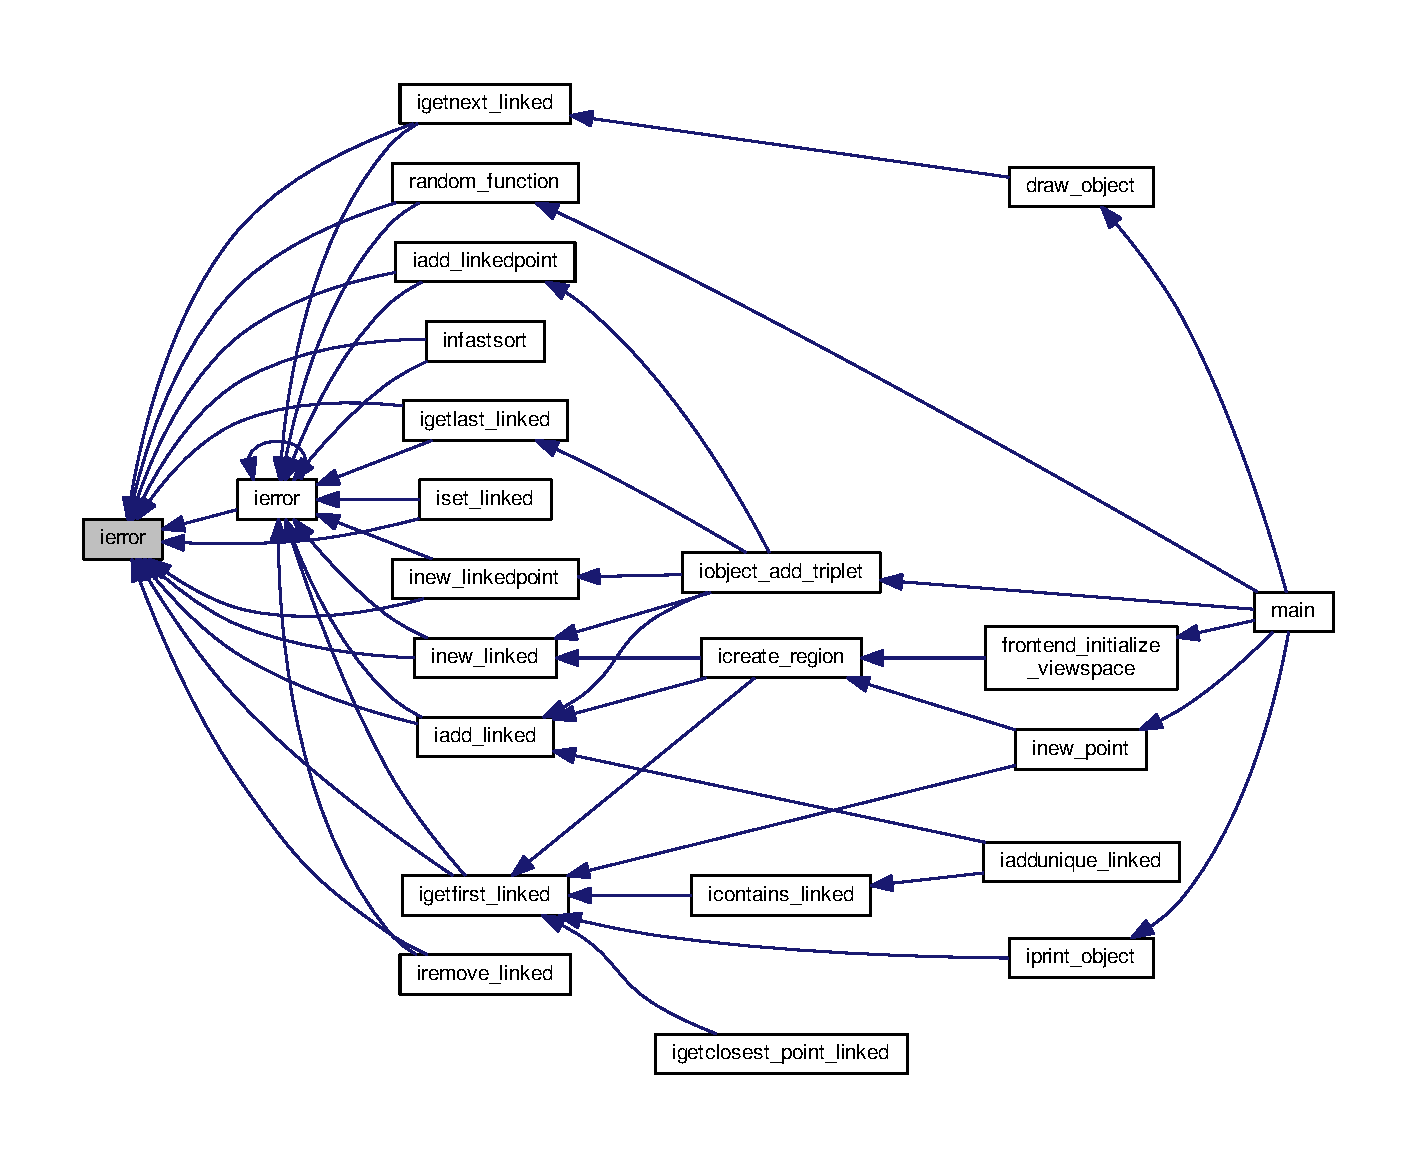
\includegraphics[width=350pt]{error_8c_ab10bea042bb9daa7a0e027197b8080e5_icgraph}
\end{center}
\end{figure}


\hypertarget{error_8c_ac1727d6e8e99b92957a0a7099d19d6f4}{\index{error.\-c@{error.\-c}!print\-\_\-error@{print\-\_\-error}}
\index{print\-\_\-error@{print\-\_\-error}!error.c@{error.\-c}}
\subsubsection[{print\-\_\-error}]{\setlength{\rightskip}{0pt plus 5cm}static void print\-\_\-error (
\begin{DoxyParamCaption}
\item[{int}]{error, }
\item[{char $\ast$}]{message, }
\item[{int}]{iswarning}
\end{DoxyParamCaption}
)\hspace{0.3cm}{\ttfamily [static]}}}\label{error_8c_ac1727d6e8e99b92957a0a7099d19d6f4}
Handles printing of errors. Static function, only to be called by ierror 
\begin{DoxyParams}{Parameters}
{\em error} & the integer code of the error to be printed \\
\hline
{\em $\ast$message} & the message to tell the user \\
\hline
{\em iswarning} & bool, determines the message prefix and its color \\
\hline
\end{DoxyParams}


Definition at line 15 of file error.\-c.


\begin{DoxyCode}
16 \{
17         \textcolor{keywordflow}{if} (iswarning)
18                 fprintf(stderr, \hyperlink{iprettyconsole_8h_a897b10d246533c95ba86cb79f92e465a}{KYEL} \textcolor{stringliteral}{"WARNING %d"} \hyperlink{iprettyconsole_8h_ab702106cf3b3e96750b6845ded4e0299}{RESET}, error);
19         \textcolor{keywordflow}{else}
20                 fprintf(stderr, \hyperlink{iprettyconsole_8h_a66290957baed5df3930ada4cb8caccf1}{KRED} \textcolor{stringliteral}{"ERROR %d"} \hyperlink{iprettyconsole_8h_ab702106cf3b3e96750b6845ded4e0299}{RESET}, error);
21         fprintf(stdout, \textcolor{stringliteral}{": %s\(\backslash\)n"}, message);
22         \textcolor{keywordflow}{return};
23 \}
\end{DoxyCode}


Here is the caller graph for this function\-:
\nopagebreak
\begin{figure}[H]
\begin{center}
\leavevmode
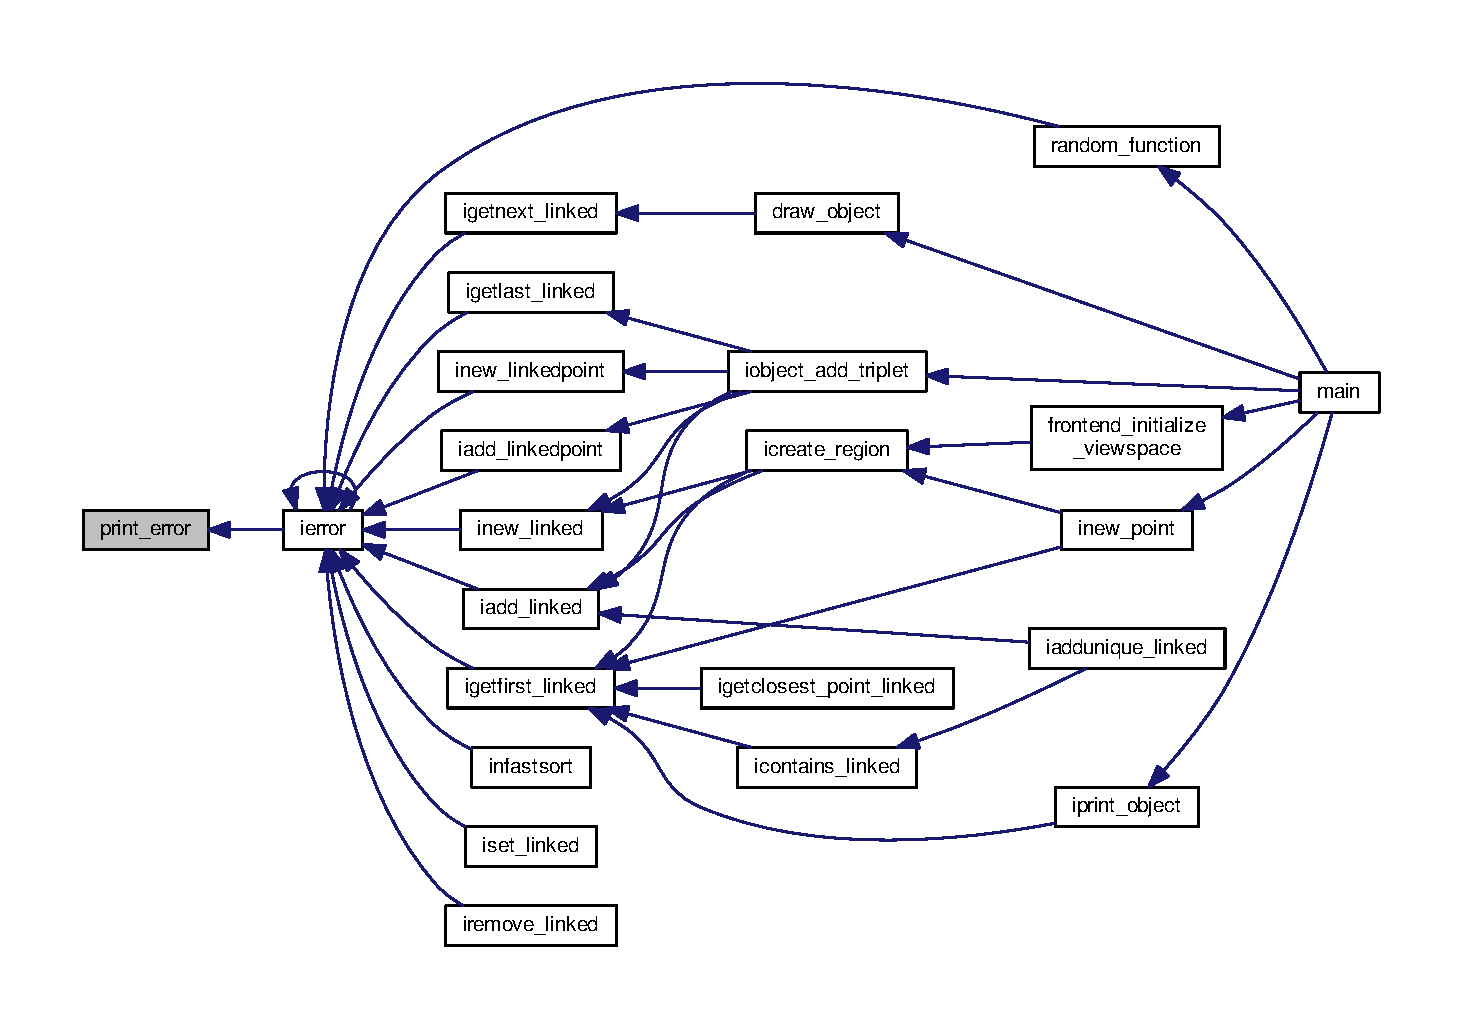
\includegraphics[width=350pt]{error_8c_ac1727d6e8e99b92957a0a7099d19d6f4_icgraph}
\end{center}
\end{figure}




\subsection{Variable Documentation}
\hypertarget{error_8c_a115185aff727ba2ac3079ebef145354d}{\index{error.\-c@{error.\-c}!ishowerrors@{ishowerrors}}
\index{ishowerrors@{ishowerrors}!error.c@{error.\-c}}
\subsubsection[{ishowerrors}]{\setlength{\rightskip}{0pt plus 5cm}int ishowerrors = 1}}\label{error_8c_a115185aff727ba2ac3079ebef145354d}


Definition at line 6 of file error.\-c.


\hypertarget{error_8h}{\section{src/error.h File Reference}
\label{error_8h}\index{src/error.\-h@{src/error.\-h}}
}
This graph shows which files directly or indirectly include this file\-:
\nopagebreak
\begin{figure}[H]
\begin{center}
\leavevmode
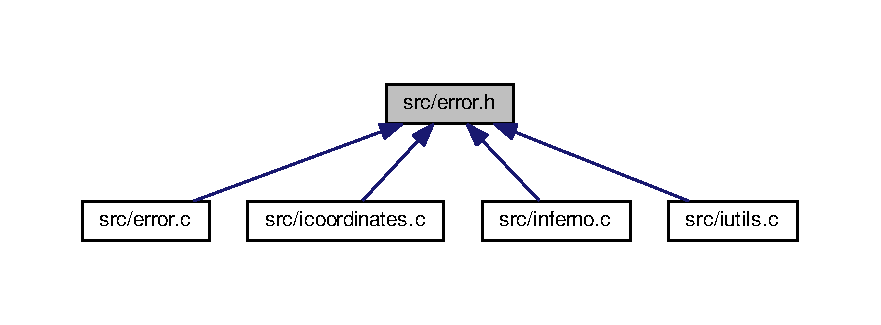
\includegraphics[width=350pt]{error_8h__dep__incl}
\end{center}
\end{figure}
\subsection*{Enumerations}
\begin{DoxyCompactItemize}
\item 
enum \{ \\*
\hyperlink{error_8h_a06fc87d81c62e9abb8790b6e5713c55bac52ce3dc72e9de7cd173594b72138a02}{I\-\_\-\-I\-N\-I\-T\-I\-A\-L\-I\-Z\-A\-T\-I\-O\-N\-\_\-\-E\-R\-R\-O\-R}, 
\hyperlink{error_8h_a06fc87d81c62e9abb8790b6e5713c55ba4f043634eb144415a83e7e49adb15d4a}{I\-\_\-\-U\-N\-D\-E\-F\-I\-N\-E\-D\-\_\-\-E\-V\-E\-N\-T\-\_\-\-H\-A\-N\-D\-L\-E\-R\-\_\-\-E\-R\-R\-O\-R}, 
\hyperlink{error_8h_a06fc87d81c62e9abb8790b6e5713c55ba0155494d2502d24c87bdcab2830802de}{I\-\_\-\-N\-U\-L\-L\-\_\-\-L\-I\-N\-K\-E\-D\-\_\-\-E\-R\-R\-O\-R}, 
\hyperlink{error_8h_a06fc87d81c62e9abb8790b6e5713c55ba67a045addd07db0dbf120c909105a375}{I\-\_\-\-B\-A\-D\-\_\-\-T\-R\-I\-P\-L\-E\-T\-\_\-\-E\-R\-R\-O\-R}, 
\\*
\hyperlink{error_8h_a06fc87d81c62e9abb8790b6e5713c55bad7fcde3f033c9c24f92c3afcb2bb3238}{I\-\_\-\-F\-R\-O\-N\-T\-E\-N\-D\-\_\-\-I\-N\-I\-T\-I\-A\-L\-I\-Z\-A\-T\-I\-O\-N\-\_\-\-E\-R\-R\-O\-R}, 
\hyperlink{error_8h_a06fc87d81c62e9abb8790b6e5713c55ba1ed2580ed7646ff8fde5b8f10f476083}{I\-\_\-\-E\-R\-R\-O\-R\-\_\-\-E\-R\-R\-O\-R}, 
\hyperlink{error_8h_a06fc87d81c62e9abb8790b6e5713c55ba5533863256dcb6d3efdfe981103a3120}{I\-\_\-\-I\-M\-P\-O\-S\-S\-I\-B\-L\-E\-\_\-\-E\-R\-R\-O\-R}
 \}
\end{DoxyCompactItemize}
\subsection*{Functions}
\begin{DoxyCompactItemize}
\item 
int \hyperlink{error_8h_a3dccf4da7c4aabf6f10a72c80baa5b9f}{idie} (int error)
\item 
int \hyperlink{error_8h_ab10bea042bb9daa7a0e027197b8080e5}{ierror} (int error)
\end{DoxyCompactItemize}
\subsection*{Variables}
\begin{DoxyCompactItemize}
\item 
enum  \{ ... \}  \hyperlink{error_8h_a073732e2eb29171be27f9d205b78ea59}{inferno\-\_\-errors}
\item 
int \hyperlink{error_8h_a115185aff727ba2ac3079ebef145354d}{ishowerrors}
\end{DoxyCompactItemize}


\subsection{Enumeration Type Documentation}
\hypertarget{error_8h_a06fc87d81c62e9abb8790b6e5713c55b}{\subsubsection[{anonymous enum}]{\setlength{\rightskip}{0pt plus 5cm}anonymous enum}}\label{error_8h_a06fc87d81c62e9abb8790b6e5713c55b}
\begin{Desc}
\item[Enumerator]\par
\begin{description}
\index{I\-\_\-\-I\-N\-I\-T\-I\-A\-L\-I\-Z\-A\-T\-I\-O\-N\-\_\-\-E\-R\-R\-O\-R@{I\-\_\-\-I\-N\-I\-T\-I\-A\-L\-I\-Z\-A\-T\-I\-O\-N\-\_\-\-E\-R\-R\-O\-R}!error.\-h@{error.\-h}}\index{error.\-h@{error.\-h}!I\-\_\-\-I\-N\-I\-T\-I\-A\-L\-I\-Z\-A\-T\-I\-O\-N\-\_\-\-E\-R\-R\-O\-R@{I\-\_\-\-I\-N\-I\-T\-I\-A\-L\-I\-Z\-A\-T\-I\-O\-N\-\_\-\-E\-R\-R\-O\-R}}\item[{\em 
\hypertarget{error_8h_a06fc87d81c62e9abb8790b6e5713c55bac52ce3dc72e9de7cd173594b72138a02}{I\-\_\-\-I\-N\-I\-T\-I\-A\-L\-I\-Z\-A\-T\-I\-O\-N\-\_\-\-E\-R\-R\-O\-R}\label{error_8h_a06fc87d81c62e9abb8790b6e5713c55bac52ce3dc72e9de7cd173594b72138a02}
}]\index{I\-\_\-\-U\-N\-D\-E\-F\-I\-N\-E\-D\-\_\-\-E\-V\-E\-N\-T\-\_\-\-H\-A\-N\-D\-L\-E\-R\-\_\-\-E\-R\-R\-O\-R@{I\-\_\-\-U\-N\-D\-E\-F\-I\-N\-E\-D\-\_\-\-E\-V\-E\-N\-T\-\_\-\-H\-A\-N\-D\-L\-E\-R\-\_\-\-E\-R\-R\-O\-R}!error.\-h@{error.\-h}}\index{error.\-h@{error.\-h}!I\-\_\-\-U\-N\-D\-E\-F\-I\-N\-E\-D\-\_\-\-E\-V\-E\-N\-T\-\_\-\-H\-A\-N\-D\-L\-E\-R\-\_\-\-E\-R\-R\-O\-R@{I\-\_\-\-U\-N\-D\-E\-F\-I\-N\-E\-D\-\_\-\-E\-V\-E\-N\-T\-\_\-\-H\-A\-N\-D\-L\-E\-R\-\_\-\-E\-R\-R\-O\-R}}\item[{\em 
\hypertarget{error_8h_a06fc87d81c62e9abb8790b6e5713c55ba4f043634eb144415a83e7e49adb15d4a}{I\-\_\-\-U\-N\-D\-E\-F\-I\-N\-E\-D\-\_\-\-E\-V\-E\-N\-T\-\_\-\-H\-A\-N\-D\-L\-E\-R\-\_\-\-E\-R\-R\-O\-R}\label{error_8h_a06fc87d81c62e9abb8790b6e5713c55ba4f043634eb144415a83e7e49adb15d4a}
}]\index{I\-\_\-\-N\-U\-L\-L\-\_\-\-L\-I\-N\-K\-E\-D\-\_\-\-E\-R\-R\-O\-R@{I\-\_\-\-N\-U\-L\-L\-\_\-\-L\-I\-N\-K\-E\-D\-\_\-\-E\-R\-R\-O\-R}!error.\-h@{error.\-h}}\index{error.\-h@{error.\-h}!I\-\_\-\-N\-U\-L\-L\-\_\-\-L\-I\-N\-K\-E\-D\-\_\-\-E\-R\-R\-O\-R@{I\-\_\-\-N\-U\-L\-L\-\_\-\-L\-I\-N\-K\-E\-D\-\_\-\-E\-R\-R\-O\-R}}\item[{\em 
\hypertarget{error_8h_a06fc87d81c62e9abb8790b6e5713c55ba0155494d2502d24c87bdcab2830802de}{I\-\_\-\-N\-U\-L\-L\-\_\-\-L\-I\-N\-K\-E\-D\-\_\-\-E\-R\-R\-O\-R}\label{error_8h_a06fc87d81c62e9abb8790b6e5713c55ba0155494d2502d24c87bdcab2830802de}
}]\index{I\-\_\-\-B\-A\-D\-\_\-\-T\-R\-I\-P\-L\-E\-T\-\_\-\-E\-R\-R\-O\-R@{I\-\_\-\-B\-A\-D\-\_\-\-T\-R\-I\-P\-L\-E\-T\-\_\-\-E\-R\-R\-O\-R}!error.\-h@{error.\-h}}\index{error.\-h@{error.\-h}!I\-\_\-\-B\-A\-D\-\_\-\-T\-R\-I\-P\-L\-E\-T\-\_\-\-E\-R\-R\-O\-R@{I\-\_\-\-B\-A\-D\-\_\-\-T\-R\-I\-P\-L\-E\-T\-\_\-\-E\-R\-R\-O\-R}}\item[{\em 
\hypertarget{error_8h_a06fc87d81c62e9abb8790b6e5713c55ba67a045addd07db0dbf120c909105a375}{I\-\_\-\-B\-A\-D\-\_\-\-T\-R\-I\-P\-L\-E\-T\-\_\-\-E\-R\-R\-O\-R}\label{error_8h_a06fc87d81c62e9abb8790b6e5713c55ba67a045addd07db0dbf120c909105a375}
}]\index{I\-\_\-\-F\-R\-O\-N\-T\-E\-N\-D\-\_\-\-I\-N\-I\-T\-I\-A\-L\-I\-Z\-A\-T\-I\-O\-N\-\_\-\-E\-R\-R\-O\-R@{I\-\_\-\-F\-R\-O\-N\-T\-E\-N\-D\-\_\-\-I\-N\-I\-T\-I\-A\-L\-I\-Z\-A\-T\-I\-O\-N\-\_\-\-E\-R\-R\-O\-R}!error.\-h@{error.\-h}}\index{error.\-h@{error.\-h}!I\-\_\-\-F\-R\-O\-N\-T\-E\-N\-D\-\_\-\-I\-N\-I\-T\-I\-A\-L\-I\-Z\-A\-T\-I\-O\-N\-\_\-\-E\-R\-R\-O\-R@{I\-\_\-\-F\-R\-O\-N\-T\-E\-N\-D\-\_\-\-I\-N\-I\-T\-I\-A\-L\-I\-Z\-A\-T\-I\-O\-N\-\_\-\-E\-R\-R\-O\-R}}\item[{\em 
\hypertarget{error_8h_a06fc87d81c62e9abb8790b6e5713c55bad7fcde3f033c9c24f92c3afcb2bb3238}{I\-\_\-\-F\-R\-O\-N\-T\-E\-N\-D\-\_\-\-I\-N\-I\-T\-I\-A\-L\-I\-Z\-A\-T\-I\-O\-N\-\_\-\-E\-R\-R\-O\-R}\label{error_8h_a06fc87d81c62e9abb8790b6e5713c55bad7fcde3f033c9c24f92c3afcb2bb3238}
}]\index{I\-\_\-\-E\-R\-R\-O\-R\-\_\-\-E\-R\-R\-O\-R@{I\-\_\-\-E\-R\-R\-O\-R\-\_\-\-E\-R\-R\-O\-R}!error.\-h@{error.\-h}}\index{error.\-h@{error.\-h}!I\-\_\-\-E\-R\-R\-O\-R\-\_\-\-E\-R\-R\-O\-R@{I\-\_\-\-E\-R\-R\-O\-R\-\_\-\-E\-R\-R\-O\-R}}\item[{\em 
\hypertarget{error_8h_a06fc87d81c62e9abb8790b6e5713c55ba1ed2580ed7646ff8fde5b8f10f476083}{I\-\_\-\-E\-R\-R\-O\-R\-\_\-\-E\-R\-R\-O\-R}\label{error_8h_a06fc87d81c62e9abb8790b6e5713c55ba1ed2580ed7646ff8fde5b8f10f476083}
}]\index{I\-\_\-\-I\-M\-P\-O\-S\-S\-I\-B\-L\-E\-\_\-\-E\-R\-R\-O\-R@{I\-\_\-\-I\-M\-P\-O\-S\-S\-I\-B\-L\-E\-\_\-\-E\-R\-R\-O\-R}!error.\-h@{error.\-h}}\index{error.\-h@{error.\-h}!I\-\_\-\-I\-M\-P\-O\-S\-S\-I\-B\-L\-E\-\_\-\-E\-R\-R\-O\-R@{I\-\_\-\-I\-M\-P\-O\-S\-S\-I\-B\-L\-E\-\_\-\-E\-R\-R\-O\-R}}\item[{\em 
\hypertarget{error_8h_a06fc87d81c62e9abb8790b6e5713c55ba5533863256dcb6d3efdfe981103a3120}{I\-\_\-\-I\-M\-P\-O\-S\-S\-I\-B\-L\-E\-\_\-\-E\-R\-R\-O\-R}\label{error_8h_a06fc87d81c62e9abb8790b6e5713c55ba5533863256dcb6d3efdfe981103a3120}
}]\end{description}
\end{Desc}


Definition at line 4 of file error.\-h.


\begin{DoxyCode}
4      \{
5         \hyperlink{error_8h_a06fc87d81c62e9abb8790b6e5713c55bac52ce3dc72e9de7cd173594b72138a02}{I\_INITIALIZATION\_ERROR},
6         \hyperlink{error_8h_a06fc87d81c62e9abb8790b6e5713c55ba4f043634eb144415a83e7e49adb15d4a}{I\_UNDEFINED\_EVENT\_HANDLER\_ERROR},
7         \hyperlink{error_8h_a06fc87d81c62e9abb8790b6e5713c55ba0155494d2502d24c87bdcab2830802de}{I\_NULL\_LINKED\_ERROR},
8         \hyperlink{error_8h_a06fc87d81c62e9abb8790b6e5713c55ba67a045addd07db0dbf120c909105a375}{I\_BAD\_TRIPLET\_ERROR},
9         \hyperlink{error_8h_a06fc87d81c62e9abb8790b6e5713c55bad7fcde3f033c9c24f92c3afcb2bb3238}{I\_FRONTEND\_INITIALIZATION\_ERROR},
10         \hyperlink{error_8h_a06fc87d81c62e9abb8790b6e5713c55ba1ed2580ed7646ff8fde5b8f10f476083}{I\_ERROR\_ERROR},
11         \hyperlink{error_8h_a06fc87d81c62e9abb8790b6e5713c55ba5533863256dcb6d3efdfe981103a3120}{I\_IMPOSSIBLE\_ERROR}
12 \} \hyperlink{error_8h_a073732e2eb29171be27f9d205b78ea59}{inferno\_errors};
\end{DoxyCode}


\subsection{Function Documentation}
\hypertarget{error_8h_a3dccf4da7c4aabf6f10a72c80baa5b9f}{\index{error.\-h@{error.\-h}!idie@{idie}}
\index{idie@{idie}!error.h@{error.\-h}}
\subsubsection[{idie}]{\setlength{\rightskip}{0pt plus 5cm}int idie (
\begin{DoxyParamCaption}
\item[{int}]{error}
\end{DoxyParamCaption}
)}}\label{error_8h_a3dccf4da7c4aabf6f10a72c80baa5b9f}
\hypertarget{error_8h_ab10bea042bb9daa7a0e027197b8080e5}{\index{error.\-h@{error.\-h}!ierror@{ierror}}
\index{ierror@{ierror}!error.h@{error.\-h}}
\subsubsection[{ierror}]{\setlength{\rightskip}{0pt plus 5cm}int ierror (
\begin{DoxyParamCaption}
\item[{int}]{error}
\end{DoxyParamCaption}
)}}\label{error_8h_ab10bea042bb9daa7a0e027197b8080e5}
Inferno's error handling function 
\begin{DoxyParams}{Parameters}
{\em error} & the error code that has been encountered \\
\hline
\end{DoxyParams}
\begin{DoxyReturn}{Returns}
an integer specifying the severity of the error 
\end{DoxyReturn}


Definition at line 29 of file error.\-c.


\begin{DoxyCode}
30 \{
31         \textcolor{keywordflow}{switch} (error) \{
32         \textcolor{keywordflow}{case} \hyperlink{error_8h_a06fc87d81c62e9abb8790b6e5713c55bac52ce3dc72e9de7cd173594b72138a02}{I\_INITIALIZATION\_ERROR}:
33                 \textcolor{keywordflow}{if}(\hyperlink{error_8c_a115185aff727ba2ac3079ebef145354d}{ishowerrors}) 
34                         \hyperlink{error_8c_ac1727d6e8e99b92957a0a7099d19d6f4}{print\_error}(\hyperlink{error_8h_a06fc87d81c62e9abb8790b6e5713c55bac52ce3dc72e9de7cd173594b72138a02}{I\_INITIALIZATION\_ERROR}, 
35                                     \textcolor{stringliteral}{"problem initializing inferno object."},
36                                     0
37                                    );
38                 \textcolor{keywordflow}{return} 1;
39         \textcolor{keywordflow}{case} \hyperlink{error_8h_a06fc87d81c62e9abb8790b6e5713c55ba4f043634eb144415a83e7e49adb15d4a}{I\_UNDEFINED\_EVENT\_HANDLER\_ERROR}:
40                 \textcolor{keywordflow}{if}(\hyperlink{error_8c_a115185aff727ba2ac3079ebef145354d}{ishowerrors}) 
41                         \hyperlink{error_8c_ac1727d6e8e99b92957a0a7099d19d6f4}{print\_error}(\hyperlink{error_8h_a06fc87d81c62e9abb8790b6e5713c55ba4f043634eb144415a83e7e49adb15d4a}{I\_UNDEFINED\_EVENT\_HANDLER\_ERROR}
      ,
42                                     \textcolor{stringliteral}{"trying to call an undefined event handler."},
43                                     1
44                                    );
45                 \textcolor{keywordflow}{return} 1;
46         \textcolor{keywordflow}{case} \hyperlink{error_8h_a06fc87d81c62e9abb8790b6e5713c55ba0155494d2502d24c87bdcab2830802de}{I\_NULL\_LINKED\_ERROR}:
47                 \textcolor{keywordflow}{if}(\hyperlink{error_8c_a115185aff727ba2ac3079ebef145354d}{ishowerrors}) 
48                         \hyperlink{error_8c_ac1727d6e8e99b92957a0a7099d19d6f4}{print\_error}(\hyperlink{error_8h_a06fc87d81c62e9abb8790b6e5713c55ba0155494d2502d24c87bdcab2830802de}{I\_NULL\_LINKED\_ERROR},
49                                     \textcolor{stringliteral}{"trying to access a null linked list element node."},
50                                     1
51                                    );
52                 \textcolor{keywordflow}{return} 2;
53         \textcolor{keywordflow}{case} \hyperlink{error_8h_a06fc87d81c62e9abb8790b6e5713c55ba67a045addd07db0dbf120c909105a375}{I\_BAD\_TRIPLET\_ERROR}:
54                 \textcolor{keywordflow}{if}(\hyperlink{error_8c_a115185aff727ba2ac3079ebef145354d}{ishowerrors}) 
55                         \hyperlink{error_8c_ac1727d6e8e99b92957a0a7099d19d6f4}{print\_error}(\hyperlink{error_8h_a06fc87d81c62e9abb8790b6e5713c55ba67a045addd07db0dbf120c909105a375}{I\_BAD\_TRIPLET\_ERROR},
56                                     \textcolor{stringliteral}{"trying to use a defective triplet, maybe two of the points
       accidentally have the same address or value?"},
57                                     0
58                                    );
59                 \textcolor{keywordflow}{return} 1;
60         \textcolor{keywordflow}{case} \hyperlink{error_8h_a06fc87d81c62e9abb8790b6e5713c55bad7fcde3f033c9c24f92c3afcb2bb3238}{I\_FRONTEND\_INITIALIZATION\_ERROR}:
61                 \textcolor{keywordflow}{if}(\hyperlink{error_8c_a115185aff727ba2ac3079ebef145354d}{ishowerrors}) 
62                         \hyperlink{error_8c_ac1727d6e8e99b92957a0a7099d19d6f4}{print\_error}(\hyperlink{error_8h_a06fc87d81c62e9abb8790b6e5713c55bad7fcde3f033c9c24f92c3afcb2bb3238}{I\_FRONTEND\_INITIALIZATION\_ERROR}
      ,
63                                     \textcolor{stringliteral}{"problem setting up your frontend."},
64                                     0
65                                    );
66                 \textcolor{keywordflow}{return} 2;
67         \textcolor{keywordflow}{case} \hyperlink{error_8h_a06fc87d81c62e9abb8790b6e5713c55ba1ed2580ed7646ff8fde5b8f10f476083}{I\_ERROR\_ERROR}:
68                 \textcolor{keywordflow}{if}(\hyperlink{error_8c_a115185aff727ba2ac3079ebef145354d}{ishowerrors}) 
69                         \hyperlink{error_8c_ac1727d6e8e99b92957a0a7099d19d6f4}{print\_error}(\hyperlink{error_8h_a06fc87d81c62e9abb8790b6e5713c55ba1ed2580ed7646ff8fde5b8f10f476083}{I\_ERROR\_ERROR},
70                                     \textcolor{stringliteral}{"trying to throw a nonexistent error."},
71                                     1
72                                    );
73                 \textcolor{keywordflow}{return} 1;
74         \textcolor{keywordflow}{case} \hyperlink{error_8h_a06fc87d81c62e9abb8790b6e5713c55ba5533863256dcb6d3efdfe981103a3120}{I\_IMPOSSIBLE\_ERROR}:
75                 \textcolor{keywordflow}{if} (\hyperlink{error_8c_a115185aff727ba2ac3079ebef145354d}{ishowerrors})
76                         \hyperlink{error_8c_ac1727d6e8e99b92957a0a7099d19d6f4}{print\_error}(\hyperlink{error_8h_a06fc87d81c62e9abb8790b6e5713c55ba5533863256dcb6d3efdfe981103a3120}{I\_IMPOSSIBLE\_ERROR},
77                                     \textcolor{stringliteral}{"the program has just reached a point that you thought was impossible
       to reach, and you decided to not handle it just in case, instead opting to make it throw the \(\backslash\)""} 
      \hyperlink{iprettyconsole_8h_a66290957baed5df3930ada4cb8caccf1}{KRED} \textcolor{stringliteral}{"I\_IMPOSSIBLE\_ERROR"} \hyperlink{iprettyconsole_8h_ab702106cf3b3e96750b6845ded4e0299}{RESET} \textcolor{stringliteral}{"\(\backslash\)" just to tempt fate."},
78                                     0);
79                 \textcolor{keywordflow}{return} 2;
80         \textcolor{keywordflow}{default}:
81                 \textcolor{keywordflow}{return} \hyperlink{error_8c_ab10bea042bb9daa7a0e027197b8080e5}{ierror}(\hyperlink{error_8h_a06fc87d81c62e9abb8790b6e5713c55ba1ed2580ed7646ff8fde5b8f10f476083}{I\_ERROR\_ERROR});
82         \}
83 \}
\end{DoxyCode}


Here is the call graph for this function\-:\nopagebreak
\begin{figure}[H]
\begin{center}
\leavevmode
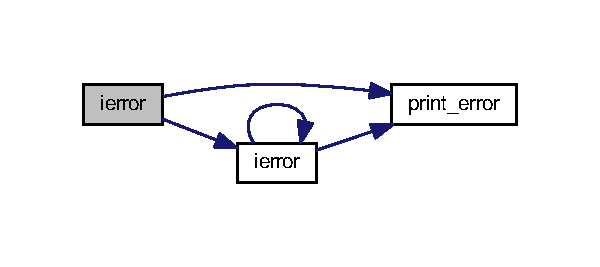
\includegraphics[width=288pt]{error_8h_ab10bea042bb9daa7a0e027197b8080e5_cgraph}
\end{center}
\end{figure}




Here is the caller graph for this function\-:
\nopagebreak
\begin{figure}[H]
\begin{center}
\leavevmode
\includegraphics[width=350pt]{error_8h_ab10bea042bb9daa7a0e027197b8080e5_icgraph}
\end{center}
\end{figure}




\subsection{Variable Documentation}
\hypertarget{error_8h_a073732e2eb29171be27f9d205b78ea59}{\index{error.\-h@{error.\-h}!inferno\-\_\-errors@{inferno\-\_\-errors}}
\index{inferno\-\_\-errors@{inferno\-\_\-errors}!error.h@{error.\-h}}
\subsubsection[{inferno\-\_\-errors}]{\setlength{\rightskip}{0pt plus 5cm}enum \{ ... \}   inferno\-\_\-errors}}\label{error_8h_a073732e2eb29171be27f9d205b78ea59}
\hypertarget{error_8h_a115185aff727ba2ac3079ebef145354d}{\index{error.\-h@{error.\-h}!ishowerrors@{ishowerrors}}
\index{ishowerrors@{ishowerrors}!error.h@{error.\-h}}
\subsubsection[{ishowerrors}]{\setlength{\rightskip}{0pt plus 5cm}int ishowerrors}}\label{error_8h_a115185aff727ba2ac3079ebef145354d}


Definition at line 14 of file error.\-h.


\hypertarget{frontend_8c}{\section{src/frontends/frontend.c File Reference}
\label{frontend_8c}\index{src/frontends/frontend.\-c@{src/frontends/frontend.\-c}}
}
{\ttfamily \#include $<$stdlib.\-h$>$}\\*
{\ttfamily \#include \char`\"{}frontend.\-h\char`\"{}}\\*
Include dependency graph for frontend.\-c\-:\nopagebreak
\begin{figure}[H]
\begin{center}
\leavevmode
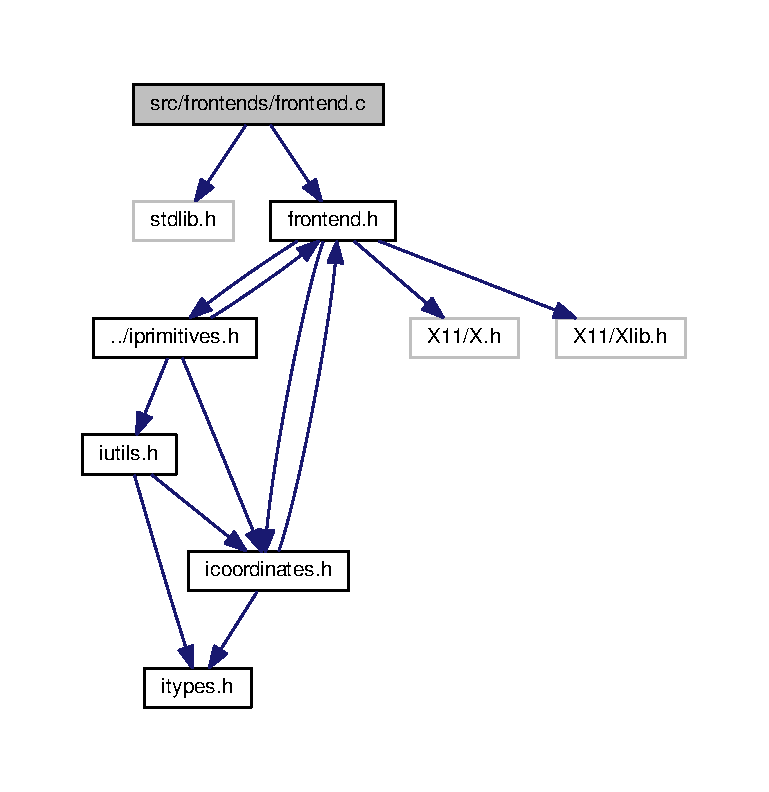
\includegraphics[width=350pt]{frontend_8c__incl}
\end{center}
\end{figure}
\subsection*{Functions}
\begin{DoxyCompactItemize}
\item 
struct \hyperlink{structievent__handler}{ievent\-\_\-handler} $\ast$ \hyperlink{frontend_8c_af20744b431ee1afa0043f15e5e2f9207}{inew\-\_\-eventhandler} (void $\ast$($\ast$handler)(void $\ast$args, void $\ast$event), void $\ast$args, unsigned short key\-\_\-code)
\item 
void \hyperlink{frontend_8c_a3012f53c007b67ba7dedf3156eb37e80}{frontend\-\_\-set\-\_\-eventhandler} (unsigned short i, char down, struct \hyperlink{structievent__handler}{ievent\-\_\-handler} $\ast$h, struct \hyperlink{structifrontendstate__t}{ifrontendstate\-\_\-t} $\ast$state)
\end{DoxyCompactItemize}


\subsection{Function Documentation}
\hypertarget{frontend_8c_a3012f53c007b67ba7dedf3156eb37e80}{\index{frontend.\-c@{frontend.\-c}!frontend\-\_\-set\-\_\-eventhandler@{frontend\-\_\-set\-\_\-eventhandler}}
\index{frontend\-\_\-set\-\_\-eventhandler@{frontend\-\_\-set\-\_\-eventhandler}!frontend.c@{frontend.\-c}}
\subsubsection[{frontend\-\_\-set\-\_\-eventhandler}]{\setlength{\rightskip}{0pt plus 5cm}void frontend\-\_\-set\-\_\-eventhandler (
\begin{DoxyParamCaption}
\item[{unsigned short}]{i, }
\item[{char}]{down, }
\item[{struct {\bf ievent\-\_\-handler} $\ast$}]{h, }
\item[{struct {\bf ifrontendstate\-\_\-t} $\ast$}]{state}
\end{DoxyParamCaption}
)}}\label{frontend_8c_a3012f53c007b67ba7dedf3156eb37e80}


Definition at line 31 of file frontend.\-c.


\begin{DoxyCode}
32 \{
33         \textcolor{keywordflow}{if} (down)
34                 state->\hyperlink{structifrontendstate__t_ad8fd468eaec37b949af562b39ad20d5a}{onkeydown\_handlers}[i] = h;
35         \textcolor{keywordflow}{else}
36                 state->\hyperlink{structifrontendstate__t_a5bb9423c4ba5f86cd8a0d50575031952}{onkeyup\_handlers}[i] = h;
37 \}
\end{DoxyCode}


Here is the caller graph for this function\-:\nopagebreak
\begin{figure}[H]
\begin{center}
\leavevmode
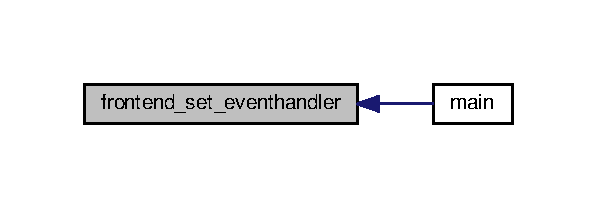
\includegraphics[width=286pt]{frontend_8c_a3012f53c007b67ba7dedf3156eb37e80_icgraph}
\end{center}
\end{figure}


\hypertarget{frontend_8c_af20744b431ee1afa0043f15e5e2f9207}{\index{frontend.\-c@{frontend.\-c}!inew\-\_\-eventhandler@{inew\-\_\-eventhandler}}
\index{inew\-\_\-eventhandler@{inew\-\_\-eventhandler}!frontend.c@{frontend.\-c}}
\subsubsection[{inew\-\_\-eventhandler}]{\setlength{\rightskip}{0pt plus 5cm}struct {\bf ievent\-\_\-handler}$\ast$ inew\-\_\-eventhandler (
\begin{DoxyParamCaption}
\item[{void $\ast$($\ast$)(void $\ast$args, void $\ast$event)}]{handler, }
\item[{void $\ast$}]{args, }
\item[{unsigned short}]{key\-\_\-code}
\end{DoxyParamCaption}
)}}\label{frontend_8c_af20744b431ee1afa0043f15e5e2f9207}


Definition at line 22 of file frontend.\-c.


\begin{DoxyCode}
23 \{
24         \textcolor{keyword}{struct }\hyperlink{structievent__handler}{ievent\_handler} *rval = malloc(\textcolor{keyword}{sizeof}(\textcolor{keyword}{struct} 
      \hyperlink{structievent__handler}{ievent\_handler}));
25         rval->\hyperlink{structievent__handler_a320eaffc01d119279ead9c5ad877c6da}{handler} = \hyperlink{structievent__handler_a320eaffc01d119279ead9c5ad877c6da}{handler};
26         rval->\hyperlink{structievent__handler_ac6b4e6b5b95ada7b0d9985f738ffe1e5}{args} = \hyperlink{structievent__handler_ac6b4e6b5b95ada7b0d9985f738ffe1e5}{args};
27         rval->\hyperlink{structievent__handler_af2766b148965989b8d202b11b9e72f60}{key\_code} = \hyperlink{structievent__handler_af2766b148965989b8d202b11b9e72f60}{key\_code};
28         \textcolor{keywordflow}{return} rval;
29 \}
\end{DoxyCode}


Here is the caller graph for this function\-:\nopagebreak
\begin{figure}[H]
\begin{center}
\leavevmode
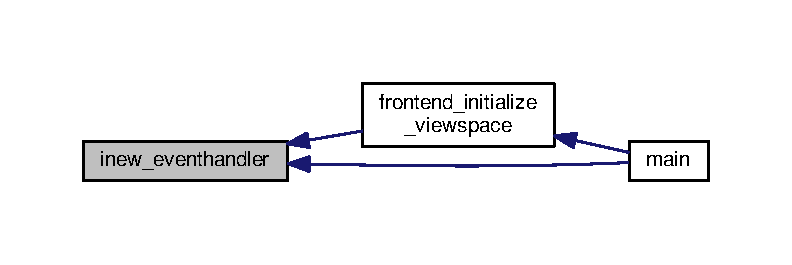
\includegraphics[width=350pt]{frontend_8c_af20744b431ee1afa0043f15e5e2f9207_icgraph}
\end{center}
\end{figure}



\hypertarget{frontend_8h}{\section{src/frontends/frontend.h File Reference}
\label{frontend_8h}\index{src/frontends/frontend.\-h@{src/frontends/frontend.\-h}}
}
{\ttfamily \#include \char`\"{}../iprimitives.\-h\char`\"{}}\\*
{\ttfamily \#include \char`\"{}../icoordinates.\-h\char`\"{}}\\*
{\ttfamily \#include $<$X11/\-X.\-h$>$}\\*
{\ttfamily \#include $<$X11/\-Xlib.\-h$>$}\\*
Include dependency graph for frontend.\-h\-:\nopagebreak
\begin{figure}[H]
\begin{center}
\leavevmode
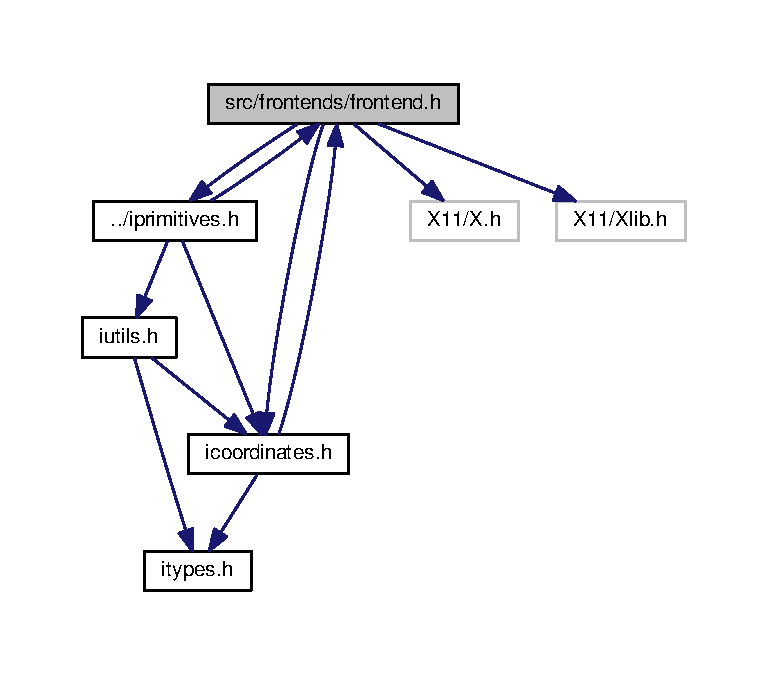
\includegraphics[width=350pt]{frontend_8h__incl}
\end{center}
\end{figure}
This graph shows which files directly or indirectly include this file\-:
\nopagebreak
\begin{figure}[H]
\begin{center}
\leavevmode
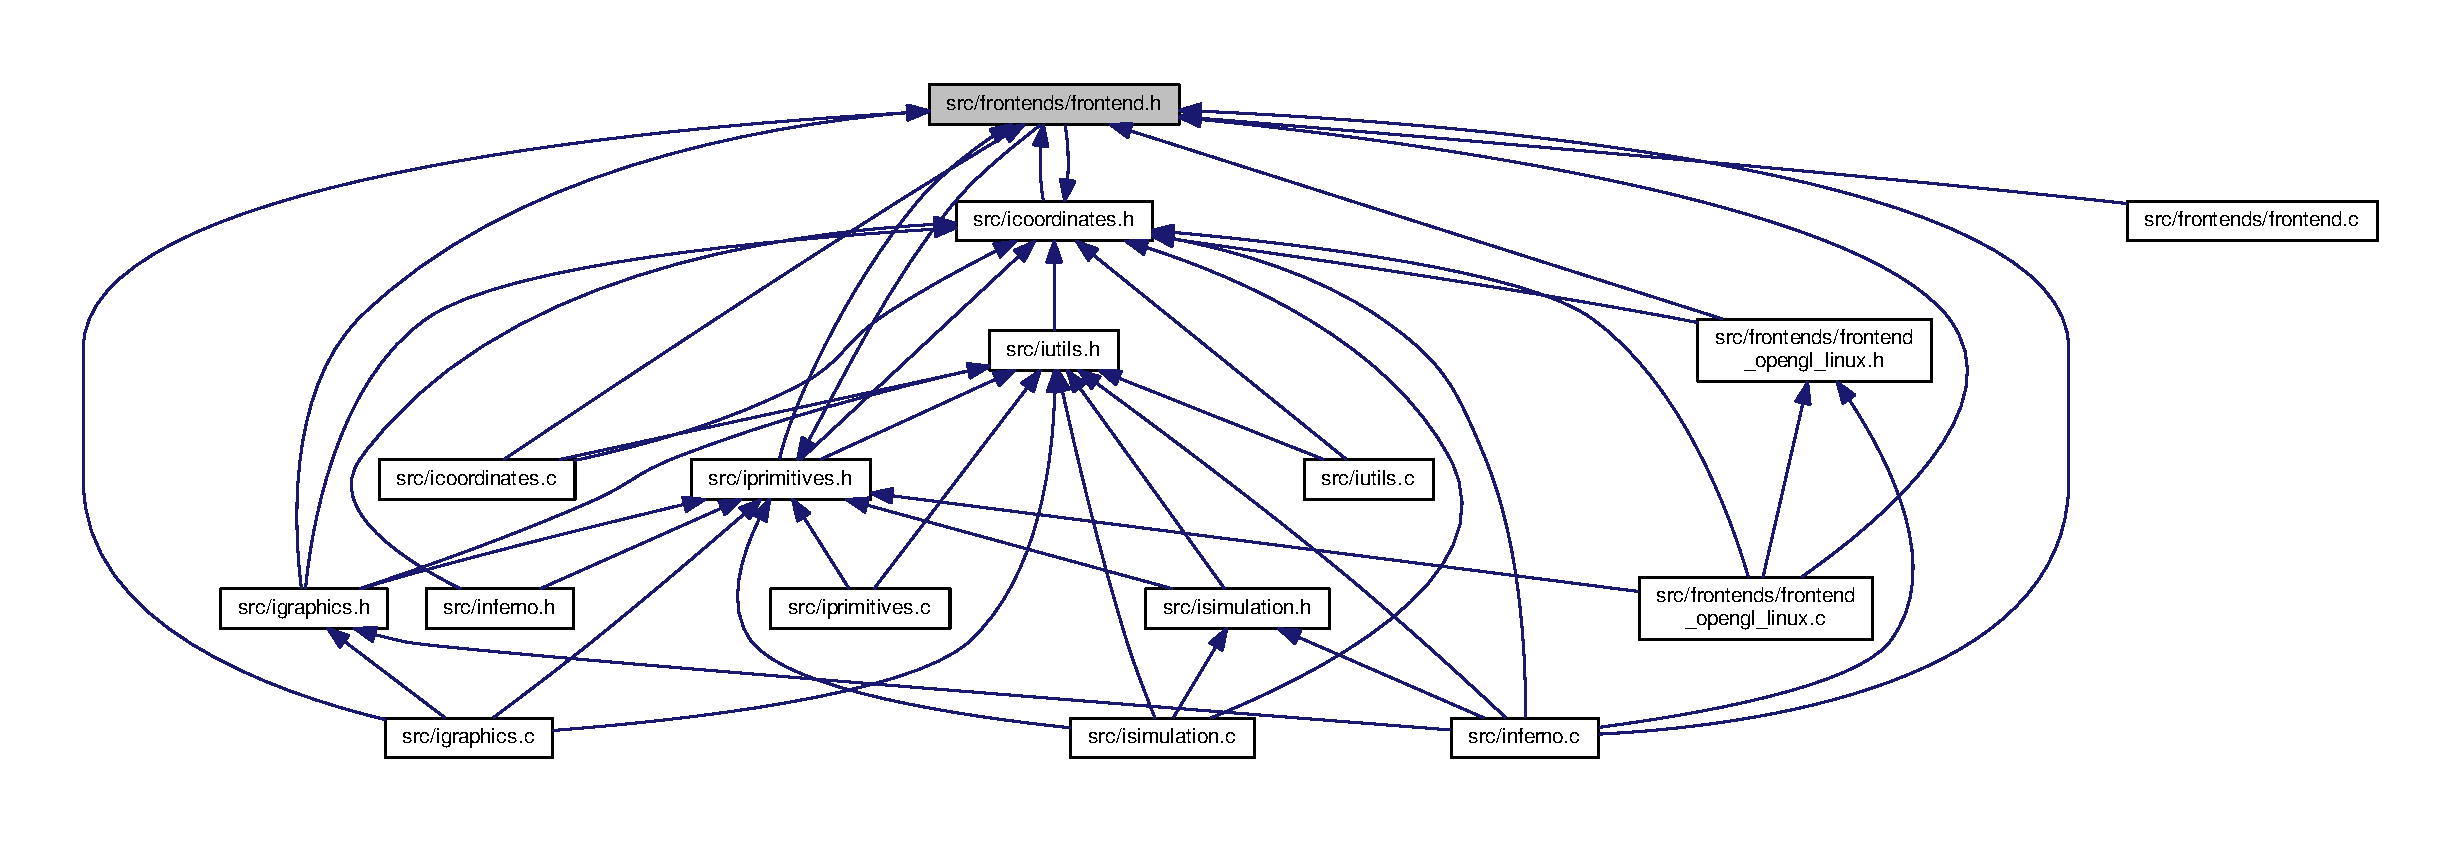
\includegraphics[width=350pt]{frontend_8h__dep__incl}
\end{center}
\end{figure}
\subsection*{Data Structures}
\begin{DoxyCompactItemize}
\item 
struct \hyperlink{structievent__handler}{ievent\-\_\-handler}
\item 
struct \hyperlink{structifrontendstate__t}{ifrontendstate\-\_\-t}
\end{DoxyCompactItemize}
\subsection*{Functions}
\begin{DoxyCompactItemize}
\item 
struct \hyperlink{structievent__handler}{ievent\-\_\-handler} $\ast$ \hyperlink{frontend_8h_af20744b431ee1afa0043f15e5e2f9207}{inew\-\_\-eventhandler} (void $\ast$($\ast$handler)(void $\ast$args, void $\ast$event), void $\ast$args, unsigned short key\-\_\-code)
\item 
void \hyperlink{frontend_8h_a4cb194a7e9456fffef751e2a311735eb}{frontend\-\_\-initialize} ()
\item 
void \hyperlink{frontend_8h_a3012f53c007b67ba7dedf3156eb37e80}{frontend\-\_\-set\-\_\-eventhandler} (unsigned short i, char down, struct \hyperlink{structievent__handler}{ievent\-\_\-handler} $\ast$h, struct \hyperlink{structifrontendstate__t}{ifrontendstate\-\_\-t} $\ast$state)
\item 
void \hyperlink{frontend_8h_aeac975aee6becbb83f7fac162d290fe0}{frontend\-\_\-initialize\-\_\-viewspace} (float x1, float x2, float y1, float y2, int num\-\_\-z\-\_\-levels, struct \hyperlink{structifrontendstate__t}{ifrontendstate\-\_\-t} $\ast$state)
\item 
void \hyperlink{frontend_8h_ad8a729cc49f33a0037227c75e1979ada}{frontend\-\_\-reset\-\_\-viewspace} (struct \hyperlink{structifrontendstate__t}{ifrontendstate\-\_\-t} $\ast$state)
\item 
void \hyperlink{frontend_8h_a5f1d2e26db40b3636fb218810a872a03}{frontend\-\_\-free} ()
\item 
void \hyperlink{frontend_8h_a740fe64ba30a741771700f190e164a9c}{frontend\-\_\-update} (struct \hyperlink{structifrontendstate__t}{ifrontendstate\-\_\-t} $\ast$state)
\item 
void \hyperlink{frontend_8h_a8bf6d9ce46e86be714c47fd5d3a106b8}{frontend\-\_\-draw\-\_\-line} (float x1, float y1, float x2, float y2, struct \hyperlink{structicolor__t}{icolor\-\_\-t} color, int z\-\_\-level)
\item 
void \hyperlink{frontend_8h_a3e3ddec01ee228bbd7e9bce1779e2f74}{frontend\-\_\-draw\-\_\-rectangle} (struct \hyperlink{structipoint__t}{ipoint\-\_\-t} $\ast$p1, struct \hyperlink{structipoint__t}{ipoint\-\_\-t} $\ast$p2, struct \hyperlink{structicolor__t}{icolor\-\_\-t} color)
\item 
void \hyperlink{frontend_8h_a532cd8517ad651db90c6e979addebf82}{frontend\-\_\-draw\-\_\-point} (struct \hyperlink{structipoint__t}{ipoint\-\_\-t} $\ast$point, struct \hyperlink{structicolor__t}{icolor\-\_\-t} color)
\item 
void \hyperlink{frontend_8h_a0443993e9b09570d3b9ab2a6353be8c0}{frontend\-\_\-draw\-\_\-coloredtriplet} (struct \hyperlink{structicoloredtriplet__t}{icoloredtriplet\-\_\-t} $\ast$triplet)
\item 
int \hyperlink{frontend_8h_a6452a9d7c9fcabeb40bb5d8495300090}{step} ()
\end{DoxyCompactItemize}


\subsection{Function Documentation}
\hypertarget{frontend_8h_a0443993e9b09570d3b9ab2a6353be8c0}{\index{frontend.\-h@{frontend.\-h}!frontend\-\_\-draw\-\_\-coloredtriplet@{frontend\-\_\-draw\-\_\-coloredtriplet}}
\index{frontend\-\_\-draw\-\_\-coloredtriplet@{frontend\-\_\-draw\-\_\-coloredtriplet}!frontend.h@{frontend.\-h}}
\subsubsection[{frontend\-\_\-draw\-\_\-coloredtriplet}]{\setlength{\rightskip}{0pt plus 5cm}void frontend\-\_\-draw\-\_\-coloredtriplet (
\begin{DoxyParamCaption}
\item[{struct {\bf icoloredtriplet\-\_\-t} $\ast$}]{triplet}
\end{DoxyParamCaption}
)}}\label{frontend_8h_a0443993e9b09570d3b9ab2a6353be8c0}


Definition at line 149 of file frontend\-\_\-opengl\-\_\-linux.\-c.


\begin{DoxyCode}
150 \{
151         glBegin(GL\_TRIANGLES);
152                 glColor3ub((triplet->\hyperlink{structicoloredtriplet__t_ac0ba48c5e0ba663bd8c0fb7b3ac2a2a9}{colors}[0]->\hyperlink{structicolor__t_af41be99aa200064979c76e29d00d4aff}{r}),
153                           (triplet->\hyperlink{structicoloredtriplet__t_ac0ba48c5e0ba663bd8c0fb7b3ac2a2a9}{colors}[0]->\hyperlink{structicolor__t_a3cf0a9335bbc32fc211d22f3ef502110}{g}),
154                           (triplet->\hyperlink{structicoloredtriplet__t_ac0ba48c5e0ba663bd8c0fb7b3ac2a2a9}{colors}[0]->\hyperlink{structicolor__t_acb75f6cdb4866b33921bde0c5f9000ce}{b}));
155                 glVertex3f(triplet->\hyperlink{structicoloredtriplet__t_aa599939c78c387bc80a763f3e3728fee}{vertices}[0]->\hyperlink{structipoint__t_a345608e139b0709cc281139e3ed6328d}{x}, triplet->\hyperlink{structicoloredtriplet__t_aa599939c78c387bc80a763f3e3728fee}{vertices}[0]->
      \hyperlink{structipoint__t_a88ca543f1508de060b4738cfebb51b04}{y},
156                            (\textcolor{keywordtype}{float})triplet->\hyperlink{structicoloredtriplet__t_aa599939c78c387bc80a763f3e3728fee}{vertices}[0]->\hyperlink{structipoint__t_ad1680bc07190dabf544e86824b82e44b}{z});
157                 glColor3ub(triplet->\hyperlink{structicoloredtriplet__t_ac0ba48c5e0ba663bd8c0fb7b3ac2a2a9}{colors}[1]->\hyperlink{structicolor__t_af41be99aa200064979c76e29d00d4aff}{r},
158                           triplet->\hyperlink{structicoloredtriplet__t_ac0ba48c5e0ba663bd8c0fb7b3ac2a2a9}{colors}[1]->\hyperlink{structicolor__t_a3cf0a9335bbc32fc211d22f3ef502110}{g},
159                           triplet->\hyperlink{structicoloredtriplet__t_ac0ba48c5e0ba663bd8c0fb7b3ac2a2a9}{colors}[1]->\hyperlink{structicolor__t_acb75f6cdb4866b33921bde0c5f9000ce}{b});
160                 glVertex3f(triplet->\hyperlink{structicoloredtriplet__t_aa599939c78c387bc80a763f3e3728fee}{vertices}[1]->\hyperlink{structipoint__t_a345608e139b0709cc281139e3ed6328d}{x}, triplet->\hyperlink{structicoloredtriplet__t_aa599939c78c387bc80a763f3e3728fee}{vertices}[1]->
      \hyperlink{structipoint__t_a88ca543f1508de060b4738cfebb51b04}{y},
161                            (\textcolor{keywordtype}{float})triplet->\hyperlink{structicoloredtriplet__t_aa599939c78c387bc80a763f3e3728fee}{vertices}[1]->\hyperlink{structipoint__t_ad1680bc07190dabf544e86824b82e44b}{z});
162                 glColor3ub(triplet->\hyperlink{structicoloredtriplet__t_ac0ba48c5e0ba663bd8c0fb7b3ac2a2a9}{colors}[2]->\hyperlink{structicolor__t_af41be99aa200064979c76e29d00d4aff}{r},
163                           triplet->\hyperlink{structicoloredtriplet__t_ac0ba48c5e0ba663bd8c0fb7b3ac2a2a9}{colors}[2]->\hyperlink{structicolor__t_a3cf0a9335bbc32fc211d22f3ef502110}{g},
164                           triplet->\hyperlink{structicoloredtriplet__t_ac0ba48c5e0ba663bd8c0fb7b3ac2a2a9}{colors}[2]->\hyperlink{structicolor__t_acb75f6cdb4866b33921bde0c5f9000ce}{b});
165                 glVertex3f(triplet->\hyperlink{structicoloredtriplet__t_aa599939c78c387bc80a763f3e3728fee}{vertices}[2]->\hyperlink{structipoint__t_a345608e139b0709cc281139e3ed6328d}{x}, triplet->\hyperlink{structicoloredtriplet__t_aa599939c78c387bc80a763f3e3728fee}{vertices}[2]->
      \hyperlink{structipoint__t_a88ca543f1508de060b4738cfebb51b04}{y},
166                            (\textcolor{keywordtype}{float})triplet->\hyperlink{structicoloredtriplet__t_aa599939c78c387bc80a763f3e3728fee}{vertices}[2]->\hyperlink{structipoint__t_ad1680bc07190dabf544e86824b82e44b}{z});
167         glEnd();
168 \}
\end{DoxyCode}


Here is the caller graph for this function\-:\nopagebreak
\begin{figure}[H]
\begin{center}
\leavevmode
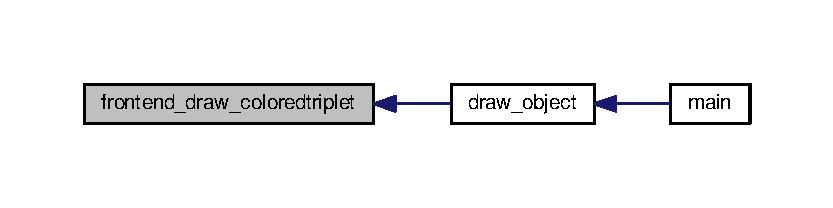
\includegraphics[width=350pt]{frontend_8h_a0443993e9b09570d3b9ab2a6353be8c0_icgraph}
\end{center}
\end{figure}


\hypertarget{frontend_8h_a8bf6d9ce46e86be714c47fd5d3a106b8}{\index{frontend.\-h@{frontend.\-h}!frontend\-\_\-draw\-\_\-line@{frontend\-\_\-draw\-\_\-line}}
\index{frontend\-\_\-draw\-\_\-line@{frontend\-\_\-draw\-\_\-line}!frontend.h@{frontend.\-h}}
\subsubsection[{frontend\-\_\-draw\-\_\-line}]{\setlength{\rightskip}{0pt plus 5cm}void frontend\-\_\-draw\-\_\-line (
\begin{DoxyParamCaption}
\item[{float}]{x1, }
\item[{float}]{y1, }
\item[{float}]{x2, }
\item[{float}]{y2, }
\item[{struct {\bf icolor\-\_\-t}}]{color, }
\item[{int}]{z\-\_\-level}
\end{DoxyParamCaption}
)}}\label{frontend_8h_a8bf6d9ce46e86be714c47fd5d3a106b8}
\hypertarget{frontend_8h_a532cd8517ad651db90c6e979addebf82}{\index{frontend.\-h@{frontend.\-h}!frontend\-\_\-draw\-\_\-point@{frontend\-\_\-draw\-\_\-point}}
\index{frontend\-\_\-draw\-\_\-point@{frontend\-\_\-draw\-\_\-point}!frontend.h@{frontend.\-h}}
\subsubsection[{frontend\-\_\-draw\-\_\-point}]{\setlength{\rightskip}{0pt plus 5cm}void frontend\-\_\-draw\-\_\-point (
\begin{DoxyParamCaption}
\item[{struct {\bf ipoint\-\_\-t} $\ast$}]{point, }
\item[{struct {\bf icolor\-\_\-t}}]{color}
\end{DoxyParamCaption}
)}}\label{frontend_8h_a532cd8517ad651db90c6e979addebf82}


Definition at line 141 of file frontend\-\_\-opengl\-\_\-linux.\-c.


\begin{DoxyCode}
142 \{
143         glBegin(GL\_POINTS);
144                 glColor3f((\textcolor{keywordtype}{float})color.\hyperlink{structicolor__t_af41be99aa200064979c76e29d00d4aff}{r}, (\textcolor{keywordtype}{float})color.\hyperlink{structicolor__t_a3cf0a9335bbc32fc211d22f3ef502110}{g}, (\textcolor{keywordtype}{float})color.\hyperlink{structicolor__t_acb75f6cdb4866b33921bde0c5f9000ce}{b});
145                 glVertex3f(point->\hyperlink{structipoint__t_a345608e139b0709cc281139e3ed6328d}{x}, point->\hyperlink{structipoint__t_a88ca543f1508de060b4738cfebb51b04}{y}, (\textcolor{keywordtype}{float}) point->\hyperlink{structipoint__t_ad1680bc07190dabf544e86824b82e44b}{z});
146         glEnd();
147 \}
\end{DoxyCode}
\hypertarget{frontend_8h_a3e3ddec01ee228bbd7e9bce1779e2f74}{\index{frontend.\-h@{frontend.\-h}!frontend\-\_\-draw\-\_\-rectangle@{frontend\-\_\-draw\-\_\-rectangle}}
\index{frontend\-\_\-draw\-\_\-rectangle@{frontend\-\_\-draw\-\_\-rectangle}!frontend.h@{frontend.\-h}}
\subsubsection[{frontend\-\_\-draw\-\_\-rectangle}]{\setlength{\rightskip}{0pt plus 5cm}void frontend\-\_\-draw\-\_\-rectangle (
\begin{DoxyParamCaption}
\item[{struct {\bf ipoint\-\_\-t} $\ast$}]{p1, }
\item[{struct {\bf ipoint\-\_\-t} $\ast$}]{p2, }
\item[{struct {\bf icolor\-\_\-t}}]{color}
\end{DoxyParamCaption}
)}}\label{frontend_8h_a3e3ddec01ee228bbd7e9bce1779e2f74}


Definition at line 129 of file frontend\-\_\-opengl\-\_\-linux.\-c.


\begin{DoxyCode}
130 \{
131         \textcolor{keywordtype}{float} z = (float) p1->\hyperlink{structipoint__t_ad1680bc07190dabf544e86824b82e44b}{z};
132         glBegin(GL\_QUADS);
133                 glColor3f(color.\hyperlink{structicolor__t_af41be99aa200064979c76e29d00d4aff}{r}, color.\hyperlink{structicolor__t_a3cf0a9335bbc32fc211d22f3ef502110}{g}, color.\hyperlink{structicolor__t_acb75f6cdb4866b33921bde0c5f9000ce}{b});
134                 glVertex3f(p1->\hyperlink{structipoint__t_a345608e139b0709cc281139e3ed6328d}{x}, p1->\hyperlink{structipoint__t_a88ca543f1508de060b4738cfebb51b04}{y}, z);
135                 glVertex3f(p2->\hyperlink{structipoint__t_a345608e139b0709cc281139e3ed6328d}{x}, p1->\hyperlink{structipoint__t_a88ca543f1508de060b4738cfebb51b04}{y}, z);
136                 glVertex3f(p2->\hyperlink{structipoint__t_a345608e139b0709cc281139e3ed6328d}{x}, p2->\hyperlink{structipoint__t_a88ca543f1508de060b4738cfebb51b04}{y}, z);
137                 glVertex3f(p1->\hyperlink{structipoint__t_a345608e139b0709cc281139e3ed6328d}{x}, p2->\hyperlink{structipoint__t_a88ca543f1508de060b4738cfebb51b04}{y}, z);
138         glEnd();
139 \}
\end{DoxyCode}
\hypertarget{frontend_8h_a5f1d2e26db40b3636fb218810a872a03}{\index{frontend.\-h@{frontend.\-h}!frontend\-\_\-free@{frontend\-\_\-free}}
\index{frontend\-\_\-free@{frontend\-\_\-free}!frontend.h@{frontend.\-h}}
\subsubsection[{frontend\-\_\-free}]{\setlength{\rightskip}{0pt plus 5cm}void frontend\-\_\-free (
\begin{DoxyParamCaption}
{}
\end{DoxyParamCaption}
)}}\label{frontend_8h_a5f1d2e26db40b3636fb218810a872a03}


Definition at line 112 of file frontend\-\_\-opengl\-\_\-linux.\-c.


\begin{DoxyCode}
113 \{
114         printf(\textcolor{stringliteral}{"Freeing frontend resources...\(\backslash\)n"});
115         glXMakeCurrent(\hyperlink{frontend__opengl__linux_8h_a7d43b3edf58f8d85a89852ab95b740f6}{dpy}, None, NULL);
116         glXDestroyContext(\hyperlink{frontend__opengl__linux_8h_a7d43b3edf58f8d85a89852ab95b740f6}{dpy}, \hyperlink{frontend__opengl__linux_8h_a865db36501e45073170bee430ee35fc3}{glc});
117         XDestroyWindow(\hyperlink{frontend__opengl__linux_8h_a7d43b3edf58f8d85a89852ab95b740f6}{dpy}, \hyperlink{frontend__opengl__linux_8h_af5e9cbaf11bc8c0c330917f546d0045f}{win});
118         XCloseDisplay(\hyperlink{frontend__opengl__linux_8h_a7d43b3edf58f8d85a89852ab95b740f6}{dpy});
119 \}
\end{DoxyCode}


Here is the caller graph for this function\-:\nopagebreak
\begin{figure}[H]
\begin{center}
\leavevmode
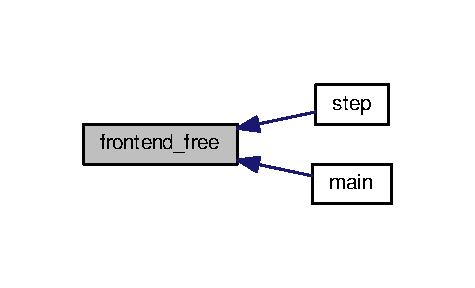
\includegraphics[width=228pt]{frontend_8h_a5f1d2e26db40b3636fb218810a872a03_icgraph}
\end{center}
\end{figure}


\hypertarget{frontend_8h_a4cb194a7e9456fffef751e2a311735eb}{\index{frontend.\-h@{frontend.\-h}!frontend\-\_\-initialize@{frontend\-\_\-initialize}}
\index{frontend\-\_\-initialize@{frontend\-\_\-initialize}!frontend.h@{frontend.\-h}}
\subsubsection[{frontend\-\_\-initialize}]{\setlength{\rightskip}{0pt plus 5cm}void frontend\-\_\-initialize (
\begin{DoxyParamCaption}
{}
\end{DoxyParamCaption}
)}}\label{frontend_8h_a4cb194a7e9456fffef751e2a311735eb}


Definition at line 27 of file frontend\-\_\-opengl\-\_\-linux.\-c.


\begin{DoxyCode}
28 \{
29         \textcolor{comment}{//att = \{ GLX\_RGBA, GLX\_DEPTH\_SIZE, 24, GLX\_DOUBLEBUFFER, None \};}
30         \hyperlink{frontend__opengl__linux_8h_a5222c83ddcc16d2021dab765c97f6955}{att}[0] = GLX\_RGBA;
31         \hyperlink{frontend__opengl__linux_8h_a5222c83ddcc16d2021dab765c97f6955}{att}[1] = GLX\_DEPTH\_SIZE;
32         \hyperlink{frontend__opengl__linux_8h_a5222c83ddcc16d2021dab765c97f6955}{att}[2] = 24;
33         \hyperlink{frontend__opengl__linux_8h_a5222c83ddcc16d2021dab765c97f6955}{att}[3] = GLX\_DOUBLEBUFFER;
34         \hyperlink{frontend__opengl__linux_8h_a5222c83ddcc16d2021dab765c97f6955}{att}[4] = None;
35         \hyperlink{frontend__opengl__linux_8h_a7d43b3edf58f8d85a89852ab95b740f6}{dpy} = XOpenDisplay(NULL);
36         
37         \textcolor{keywordflow}{if}(\hyperlink{frontend__opengl__linux_8h_a7d43b3edf58f8d85a89852ab95b740f6}{dpy} == NULL) \{
38                 printf(\textcolor{stringliteral}{"\(\backslash\)n\(\backslash\)tcannot connect to X server\(\backslash\)n\(\backslash\)n"});
39                 exit(0);
40         \}
41 
42         \hyperlink{frontend__opengl__linux_8h_a67efd2aa4387dcb1b33df1f044512a16}{root} = DefaultRootWindow(\hyperlink{frontend__opengl__linux_8h_a7d43b3edf58f8d85a89852ab95b740f6}{dpy});
43 
44         \hyperlink{frontend__opengl__linux_8h_a6ea38ddc009c6f56a768347fa8cca7fc}{vi} = glXChooseVisual(\hyperlink{frontend__opengl__linux_8h_a7d43b3edf58f8d85a89852ab95b740f6}{dpy}, 0, \hyperlink{frontend__opengl__linux_8h_a5222c83ddcc16d2021dab765c97f6955}{att});
45 
46         \textcolor{keywordflow}{if}(\hyperlink{frontend__opengl__linux_8h_a6ea38ddc009c6f56a768347fa8cca7fc}{vi} == NULL) \{
47                 printf(\textcolor{stringliteral}{"\(\backslash\)n\(\backslash\)tno appropriate visual found\(\backslash\)n\(\backslash\)n"});
48                 exit(0);
49         \} 
50         \textcolor{keywordflow}{else} \{
51                 printf(\textcolor{stringliteral}{"\(\backslash\)n\(\backslash\)tvisual %p selected\(\backslash\)n"}, (\textcolor{keywordtype}{void} *)\hyperlink{frontend__opengl__linux_8h_a6ea38ddc009c6f56a768347fa8cca7fc}{vi}->visualid);
52         \}
53 
54         \hyperlink{frontend__opengl__linux_8h_ae9e16ee22daffbbbbf59f6c841c2ab75}{cmap} = XCreateColormap(\hyperlink{frontend__opengl__linux_8h_a7d43b3edf58f8d85a89852ab95b740f6}{dpy}, \hyperlink{frontend__opengl__linux_8h_a67efd2aa4387dcb1b33df1f044512a16}{root}, \hyperlink{frontend__opengl__linux_8h_a6ea38ddc009c6f56a768347fa8cca7fc}{vi}->visual, AllocNone);
55 
56         \hyperlink{frontend__opengl__linux_8h_a89fc0a57cdcd1daf998256dd0f62acd2}{swa}.colormap = \hyperlink{frontend__opengl__linux_8h_ae9e16ee22daffbbbbf59f6c841c2ab75}{cmap};
57         \hyperlink{frontend__opengl__linux_8h_a89fc0a57cdcd1daf998256dd0f62acd2}{swa}.event\_mask = ExposureMask | KeyPressMask;
58 
59         \hyperlink{frontend__opengl__linux_8h_af5e9cbaf11bc8c0c330917f546d0045f}{win} = XCreateWindow(\hyperlink{frontend__opengl__linux_8h_a7d43b3edf58f8d85a89852ab95b740f6}{dpy}, \hyperlink{frontend__opengl__linux_8h_a67efd2aa4387dcb1b33df1f044512a16}{root}, 0, 0, 600, 600, 0,
60                                 \hyperlink{frontend__opengl__linux_8h_a6ea38ddc009c6f56a768347fa8cca7fc}{vi}->depth, InputOutput, \hyperlink{frontend__opengl__linux_8h_a6ea38ddc009c6f56a768347fa8cca7fc}{vi}->visual,
61                                 CWColormap | CWEventMask, &\hyperlink{frontend__opengl__linux_8h_a89fc0a57cdcd1daf998256dd0f62acd2}{swa});
62 
63         XMapWindow(\hyperlink{frontend__opengl__linux_8h_a7d43b3edf58f8d85a89852ab95b740f6}{dpy}, \hyperlink{frontend__opengl__linux_8h_af5e9cbaf11bc8c0c330917f546d0045f}{win});
64 
65         XStoreName(\hyperlink{frontend__opengl__linux_8h_a7d43b3edf58f8d85a89852ab95b740f6}{dpy}, \hyperlink{frontend__opengl__linux_8h_af5e9cbaf11bc8c0c330917f546d0045f}{win}, \textcolor{stringliteral}{"VERY SIMPLE APPLICATION"});
66 
67         \hyperlink{frontend__opengl__linux_8h_a865db36501e45073170bee430ee35fc3}{glc} = glXCreateContext(\hyperlink{frontend__opengl__linux_8h_a7d43b3edf58f8d85a89852ab95b740f6}{dpy}, \hyperlink{frontend__opengl__linux_8h_a6ea38ddc009c6f56a768347fa8cca7fc}{vi}, NULL, GL\_TRUE);
68         glXMakeCurrent(\hyperlink{frontend__opengl__linux_8h_a7d43b3edf58f8d85a89852ab95b740f6}{dpy}, \hyperlink{frontend__opengl__linux_8h_af5e9cbaf11bc8c0c330917f546d0045f}{win}, \hyperlink{frontend__opengl__linux_8h_a865db36501e45073170bee430ee35fc3}{glc});
69 
70         glDisable(GL\_DEPTH\_TEST);
71 \}
\end{DoxyCode}


Here is the caller graph for this function\-:\nopagebreak
\begin{figure}[H]
\begin{center}
\leavevmode
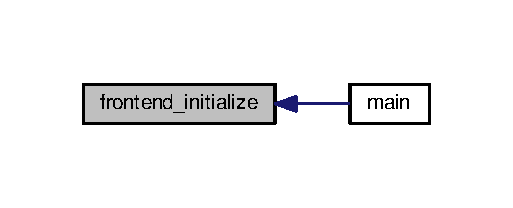
\includegraphics[width=246pt]{frontend_8h_a4cb194a7e9456fffef751e2a311735eb_icgraph}
\end{center}
\end{figure}


\hypertarget{frontend_8h_aeac975aee6becbb83f7fac162d290fe0}{\index{frontend.\-h@{frontend.\-h}!frontend\-\_\-initialize\-\_\-viewspace@{frontend\-\_\-initialize\-\_\-viewspace}}
\index{frontend\-\_\-initialize\-\_\-viewspace@{frontend\-\_\-initialize\-\_\-viewspace}!frontend.h@{frontend.\-h}}
\subsubsection[{frontend\-\_\-initialize\-\_\-viewspace}]{\setlength{\rightskip}{0pt plus 5cm}void frontend\-\_\-initialize\-\_\-viewspace (
\begin{DoxyParamCaption}
\item[{float}]{x1, }
\item[{float}]{x2, }
\item[{float}]{y1, }
\item[{float}]{y2, }
\item[{int}]{num\-\_\-z\-\_\-levels, }
\item[{struct {\bf ifrontendstate\-\_\-t} $\ast$}]{state}
\end{DoxyParamCaption}
)}}\label{frontend_8h_aeac975aee6becbb83f7fac162d290fe0}
\begin{DoxyReturn}{Returns}
a bitmap with the 0 byte being the number of \char`\"{}near\char`\"{} z-\/levels and the 1 byte being the number of \char`\"{}far\char`\"{} z-\/levels 
\end{DoxyReturn}


Definition at line 76 of file frontend\-\_\-opengl\-\_\-linux.\-c.


\begin{DoxyCode}
77 \{
78         state->\hyperlink{structifrontendstate__t_afb7c49000e593f77bcb30b1ae4384ded}{background\_color} = malloc(\textcolor{keyword}{sizeof}(\textcolor{keyword}{struct} \hyperlink{structicolor__t}{icolor\_t}));
79         state->\hyperlink{structifrontendstate__t_ac81d750ec8cd1ba1d44e2c0f55bea687}{drawing\_color} = malloc(\textcolor{keyword}{sizeof}(\textcolor{keyword}{struct} \hyperlink{structicolor__t}{icolor\_t}));
80         state->\hyperlink{structifrontendstate__t_a54ee910059c66c18fa1bb1555d0e61c5}{left} = x1;
81         state->\hyperlink{structifrontendstate__t_a7c304035e472522fb01b3bb85b37eef8}{right} = x2;
82         state->\hyperlink{structifrontendstate__t_adc025993349dceae53dfe235f84fdef2}{bottom} = y1;
83         state->\hyperlink{structifrontendstate__t_afda9cb91a47174c6e95a4888918964f4}{top} = y2;
84         state->\hyperlink{structifrontendstate__t_aefb96a4cd8758bcd9a3e5b506290adca}{z\_levels} = num\_z\_levels;
85         state->\hyperlink{structifrontendstate__t_ad30593dd0b69372008108075c55cfe27}{num\_regions} = 0;
86         state->\hyperlink{structifrontendstate__t_a42ce77321ecea4fde68dd68b7f0f2283}{regions} = NULL;
87         \hyperlink{icoordinates_8c_a4507e51c1f2470e19e8ff5a77adf54bd}{icreate\_region}(0, 0, 100, 100, state);
88         \textcolor{keywordtype}{int} i;
89         \textcolor{keywordflow}{for} (i = 0; i < 256; i++) \{
90                 state->\hyperlink{structifrontendstate__t_a5bb9423c4ba5f86cd8a0d50575031952}{onkeyup\_handlers}[i]   = \hyperlink{frontend_8c_af20744b431ee1afa0043f15e5e2f9207}{inew\_eventhandler}(NULL, 
      NULL, i);
91                 state->\hyperlink{structifrontendstate__t_ad8fd468eaec37b949af562b39ad20d5a}{onkeydown\_handlers}[i] = 
      \hyperlink{frontend_8c_af20744b431ee1afa0043f15e5e2f9207}{inew\_eventhandler}(NULL, NULL, i);
92         \}
93 \}
\end{DoxyCode}


Here is the call graph for this function\-:\nopagebreak
\begin{figure}[H]
\begin{center}
\leavevmode
\includegraphics[width=350pt]{frontend_8h_aeac975aee6becbb83f7fac162d290fe0_cgraph}
\end{center}
\end{figure}




Here is the caller graph for this function\-:\nopagebreak
\begin{figure}[H]
\begin{center}
\leavevmode
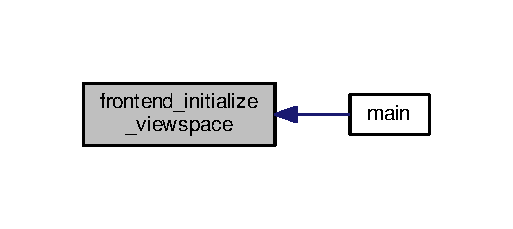
\includegraphics[width=246pt]{frontend_8h_aeac975aee6becbb83f7fac162d290fe0_icgraph}
\end{center}
\end{figure}


\hypertarget{frontend_8h_ad8a729cc49f33a0037227c75e1979ada}{\index{frontend.\-h@{frontend.\-h}!frontend\-\_\-reset\-\_\-viewspace@{frontend\-\_\-reset\-\_\-viewspace}}
\index{frontend\-\_\-reset\-\_\-viewspace@{frontend\-\_\-reset\-\_\-viewspace}!frontend.h@{frontend.\-h}}
\subsubsection[{frontend\-\_\-reset\-\_\-viewspace}]{\setlength{\rightskip}{0pt plus 5cm}void frontend\-\_\-reset\-\_\-viewspace (
\begin{DoxyParamCaption}
\item[{struct {\bf ifrontendstate\-\_\-t} $\ast$}]{state}
\end{DoxyParamCaption}
)}}\label{frontend_8h_ad8a729cc49f33a0037227c75e1979ada}


Definition at line 95 of file frontend\-\_\-opengl\-\_\-linux.\-c.


\begin{DoxyCode}
96 \{
97         glClearColor((\textcolor{keywordtype}{float})\hyperlink{iprimitives_8c_afc34677b05531522408374dc02a31f40}{red}(*state->\hyperlink{structifrontendstate__t_afb7c49000e593f77bcb30b1ae4384ded}{background\_color})/256.,
98                      (\textcolor{keywordtype}{float})\hyperlink{iprimitives_8c_abc6932dd227752af4dbf7fac0b6e3291}{green}(*state->\hyperlink{structifrontendstate__t_afb7c49000e593f77bcb30b1ae4384ded}{background\_color})/256.,
99                      (\textcolor{keywordtype}{float})\hyperlink{iprimitives_8c_a03066bd036a134534caeec08526b7269}{blue}(*state->\hyperlink{structifrontendstate__t_afb7c49000e593f77bcb30b1ae4384ded}{background\_color})/256., 1.0);
100         glClear(GL\_COLOR\_BUFFER\_BIT | GL\_DEPTH\_BUFFER\_BIT);
101 
102         glMatrixMode(GL\_PROJECTION);
103         glLoadIdentity();
104         glOrtho(state->\hyperlink{structifrontendstate__t_a54ee910059c66c18fa1bb1555d0e61c5}{left}, state->\hyperlink{structifrontendstate__t_a7c304035e472522fb01b3bb85b37eef8}{right}, state->\hyperlink{structifrontendstate__t_adc025993349dceae53dfe235f84fdef2}{bottom}, state->
      \hyperlink{structifrontendstate__t_afda9cb91a47174c6e95a4888918964f4}{top}, state->\hyperlink{structifrontendstate__t_aefb96a4cd8758bcd9a3e5b506290adca}{z\_levels}, 0);
105 
106         glMatrixMode(GL\_MODELVIEW);
107         glLoadIdentity();
108         gluLookAt(0., 0., 10., 0., 0., 0., 0., 1., 0.);
109 \}
\end{DoxyCode}


Here is the call graph for this function\-:\nopagebreak
\begin{figure}[H]
\begin{center}
\leavevmode
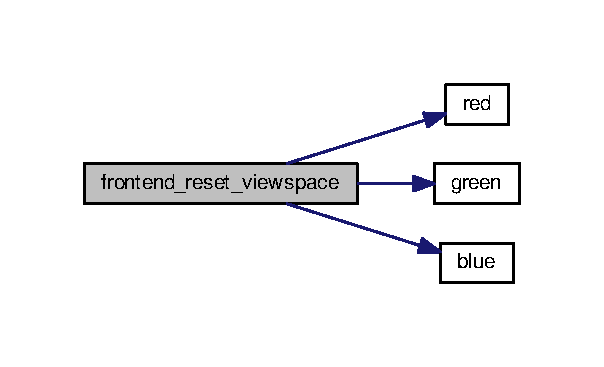
\includegraphics[width=290pt]{frontend_8h_ad8a729cc49f33a0037227c75e1979ada_cgraph}
\end{center}
\end{figure}




Here is the caller graph for this function\-:\nopagebreak
\begin{figure}[H]
\begin{center}
\leavevmode
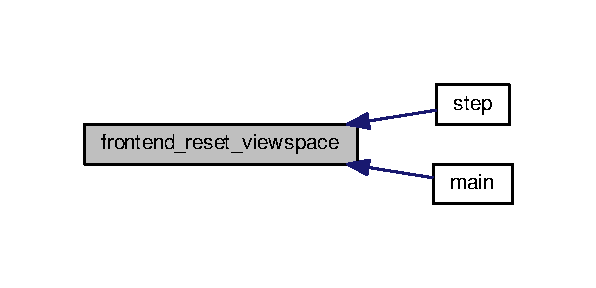
\includegraphics[width=286pt]{frontend_8h_ad8a729cc49f33a0037227c75e1979ada_icgraph}
\end{center}
\end{figure}


\hypertarget{frontend_8h_a3012f53c007b67ba7dedf3156eb37e80}{\index{frontend.\-h@{frontend.\-h}!frontend\-\_\-set\-\_\-eventhandler@{frontend\-\_\-set\-\_\-eventhandler}}
\index{frontend\-\_\-set\-\_\-eventhandler@{frontend\-\_\-set\-\_\-eventhandler}!frontend.h@{frontend.\-h}}
\subsubsection[{frontend\-\_\-set\-\_\-eventhandler}]{\setlength{\rightskip}{0pt plus 5cm}void frontend\-\_\-set\-\_\-eventhandler (
\begin{DoxyParamCaption}
\item[{unsigned short}]{i, }
\item[{char}]{down, }
\item[{struct {\bf ievent\-\_\-handler} $\ast$}]{h, }
\item[{struct {\bf ifrontendstate\-\_\-t} $\ast$}]{state}
\end{DoxyParamCaption}
)}}\label{frontend_8h_a3012f53c007b67ba7dedf3156eb37e80}


Definition at line 31 of file frontend.\-c.


\begin{DoxyCode}
32 \{
33         \textcolor{keywordflow}{if} (down)
34                 state->\hyperlink{structifrontendstate__t_ad8fd468eaec37b949af562b39ad20d5a}{onkeydown\_handlers}[i] = h;
35         \textcolor{keywordflow}{else}
36                 state->\hyperlink{structifrontendstate__t_a5bb9423c4ba5f86cd8a0d50575031952}{onkeyup\_handlers}[i] = h;
37 \}
\end{DoxyCode}


Here is the caller graph for this function\-:\nopagebreak
\begin{figure}[H]
\begin{center}
\leavevmode
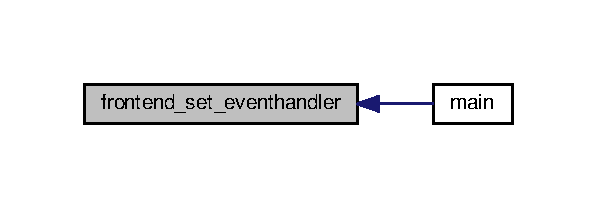
\includegraphics[width=286pt]{frontend_8h_a3012f53c007b67ba7dedf3156eb37e80_icgraph}
\end{center}
\end{figure}


\hypertarget{frontend_8h_a740fe64ba30a741771700f190e164a9c}{\index{frontend.\-h@{frontend.\-h}!frontend\-\_\-update@{frontend\-\_\-update}}
\index{frontend\-\_\-update@{frontend\-\_\-update}!frontend.h@{frontend.\-h}}
\subsubsection[{frontend\-\_\-update}]{\setlength{\rightskip}{0pt plus 5cm}void frontend\-\_\-update (
\begin{DoxyParamCaption}
\item[{struct {\bf ifrontendstate\-\_\-t} $\ast$}]{state}
\end{DoxyParamCaption}
)}}\label{frontend_8h_a740fe64ba30a741771700f190e164a9c}


Definition at line 121 of file frontend\-\_\-opengl\-\_\-linux.\-c.


\begin{DoxyCode}
122 \{
123         XGetWindowAttributes(\hyperlink{frontend__opengl__linux_8h_a7d43b3edf58f8d85a89852ab95b740f6}{dpy}, \hyperlink{frontend__opengl__linux_8h_af5e9cbaf11bc8c0c330917f546d0045f}{win}, &\hyperlink{frontend__opengl__linux_8h_aba75c5c2ba56afc9f1960cb36460d247}{gwa});
124         glViewport(0, 0, \hyperlink{frontend__opengl__linux_8h_aba75c5c2ba56afc9f1960cb36460d247}{gwa}.width, \hyperlink{frontend__opengl__linux_8h_aba75c5c2ba56afc9f1960cb36460d247}{gwa}.height);
125         \textcolor{comment}{//DrawAQuad(); }
126         glXSwapBuffers(\hyperlink{frontend__opengl__linux_8h_a7d43b3edf58f8d85a89852ab95b740f6}{dpy}, \hyperlink{frontend__opengl__linux_8h_af5e9cbaf11bc8c0c330917f546d0045f}{win});
127 \}
\end{DoxyCode}


Here is the caller graph for this function\-:\nopagebreak
\begin{figure}[H]
\begin{center}
\leavevmode
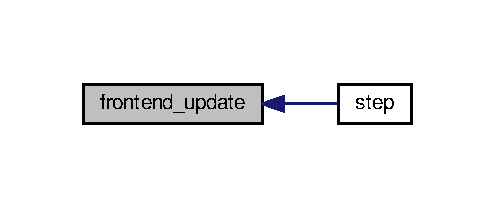
\includegraphics[width=238pt]{frontend_8h_a740fe64ba30a741771700f190e164a9c_icgraph}
\end{center}
\end{figure}


\hypertarget{frontend_8h_af20744b431ee1afa0043f15e5e2f9207}{\index{frontend.\-h@{frontend.\-h}!inew\-\_\-eventhandler@{inew\-\_\-eventhandler}}
\index{inew\-\_\-eventhandler@{inew\-\_\-eventhandler}!frontend.h@{frontend.\-h}}
\subsubsection[{inew\-\_\-eventhandler}]{\setlength{\rightskip}{0pt plus 5cm}struct {\bf ievent\-\_\-handler}$\ast$ inew\-\_\-eventhandler (
\begin{DoxyParamCaption}
\item[{void $\ast$($\ast$)(void $\ast$args, void $\ast$event)}]{handler, }
\item[{void $\ast$}]{args, }
\item[{unsigned short}]{key\-\_\-code}
\end{DoxyParamCaption}
)}}\label{frontend_8h_af20744b431ee1afa0043f15e5e2f9207}


Definition at line 22 of file frontend.\-c.


\begin{DoxyCode}
23 \{
24         \textcolor{keyword}{struct }\hyperlink{structievent__handler}{ievent\_handler} *rval = malloc(\textcolor{keyword}{sizeof}(\textcolor{keyword}{struct} 
      \hyperlink{structievent__handler}{ievent\_handler}));
25         rval->\hyperlink{structievent__handler_a320eaffc01d119279ead9c5ad877c6da}{handler} = \hyperlink{structievent__handler_a320eaffc01d119279ead9c5ad877c6da}{handler};
26         rval->\hyperlink{structievent__handler_ac6b4e6b5b95ada7b0d9985f738ffe1e5}{args} = \hyperlink{structievent__handler_ac6b4e6b5b95ada7b0d9985f738ffe1e5}{args};
27         rval->\hyperlink{structievent__handler_af2766b148965989b8d202b11b9e72f60}{key\_code} = \hyperlink{structievent__handler_af2766b148965989b8d202b11b9e72f60}{key\_code};
28         \textcolor{keywordflow}{return} rval;
29 \}
\end{DoxyCode}


Here is the caller graph for this function\-:\nopagebreak
\begin{figure}[H]
\begin{center}
\leavevmode
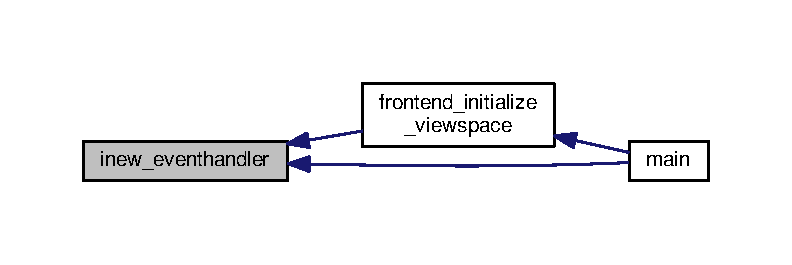
\includegraphics[width=350pt]{frontend_8h_af20744b431ee1afa0043f15e5e2f9207_icgraph}
\end{center}
\end{figure}


\hypertarget{frontend_8h_a6452a9d7c9fcabeb40bb5d8495300090}{\index{frontend.\-h@{frontend.\-h}!step@{step}}
\index{step@{step}!frontend.h@{frontend.\-h}}
\subsubsection[{step}]{\setlength{\rightskip}{0pt plus 5cm}int step (
\begin{DoxyParamCaption}
{}
\end{DoxyParamCaption}
)}}\label{frontend_8h_a6452a9d7c9fcabeb40bb5d8495300090}


Here is the caller graph for this function\-:\nopagebreak
\begin{figure}[H]
\begin{center}
\leavevmode
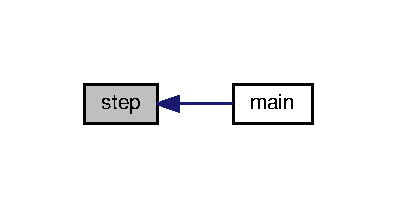
\includegraphics[width=190pt]{frontend_8h_a6452a9d7c9fcabeb40bb5d8495300090_icgraph}
\end{center}
\end{figure}



\hypertarget{frontend__opengl__linux_8c}{\section{src/frontends/frontend\-\_\-opengl\-\_\-linux.c File Reference}
\label{frontend__opengl__linux_8c}\index{src/frontends/frontend\-\_\-opengl\-\_\-linux.\-c@{src/frontends/frontend\-\_\-opengl\-\_\-linux.\-c}}
}
{\ttfamily \#include $<$stdio.\-h$>$}\\*
{\ttfamily \#include $<$stdlib.\-h$>$}\\*
{\ttfamily \#include $<$X11/\-X.\-h$>$}\\*
{\ttfamily \#include $<$X11/\-Xlib.\-h$>$}\\*
{\ttfamily \#include $<$G\-L/gl.\-h$>$}\\*
{\ttfamily \#include $<$G\-L/glx.\-h$>$}\\*
{\ttfamily \#include $<$G\-L/glu.\-h$>$}\\*
{\ttfamily \#include \char`\"{}frontend.\-h\char`\"{}}\\*
{\ttfamily \#include \char`\"{}../icoordinates.\-h\char`\"{}}\\*
{\ttfamily \#include \char`\"{}frontend\-\_\-opengl\-\_\-linux.\-h\char`\"{}}\\*
{\ttfamily \#include \char`\"{}../iprimitives.\-h\char`\"{}}\\*
Include dependency graph for frontend\-\_\-opengl\-\_\-linux.\-c\-:\nopagebreak
\begin{figure}[H]
\begin{center}
\leavevmode
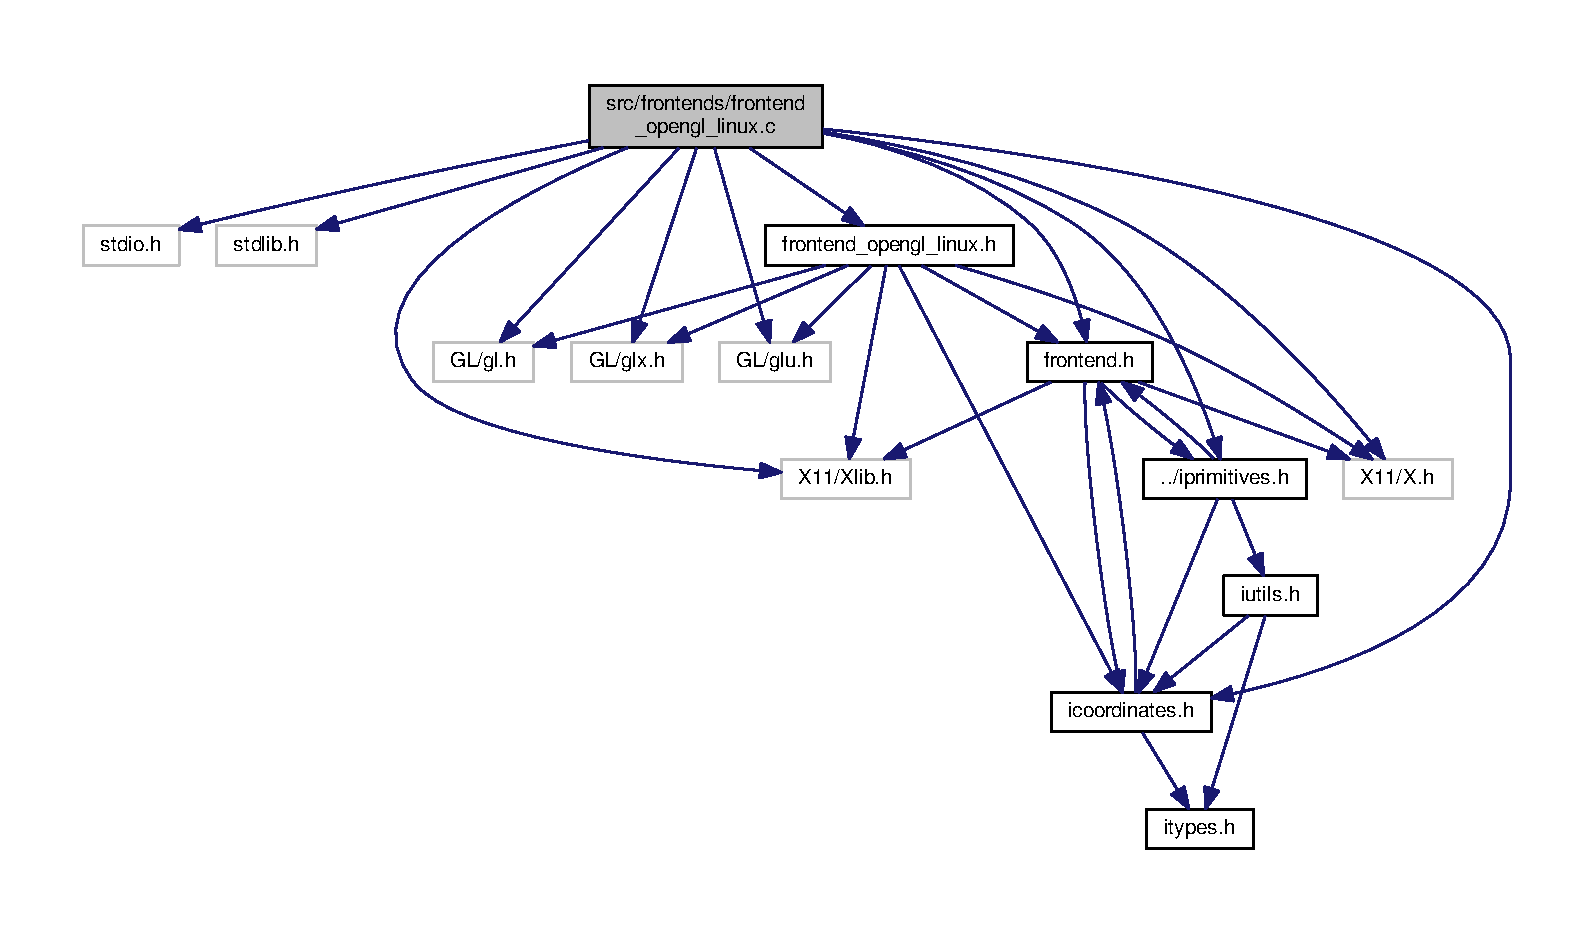
\includegraphics[width=350pt]{frontend__opengl__linux_8c__incl}
\end{center}
\end{figure}
\subsection*{Functions}
\begin{DoxyCompactItemize}
\item 
void \hyperlink{frontend__opengl__linux_8c_a345706a31501f213b1c7ad1825d4628f}{Draw\-A\-Quad} ()
\item 
void \hyperlink{frontend__opengl__linux_8c_a4cb194a7e9456fffef751e2a311735eb}{frontend\-\_\-initialize} ()
\item 
void \hyperlink{frontend__opengl__linux_8c_aeac975aee6becbb83f7fac162d290fe0}{frontend\-\_\-initialize\-\_\-viewspace} (float x1, float x2, float y1, float y2, int num\-\_\-z\-\_\-levels, struct \hyperlink{structifrontendstate__t}{ifrontendstate\-\_\-t} $\ast$state)
\item 
void \hyperlink{frontend__opengl__linux_8c_ad8a729cc49f33a0037227c75e1979ada}{frontend\-\_\-reset\-\_\-viewspace} (struct \hyperlink{structifrontendstate__t}{ifrontendstate\-\_\-t} $\ast$state)
\item 
void \hyperlink{frontend__opengl__linux_8c_a5f1d2e26db40b3636fb218810a872a03}{frontend\-\_\-free} ()
\item 
void \hyperlink{frontend__opengl__linux_8c_a740fe64ba30a741771700f190e164a9c}{frontend\-\_\-update} (struct \hyperlink{structifrontendstate__t}{ifrontendstate\-\_\-t} $\ast$state)
\item 
void \hyperlink{frontend__opengl__linux_8c_a3e3ddec01ee228bbd7e9bce1779e2f74}{frontend\-\_\-draw\-\_\-rectangle} (struct \hyperlink{structipoint__t}{ipoint\-\_\-t} $\ast$p1, struct \hyperlink{structipoint__t}{ipoint\-\_\-t} $\ast$p2, struct \hyperlink{structicolor__t}{icolor\-\_\-t} color)
\item 
void \hyperlink{frontend__opengl__linux_8c_a532cd8517ad651db90c6e979addebf82}{frontend\-\_\-draw\-\_\-point} (struct \hyperlink{structipoint__t}{ipoint\-\_\-t} $\ast$point, struct \hyperlink{structicolor__t}{icolor\-\_\-t} color)
\item 
void \hyperlink{frontend__opengl__linux_8c_a0443993e9b09570d3b9ab2a6353be8c0}{frontend\-\_\-draw\-\_\-coloredtriplet} (struct \hyperlink{structicoloredtriplet__t}{icoloredtriplet\-\_\-t} $\ast$triplet)
\item 
int \hyperlink{frontend__opengl__linux_8c_a606f78ac8a9bdf59c7a520da2b2052e0}{step} (struct \hyperlink{structifrontendstate__t}{ifrontendstate\-\_\-t} $\ast$state)
\end{DoxyCompactItemize}


\subsection{Function Documentation}
\hypertarget{frontend__opengl__linux_8c_a345706a31501f213b1c7ad1825d4628f}{\index{frontend\-\_\-opengl\-\_\-linux.\-c@{frontend\-\_\-opengl\-\_\-linux.\-c}!Draw\-A\-Quad@{Draw\-A\-Quad}}
\index{Draw\-A\-Quad@{Draw\-A\-Quad}!frontend_opengl_linux.c@{frontend\-\_\-opengl\-\_\-linux.\-c}}
\subsubsection[{Draw\-A\-Quad}]{\setlength{\rightskip}{0pt plus 5cm}void Draw\-A\-Quad (
\begin{DoxyParamCaption}
{}
\end{DoxyParamCaption}
)}}\label{frontend__opengl__linux_8c_a345706a31501f213b1c7ad1825d4628f}


Definition at line 16 of file frontend\-\_\-opengl\-\_\-linux.\-c.


\begin{DoxyCode}
16                  \{
17         glBegin(GL\_QUADS);
18         \textcolor{comment}{/*glColor3f(1., 0., 0.); glVertex3f(-.75, -.75, 0.);}
19 \textcolor{comment}{        glColor3f(0., 1., 0.); glVertex3f( 75, -.75, 0.);}
20 \textcolor{comment}{        glColor3f(0., 0., 1.); glVertex3f( .75,  .75, 0.);}
21 \textcolor{comment}{        glColor3f(1., 1., 0.); glVertex3f(-.75,  .75, 0.);*/}
22         glColor3f(0., 0., 0.);
23         glVertex2f(0.0, 0.); glVertex2f(1., 0.); glVertex2f(1., 1.); glVertex2f(0., 1.);
24         glEnd();
25 \} 
\end{DoxyCode}
\hypertarget{frontend__opengl__linux_8c_a0443993e9b09570d3b9ab2a6353be8c0}{\index{frontend\-\_\-opengl\-\_\-linux.\-c@{frontend\-\_\-opengl\-\_\-linux.\-c}!frontend\-\_\-draw\-\_\-coloredtriplet@{frontend\-\_\-draw\-\_\-coloredtriplet}}
\index{frontend\-\_\-draw\-\_\-coloredtriplet@{frontend\-\_\-draw\-\_\-coloredtriplet}!frontend_opengl_linux.c@{frontend\-\_\-opengl\-\_\-linux.\-c}}
\subsubsection[{frontend\-\_\-draw\-\_\-coloredtriplet}]{\setlength{\rightskip}{0pt plus 5cm}void frontend\-\_\-draw\-\_\-coloredtriplet (
\begin{DoxyParamCaption}
\item[{struct {\bf icoloredtriplet\-\_\-t} $\ast$}]{triplet}
\end{DoxyParamCaption}
)}}\label{frontend__opengl__linux_8c_a0443993e9b09570d3b9ab2a6353be8c0}


Definition at line 149 of file frontend\-\_\-opengl\-\_\-linux.\-c.


\begin{DoxyCode}
150 \{
151         glBegin(GL\_TRIANGLES);
152                 glColor3ub((triplet->\hyperlink{structicoloredtriplet__t_ac0ba48c5e0ba663bd8c0fb7b3ac2a2a9}{colors}[0]->\hyperlink{structicolor__t_af41be99aa200064979c76e29d00d4aff}{r}),
153                           (triplet->\hyperlink{structicoloredtriplet__t_ac0ba48c5e0ba663bd8c0fb7b3ac2a2a9}{colors}[0]->\hyperlink{structicolor__t_a3cf0a9335bbc32fc211d22f3ef502110}{g}),
154                           (triplet->\hyperlink{structicoloredtriplet__t_ac0ba48c5e0ba663bd8c0fb7b3ac2a2a9}{colors}[0]->\hyperlink{structicolor__t_acb75f6cdb4866b33921bde0c5f9000ce}{b}));
155                 glVertex3f(triplet->\hyperlink{structicoloredtriplet__t_aa599939c78c387bc80a763f3e3728fee}{vertices}[0]->\hyperlink{structipoint__t_a345608e139b0709cc281139e3ed6328d}{x}, triplet->\hyperlink{structicoloredtriplet__t_aa599939c78c387bc80a763f3e3728fee}{vertices}[0]->
      \hyperlink{structipoint__t_a88ca543f1508de060b4738cfebb51b04}{y},
156                            (\textcolor{keywordtype}{float})triplet->\hyperlink{structicoloredtriplet__t_aa599939c78c387bc80a763f3e3728fee}{vertices}[0]->\hyperlink{structipoint__t_ad1680bc07190dabf544e86824b82e44b}{z});
157                 glColor3ub(triplet->\hyperlink{structicoloredtriplet__t_ac0ba48c5e0ba663bd8c0fb7b3ac2a2a9}{colors}[1]->\hyperlink{structicolor__t_af41be99aa200064979c76e29d00d4aff}{r},
158                           triplet->\hyperlink{structicoloredtriplet__t_ac0ba48c5e0ba663bd8c0fb7b3ac2a2a9}{colors}[1]->\hyperlink{structicolor__t_a3cf0a9335bbc32fc211d22f3ef502110}{g},
159                           triplet->\hyperlink{structicoloredtriplet__t_ac0ba48c5e0ba663bd8c0fb7b3ac2a2a9}{colors}[1]->\hyperlink{structicolor__t_acb75f6cdb4866b33921bde0c5f9000ce}{b});
160                 glVertex3f(triplet->\hyperlink{structicoloredtriplet__t_aa599939c78c387bc80a763f3e3728fee}{vertices}[1]->\hyperlink{structipoint__t_a345608e139b0709cc281139e3ed6328d}{x}, triplet->\hyperlink{structicoloredtriplet__t_aa599939c78c387bc80a763f3e3728fee}{vertices}[1]->
      \hyperlink{structipoint__t_a88ca543f1508de060b4738cfebb51b04}{y},
161                            (\textcolor{keywordtype}{float})triplet->\hyperlink{structicoloredtriplet__t_aa599939c78c387bc80a763f3e3728fee}{vertices}[1]->\hyperlink{structipoint__t_ad1680bc07190dabf544e86824b82e44b}{z});
162                 glColor3ub(triplet->\hyperlink{structicoloredtriplet__t_ac0ba48c5e0ba663bd8c0fb7b3ac2a2a9}{colors}[2]->\hyperlink{structicolor__t_af41be99aa200064979c76e29d00d4aff}{r},
163                           triplet->\hyperlink{structicoloredtriplet__t_ac0ba48c5e0ba663bd8c0fb7b3ac2a2a9}{colors}[2]->\hyperlink{structicolor__t_a3cf0a9335bbc32fc211d22f3ef502110}{g},
164                           triplet->\hyperlink{structicoloredtriplet__t_ac0ba48c5e0ba663bd8c0fb7b3ac2a2a9}{colors}[2]->\hyperlink{structicolor__t_acb75f6cdb4866b33921bde0c5f9000ce}{b});
165                 glVertex3f(triplet->\hyperlink{structicoloredtriplet__t_aa599939c78c387bc80a763f3e3728fee}{vertices}[2]->\hyperlink{structipoint__t_a345608e139b0709cc281139e3ed6328d}{x}, triplet->\hyperlink{structicoloredtriplet__t_aa599939c78c387bc80a763f3e3728fee}{vertices}[2]->
      \hyperlink{structipoint__t_a88ca543f1508de060b4738cfebb51b04}{y},
166                            (\textcolor{keywordtype}{float})triplet->\hyperlink{structicoloredtriplet__t_aa599939c78c387bc80a763f3e3728fee}{vertices}[2]->\hyperlink{structipoint__t_ad1680bc07190dabf544e86824b82e44b}{z});
167         glEnd();
168 \}
\end{DoxyCode}


Here is the caller graph for this function\-:\nopagebreak
\begin{figure}[H]
\begin{center}
\leavevmode
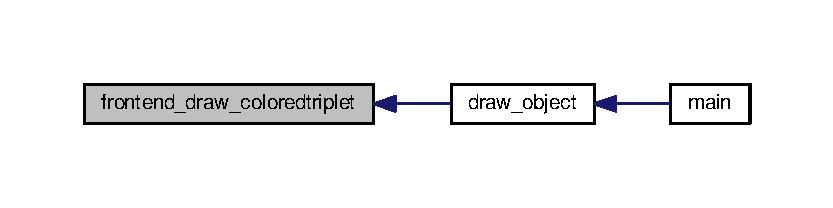
\includegraphics[width=350pt]{frontend__opengl__linux_8c_a0443993e9b09570d3b9ab2a6353be8c0_icgraph}
\end{center}
\end{figure}


\hypertarget{frontend__opengl__linux_8c_a532cd8517ad651db90c6e979addebf82}{\index{frontend\-\_\-opengl\-\_\-linux.\-c@{frontend\-\_\-opengl\-\_\-linux.\-c}!frontend\-\_\-draw\-\_\-point@{frontend\-\_\-draw\-\_\-point}}
\index{frontend\-\_\-draw\-\_\-point@{frontend\-\_\-draw\-\_\-point}!frontend_opengl_linux.c@{frontend\-\_\-opengl\-\_\-linux.\-c}}
\subsubsection[{frontend\-\_\-draw\-\_\-point}]{\setlength{\rightskip}{0pt plus 5cm}void frontend\-\_\-draw\-\_\-point (
\begin{DoxyParamCaption}
\item[{struct {\bf ipoint\-\_\-t} $\ast$}]{point, }
\item[{struct {\bf icolor\-\_\-t}}]{color}
\end{DoxyParamCaption}
)}}\label{frontend__opengl__linux_8c_a532cd8517ad651db90c6e979addebf82}


Definition at line 141 of file frontend\-\_\-opengl\-\_\-linux.\-c.


\begin{DoxyCode}
142 \{
143         glBegin(GL\_POINTS);
144                 glColor3f((\textcolor{keywordtype}{float})color.\hyperlink{structicolor__t_af41be99aa200064979c76e29d00d4aff}{r}, (\textcolor{keywordtype}{float})color.\hyperlink{structicolor__t_a3cf0a9335bbc32fc211d22f3ef502110}{g}, (\textcolor{keywordtype}{float})color.\hyperlink{structicolor__t_acb75f6cdb4866b33921bde0c5f9000ce}{b});
145                 glVertex3f(point->\hyperlink{structipoint__t_a345608e139b0709cc281139e3ed6328d}{x}, point->\hyperlink{structipoint__t_a88ca543f1508de060b4738cfebb51b04}{y}, (\textcolor{keywordtype}{float}) point->\hyperlink{structipoint__t_ad1680bc07190dabf544e86824b82e44b}{z});
146         glEnd();
147 \}
\end{DoxyCode}
\hypertarget{frontend__opengl__linux_8c_a3e3ddec01ee228bbd7e9bce1779e2f74}{\index{frontend\-\_\-opengl\-\_\-linux.\-c@{frontend\-\_\-opengl\-\_\-linux.\-c}!frontend\-\_\-draw\-\_\-rectangle@{frontend\-\_\-draw\-\_\-rectangle}}
\index{frontend\-\_\-draw\-\_\-rectangle@{frontend\-\_\-draw\-\_\-rectangle}!frontend_opengl_linux.c@{frontend\-\_\-opengl\-\_\-linux.\-c}}
\subsubsection[{frontend\-\_\-draw\-\_\-rectangle}]{\setlength{\rightskip}{0pt plus 5cm}void frontend\-\_\-draw\-\_\-rectangle (
\begin{DoxyParamCaption}
\item[{struct {\bf ipoint\-\_\-t} $\ast$}]{p1, }
\item[{struct {\bf ipoint\-\_\-t} $\ast$}]{p2, }
\item[{struct {\bf icolor\-\_\-t}}]{color}
\end{DoxyParamCaption}
)}}\label{frontend__opengl__linux_8c_a3e3ddec01ee228bbd7e9bce1779e2f74}


Definition at line 129 of file frontend\-\_\-opengl\-\_\-linux.\-c.


\begin{DoxyCode}
130 \{
131         \textcolor{keywordtype}{float} z = (float) p1->\hyperlink{structipoint__t_ad1680bc07190dabf544e86824b82e44b}{z};
132         glBegin(GL\_QUADS);
133                 glColor3f(color.\hyperlink{structicolor__t_af41be99aa200064979c76e29d00d4aff}{r}, color.\hyperlink{structicolor__t_a3cf0a9335bbc32fc211d22f3ef502110}{g}, color.\hyperlink{structicolor__t_acb75f6cdb4866b33921bde0c5f9000ce}{b});
134                 glVertex3f(p1->\hyperlink{structipoint__t_a345608e139b0709cc281139e3ed6328d}{x}, p1->\hyperlink{structipoint__t_a88ca543f1508de060b4738cfebb51b04}{y}, z);
135                 glVertex3f(p2->\hyperlink{structipoint__t_a345608e139b0709cc281139e3ed6328d}{x}, p1->\hyperlink{structipoint__t_a88ca543f1508de060b4738cfebb51b04}{y}, z);
136                 glVertex3f(p2->\hyperlink{structipoint__t_a345608e139b0709cc281139e3ed6328d}{x}, p2->\hyperlink{structipoint__t_a88ca543f1508de060b4738cfebb51b04}{y}, z);
137                 glVertex3f(p1->\hyperlink{structipoint__t_a345608e139b0709cc281139e3ed6328d}{x}, p2->\hyperlink{structipoint__t_a88ca543f1508de060b4738cfebb51b04}{y}, z);
138         glEnd();
139 \}
\end{DoxyCode}
\hypertarget{frontend__opengl__linux_8c_a5f1d2e26db40b3636fb218810a872a03}{\index{frontend\-\_\-opengl\-\_\-linux.\-c@{frontend\-\_\-opengl\-\_\-linux.\-c}!frontend\-\_\-free@{frontend\-\_\-free}}
\index{frontend\-\_\-free@{frontend\-\_\-free}!frontend_opengl_linux.c@{frontend\-\_\-opengl\-\_\-linux.\-c}}
\subsubsection[{frontend\-\_\-free}]{\setlength{\rightskip}{0pt plus 5cm}void frontend\-\_\-free (
\begin{DoxyParamCaption}
{}
\end{DoxyParamCaption}
)}}\label{frontend__opengl__linux_8c_a5f1d2e26db40b3636fb218810a872a03}


Definition at line 112 of file frontend\-\_\-opengl\-\_\-linux.\-c.


\begin{DoxyCode}
113 \{
114         printf(\textcolor{stringliteral}{"Freeing frontend resources...\(\backslash\)n"});
115         glXMakeCurrent(\hyperlink{frontend__opengl__linux_8h_a7d43b3edf58f8d85a89852ab95b740f6}{dpy}, None, NULL);
116         glXDestroyContext(\hyperlink{frontend__opengl__linux_8h_a7d43b3edf58f8d85a89852ab95b740f6}{dpy}, \hyperlink{frontend__opengl__linux_8h_a865db36501e45073170bee430ee35fc3}{glc});
117         XDestroyWindow(\hyperlink{frontend__opengl__linux_8h_a7d43b3edf58f8d85a89852ab95b740f6}{dpy}, \hyperlink{frontend__opengl__linux_8h_af5e9cbaf11bc8c0c330917f546d0045f}{win});
118         XCloseDisplay(\hyperlink{frontend__opengl__linux_8h_a7d43b3edf58f8d85a89852ab95b740f6}{dpy});
119 \}
\end{DoxyCode}


Here is the caller graph for this function\-:\nopagebreak
\begin{figure}[H]
\begin{center}
\leavevmode
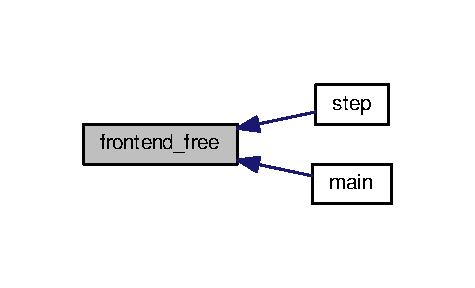
\includegraphics[width=228pt]{frontend__opengl__linux_8c_a5f1d2e26db40b3636fb218810a872a03_icgraph}
\end{center}
\end{figure}


\hypertarget{frontend__opengl__linux_8c_a4cb194a7e9456fffef751e2a311735eb}{\index{frontend\-\_\-opengl\-\_\-linux.\-c@{frontend\-\_\-opengl\-\_\-linux.\-c}!frontend\-\_\-initialize@{frontend\-\_\-initialize}}
\index{frontend\-\_\-initialize@{frontend\-\_\-initialize}!frontend_opengl_linux.c@{frontend\-\_\-opengl\-\_\-linux.\-c}}
\subsubsection[{frontend\-\_\-initialize}]{\setlength{\rightskip}{0pt plus 5cm}void frontend\-\_\-initialize (
\begin{DoxyParamCaption}
{}
\end{DoxyParamCaption}
)}}\label{frontend__opengl__linux_8c_a4cb194a7e9456fffef751e2a311735eb}


Definition at line 27 of file frontend\-\_\-opengl\-\_\-linux.\-c.


\begin{DoxyCode}
28 \{
29         \textcolor{comment}{//att = \{ GLX\_RGBA, GLX\_DEPTH\_SIZE, 24, GLX\_DOUBLEBUFFER, None \};}
30         \hyperlink{frontend__opengl__linux_8h_a5222c83ddcc16d2021dab765c97f6955}{att}[0] = GLX\_RGBA;
31         \hyperlink{frontend__opengl__linux_8h_a5222c83ddcc16d2021dab765c97f6955}{att}[1] = GLX\_DEPTH\_SIZE;
32         \hyperlink{frontend__opengl__linux_8h_a5222c83ddcc16d2021dab765c97f6955}{att}[2] = 24;
33         \hyperlink{frontend__opengl__linux_8h_a5222c83ddcc16d2021dab765c97f6955}{att}[3] = GLX\_DOUBLEBUFFER;
34         \hyperlink{frontend__opengl__linux_8h_a5222c83ddcc16d2021dab765c97f6955}{att}[4] = None;
35         \hyperlink{frontend__opengl__linux_8h_a7d43b3edf58f8d85a89852ab95b740f6}{dpy} = XOpenDisplay(NULL);
36         
37         \textcolor{keywordflow}{if}(\hyperlink{frontend__opengl__linux_8h_a7d43b3edf58f8d85a89852ab95b740f6}{dpy} == NULL) \{
38                 printf(\textcolor{stringliteral}{"\(\backslash\)n\(\backslash\)tcannot connect to X server\(\backslash\)n\(\backslash\)n"});
39                 exit(0);
40         \}
41 
42         \hyperlink{frontend__opengl__linux_8h_a67efd2aa4387dcb1b33df1f044512a16}{root} = DefaultRootWindow(\hyperlink{frontend__opengl__linux_8h_a7d43b3edf58f8d85a89852ab95b740f6}{dpy});
43 
44         \hyperlink{frontend__opengl__linux_8h_a6ea38ddc009c6f56a768347fa8cca7fc}{vi} = glXChooseVisual(\hyperlink{frontend__opengl__linux_8h_a7d43b3edf58f8d85a89852ab95b740f6}{dpy}, 0, \hyperlink{frontend__opengl__linux_8h_a5222c83ddcc16d2021dab765c97f6955}{att});
45 
46         \textcolor{keywordflow}{if}(\hyperlink{frontend__opengl__linux_8h_a6ea38ddc009c6f56a768347fa8cca7fc}{vi} == NULL) \{
47                 printf(\textcolor{stringliteral}{"\(\backslash\)n\(\backslash\)tno appropriate visual found\(\backslash\)n\(\backslash\)n"});
48                 exit(0);
49         \} 
50         \textcolor{keywordflow}{else} \{
51                 printf(\textcolor{stringliteral}{"\(\backslash\)n\(\backslash\)tvisual %p selected\(\backslash\)n"}, (\textcolor{keywordtype}{void} *)\hyperlink{frontend__opengl__linux_8h_a6ea38ddc009c6f56a768347fa8cca7fc}{vi}->visualid);
52         \}
53 
54         \hyperlink{frontend__opengl__linux_8h_ae9e16ee22daffbbbbf59f6c841c2ab75}{cmap} = XCreateColormap(\hyperlink{frontend__opengl__linux_8h_a7d43b3edf58f8d85a89852ab95b740f6}{dpy}, \hyperlink{frontend__opengl__linux_8h_a67efd2aa4387dcb1b33df1f044512a16}{root}, \hyperlink{frontend__opengl__linux_8h_a6ea38ddc009c6f56a768347fa8cca7fc}{vi}->visual, AllocNone);
55 
56         \hyperlink{frontend__opengl__linux_8h_a89fc0a57cdcd1daf998256dd0f62acd2}{swa}.colormap = \hyperlink{frontend__opengl__linux_8h_ae9e16ee22daffbbbbf59f6c841c2ab75}{cmap};
57         \hyperlink{frontend__opengl__linux_8h_a89fc0a57cdcd1daf998256dd0f62acd2}{swa}.event\_mask = ExposureMask | KeyPressMask;
58 
59         \hyperlink{frontend__opengl__linux_8h_af5e9cbaf11bc8c0c330917f546d0045f}{win} = XCreateWindow(\hyperlink{frontend__opengl__linux_8h_a7d43b3edf58f8d85a89852ab95b740f6}{dpy}, \hyperlink{frontend__opengl__linux_8h_a67efd2aa4387dcb1b33df1f044512a16}{root}, 0, 0, 600, 600, 0,
60                                 \hyperlink{frontend__opengl__linux_8h_a6ea38ddc009c6f56a768347fa8cca7fc}{vi}->depth, InputOutput, \hyperlink{frontend__opengl__linux_8h_a6ea38ddc009c6f56a768347fa8cca7fc}{vi}->visual,
61                                 CWColormap | CWEventMask, &\hyperlink{frontend__opengl__linux_8h_a89fc0a57cdcd1daf998256dd0f62acd2}{swa});
62 
63         XMapWindow(\hyperlink{frontend__opengl__linux_8h_a7d43b3edf58f8d85a89852ab95b740f6}{dpy}, \hyperlink{frontend__opengl__linux_8h_af5e9cbaf11bc8c0c330917f546d0045f}{win});
64 
65         XStoreName(\hyperlink{frontend__opengl__linux_8h_a7d43b3edf58f8d85a89852ab95b740f6}{dpy}, \hyperlink{frontend__opengl__linux_8h_af5e9cbaf11bc8c0c330917f546d0045f}{win}, \textcolor{stringliteral}{"VERY SIMPLE APPLICATION"});
66 
67         \hyperlink{frontend__opengl__linux_8h_a865db36501e45073170bee430ee35fc3}{glc} = glXCreateContext(\hyperlink{frontend__opengl__linux_8h_a7d43b3edf58f8d85a89852ab95b740f6}{dpy}, \hyperlink{frontend__opengl__linux_8h_a6ea38ddc009c6f56a768347fa8cca7fc}{vi}, NULL, GL\_TRUE);
68         glXMakeCurrent(\hyperlink{frontend__opengl__linux_8h_a7d43b3edf58f8d85a89852ab95b740f6}{dpy}, \hyperlink{frontend__opengl__linux_8h_af5e9cbaf11bc8c0c330917f546d0045f}{win}, \hyperlink{frontend__opengl__linux_8h_a865db36501e45073170bee430ee35fc3}{glc});
69 
70         glDisable(GL\_DEPTH\_TEST);
71 \}
\end{DoxyCode}


Here is the caller graph for this function\-:\nopagebreak
\begin{figure}[H]
\begin{center}
\leavevmode
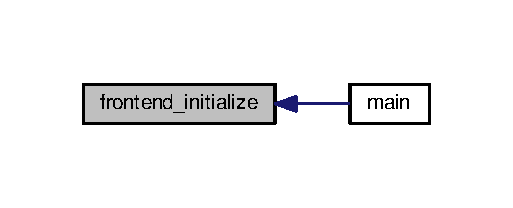
\includegraphics[width=246pt]{frontend__opengl__linux_8c_a4cb194a7e9456fffef751e2a311735eb_icgraph}
\end{center}
\end{figure}


\hypertarget{frontend__opengl__linux_8c_aeac975aee6becbb83f7fac162d290fe0}{\index{frontend\-\_\-opengl\-\_\-linux.\-c@{frontend\-\_\-opengl\-\_\-linux.\-c}!frontend\-\_\-initialize\-\_\-viewspace@{frontend\-\_\-initialize\-\_\-viewspace}}
\index{frontend\-\_\-initialize\-\_\-viewspace@{frontend\-\_\-initialize\-\_\-viewspace}!frontend_opengl_linux.c@{frontend\-\_\-opengl\-\_\-linux.\-c}}
\subsubsection[{frontend\-\_\-initialize\-\_\-viewspace}]{\setlength{\rightskip}{0pt plus 5cm}void frontend\-\_\-initialize\-\_\-viewspace (
\begin{DoxyParamCaption}
\item[{float}]{x1, }
\item[{float}]{x2, }
\item[{float}]{y1, }
\item[{float}]{y2, }
\item[{int}]{num\-\_\-z\-\_\-levels, }
\item[{struct {\bf ifrontendstate\-\_\-t} $\ast$}]{state}
\end{DoxyParamCaption}
)}}\label{frontend__opengl__linux_8c_aeac975aee6becbb83f7fac162d290fe0}
\begin{DoxyReturn}{Returns}
a bitmap with the 0 byte being the number of \char`\"{}near\char`\"{} z-\/levels and the 1 byte being the number of \char`\"{}far\char`\"{} z-\/levels 
\end{DoxyReturn}


Definition at line 76 of file frontend\-\_\-opengl\-\_\-linux.\-c.


\begin{DoxyCode}
77 \{
78         state->\hyperlink{structifrontendstate__t_afb7c49000e593f77bcb30b1ae4384ded}{background\_color} = malloc(\textcolor{keyword}{sizeof}(\textcolor{keyword}{struct} \hyperlink{structicolor__t}{icolor\_t}));
79         state->\hyperlink{structifrontendstate__t_ac81d750ec8cd1ba1d44e2c0f55bea687}{drawing\_color} = malloc(\textcolor{keyword}{sizeof}(\textcolor{keyword}{struct} \hyperlink{structicolor__t}{icolor\_t}));
80         state->\hyperlink{structifrontendstate__t_a54ee910059c66c18fa1bb1555d0e61c5}{left} = x1;
81         state->\hyperlink{structifrontendstate__t_a7c304035e472522fb01b3bb85b37eef8}{right} = x2;
82         state->\hyperlink{structifrontendstate__t_adc025993349dceae53dfe235f84fdef2}{bottom} = y1;
83         state->\hyperlink{structifrontendstate__t_afda9cb91a47174c6e95a4888918964f4}{top} = y2;
84         state->\hyperlink{structifrontendstate__t_aefb96a4cd8758bcd9a3e5b506290adca}{z\_levels} = num\_z\_levels;
85         state->\hyperlink{structifrontendstate__t_ad30593dd0b69372008108075c55cfe27}{num\_regions} = 0;
86         state->\hyperlink{structifrontendstate__t_a42ce77321ecea4fde68dd68b7f0f2283}{regions} = NULL;
87         \hyperlink{icoordinates_8c_a4507e51c1f2470e19e8ff5a77adf54bd}{icreate\_region}(0, 0, 100, 100, state);
88         \textcolor{keywordtype}{int} i;
89         \textcolor{keywordflow}{for} (i = 0; i < 256; i++) \{
90                 state->\hyperlink{structifrontendstate__t_a5bb9423c4ba5f86cd8a0d50575031952}{onkeyup\_handlers}[i]   = \hyperlink{frontend_8c_af20744b431ee1afa0043f15e5e2f9207}{inew\_eventhandler}(NULL, 
      NULL, i);
91                 state->\hyperlink{structifrontendstate__t_ad8fd468eaec37b949af562b39ad20d5a}{onkeydown\_handlers}[i] = 
      \hyperlink{frontend_8c_af20744b431ee1afa0043f15e5e2f9207}{inew\_eventhandler}(NULL, NULL, i);
92         \}
93 \}
\end{DoxyCode}


Here is the call graph for this function\-:\nopagebreak
\begin{figure}[H]
\begin{center}
\leavevmode
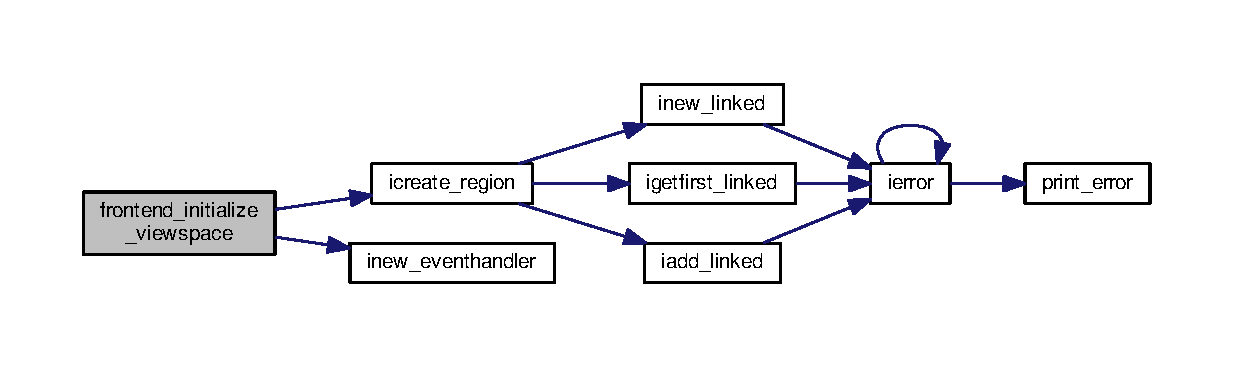
\includegraphics[width=350pt]{frontend__opengl__linux_8c_aeac975aee6becbb83f7fac162d290fe0_cgraph}
\end{center}
\end{figure}




Here is the caller graph for this function\-:\nopagebreak
\begin{figure}[H]
\begin{center}
\leavevmode
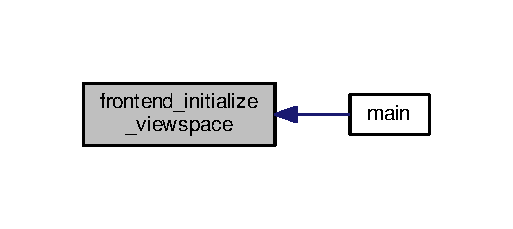
\includegraphics[width=246pt]{frontend__opengl__linux_8c_aeac975aee6becbb83f7fac162d290fe0_icgraph}
\end{center}
\end{figure}


\hypertarget{frontend__opengl__linux_8c_ad8a729cc49f33a0037227c75e1979ada}{\index{frontend\-\_\-opengl\-\_\-linux.\-c@{frontend\-\_\-opengl\-\_\-linux.\-c}!frontend\-\_\-reset\-\_\-viewspace@{frontend\-\_\-reset\-\_\-viewspace}}
\index{frontend\-\_\-reset\-\_\-viewspace@{frontend\-\_\-reset\-\_\-viewspace}!frontend_opengl_linux.c@{frontend\-\_\-opengl\-\_\-linux.\-c}}
\subsubsection[{frontend\-\_\-reset\-\_\-viewspace}]{\setlength{\rightskip}{0pt plus 5cm}void frontend\-\_\-reset\-\_\-viewspace (
\begin{DoxyParamCaption}
\item[{struct {\bf ifrontendstate\-\_\-t} $\ast$}]{state}
\end{DoxyParamCaption}
)}}\label{frontend__opengl__linux_8c_ad8a729cc49f33a0037227c75e1979ada}


Definition at line 95 of file frontend\-\_\-opengl\-\_\-linux.\-c.


\begin{DoxyCode}
96 \{
97         glClearColor((\textcolor{keywordtype}{float})\hyperlink{iprimitives_8c_afc34677b05531522408374dc02a31f40}{red}(*state->\hyperlink{structifrontendstate__t_afb7c49000e593f77bcb30b1ae4384ded}{background\_color})/256.,
98                      (\textcolor{keywordtype}{float})\hyperlink{iprimitives_8c_abc6932dd227752af4dbf7fac0b6e3291}{green}(*state->\hyperlink{structifrontendstate__t_afb7c49000e593f77bcb30b1ae4384ded}{background\_color})/256.,
99                      (\textcolor{keywordtype}{float})\hyperlink{iprimitives_8c_a03066bd036a134534caeec08526b7269}{blue}(*state->\hyperlink{structifrontendstate__t_afb7c49000e593f77bcb30b1ae4384ded}{background\_color})/256., 1.0);
100         glClear(GL\_COLOR\_BUFFER\_BIT | GL\_DEPTH\_BUFFER\_BIT);
101 
102         glMatrixMode(GL\_PROJECTION);
103         glLoadIdentity();
104         glOrtho(state->\hyperlink{structifrontendstate__t_a54ee910059c66c18fa1bb1555d0e61c5}{left}, state->\hyperlink{structifrontendstate__t_a7c304035e472522fb01b3bb85b37eef8}{right}, state->\hyperlink{structifrontendstate__t_adc025993349dceae53dfe235f84fdef2}{bottom}, state->
      \hyperlink{structifrontendstate__t_afda9cb91a47174c6e95a4888918964f4}{top}, state->\hyperlink{structifrontendstate__t_aefb96a4cd8758bcd9a3e5b506290adca}{z\_levels}, 0);
105 
106         glMatrixMode(GL\_MODELVIEW);
107         glLoadIdentity();
108         gluLookAt(0., 0., 10., 0., 0., 0., 0., 1., 0.);
109 \}
\end{DoxyCode}


Here is the call graph for this function\-:\nopagebreak
\begin{figure}[H]
\begin{center}
\leavevmode
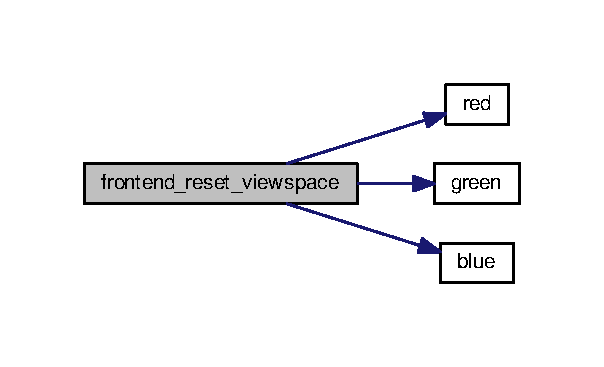
\includegraphics[width=290pt]{frontend__opengl__linux_8c_ad8a729cc49f33a0037227c75e1979ada_cgraph}
\end{center}
\end{figure}




Here is the caller graph for this function\-:\nopagebreak
\begin{figure}[H]
\begin{center}
\leavevmode
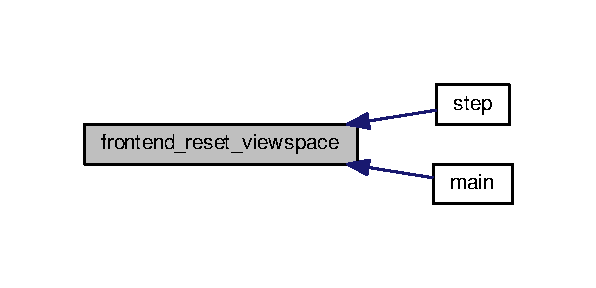
\includegraphics[width=286pt]{frontend__opengl__linux_8c_ad8a729cc49f33a0037227c75e1979ada_icgraph}
\end{center}
\end{figure}


\hypertarget{frontend__opengl__linux_8c_a740fe64ba30a741771700f190e164a9c}{\index{frontend\-\_\-opengl\-\_\-linux.\-c@{frontend\-\_\-opengl\-\_\-linux.\-c}!frontend\-\_\-update@{frontend\-\_\-update}}
\index{frontend\-\_\-update@{frontend\-\_\-update}!frontend_opengl_linux.c@{frontend\-\_\-opengl\-\_\-linux.\-c}}
\subsubsection[{frontend\-\_\-update}]{\setlength{\rightskip}{0pt plus 5cm}void frontend\-\_\-update (
\begin{DoxyParamCaption}
\item[{struct {\bf ifrontendstate\-\_\-t} $\ast$}]{state}
\end{DoxyParamCaption}
)}}\label{frontend__opengl__linux_8c_a740fe64ba30a741771700f190e164a9c}


Definition at line 121 of file frontend\-\_\-opengl\-\_\-linux.\-c.


\begin{DoxyCode}
122 \{
123         XGetWindowAttributes(\hyperlink{frontend__opengl__linux_8h_a7d43b3edf58f8d85a89852ab95b740f6}{dpy}, \hyperlink{frontend__opengl__linux_8h_af5e9cbaf11bc8c0c330917f546d0045f}{win}, &\hyperlink{frontend__opengl__linux_8h_aba75c5c2ba56afc9f1960cb36460d247}{gwa});
124         glViewport(0, 0, \hyperlink{frontend__opengl__linux_8h_aba75c5c2ba56afc9f1960cb36460d247}{gwa}.width, \hyperlink{frontend__opengl__linux_8h_aba75c5c2ba56afc9f1960cb36460d247}{gwa}.height);
125         \textcolor{comment}{//DrawAQuad(); }
126         glXSwapBuffers(\hyperlink{frontend__opengl__linux_8h_a7d43b3edf58f8d85a89852ab95b740f6}{dpy}, \hyperlink{frontend__opengl__linux_8h_af5e9cbaf11bc8c0c330917f546d0045f}{win});
127 \}
\end{DoxyCode}


Here is the caller graph for this function\-:\nopagebreak
\begin{figure}[H]
\begin{center}
\leavevmode
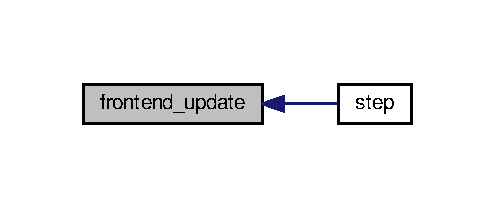
\includegraphics[width=238pt]{frontend__opengl__linux_8c_a740fe64ba30a741771700f190e164a9c_icgraph}
\end{center}
\end{figure}


\hypertarget{frontend__opengl__linux_8c_a606f78ac8a9bdf59c7a520da2b2052e0}{\index{frontend\-\_\-opengl\-\_\-linux.\-c@{frontend\-\_\-opengl\-\_\-linux.\-c}!step@{step}}
\index{step@{step}!frontend_opengl_linux.c@{frontend\-\_\-opengl\-\_\-linux.\-c}}
\subsubsection[{step}]{\setlength{\rightskip}{0pt plus 5cm}int step (
\begin{DoxyParamCaption}
\item[{struct {\bf ifrontendstate\-\_\-t} $\ast$}]{state}
\end{DoxyParamCaption}
)}}\label{frontend__opengl__linux_8c_a606f78ac8a9bdf59c7a520da2b2052e0}


Definition at line 170 of file frontend\-\_\-opengl\-\_\-linux.\-c.


\begin{DoxyCode}
171 \{
172         XNextEvent(\hyperlink{frontend__opengl__linux_8h_a7d43b3edf58f8d85a89852ab95b740f6}{dpy}, &\hyperlink{frontend__opengl__linux_8h_aa8a168b034976fcc1a0896de4a6ea64d}{xev});
173         \textcolor{keywordflow}{if} (\hyperlink{frontend__opengl__linux_8h_aa8a168b034976fcc1a0896de4a6ea64d}{xev}.type == Expose)
174                 \hyperlink{frontend__opengl__linux_8c_a740fe64ba30a741771700f190e164a9c}{frontend\_update}(state);
175         \textcolor{keywordflow}{else} \textcolor{keywordflow}{if}(\hyperlink{frontend__opengl__linux_8h_aa8a168b034976fcc1a0896de4a6ea64d}{xev}.type == KeyPress) \{
176                 \textcolor{keyword}{struct }\hyperlink{structievent__handler}{ievent\_handler} *h = state->
      \hyperlink{structifrontendstate__t_ad8fd468eaec37b949af562b39ad20d5a}{onkeydown\_handlers}[\hyperlink{frontend__opengl__linux_8h_aa8a168b034976fcc1a0896de4a6ea64d}{xev}.xkey.keycode];
177                 *(h->\hyperlink{structievent__handler_a320eaffc01d119279ead9c5ad877c6da}{handler})(h->\hyperlink{structievent__handler_ac6b4e6b5b95ada7b0d9985f738ffe1e5}{args}, (\textcolor{keywordtype}{void}*)&(\hyperlink{frontend__opengl__linux_8h_aa8a168b034976fcc1a0896de4a6ea64d}{xev}.xkey));
178         \}
179         \textcolor{keywordflow}{else} \textcolor{keywordflow}{if} (\hyperlink{frontend__opengl__linux_8h_aa8a168b034976fcc1a0896de4a6ea64d}{xev}.type == KeyRelease) \{ 
180                 \textcolor{keyword}{struct }\hyperlink{structievent__handler}{ievent\_handler} *h = state->\hyperlink{structifrontendstate__t_a5bb9423c4ba5f86cd8a0d50575031952}{onkeyup\_handlers}[
      \hyperlink{frontend__opengl__linux_8h_aa8a168b034976fcc1a0896de4a6ea64d}{xev}.xkey.keycode];
181                 *(h->\hyperlink{structievent__handler_a320eaffc01d119279ead9c5ad877c6da}{handler})(h->\hyperlink{structievent__handler_ac6b4e6b5b95ada7b0d9985f738ffe1e5}{args}, (\textcolor{keywordtype}{void}*)&(\hyperlink{frontend__opengl__linux_8h_aa8a168b034976fcc1a0896de4a6ea64d}{xev}.xkey));
182         \}
183         \textcolor{keywordflow}{else} \textcolor{keywordflow}{if} (\hyperlink{frontend__opengl__linux_8h_aa8a168b034976fcc1a0896de4a6ea64d}{xev}.type == ClientMessage) \{
184                 \hyperlink{frontend__opengl__linux_8c_a5f1d2e26db40b3636fb218810a872a03}{frontend\_free}();
185                 \textcolor{keywordflow}{return} 1;
186         \}
187         \hyperlink{frontend__opengl__linux_8c_a740fe64ba30a741771700f190e164a9c}{frontend\_update}(state);
188         \hyperlink{frontend__opengl__linux_8c_ad8a729cc49f33a0037227c75e1979ada}{frontend\_reset\_viewspace}(state);
189         \textcolor{keywordflow}{return} 0;
190 \}
\end{DoxyCode}


Here is the call graph for this function\-:\nopagebreak
\begin{figure}[H]
\begin{center}
\leavevmode
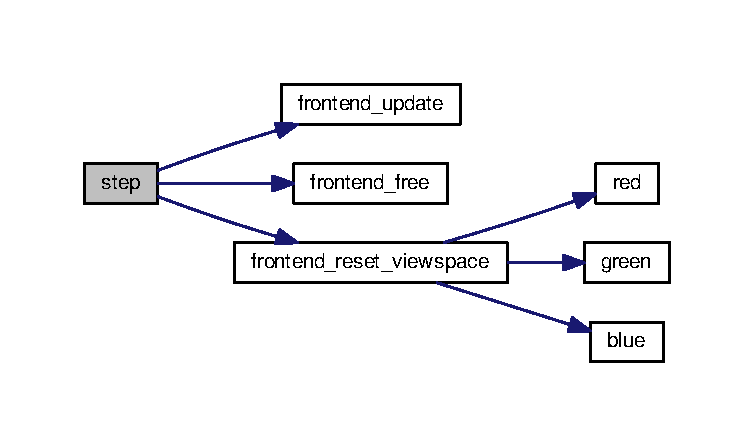
\includegraphics[width=350pt]{frontend__opengl__linux_8c_a606f78ac8a9bdf59c7a520da2b2052e0_cgraph}
\end{center}
\end{figure}



\hypertarget{frontend__opengl__linux_8h}{\section{src/frontends/frontend\-\_\-opengl\-\_\-linux.h File Reference}
\label{frontend__opengl__linux_8h}\index{src/frontends/frontend\-\_\-opengl\-\_\-linux.\-h@{src/frontends/frontend\-\_\-opengl\-\_\-linux.\-h}}
}
{\ttfamily \#include $<$X11/\-X.\-h$>$}\\*
{\ttfamily \#include $<$X11/\-Xlib.\-h$>$}\\*
{\ttfamily \#include $<$G\-L/gl.\-h$>$}\\*
{\ttfamily \#include $<$G\-L/glx.\-h$>$}\\*
{\ttfamily \#include $<$G\-L/glu.\-h$>$}\\*
{\ttfamily \#include \char`\"{}frontend.\-h\char`\"{}}\\*
{\ttfamily \#include \char`\"{}../icoordinates.\-h\char`\"{}}\\*
Include dependency graph for frontend\-\_\-opengl\-\_\-linux.\-h\-:\nopagebreak
\begin{figure}[H]
\begin{center}
\leavevmode
\includegraphics[width=350pt]{frontend__opengl__linux_8h__incl}
\end{center}
\end{figure}
This graph shows which files directly or indirectly include this file\-:
\nopagebreak
\begin{figure}[H]
\begin{center}
\leavevmode
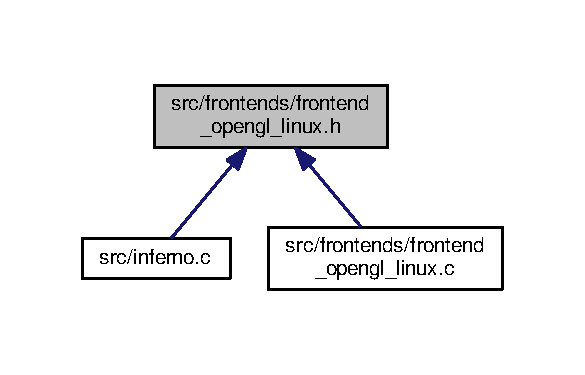
\includegraphics[width=281pt]{frontend__opengl__linux_8h__dep__incl}
\end{center}
\end{figure}
\subsection*{Functions}
\begin{DoxyCompactItemize}
\item 
void \hyperlink{frontend__opengl__linux_8h_a345706a31501f213b1c7ad1825d4628f}{Draw\-A\-Quad} ()
\end{DoxyCompactItemize}
\subsection*{Variables}
\begin{DoxyCompactItemize}
\item 
Display $\ast$ \hyperlink{frontend__opengl__linux_8h_a7d43b3edf58f8d85a89852ab95b740f6}{dpy}
\item 
Window \hyperlink{frontend__opengl__linux_8h_a67efd2aa4387dcb1b33df1f044512a16}{root}
\item 
G\-Lint \hyperlink{frontend__opengl__linux_8h_a5222c83ddcc16d2021dab765c97f6955}{att} \mbox{[}5\mbox{]}
\item 
X\-Visual\-Info $\ast$ \hyperlink{frontend__opengl__linux_8h_a6ea38ddc009c6f56a768347fa8cca7fc}{vi}
\item 
Colormap \hyperlink{frontend__opengl__linux_8h_ae9e16ee22daffbbbbf59f6c841c2ab75}{cmap}
\item 
X\-Set\-Window\-Attributes \hyperlink{frontend__opengl__linux_8h_a89fc0a57cdcd1daf998256dd0f62acd2}{swa}
\item 
Window \hyperlink{frontend__opengl__linux_8h_af5e9cbaf11bc8c0c330917f546d0045f}{win}
\item 
G\-L\-X\-Context \hyperlink{frontend__opengl__linux_8h_a865db36501e45073170bee430ee35fc3}{glc}
\item 
X\-Window\-Attributes \hyperlink{frontend__opengl__linux_8h_aba75c5c2ba56afc9f1960cb36460d247}{gwa}
\item 
X\-Event \hyperlink{frontend__opengl__linux_8h_aa8a168b034976fcc1a0896de4a6ea64d}{xev}
\end{DoxyCompactItemize}


\subsection{Function Documentation}
\hypertarget{frontend__opengl__linux_8h_a345706a31501f213b1c7ad1825d4628f}{\index{frontend\-\_\-opengl\-\_\-linux.\-h@{frontend\-\_\-opengl\-\_\-linux.\-h}!Draw\-A\-Quad@{Draw\-A\-Quad}}
\index{Draw\-A\-Quad@{Draw\-A\-Quad}!frontend_opengl_linux.h@{frontend\-\_\-opengl\-\_\-linux.\-h}}
\subsubsection[{Draw\-A\-Quad}]{\setlength{\rightskip}{0pt plus 5cm}void Draw\-A\-Quad (
\begin{DoxyParamCaption}
{}
\end{DoxyParamCaption}
)}}\label{frontend__opengl__linux_8h_a345706a31501f213b1c7ad1825d4628f}


Definition at line 16 of file frontend\-\_\-opengl\-\_\-linux.\-c.


\begin{DoxyCode}
16                  \{
17         glBegin(GL\_QUADS);
18         \textcolor{comment}{/*glColor3f(1., 0., 0.); glVertex3f(-.75, -.75, 0.);}
19 \textcolor{comment}{        glColor3f(0., 1., 0.); glVertex3f( 75, -.75, 0.);}
20 \textcolor{comment}{        glColor3f(0., 0., 1.); glVertex3f( .75,  .75, 0.);}
21 \textcolor{comment}{        glColor3f(1., 1., 0.); glVertex3f(-.75,  .75, 0.);*/}
22         glColor3f(0., 0., 0.);
23         glVertex2f(0.0, 0.); glVertex2f(1., 0.); glVertex2f(1., 1.); glVertex2f(0., 1.);
24         glEnd();
25 \} 
\end{DoxyCode}


\subsection{Variable Documentation}
\hypertarget{frontend__opengl__linux_8h_a5222c83ddcc16d2021dab765c97f6955}{\index{frontend\-\_\-opengl\-\_\-linux.\-h@{frontend\-\_\-opengl\-\_\-linux.\-h}!att@{att}}
\index{att@{att}!frontend_opengl_linux.h@{frontend\-\_\-opengl\-\_\-linux.\-h}}
\subsubsection[{att}]{\setlength{\rightskip}{0pt plus 5cm}G\-Lint att\mbox{[}5\mbox{]}}}\label{frontend__opengl__linux_8h_a5222c83ddcc16d2021dab765c97f6955}


Definition at line 15 of file frontend\-\_\-opengl\-\_\-linux.\-h.

\hypertarget{frontend__opengl__linux_8h_ae9e16ee22daffbbbbf59f6c841c2ab75}{\index{frontend\-\_\-opengl\-\_\-linux.\-h@{frontend\-\_\-opengl\-\_\-linux.\-h}!cmap@{cmap}}
\index{cmap@{cmap}!frontend_opengl_linux.h@{frontend\-\_\-opengl\-\_\-linux.\-h}}
\subsubsection[{cmap}]{\setlength{\rightskip}{0pt plus 5cm}Colormap cmap}}\label{frontend__opengl__linux_8h_ae9e16ee22daffbbbbf59f6c841c2ab75}


Definition at line 17 of file frontend\-\_\-opengl\-\_\-linux.\-h.

\hypertarget{frontend__opengl__linux_8h_a7d43b3edf58f8d85a89852ab95b740f6}{\index{frontend\-\_\-opengl\-\_\-linux.\-h@{frontend\-\_\-opengl\-\_\-linux.\-h}!dpy@{dpy}}
\index{dpy@{dpy}!frontend_opengl_linux.h@{frontend\-\_\-opengl\-\_\-linux.\-h}}
\subsubsection[{dpy}]{\setlength{\rightskip}{0pt plus 5cm}Display$\ast$ dpy}}\label{frontend__opengl__linux_8h_a7d43b3edf58f8d85a89852ab95b740f6}


Definition at line 13 of file frontend\-\_\-opengl\-\_\-linux.\-h.

\hypertarget{frontend__opengl__linux_8h_a865db36501e45073170bee430ee35fc3}{\index{frontend\-\_\-opengl\-\_\-linux.\-h@{frontend\-\_\-opengl\-\_\-linux.\-h}!glc@{glc}}
\index{glc@{glc}!frontend_opengl_linux.h@{frontend\-\_\-opengl\-\_\-linux.\-h}}
\subsubsection[{glc}]{\setlength{\rightskip}{0pt plus 5cm}G\-L\-X\-Context glc}}\label{frontend__opengl__linux_8h_a865db36501e45073170bee430ee35fc3}


Definition at line 20 of file frontend\-\_\-opengl\-\_\-linux.\-h.

\hypertarget{frontend__opengl__linux_8h_aba75c5c2ba56afc9f1960cb36460d247}{\index{frontend\-\_\-opengl\-\_\-linux.\-h@{frontend\-\_\-opengl\-\_\-linux.\-h}!gwa@{gwa}}
\index{gwa@{gwa}!frontend_opengl_linux.h@{frontend\-\_\-opengl\-\_\-linux.\-h}}
\subsubsection[{gwa}]{\setlength{\rightskip}{0pt plus 5cm}X\-Window\-Attributes gwa}}\label{frontend__opengl__linux_8h_aba75c5c2ba56afc9f1960cb36460d247}


Definition at line 21 of file frontend\-\_\-opengl\-\_\-linux.\-h.

\hypertarget{frontend__opengl__linux_8h_a67efd2aa4387dcb1b33df1f044512a16}{\index{frontend\-\_\-opengl\-\_\-linux.\-h@{frontend\-\_\-opengl\-\_\-linux.\-h}!root@{root}}
\index{root@{root}!frontend_opengl_linux.h@{frontend\-\_\-opengl\-\_\-linux.\-h}}
\subsubsection[{root}]{\setlength{\rightskip}{0pt plus 5cm}Window root}}\label{frontend__opengl__linux_8h_a67efd2aa4387dcb1b33df1f044512a16}


Definition at line 14 of file frontend\-\_\-opengl\-\_\-linux.\-h.

\hypertarget{frontend__opengl__linux_8h_a89fc0a57cdcd1daf998256dd0f62acd2}{\index{frontend\-\_\-opengl\-\_\-linux.\-h@{frontend\-\_\-opengl\-\_\-linux.\-h}!swa@{swa}}
\index{swa@{swa}!frontend_opengl_linux.h@{frontend\-\_\-opengl\-\_\-linux.\-h}}
\subsubsection[{swa}]{\setlength{\rightskip}{0pt plus 5cm}X\-Set\-Window\-Attributes swa}}\label{frontend__opengl__linux_8h_a89fc0a57cdcd1daf998256dd0f62acd2}


Definition at line 18 of file frontend\-\_\-opengl\-\_\-linux.\-h.

\hypertarget{frontend__opengl__linux_8h_a6ea38ddc009c6f56a768347fa8cca7fc}{\index{frontend\-\_\-opengl\-\_\-linux.\-h@{frontend\-\_\-opengl\-\_\-linux.\-h}!vi@{vi}}
\index{vi@{vi}!frontend_opengl_linux.h@{frontend\-\_\-opengl\-\_\-linux.\-h}}
\subsubsection[{vi}]{\setlength{\rightskip}{0pt plus 5cm}X\-Visual\-Info$\ast$ vi}}\label{frontend__opengl__linux_8h_a6ea38ddc009c6f56a768347fa8cca7fc}


Definition at line 16 of file frontend\-\_\-opengl\-\_\-linux.\-h.

\hypertarget{frontend__opengl__linux_8h_af5e9cbaf11bc8c0c330917f546d0045f}{\index{frontend\-\_\-opengl\-\_\-linux.\-h@{frontend\-\_\-opengl\-\_\-linux.\-h}!win@{win}}
\index{win@{win}!frontend_opengl_linux.h@{frontend\-\_\-opengl\-\_\-linux.\-h}}
\subsubsection[{win}]{\setlength{\rightskip}{0pt plus 5cm}Window win}}\label{frontend__opengl__linux_8h_af5e9cbaf11bc8c0c330917f546d0045f}


Definition at line 19 of file frontend\-\_\-opengl\-\_\-linux.\-h.

\hypertarget{frontend__opengl__linux_8h_aa8a168b034976fcc1a0896de4a6ea64d}{\index{frontend\-\_\-opengl\-\_\-linux.\-h@{frontend\-\_\-opengl\-\_\-linux.\-h}!xev@{xev}}
\index{xev@{xev}!frontend_opengl_linux.h@{frontend\-\_\-opengl\-\_\-linux.\-h}}
\subsubsection[{xev}]{\setlength{\rightskip}{0pt plus 5cm}X\-Event xev}}\label{frontend__opengl__linux_8h_aa8a168b034976fcc1a0896de4a6ea64d}


Definition at line 22 of file frontend\-\_\-opengl\-\_\-linux.\-h.


\hypertarget{icoordinates_8c}{\section{src/icoordinates.c File Reference}
\label{icoordinates_8c}\index{src/icoordinates.\-c@{src/icoordinates.\-c}}
}
{\ttfamily \#include \char`\"{}frontend.\-h\char`\"{}}\\*
{\ttfamily \#include \char`\"{}icoordinates.\-h\char`\"{}}\\*
{\ttfamily \#include \char`\"{}error.\-h\char`\"{}}\\*
{\ttfamily \#include \char`\"{}iutils.\-h\char`\"{}}\\*
{\ttfamily \#include \char`\"{}itypes.\-h\char`\"{}}\\*
{\ttfamily \#include \char`\"{}iprettyconsole.\-h\char`\"{}}\\*
{\ttfamily \#include $<$stdlib.\-h$>$}\\*
{\ttfamily \#include $<$stdio.\-h$>$}\\*
Include dependency graph for icoordinates.\-c\-:\nopagebreak
\begin{figure}[H]
\begin{center}
\leavevmode
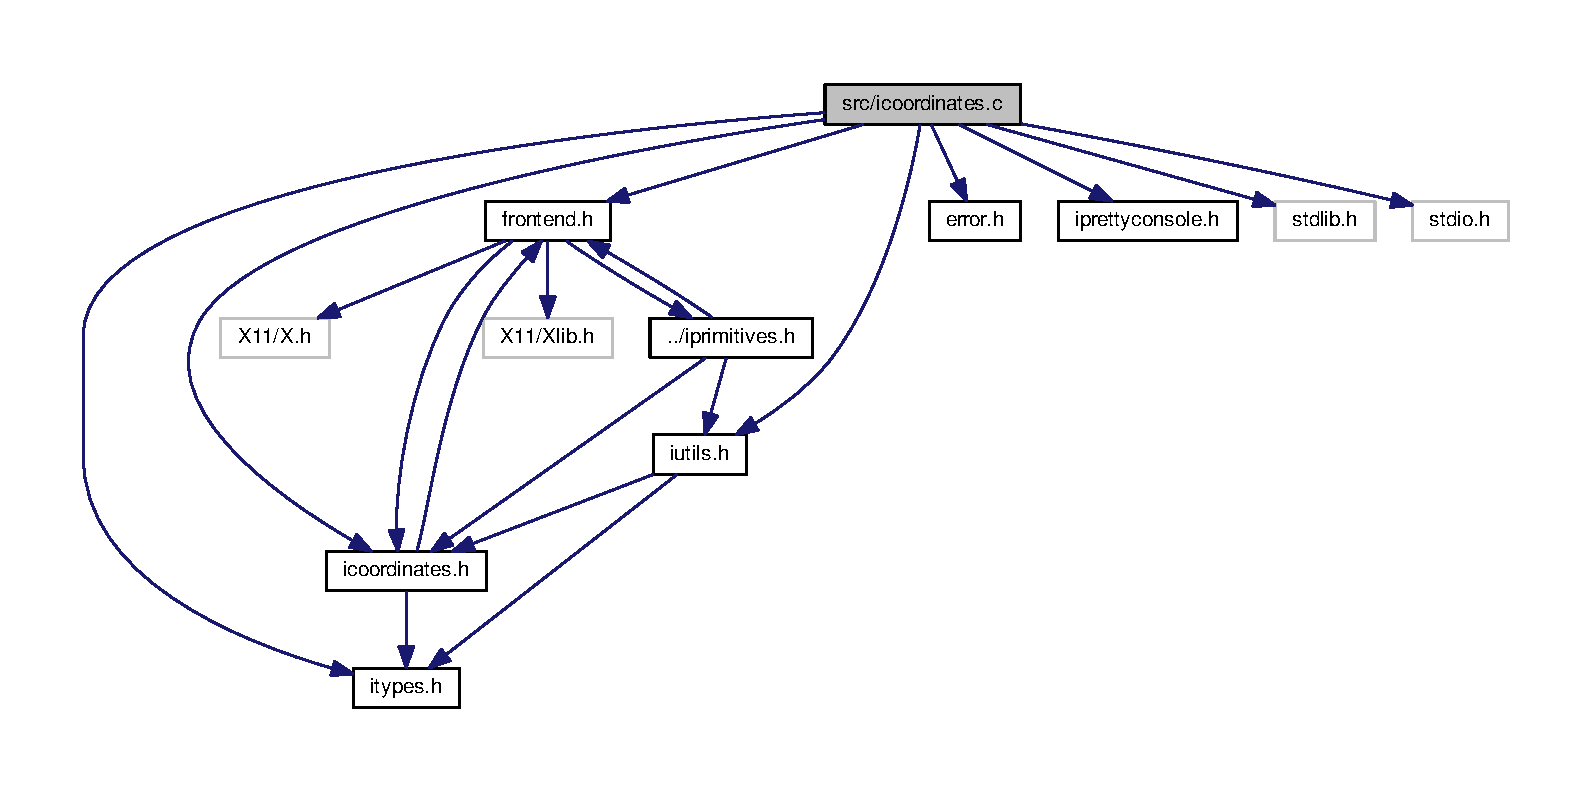
\includegraphics[width=350pt]{icoordinates_8c__incl}
\end{center}
\end{figure}
\subsection*{Functions}
\begin{DoxyCompactItemize}
\item 
struct \hyperlink{structilinkedpoint__t}{ilinkedpoint\-\_\-t} $\ast$ \hyperlink{icoordinates_8c_a7c978730cf6130f65e3ca306b83d953b}{inew\-\_\-linkedpoint} (struct \hyperlink{structipoint__t}{ipoint\-\_\-t} $\ast$point)
\item 
struct \hyperlink{structilinkedpoint__t}{ilinkedpoint\-\_\-t} $\ast$ \hyperlink{icoordinates_8c_a1576e4429e977b28e65001af937bcf3e}{iadd\-\_\-linkedpoint} (struct \hyperlink{structilinkedpoint__t}{ilinkedpoint\-\_\-t} $\ast$head, struct \hyperlink{structilinkedpoint__t}{ilinkedpoint\-\_\-t} $\ast$point)
\item 
struct \hyperlink{structilinkedpoint__t}{ilinkedpoint\-\_\-t} $\ast$ \hyperlink{icoordinates_8c_a804e459765ed24235ff910f99aa97171}{icontains\-\_\-linkedpoint} (struct \hyperlink{structilinkedpoint__t}{ilinkedpoint\-\_\-t} $\ast$head, struct \hyperlink{structilinkedpoint__t}{ilinkedpoint\-\_\-t} $\ast$lookfor)
\item 
void \hyperlink{icoordinates_8c_a6d84d9578b81bb5cf94a5bab5612c08d}{ifree\-\_\-linkedpoints} (struct \hyperlink{structilinkedpoint__t}{ilinkedpoint\-\_\-t} $\ast$head, char contents)
\item 
struct \hyperlink{structipoint__t}{ipoint\-\_\-t} $\ast$ \hyperlink{icoordinates_8c_a045ac96ebb3a6309f1fc2fd44381c45f}{inew\-\_\-point} (long double x, long double y, \hyperlink{itypes_8h_adde6aaee8457bee49c2a92621fe22b79}{uint8} z, struct \hyperlink{structifrontendstate__t}{ifrontendstate\-\_\-t} $\ast$state)
\item 
struct \hyperlink{structiabsolutepoint__t}{iabsolutepoint\-\_\-t} $\ast$ \hyperlink{icoordinates_8c_ad953c3dfb9db024d40480c2654abe255}{iget\-\_\-absolutepoint} (struct \hyperlink{structipoint__t}{ipoint\-\_\-t} $\ast$rel, struct \hyperlink{structifrontendstate__t}{ifrontendstate\-\_\-t} $\ast$state)
\item 
struct \hyperlink{structivector__t}{ivector\-\_\-t} $\ast$ \hyperlink{icoordinates_8c_a3c04cf922b23f8a788dd96261c97f50a}{inew\-\_\-vector} (double x, double y)
\item 
struct \hyperlink{structivector__t}{ivector\-\_\-t} $\ast$ \hyperlink{icoordinates_8c_ae329256a981cc3027c3945b339972130}{inormalize\-\_\-vector} (struct \hyperlink{structivector__t}{ivector\-\_\-t} $\ast$vector)
\item 
struct \hyperlink{structivector__t}{ivector\-\_\-t} $\ast$ \hyperlink{icoordinates_8c_a17716cbfb667749e45d8275b3737b33b}{ipush\-\_\-vector} (struct \hyperlink{structivector__t}{ivector\-\_\-t} $\ast$vector, struct \hyperlink{structivector__t}{ivector\-\_\-t} $\ast$direction, float magnitude)
\item 
struct \hyperlink{structivector__t}{ivector\-\_\-t} $\ast$ \hyperlink{icoordinates_8c_aa3bd0ffced71d8827c58fa3aeedad854}{iadd\-\_\-vector} (struct \hyperlink{structivector__t}{ivector\-\_\-t} $\ast$v1, struct \hyperlink{structivector__t}{ivector\-\_\-t} $\ast$v2)
\item 
void \hyperlink{icoordinates_8c_a49f0ede26f4ff04407aa27d96e333a06}{iprint\-\_\-point} (struct \hyperlink{structipoint__t}{ipoint\-\_\-t} $\ast$restrict point)
\item 
struct \hyperlink{structiregion__t}{iregion\-\_\-t} $\ast$ \hyperlink{icoordinates_8c_a4507e51c1f2470e19e8ff5a77adf54bd}{icreate\-\_\-region} (int x, int y, \hyperlink{itypes_8h_a1134b580f8da4de94ca6b1de4d37975e}{uint32} width, \hyperlink{itypes_8h_a1134b580f8da4de94ca6b1de4d37975e}{uint32} height, struct \hyperlink{structifrontendstate__t}{ifrontendstate\-\_\-t} $\ast$state)
\item 
void \hyperlink{icoordinates_8c_af824fb9002b49e7348de15d84229e536}{iprint\-\_\-vector} (struct \hyperlink{structivector__t}{ivector\-\_\-t} $\ast$restrict vec)
\item 
static size\-\_\-t \hyperlink{icoordinates_8c_a6725eb7fd1dc248c96ec9cfc949aab4e}{str\-\_\-len} (char $\ast$string)
\item 
char $\ast$ \hyperlink{icoordinates_8c_a7fb9a1c5a40e8901d93703d1006694f9}{iprints\-\_\-point} (struct \hyperlink{structipoint__t}{ipoint\-\_\-t} $\ast$restrict point)
\end{DoxyCompactItemize}


\subsection{Function Documentation}
\hypertarget{icoordinates_8c_a1576e4429e977b28e65001af937bcf3e}{\index{icoordinates.\-c@{icoordinates.\-c}!iadd\-\_\-linkedpoint@{iadd\-\_\-linkedpoint}}
\index{iadd\-\_\-linkedpoint@{iadd\-\_\-linkedpoint}!icoordinates.c@{icoordinates.\-c}}
\subsubsection[{iadd\-\_\-linkedpoint}]{\setlength{\rightskip}{0pt plus 5cm}struct {\bf ilinkedpoint\-\_\-t}$\ast$ iadd\-\_\-linkedpoint (
\begin{DoxyParamCaption}
\item[{struct {\bf ilinkedpoint\-\_\-t} $\ast$}]{head, }
\item[{struct {\bf ilinkedpoint\-\_\-t} $\ast$}]{point}
\end{DoxyParamCaption}
)}}\label{icoordinates_8c_a1576e4429e977b28e65001af937bcf3e}
add a new point to a linked points structure 
\begin{DoxyParams}{Parameters}
{\em $\ast$head} & the structure we want to append to \\
\hline
{\em $\ast$point} & the point to be appended \\
\hline
\end{DoxyParams}
\begin{DoxyReturn}{Returns}
a pointer to the new head of the list 
\end{DoxyReturn}


Definition at line 41 of file icoordinates.\-c.


\begin{DoxyCode}
42 \{
43         \textcolor{keywordflow}{if} (head) \{
44                 \textcolor{keywordflow}{if} (point) \{
45 \textcolor{preprocessor}{#if I\_PRESERVE\_LINKED\_POINTS\_ORDER==1}
46 \textcolor{preprocessor}{}                        \hyperlink{structilinkedpoint__t}{ilinkedpoint\_t} *tmp = head;
47                         \textcolor{keywordflow}{while} (head->\hyperlink{structilinkedpoint__t_a3af3bf37f168b5b11fce11262286d6c4}{next} != NULL)
48                                 head = head->\hyperlink{structilinkedpoint__t_a3af3bf37f168b5b11fce11262286d6c4}{next};
49                         head->\hyperlink{structilinkedpoint__t_a3af3bf37f168b5b11fce11262286d6c4}{next} = point;
50                         \textcolor{keywordflow}{return} tmp;
51 \textcolor{preprocessor}{#else}
52 \textcolor{preprocessor}{}                        \textcolor{keyword}{struct }\hyperlink{structilinkedpoint__t}{ilinkedpoint\_t} *tmp = head->\hyperlink{structilinkedpoint__t_a3af3bf37f168b5b11fce11262286d6c4}{next};
53                         head->\hyperlink{structilinkedpoint__t_a3af3bf37f168b5b11fce11262286d6c4}{next} = \hyperlink{structilinkedpoint__t_ad679b26e2151ec3a4ad7b062679fd3c3}{point};
54                         point->\hyperlink{structilinkedpoint__t_a3af3bf37f168b5b11fce11262286d6c4}{next} = tmp;
55                         \textcolor{keywordflow}{return} head;
56 \textcolor{preprocessor}{#endif}
57 \textcolor{preprocessor}{}                \}
58                 \hyperlink{error_8c_ab10bea042bb9daa7a0e027197b8080e5}{ierror}(\hyperlink{error_8h_a06fc87d81c62e9abb8790b6e5713c55ba0155494d2502d24c87bdcab2830802de}{I\_NULL\_LINKED\_ERROR});
59                 \textcolor{keywordflow}{return} head;
60         \}
61         \textcolor{keywordflow}{return} \hyperlink{structilinkedpoint__t_ad679b26e2151ec3a4ad7b062679fd3c3}{point};
62 \}
\end{DoxyCode}


Here is the call graph for this function\-:\nopagebreak
\begin{figure}[H]
\begin{center}
\leavevmode
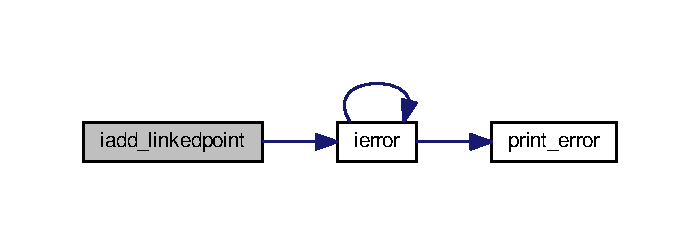
\includegraphics[width=336pt]{icoordinates_8c_a1576e4429e977b28e65001af937bcf3e_cgraph}
\end{center}
\end{figure}




Here is the caller graph for this function\-:\nopagebreak
\begin{figure}[H]
\begin{center}
\leavevmode
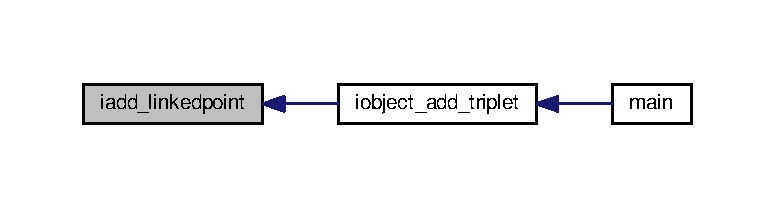
\includegraphics[width=350pt]{icoordinates_8c_a1576e4429e977b28e65001af937bcf3e_icgraph}
\end{center}
\end{figure}


\hypertarget{icoordinates_8c_aa3bd0ffced71d8827c58fa3aeedad854}{\index{icoordinates.\-c@{icoordinates.\-c}!iadd\-\_\-vector@{iadd\-\_\-vector}}
\index{iadd\-\_\-vector@{iadd\-\_\-vector}!icoordinates.c@{icoordinates.\-c}}
\subsubsection[{iadd\-\_\-vector}]{\setlength{\rightskip}{0pt plus 5cm}struct {\bf ivector\-\_\-t}$\ast$ iadd\-\_\-vector (
\begin{DoxyParamCaption}
\item[{struct {\bf ivector\-\_\-t} $\ast$}]{v1, }
\item[{struct {\bf ivector\-\_\-t} $\ast$}]{v2}
\end{DoxyParamCaption}
)}}\label{icoordinates_8c_aa3bd0ffced71d8827c58fa3aeedad854}
performs simple vector addition, v1 += v2 
\begin{DoxyParams}{Parameters}
{\em $\ast$v1} & a pointer to the destination vector \\
\hline
{\em $\ast$v2} & a pointer to the source vector \\
\hline
\end{DoxyParams}


Definition at line 210 of file icoordinates.\-c.


\begin{DoxyCode}
211 \{
212         v1->\hyperlink{structivector__t_a4b91a8fcb6a98d2ba8e2f5d483d7c577}{x} += v2->\hyperlink{structivector__t_a4b91a8fcb6a98d2ba8e2f5d483d7c577}{x};
213         v1->\hyperlink{structivector__t_af6af8ee13897aea97b1d8fe42bb83b17}{y} += v2->\hyperlink{structivector__t_af6af8ee13897aea97b1d8fe42bb83b17}{y};
214         \textcolor{keywordflow}{return} v1;
215 \}
\end{DoxyCode}
\hypertarget{icoordinates_8c_a804e459765ed24235ff910f99aa97171}{\index{icoordinates.\-c@{icoordinates.\-c}!icontains\-\_\-linkedpoint@{icontains\-\_\-linkedpoint}}
\index{icontains\-\_\-linkedpoint@{icontains\-\_\-linkedpoint}!icoordinates.c@{icoordinates.\-c}}
\subsubsection[{icontains\-\_\-linkedpoint}]{\setlength{\rightskip}{0pt plus 5cm}struct {\bf ilinkedpoint\-\_\-t}$\ast$ icontains\-\_\-linkedpoint (
\begin{DoxyParamCaption}
\item[{struct {\bf ilinkedpoint\-\_\-t} $\ast$}]{head, }
\item[{struct {\bf ilinkedpoint\-\_\-t} $\ast$}]{lookfor}
\end{DoxyParamCaption}
)}}\label{icoordinates_8c_a804e459765ed24235ff910f99aa97171}
See if an ilinkedpoint list contains a point at the same location or with the same value as a given argument. 
\begin{DoxyParams}{Parameters}
{\em $\ast$head} & The presumed \char`\"{}head\char`\"{} of the list \\
\hline
{\em $\ast$lookfor} & A pointer to the point to search for \\
\hline
\end{DoxyParams}
\begin{DoxyReturn}{Returns}
a pointer to the linked list element containing $\ast$lookfor, or N\-U\-L\-L if $\ast$lookfor can't be found in the list 
\end{DoxyReturn}


Definition at line 71 of file icoordinates.\-c.


\begin{DoxyCode}
72 \{
73         \textcolor{keywordflow}{if} (lookfor == NULL || head == NULL)
74                 \textcolor{keywordflow}{return} NULL;
75         \textcolor{keyword}{struct }\hyperlink{structilinkedpoint__t}{ilinkedpoint\_t} *hd = head;
76         \textcolor{keyword}{struct }\hyperlink{structipoint__t}{ipoint\_t} *point = lookfor->\hyperlink{structilinkedpoint__t_ad679b26e2151ec3a4ad7b062679fd3c3}{point};
77         \textcolor{keywordflow}{if} (point == NULL)
78                 \textcolor{keywordflow}{return} NULL;
79         \textcolor{keywordflow}{while} (hd) \{
80                 \textcolor{keywordflow}{if} (hd == lookfor)
81                         \textcolor{keywordflow}{return} hd;
82                 \textcolor{keywordflow}{if} (hd == NULL)
83                         \textcolor{keywordflow}{return} NULL;
84                 \textcolor{keywordflow}{if} (hd->\hyperlink{structilinkedpoint__t_ad679b26e2151ec3a4ad7b062679fd3c3}{point} == NULL)
85                         \textcolor{keywordflow}{return} NULL;
86                 \textcolor{keywordflow}{if} (point->\hyperlink{structipoint__t_a345608e139b0709cc281139e3ed6328d}{x} == ((\textcolor{keyword}{struct} \hyperlink{structipoint__t}{ipoint\_t}*)(hd->\hyperlink{structilinkedpoint__t_ad679b26e2151ec3a4ad7b062679fd3c3}{point}))->x
87                         && point->\hyperlink{structipoint__t_a88ca543f1508de060b4738cfebb51b04}{y} == hd->\hyperlink{structilinkedpoint__t_ad679b26e2151ec3a4ad7b062679fd3c3}{point}->\hyperlink{structipoint__t_a88ca543f1508de060b4738cfebb51b04}{y}
88                         && point->\hyperlink{structipoint__t_ad1680bc07190dabf544e86824b82e44b}{z} == hd->\hyperlink{structilinkedpoint__t_ad679b26e2151ec3a4ad7b062679fd3c3}{point}->\hyperlink{structipoint__t_ad1680bc07190dabf544e86824b82e44b}{z})
89                         \textcolor{keywordflow}{return} hd;
90                 hd = hd->\hyperlink{structilinkedpoint__t_a3af3bf37f168b5b11fce11262286d6c4}{next};
91         \}
92         \textcolor{keywordflow}{return} NULL;
93 \}
\end{DoxyCode}


Here is the caller graph for this function\-:\nopagebreak
\begin{figure}[H]
\begin{center}
\leavevmode
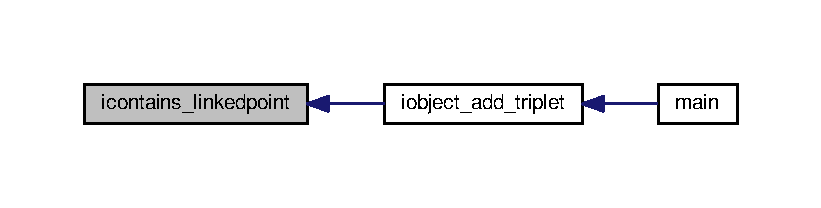
\includegraphics[width=350pt]{icoordinates_8c_a804e459765ed24235ff910f99aa97171_icgraph}
\end{center}
\end{figure}


\hypertarget{icoordinates_8c_a4507e51c1f2470e19e8ff5a77adf54bd}{\index{icoordinates.\-c@{icoordinates.\-c}!icreate\-\_\-region@{icreate\-\_\-region}}
\index{icreate\-\_\-region@{icreate\-\_\-region}!icoordinates.c@{icoordinates.\-c}}
\subsubsection[{icreate\-\_\-region}]{\setlength{\rightskip}{0pt plus 5cm}struct {\bf iregion\-\_\-t}$\ast$ icreate\-\_\-region (
\begin{DoxyParamCaption}
\item[{int}]{x, }
\item[{int}]{y, }
\item[{{\bf uint32}}]{width, }
\item[{{\bf uint32}}]{height, }
\item[{struct {\bf ifrontendstate\-\_\-t} $\ast$}]{state}
\end{DoxyParamCaption}
)}}\label{icoordinates_8c_a4507e51c1f2470e19e8ff5a77adf54bd}


Definition at line 230 of file icoordinates.\-c.


\begin{DoxyCode}
231 \{
232         \textcolor{keyword}{struct }\hyperlink{structiregion__t}{iregion\_t} *region = malloc(\textcolor{keyword}{sizeof}(\textcolor{keyword}{struct} \hyperlink{structiregion__t}{iregion\_t}));
233         region->\hyperlink{structiregion__t_a244884f21e4d054538530e389755ac3e}{x} = \hyperlink{structiregion__t_a244884f21e4d054538530e389755ac3e}{x};
234         region->\hyperlink{structiregion__t_a8b975f923a92e3969b4aec3d935af310}{y} = \hyperlink{structiregion__t_a8b975f923a92e3969b4aec3d935af310}{y};
235         region->\hyperlink{structiregion__t_abcafee0857bd757384813e53ddf879d9}{width} = \hyperlink{structiregion__t_abcafee0857bd757384813e53ddf879d9}{width};
236         region->\hyperlink{structiregion__t_ac7c841eeb48c334a9a7182480855d251}{height} = \hyperlink{structiregion__t_ac7c841eeb48c334a9a7182480855d251}{height};
237 
238         \textcolor{keywordflow}{if} (state->\hyperlink{structifrontendstate__t_a42ce77321ecea4fde68dd68b7f0f2283}{regions} == NULL) \{
239                 region->\hyperlink{structiregion__t_a09ef2d2779286827357a7c3290e65d9a}{id} = 0;
240                 state->\hyperlink{structifrontendstate__t_a42ce77321ecea4fde68dd68b7f0f2283}{regions} = \hyperlink{iutils_8c_a168fc457c8928038cb3c471bc5fdf170}{inew\_linked}(region);
241                 state->\hyperlink{structifrontendstate__t_ad30593dd0b69372008108075c55cfe27}{num\_regions} = 1;
242         \} \textcolor{keywordflow}{else} \{
243                 \hyperlink{itypes_8h_a05f6b0ae8f6a6e135b0e290c25fe0e4e}{uint16} \hyperlink{structiregion__t_a09ef2d2779286827357a7c3290e65d9a}{id};
244                 \textcolor{keyword}{struct }\hyperlink{structilinked__t}{ilinked\_t} *cur = \hyperlink{iutils_8c_acf8aca63685fbd6b4c995516baedab14}{igetfirst\_linked}(state->
      \hyperlink{structifrontendstate__t_a42ce77321ecea4fde68dd68b7f0f2283}{regions});
245                 \textcolor{keywordflow}{for} (\textcolor{keywordtype}{id} = 0; cur != NULL; cur = cur->\hyperlink{structilinked__t_ad3f173c464d58934b12da4eca2ff83f8}{next})
246                         \textcolor{keywordflow}{if} (((\textcolor{keyword}{struct} \hyperlink{structiregion__t}{iregion\_t}*)(cur->\hyperlink{structilinked__t_ac285ea385953cbd5a332b2cbab39b62b}{data}))->id > \textcolor{keywordtype}{id})
247                                 \textcolor{keywordtype}{id} = ((\textcolor{keyword}{struct }\hyperlink{structiregion__t}{iregion\_t}*)(cur->\hyperlink{structilinked__t_ac285ea385953cbd5a332b2cbab39b62b}{data}))->\textcolor{keywordtype}{id};
248                 \textcolor{keywordtype}{id} = \textcolor{keywordtype}{id} + 1;
249                 region->\hyperlink{structiregion__t_a09ef2d2779286827357a7c3290e65d9a}{id} = \hyperlink{structiregion__t_a09ef2d2779286827357a7c3290e65d9a}{id};
250                 \hyperlink{iutils_8c_a67413257923db7c88d91a7e706024e98}{iadd\_linked}(state->\hyperlink{structifrontendstate__t_a42ce77321ecea4fde68dd68b7f0f2283}{regions}, \hyperlink{iutils_8c_a168fc457c8928038cb3c471bc5fdf170}{inew\_linked}(region));
251                 state->\hyperlink{structifrontendstate__t_ad30593dd0b69372008108075c55cfe27}{num\_regions}++;
252         \}
253         \textcolor{keywordflow}{return} region;
254 \}
\end{DoxyCode}


Here is the call graph for this function\-:\nopagebreak
\begin{figure}[H]
\begin{center}
\leavevmode
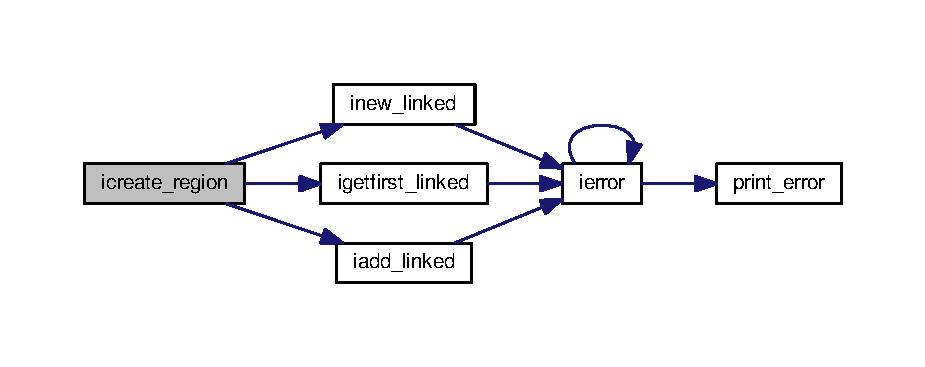
\includegraphics[width=350pt]{icoordinates_8c_a4507e51c1f2470e19e8ff5a77adf54bd_cgraph}
\end{center}
\end{figure}




Here is the caller graph for this function\-:\nopagebreak
\begin{figure}[H]
\begin{center}
\leavevmode
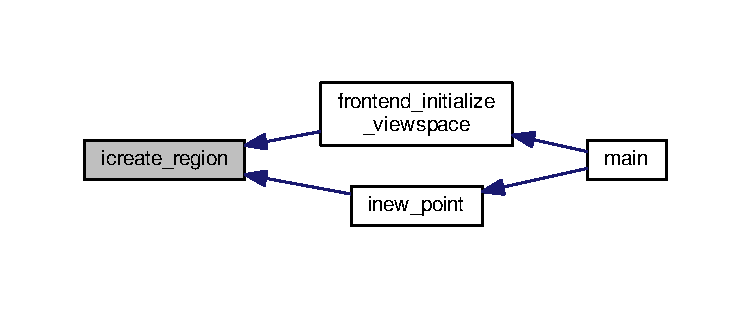
\includegraphics[width=350pt]{icoordinates_8c_a4507e51c1f2470e19e8ff5a77adf54bd_icgraph}
\end{center}
\end{figure}


\hypertarget{icoordinates_8c_a6d84d9578b81bb5cf94a5bab5612c08d}{\index{icoordinates.\-c@{icoordinates.\-c}!ifree\-\_\-linkedpoints@{ifree\-\_\-linkedpoints}}
\index{ifree\-\_\-linkedpoints@{ifree\-\_\-linkedpoints}!icoordinates.c@{icoordinates.\-c}}
\subsubsection[{ifree\-\_\-linkedpoints}]{\setlength{\rightskip}{0pt plus 5cm}void ifree\-\_\-linkedpoints (
\begin{DoxyParamCaption}
\item[{struct {\bf ilinkedpoint\-\_\-t} $\ast$}]{head, }
\item[{char}]{contents}
\end{DoxyParamCaption}
)}}\label{icoordinates_8c_a6d84d9578b81bb5cf94a5bab5612c08d}
free a linkedpoint list 
\begin{DoxyParams}{Parameters}
{\em $\ast$head} & The head of the list \\
\hline
{\em contents} & determine if the points \char`\"{}contained\char`\"{} in the list should be freed as well. 'y' or 1 mean \char`\"{}yes\char`\"{} and 'n' or '0' mean \char`\"{}no\char`\"{}. \\
\hline
\end{DoxyParams}


Definition at line 100 of file icoordinates.\-c.


\begin{DoxyCode}
101 \{
102         \textcolor{keyword}{struct }\hyperlink{structilinkedpoint__t}{ilinkedpoint\_t} *tmp = head->\hyperlink{structilinkedpoint__t_a3af3bf37f168b5b11fce11262286d6c4}{next};
103         \textcolor{keywordflow}{while} (head) \{
104                 \textcolor{keywordflow}{if} (contents == \textcolor{charliteral}{'y'}) \{
105                         free(head->\hyperlink{structilinkedpoint__t_ad679b26e2151ec3a4ad7b062679fd3c3}{point});
106                 \}
107                 free(head);
108                 head = tmp;
109                 tmp = head->\hyperlink{structilinkedpoint__t_a3af3bf37f168b5b11fce11262286d6c4}{next};
110         \}
111 \}
\end{DoxyCode}


Here is the caller graph for this function\-:\nopagebreak
\begin{figure}[H]
\begin{center}
\leavevmode
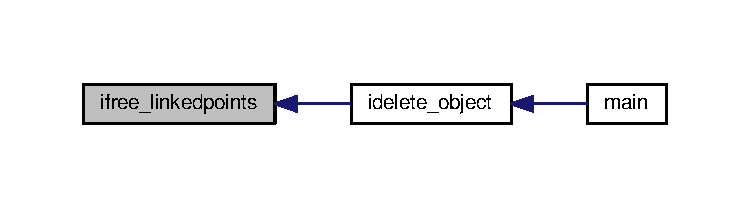
\includegraphics[width=350pt]{icoordinates_8c_a6d84d9578b81bb5cf94a5bab5612c08d_icgraph}
\end{center}
\end{figure}


\hypertarget{icoordinates_8c_ad953c3dfb9db024d40480c2654abe255}{\index{icoordinates.\-c@{icoordinates.\-c}!iget\-\_\-absolutepoint@{iget\-\_\-absolutepoint}}
\index{iget\-\_\-absolutepoint@{iget\-\_\-absolutepoint}!icoordinates.c@{icoordinates.\-c}}
\subsubsection[{iget\-\_\-absolutepoint}]{\setlength{\rightskip}{0pt plus 5cm}struct {\bf iabsolutepoint\-\_\-t}$\ast$ iget\-\_\-absolutepoint (
\begin{DoxyParamCaption}
\item[{struct {\bf ipoint\-\_\-t} $\ast$}]{rel, }
\item[{struct {\bf ifrontendstate\-\_\-t} $\ast$}]{state}
\end{DoxyParamCaption}
)}}\label{icoordinates_8c_ad953c3dfb9db024d40480c2654abe255}


Definition at line 174 of file icoordinates.\-c.


\begin{DoxyCode}
175 \{
176         \textcolor{keyword}{struct }\hyperlink{structiabsolutepoint__t}{iabsolutepoint\_t} *rval = malloc(\textcolor{keyword}{sizeof}(\textcolor{keyword}{struct} 
      \hyperlink{structiabsolutepoint__t}{iabsolutepoint\_t}));
177         rval->\hyperlink{structiabsolutepoint__t_a7c546cbece73b64e924b982d1647005f}{x} = rel->\hyperlink{structipoint__t_a345608e139b0709cc281139e3ed6328d}{x};
178         rval->\hyperlink{structiabsolutepoint__t_a12ea188889c536abe1c6eba40dc62c39}{y} = rel->\hyperlink{structipoint__t_a88ca543f1508de060b4738cfebb51b04}{y};
179         \textcolor{comment}{//rval->x += (long double)}
180         \textcolor{comment}{//}
181         \textcolor{keywordflow}{return} rval;
182 \}
\end{DoxyCode}
\hypertarget{icoordinates_8c_a7c978730cf6130f65e3ca306b83d953b}{\index{icoordinates.\-c@{icoordinates.\-c}!inew\-\_\-linkedpoint@{inew\-\_\-linkedpoint}}
\index{inew\-\_\-linkedpoint@{inew\-\_\-linkedpoint}!icoordinates.c@{icoordinates.\-c}}
\subsubsection[{inew\-\_\-linkedpoint}]{\setlength{\rightskip}{0pt plus 5cm}struct {\bf ilinkedpoint\-\_\-t}$\ast$ inew\-\_\-linkedpoint (
\begin{DoxyParamCaption}
\item[{struct {\bf ipoint\-\_\-t} $\ast$}]{point}
\end{DoxyParamCaption}
)}}\label{icoordinates_8c_a7c978730cf6130f65e3ca306b83d953b}
allocate and initialize a new ilinkedpoint structure, a type of singly linked list specialized for holding ipoints 
\begin{DoxyParams}{Parameters}
{\em $\ast$point} & the ipoint structure the be \char`\"{}contained\char`\"{} the the link \\
\hline
\end{DoxyParams}
\begin{DoxyReturn}{Returns}
the new ilinkedpoint, or N\-U\-L\-L on failure 
\end{DoxyReturn}


Definition at line 20 of file icoordinates.\-c.


\begin{DoxyCode}
21 \{
22         \textcolor{keywordflow}{if} (point) \{
23                 \textcolor{keyword}{struct }\hyperlink{structilinkedpoint__t}{ilinkedpoint\_t} *rval = malloc(\textcolor{keyword}{sizeof}(\textcolor{keyword}{struct} 
      \hyperlink{structilinkedpoint__t}{ilinkedpoint\_t}));
24                 \textcolor{keywordflow}{if} (rval) \{
25                         rval->\hyperlink{structilinkedpoint__t_a3af3bf37f168b5b11fce11262286d6c4}{next} = NULL;
26                         rval->\hyperlink{structilinkedpoint__t_ad679b26e2151ec3a4ad7b062679fd3c3}{point} = \hyperlink{structilinkedpoint__t_ad679b26e2151ec3a4ad7b062679fd3c3}{point};
27                         \textcolor{keywordflow}{return} rval;
28                 \}
29                 \hyperlink{error_8c_ab10bea042bb9daa7a0e027197b8080e5}{ierror}(\hyperlink{error_8h_a06fc87d81c62e9abb8790b6e5713c55bac52ce3dc72e9de7cd173594b72138a02}{I\_INITIALIZATION\_ERROR});
30                 \textcolor{keywordflow}{return} NULL;
31         \}
32         \hyperlink{error_8c_ab10bea042bb9daa7a0e027197b8080e5}{ierror}(\hyperlink{error_8h_a06fc87d81c62e9abb8790b6e5713c55ba0155494d2502d24c87bdcab2830802de}{I\_NULL\_LINKED\_ERROR});
33         \textcolor{keywordflow}{return} NULL;
34 \}
\end{DoxyCode}


Here is the call graph for this function\-:\nopagebreak
\begin{figure}[H]
\begin{center}
\leavevmode
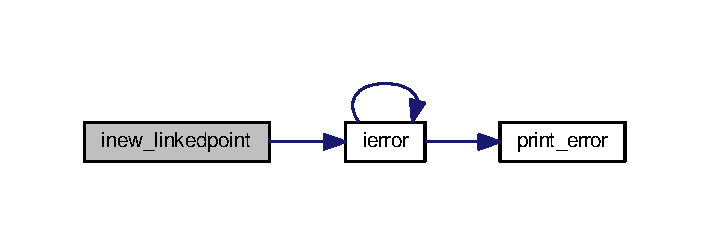
\includegraphics[width=340pt]{icoordinates_8c_a7c978730cf6130f65e3ca306b83d953b_cgraph}
\end{center}
\end{figure}




Here is the caller graph for this function\-:\nopagebreak
\begin{figure}[H]
\begin{center}
\leavevmode
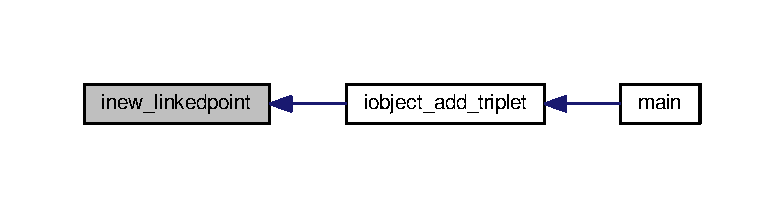
\includegraphics[width=350pt]{icoordinates_8c_a7c978730cf6130f65e3ca306b83d953b_icgraph}
\end{center}
\end{figure}


\hypertarget{icoordinates_8c_a045ac96ebb3a6309f1fc2fd44381c45f}{\index{icoordinates.\-c@{icoordinates.\-c}!inew\-\_\-point@{inew\-\_\-point}}
\index{inew\-\_\-point@{inew\-\_\-point}!icoordinates.c@{icoordinates.\-c}}
\subsubsection[{inew\-\_\-point}]{\setlength{\rightskip}{0pt plus 5cm}struct {\bf ipoint\-\_\-t}$\ast$ inew\-\_\-point (
\begin{DoxyParamCaption}
\item[{long double}]{x, }
\item[{long double}]{y, }
\item[{{\bf uint8}}]{z, }
\item[{struct {\bf ifrontendstate\-\_\-t} $\ast$}]{state}
\end{DoxyParamCaption}
)}}\label{icoordinates_8c_a045ac96ebb3a6309f1fc2fd44381c45f}
Allocates and initializes a new point using the new region system 

Definition at line 116 of file icoordinates.\-c.


\begin{DoxyCode}
117 \{
118         \textcolor{keyword}{struct }\hyperlink{structipoint__t}{ipoint\_t} *rval = malloc(\textcolor{keyword}{sizeof}(\textcolor{keyword}{struct} \hyperlink{structipoint__t}{ipoint\_t}));
119         \textcolor{keywordflow}{if} (state == NULL) \{
120                 rval->\hyperlink{structipoint__t_a345608e139b0709cc281139e3ed6328d}{x} = \hyperlink{structipoint__t_a345608e139b0709cc281139e3ed6328d}{x};
121                 rval->\hyperlink{structipoint__t_a88ca543f1508de060b4738cfebb51b04}{y} = \hyperlink{structipoint__t_a88ca543f1508de060b4738cfebb51b04}{y};
122                 rval->\hyperlink{structipoint__t_ad1680bc07190dabf544e86824b82e44b}{z} = \hyperlink{structipoint__t_ad1680bc07190dabf544e86824b82e44b}{z};
123                 rval->\hyperlink{structipoint__t_a92092dc10d022e8cbeea97795e16f55b}{region} = -1;
124                 \textcolor{keywordflow}{return} rval;
125         \}
126         \textcolor{keyword}{volatile} \textcolor{keyword}{struct }\hyperlink{structilinked__t}{ilinked\_t} *list = \hyperlink{iutils_8c_acf8aca63685fbd6b4c995516baedab14}{igetfirst\_linked}(state->
      \hyperlink{structifrontendstate__t_a42ce77321ecea4fde68dd68b7f0f2283}{regions});
127         \textcolor{keyword}{volatile} \textcolor{keyword}{struct }\hyperlink{structiregion__t}{iregion\_t} *region;
128 
129         \textcolor{keywordtype}{long} \textcolor{keywordtype}{int} \_x = (\textcolor{keywordtype}{long} int)\hyperlink{structiregion__t_a244884f21e4d054538530e389755ac3e}{x}, \_y = (\textcolor{keywordtype}{long} \textcolor{keywordtype}{int})\hyperlink{structiregion__t_a8b975f923a92e3969b4aec3d935af310}{y};
130 
131         \textcolor{keywordflow}{if} (list == NULL)
132                 \textcolor{keywordflow}{goto} HANDLE\_NO\_VALID\_REGIONS;
133 
134         \textcolor{keywordflow}{for} ( ; list != NULL; list = list->\hyperlink{structilinked__t_ad3f173c464d58934b12da4eca2ff83f8}{next}) \{
135                 region = (\textcolor{keyword}{struct }\hyperlink{structiregion__t}{iregion\_t}*)(list->\hyperlink{structilinked__t_ac285ea385953cbd5a332b2cbab39b62b}{data});
136                 \textcolor{keywordflow}{if} (\hyperlink{structiregion__t_a244884f21e4d054538530e389755ac3e}{x} > region->\hyperlink{structiregion__t_a244884f21e4d054538530e389755ac3e}{x} && x < region->\hyperlink{structiregion__t_a244884f21e4d054538530e389755ac3e}{x} + region->\hyperlink{structiregion__t_abcafee0857bd757384813e53ddf879d9}{width})
137                         \textcolor{keywordflow}{if} (\hyperlink{structiregion__t_a8b975f923a92e3969b4aec3d935af310}{y} > region->\hyperlink{structiregion__t_a8b975f923a92e3969b4aec3d935af310}{y} && y < region->\hyperlink{structiregion__t_a8b975f923a92e3969b4aec3d935af310}{y} + region->\hyperlink{structiregion__t_ac7c841eeb48c334a9a7182480855d251}{height}) \{
138                                 rval->\hyperlink{structipoint__t_a92092dc10d022e8cbeea97795e16f55b}{region} = region->\hyperlink{structiregion__t_a09ef2d2779286827357a7c3290e65d9a}{id};
139                                 \textcolor{keywordflow}{break};
140                         \}
141         \}
142         \textcolor{keywordflow}{if} (list == NULL) \{
143 HANDLE\_NO\_VALID\_REGIONS:
144                 \textcolor{keywordflow}{if} (\hyperlink{structiregion__t_a244884f21e4d054538530e389755ac3e}{x} > 0)
145                         \_x = \_x - \_x % \hyperlink{icoordinates_8h_ac1de6770b93fc86eda03aca4bb9183e0}{DEFAULT\_REGION\_WIDTH};
146                 \textcolor{keywordflow}{else} \textcolor{keywordflow}{if} (\hyperlink{structiregion__t_a244884f21e4d054538530e389755ac3e}{x} < 0)
147                         \_x = \_x - (\hyperlink{icoordinates_8h_ac1de6770b93fc86eda03aca4bb9183e0}{DEFAULT\_REGION\_WIDTH} + (\_x % 
      \hyperlink{icoordinates_8h_ac1de6770b93fc86eda03aca4bb9183e0}{DEFAULT\_REGION\_WIDTH}));
148                 \textcolor{keywordflow}{else}
149                         \_x = 0;
150 
151                 \textcolor{keywordflow}{if} (\hyperlink{structiregion__t_a8b975f923a92e3969b4aec3d935af310}{y} > 0)
152                         \_y = \_y - \_y % \hyperlink{icoordinates_8h_ae7530daba46f50a0254f51d8a66f75bd}{DEFAULT\_REGION\_HEIGHT};
153                 \textcolor{keywordflow}{else} \textcolor{keywordflow}{if} (\hyperlink{structiregion__t_a8b975f923a92e3969b4aec3d935af310}{y} < 0)
154                         \_y = \_y - (\hyperlink{icoordinates_8h_ae7530daba46f50a0254f51d8a66f75bd}{DEFAULT\_REGION\_HEIGHT} + (\_y % 
      \hyperlink{icoordinates_8h_ae7530daba46f50a0254f51d8a66f75bd}{DEFAULT\_REGION\_HEIGHT}));
155                 \textcolor{keywordflow}{else}
156                         \_y = 0;
157                 
158                 \textcolor{keyword}{struct }\hyperlink{structiregion__t}{iregion\_t} *newregion = NULL;
159                 newregion = \hyperlink{icoordinates_8c_a4507e51c1f2470e19e8ff5a77adf54bd}{icreate\_region}(\_x, \_y, 
      \hyperlink{icoordinates_8h_ac1de6770b93fc86eda03aca4bb9183e0}{DEFAULT\_REGION\_WIDTH},
160                                                    \hyperlink{icoordinates_8h_ae7530daba46f50a0254f51d8a66f75bd}{DEFAULT\_REGION\_HEIGHT}, state);
161 
162                 region = newregion;
163         \}
164         rval->\hyperlink{structipoint__t_a92092dc10d022e8cbeea97795e16f55b}{region} = region->\hyperlink{structiregion__t_a09ef2d2779286827357a7c3290e65d9a}{id};
165         rval->\hyperlink{structipoint__t_a345608e139b0709cc281139e3ed6328d}{x} = \hyperlink{structiregion__t_a244884f21e4d054538530e389755ac3e}{x} - (\textcolor{keywordtype}{long} double)(region->\hyperlink{structiregion__t_a244884f21e4d054538530e389755ac3e}{x});
166         rval->\hyperlink{structipoint__t_a88ca543f1508de060b4738cfebb51b04}{y} = \hyperlink{structiregion__t_a8b975f923a92e3969b4aec3d935af310}{y} - (\textcolor{keywordtype}{long} double)(region->\hyperlink{structiregion__t_a8b975f923a92e3969b4aec3d935af310}{y});
167         rval->\hyperlink{structipoint__t_ad1680bc07190dabf544e86824b82e44b}{z} = z;
168         \textcolor{keywordflow}{return} rval;
169 \}
\end{DoxyCode}


Here is the call graph for this function\-:\nopagebreak
\begin{figure}[H]
\begin{center}
\leavevmode
\includegraphics[width=350pt]{icoordinates_8c_a045ac96ebb3a6309f1fc2fd44381c45f_cgraph}
\end{center}
\end{figure}




Here is the caller graph for this function\-:\nopagebreak
\begin{figure}[H]
\begin{center}
\leavevmode
\includegraphics[width=218pt]{icoordinates_8c_a045ac96ebb3a6309f1fc2fd44381c45f_icgraph}
\end{center}
\end{figure}


\hypertarget{icoordinates_8c_a3c04cf922b23f8a788dd96261c97f50a}{\index{icoordinates.\-c@{icoordinates.\-c}!inew\-\_\-vector@{inew\-\_\-vector}}
\index{inew\-\_\-vector@{inew\-\_\-vector}!icoordinates.c@{icoordinates.\-c}}
\subsubsection[{inew\-\_\-vector}]{\setlength{\rightskip}{0pt plus 5cm}struct {\bf ivector\-\_\-t}$\ast$ inew\-\_\-vector (
\begin{DoxyParamCaption}
\item[{double}]{x, }
\item[{double}]{y}
\end{DoxyParamCaption}
)}}\label{icoordinates_8c_a3c04cf922b23f8a788dd96261c97f50a}


Definition at line 184 of file icoordinates.\-c.


\begin{DoxyCode}
185 \{
186         \textcolor{keyword}{struct }\hyperlink{structivector__t}{ivector\_t} *rval = malloc(\textcolor{keyword}{sizeof}(\textcolor{keyword}{struct} \hyperlink{structivector__t}{ivector\_t}));
187         rval->\hyperlink{structivector__t_a4b91a8fcb6a98d2ba8e2f5d483d7c577}{x} = \hyperlink{structivector__t_a4b91a8fcb6a98d2ba8e2f5d483d7c577}{x};
188         rval->\hyperlink{structivector__t_af6af8ee13897aea97b1d8fe42bb83b17}{y} = \hyperlink{structivector__t_af6af8ee13897aea97b1d8fe42bb83b17}{y};
189         \textcolor{keywordflow}{return} rval;
190 \}
\end{DoxyCode}


Here is the caller graph for this function\-:\nopagebreak
\begin{figure}[H]
\begin{center}
\leavevmode
\includegraphics[width=324pt]{icoordinates_8c_a3c04cf922b23f8a788dd96261c97f50a_icgraph}
\end{center}
\end{figure}


\hypertarget{icoordinates_8c_ae329256a981cc3027c3945b339972130}{\index{icoordinates.\-c@{icoordinates.\-c}!inormalize\-\_\-vector@{inormalize\-\_\-vector}}
\index{inormalize\-\_\-vector@{inormalize\-\_\-vector}!icoordinates.c@{icoordinates.\-c}}
\subsubsection[{inormalize\-\_\-vector}]{\setlength{\rightskip}{0pt plus 5cm}struct {\bf ivector\-\_\-t}$\ast$ inormalize\-\_\-vector (
\begin{DoxyParamCaption}
\item[{struct {\bf ivector\-\_\-t} $\ast$}]{vector}
\end{DoxyParamCaption}
)}}\label{icoordinates_8c_ae329256a981cc3027c3945b339972130}


Definition at line 192 of file icoordinates.\-c.


\begin{DoxyCode}
193 \{
194         \textcolor{keywordtype}{float} invlength = \hyperlink{iutils_8c_a1c96160b622425f63f2566171feda038}{ifast\_rsqrt}(vector->\hyperlink{structivector__t_a4b91a8fcb6a98d2ba8e2f5d483d7c577}{x} * vector->\hyperlink{structivector__t_a4b91a8fcb6a98d2ba8e2f5d483d7c577}{x} + vector->
      \hyperlink{structivector__t_af6af8ee13897aea97b1d8fe42bb83b17}{y} * vector->\hyperlink{structivector__t_af6af8ee13897aea97b1d8fe42bb83b17}{y});
195         vector->\hyperlink{structivector__t_a4b91a8fcb6a98d2ba8e2f5d483d7c577}{x} *= invlength;
196         vector->\hyperlink{structivector__t_af6af8ee13897aea97b1d8fe42bb83b17}{y} *= invlength;
197         \textcolor{keywordflow}{return} vector;
198 \}
\end{DoxyCode}


Here is the call graph for this function\-:\nopagebreak
\begin{figure}[H]
\begin{center}
\leavevmode
\includegraphics[width=270pt]{icoordinates_8c_ae329256a981cc3027c3945b339972130_cgraph}
\end{center}
\end{figure}


\hypertarget{icoordinates_8c_a49f0ede26f4ff04407aa27d96e333a06}{\index{icoordinates.\-c@{icoordinates.\-c}!iprint\-\_\-point@{iprint\-\_\-point}}
\index{iprint\-\_\-point@{iprint\-\_\-point}!icoordinates.c@{icoordinates.\-c}}
\subsubsection[{iprint\-\_\-point}]{\setlength{\rightskip}{0pt plus 5cm}void iprint\-\_\-point (
\begin{DoxyParamCaption}
\item[{struct {\bf ipoint\-\_\-t} $\ast$restrict}]{point}
\end{DoxyParamCaption}
)}}\label{icoordinates_8c_a49f0ede26f4ff04407aa27d96e333a06}
prints a point all pretty-\/like 
\begin{DoxyParams}{Parameters}
{\em $\ast$point} & the point to print \\
\hline
\end{DoxyParams}


Definition at line 220 of file icoordinates.\-c.


\begin{DoxyCode}
221 \{
222         printf(\textcolor{stringliteral}{"point "} \hyperlink{iprettyconsole_8h_a897b10d246533c95ba86cb79f92e465a}{KYEL} \textcolor{stringliteral}{"@@%p"} \hyperlink{iprettyconsole_8h_ab702106cf3b3e96750b6845ded4e0299}{RESET} \textcolor{stringliteral}{", coordinates(%f, %f, %d)\(\backslash\)n"}, (\textcolor{keywordtype}{void}*)point,
223                         point->\hyperlink{structipoint__t_a345608e139b0709cc281139e3ed6328d}{x},
224                         point->\hyperlink{structipoint__t_a88ca543f1508de060b4738cfebb51b04}{y},
225                         point->\hyperlink{structipoint__t_ad1680bc07190dabf544e86824b82e44b}{z}
226               );
227         \textcolor{keywordflow}{return};
228 \}
\end{DoxyCode}


Here is the caller graph for this function\-:\nopagebreak
\begin{figure}[H]
\begin{center}
\leavevmode
\includegraphics[width=324pt]{icoordinates_8c_a49f0ede26f4ff04407aa27d96e333a06_icgraph}
\end{center}
\end{figure}


\hypertarget{icoordinates_8c_af824fb9002b49e7348de15d84229e536}{\index{icoordinates.\-c@{icoordinates.\-c}!iprint\-\_\-vector@{iprint\-\_\-vector}}
\index{iprint\-\_\-vector@{iprint\-\_\-vector}!icoordinates.c@{icoordinates.\-c}}
\subsubsection[{iprint\-\_\-vector}]{\setlength{\rightskip}{0pt plus 5cm}void iprint\-\_\-vector (
\begin{DoxyParamCaption}
\item[{struct {\bf ivector\-\_\-t} $\ast$restrict}]{vec}
\end{DoxyParamCaption}
)}}\label{icoordinates_8c_af824fb9002b49e7348de15d84229e536}
prints a vector all pretty-\/like 
\begin{DoxyParams}{Parameters}
{\em $\ast$vec} & the vector to print \\
\hline
\end{DoxyParams}
\begin{DoxyRefDesc}{Todo}
\item[\hyperlink{todo__todo000001}{Todo}]make it prettier \end{DoxyRefDesc}


Definition at line 260 of file icoordinates.\-c.


\begin{DoxyCode}
261 \{
262         printf(\textcolor{stringliteral}{"ivector\_t @%p, (x, y) = (%lf, %lf)\(\backslash\)n"}, (\textcolor{keywordtype}{void}*)vec, vec->\hyperlink{structivector__t_a4b91a8fcb6a98d2ba8e2f5d483d7c577}{x}, vec->
      \hyperlink{structivector__t_af6af8ee13897aea97b1d8fe42bb83b17}{y});
263 \}
\end{DoxyCode}


Here is the caller graph for this function\-:\nopagebreak
\begin{figure}[H]
\begin{center}
\leavevmode
\includegraphics[width=330pt]{icoordinates_8c_af824fb9002b49e7348de15d84229e536_icgraph}
\end{center}
\end{figure}


\hypertarget{icoordinates_8c_a7fb9a1c5a40e8901d93703d1006694f9}{\index{icoordinates.\-c@{icoordinates.\-c}!iprints\-\_\-point@{iprints\-\_\-point}}
\index{iprints\-\_\-point@{iprints\-\_\-point}!icoordinates.c@{icoordinates.\-c}}
\subsubsection[{iprints\-\_\-point}]{\setlength{\rightskip}{0pt plus 5cm}char$\ast$ iprints\-\_\-point (
\begin{DoxyParamCaption}
\item[{struct {\bf ipoint\-\_\-t} $\ast$restrict}]{point}
\end{DoxyParamCaption}
)}}\label{icoordinates_8c_a7fb9a1c5a40e8901d93703d1006694f9}
prints a point all pretty-\/like to a new string 
\begin{DoxyParams}{Parameters}
{\em $\ast$point} & a pointer to the point to print \\
\hline
\end{DoxyParams}
\begin{DoxyReturn}{Returns}
a string 
\end{DoxyReturn}


Definition at line 283 of file icoordinates.\-c.


\begin{DoxyCode}
284 \{
285         \textcolor{keywordtype}{char} *buffer = malloc(64 * \textcolor{keyword}{sizeof}(\textcolor{keywordtype}{char}));
286         sprintf(buffer, \textcolor{stringliteral}{"ipoint\_t at %p, coordinates(%f, %f, %d)"},
287                         (\textcolor{keywordtype}{void}*)point,
288                         point->\hyperlink{structipoint__t_a345608e139b0709cc281139e3ed6328d}{x},
289                         point->\hyperlink{structipoint__t_a88ca543f1508de060b4738cfebb51b04}{y},
290                         point->\hyperlink{structipoint__t_ad1680bc07190dabf544e86824b82e44b}{z}
291               );
292         buffer = realloc(buffer, \hyperlink{icoordinates_8c_a6725eb7fd1dc248c96ec9cfc949aab4e}{str\_len}(buffer));
293         \textcolor{keywordflow}{return} buffer;
294 \}
\end{DoxyCode}


Here is the call graph for this function\-:\nopagebreak
\begin{figure}[H]
\begin{center}
\leavevmode
\includegraphics[width=232pt]{icoordinates_8c_a7fb9a1c5a40e8901d93703d1006694f9_cgraph}
\end{center}
\end{figure}


\hypertarget{icoordinates_8c_a17716cbfb667749e45d8275b3737b33b}{\index{icoordinates.\-c@{icoordinates.\-c}!ipush\-\_\-vector@{ipush\-\_\-vector}}
\index{ipush\-\_\-vector@{ipush\-\_\-vector}!icoordinates.c@{icoordinates.\-c}}
\subsubsection[{ipush\-\_\-vector}]{\setlength{\rightskip}{0pt plus 5cm}struct {\bf ivector\-\_\-t}$\ast$ ipush\-\_\-vector (
\begin{DoxyParamCaption}
\item[{struct {\bf ivector\-\_\-t} $\ast$}]{vector, }
\item[{struct {\bf ivector\-\_\-t} $\ast$}]{direction, }
\item[{float}]{magnitude}
\end{DoxyParamCaption}
)}}\label{icoordinates_8c_a17716cbfb667749e45d8275b3737b33b}


Definition at line 200 of file icoordinates.\-c.


\begin{DoxyCode}
201 \{
202         
203         \textcolor{keywordflow}{return} vector;
204 \}
\end{DoxyCode}
\hypertarget{icoordinates_8c_a6725eb7fd1dc248c96ec9cfc949aab4e}{\index{icoordinates.\-c@{icoordinates.\-c}!str\-\_\-len@{str\-\_\-len}}
\index{str\-\_\-len@{str\-\_\-len}!icoordinates.c@{icoordinates.\-c}}
\subsubsection[{str\-\_\-len}]{\setlength{\rightskip}{0pt plus 5cm}static size\-\_\-t str\-\_\-len (
\begin{DoxyParamCaption}
\item[{char $\ast$}]{string}
\end{DoxyParamCaption}
)\hspace{0.3cm}{\ttfamily [inline]}, {\ttfamily [static]}}}\label{icoordinates_8c_a6725eb7fd1dc248c96ec9cfc949aab4e}
a static inline homebrew strlen function so that I don't have to include the whole string.\-h header 
\begin{DoxyParams}{Parameters}
{\em $\ast$string} & the string to find the length of \\
\hline
\end{DoxyParams}
\begin{DoxyReturn}{Returns}
length of the string, in number of characters 
\end{DoxyReturn}


Definition at line 269 of file icoordinates.\-c.


\begin{DoxyCode}
273 \{
274         \textcolor{keywordtype}{size\_t} i;
275         \textcolor{keywordflow}{for} ( i = 0; *(\textcolor{keywordtype}{string} + i) != \textcolor{charliteral}{'\(\backslash\)0'}; ++i) ;
276         \textcolor{keywordflow}{return} i;
277 \}
\end{DoxyCode}


Here is the caller graph for this function\-:\nopagebreak
\begin{figure}[H]
\begin{center}
\leavevmode
\includegraphics[width=232pt]{icoordinates_8c_a6725eb7fd1dc248c96ec9cfc949aab4e_icgraph}
\end{center}
\end{figure}



\hypertarget{icoordinates_8h}{\section{src/icoordinates.h File Reference}
\label{icoordinates_8h}\index{src/icoordinates.\-h@{src/icoordinates.\-h}}
}
{\ttfamily \#include \char`\"{}frontend.\-h\char`\"{}}\\*
{\ttfamily \#include \char`\"{}itypes.\-h\char`\"{}}\\*
Include dependency graph for icoordinates.\-h\-:\nopagebreak
\begin{figure}[H]
\begin{center}
\leavevmode
\includegraphics[width=350pt]{icoordinates_8h__incl}
\end{center}
\end{figure}
This graph shows which files directly or indirectly include this file\-:
\nopagebreak
\begin{figure}[H]
\begin{center}
\leavevmode
\includegraphics[width=350pt]{icoordinates_8h__dep__incl}
\end{center}
\end{figure}
\subsection*{Data Structures}
\begin{DoxyCompactItemize}
\item 
struct \hyperlink{structiregion__t}{iregion\-\_\-t}
\item 
struct \hyperlink{structipoint__t}{ipoint\-\_\-t}
\item 
struct \hyperlink{structiabsolutepoint__t}{iabsolutepoint\-\_\-t}
\item 
struct \hyperlink{structilinkedpoint__t}{ilinkedpoint\-\_\-t}
\item 
struct \hyperlink{structivector__t}{ivector\-\_\-t}
\end{DoxyCompactItemize}
\subsection*{Macros}
\begin{DoxyCompactItemize}
\item 
\#define \hyperlink{icoordinates_8h_ac1de6770b93fc86eda03aca4bb9183e0}{D\-E\-F\-A\-U\-L\-T\-\_\-\-R\-E\-G\-I\-O\-N\-\_\-\-W\-I\-D\-T\-H}~128
\item 
\#define \hyperlink{icoordinates_8h_ae7530daba46f50a0254f51d8a66f75bd}{D\-E\-F\-A\-U\-L\-T\-\_\-\-R\-E\-G\-I\-O\-N\-\_\-\-H\-E\-I\-G\-H\-T}~128
\end{DoxyCompactItemize}
\subsection*{Functions}
\begin{DoxyCompactItemize}
\item 
struct \hyperlink{structilinkedpoint__t}{ilinkedpoint\-\_\-t} $\ast$ \hyperlink{icoordinates_8h_a7c978730cf6130f65e3ca306b83d953b}{inew\-\_\-linkedpoint} (struct \hyperlink{structipoint__t}{ipoint\-\_\-t} $\ast$point)
\item 
struct \hyperlink{structilinkedpoint__t}{ilinkedpoint\-\_\-t} $\ast$ \hyperlink{icoordinates_8h_a1576e4429e977b28e65001af937bcf3e}{iadd\-\_\-linkedpoint} (struct \hyperlink{structilinkedpoint__t}{ilinkedpoint\-\_\-t} $\ast$head, struct \hyperlink{structilinkedpoint__t}{ilinkedpoint\-\_\-t} $\ast$point)
\item 
struct \hyperlink{structilinkedpoint__t}{ilinkedpoint\-\_\-t} $\ast$ \hyperlink{icoordinates_8h_a804e459765ed24235ff910f99aa97171}{icontains\-\_\-linkedpoint} (struct \hyperlink{structilinkedpoint__t}{ilinkedpoint\-\_\-t} $\ast$head, struct \hyperlink{structilinkedpoint__t}{ilinkedpoint\-\_\-t} $\ast$lookfor)
\item 
void \hyperlink{icoordinates_8h_a6d84d9578b81bb5cf94a5bab5612c08d}{ifree\-\_\-linkedpoints} (struct \hyperlink{structilinkedpoint__t}{ilinkedpoint\-\_\-t} $\ast$head, char contents)
\item 
struct \hyperlink{structipoint__t}{ipoint\-\_\-t} $\ast$ \hyperlink{icoordinates_8h_a045ac96ebb3a6309f1fc2fd44381c45f}{inew\-\_\-point} (long double x, long double y, \hyperlink{itypes_8h_adde6aaee8457bee49c2a92621fe22b79}{uint8} z, struct \hyperlink{structifrontendstate__t}{ifrontendstate\-\_\-t} $\ast$state)
\item 
struct \hyperlink{structiabsolutepoint__t}{iabsolutepoint\-\_\-t} $\ast$ \hyperlink{icoordinates_8h_ad953c3dfb9db024d40480c2654abe255}{iget\-\_\-absolutepoint} (struct \hyperlink{structipoint__t}{ipoint\-\_\-t} $\ast$rel, struct \hyperlink{structifrontendstate__t}{ifrontendstate\-\_\-t} $\ast$state)
\item 
struct \hyperlink{structivector__t}{ivector\-\_\-t} $\ast$ \hyperlink{icoordinates_8h_a3c04cf922b23f8a788dd96261c97f50a}{inew\-\_\-vector} (double x, double y)
\item 
struct \hyperlink{structivector__t}{ivector\-\_\-t} $\ast$ \hyperlink{icoordinates_8h_ae329256a981cc3027c3945b339972130}{inormalize\-\_\-vector} (struct \hyperlink{structivector__t}{ivector\-\_\-t} $\ast$vector)
\item 
struct \hyperlink{structivector__t}{ivector\-\_\-t} $\ast$ \hyperlink{icoordinates_8h_a17716cbfb667749e45d8275b3737b33b}{ipush\-\_\-vector} (struct \hyperlink{structivector__t}{ivector\-\_\-t} $\ast$vector, struct \hyperlink{structivector__t}{ivector\-\_\-t} $\ast$direction, float magnitude)
\item 
struct \hyperlink{structivector__t}{ivector\-\_\-t} $\ast$ \hyperlink{icoordinates_8h_aa3bd0ffced71d8827c58fa3aeedad854}{iadd\-\_\-vector} (struct \hyperlink{structivector__t}{ivector\-\_\-t} $\ast$v1, struct \hyperlink{structivector__t}{ivector\-\_\-t} $\ast$v2)
\item 
struct \hyperlink{structiregion__t}{iregion\-\_\-t} $\ast$ \hyperlink{icoordinates_8h_a4507e51c1f2470e19e8ff5a77adf54bd}{icreate\-\_\-region} (int x, int y, \hyperlink{itypes_8h_a1134b580f8da4de94ca6b1de4d37975e}{uint32} width, \hyperlink{itypes_8h_a1134b580f8da4de94ca6b1de4d37975e}{uint32} height, struct \hyperlink{structifrontendstate__t}{ifrontendstate\-\_\-t} $\ast$state)
\item 
void \hyperlink{icoordinates_8h_a49f0ede26f4ff04407aa27d96e333a06}{iprint\-\_\-point} (struct \hyperlink{structipoint__t}{ipoint\-\_\-t} $\ast$restrict point)
\item 
void \hyperlink{icoordinates_8h_af824fb9002b49e7348de15d84229e536}{iprint\-\_\-vector} (struct \hyperlink{structivector__t}{ivector\-\_\-t} $\ast$restrict vec)
\item 
char $\ast$ \hyperlink{icoordinates_8h_a7fb9a1c5a40e8901d93703d1006694f9}{iprints\-\_\-point} (struct \hyperlink{structipoint__t}{ipoint\-\_\-t} $\ast$restrict point)
\end{DoxyCompactItemize}


\subsection{Macro Definition Documentation}
\hypertarget{icoordinates_8h_ae7530daba46f50a0254f51d8a66f75bd}{\index{icoordinates.\-h@{icoordinates.\-h}!D\-E\-F\-A\-U\-L\-T\-\_\-\-R\-E\-G\-I\-O\-N\-\_\-\-H\-E\-I\-G\-H\-T@{D\-E\-F\-A\-U\-L\-T\-\_\-\-R\-E\-G\-I\-O\-N\-\_\-\-H\-E\-I\-G\-H\-T}}
\index{D\-E\-F\-A\-U\-L\-T\-\_\-\-R\-E\-G\-I\-O\-N\-\_\-\-H\-E\-I\-G\-H\-T@{D\-E\-F\-A\-U\-L\-T\-\_\-\-R\-E\-G\-I\-O\-N\-\_\-\-H\-E\-I\-G\-H\-T}!icoordinates.h@{icoordinates.\-h}}
\subsubsection[{D\-E\-F\-A\-U\-L\-T\-\_\-\-R\-E\-G\-I\-O\-N\-\_\-\-H\-E\-I\-G\-H\-T}]{\setlength{\rightskip}{0pt plus 5cm}\#define D\-E\-F\-A\-U\-L\-T\-\_\-\-R\-E\-G\-I\-O\-N\-\_\-\-H\-E\-I\-G\-H\-T~128}}\label{icoordinates_8h_ae7530daba46f50a0254f51d8a66f75bd}


Definition at line 11 of file icoordinates.\-h.

\hypertarget{icoordinates_8h_ac1de6770b93fc86eda03aca4bb9183e0}{\index{icoordinates.\-h@{icoordinates.\-h}!D\-E\-F\-A\-U\-L\-T\-\_\-\-R\-E\-G\-I\-O\-N\-\_\-\-W\-I\-D\-T\-H@{D\-E\-F\-A\-U\-L\-T\-\_\-\-R\-E\-G\-I\-O\-N\-\_\-\-W\-I\-D\-T\-H}}
\index{D\-E\-F\-A\-U\-L\-T\-\_\-\-R\-E\-G\-I\-O\-N\-\_\-\-W\-I\-D\-T\-H@{D\-E\-F\-A\-U\-L\-T\-\_\-\-R\-E\-G\-I\-O\-N\-\_\-\-W\-I\-D\-T\-H}!icoordinates.h@{icoordinates.\-h}}
\subsubsection[{D\-E\-F\-A\-U\-L\-T\-\_\-\-R\-E\-G\-I\-O\-N\-\_\-\-W\-I\-D\-T\-H}]{\setlength{\rightskip}{0pt plus 5cm}\#define D\-E\-F\-A\-U\-L\-T\-\_\-\-R\-E\-G\-I\-O\-N\-\_\-\-W\-I\-D\-T\-H~128}}\label{icoordinates_8h_ac1de6770b93fc86eda03aca4bb9183e0}


Definition at line 10 of file icoordinates.\-h.



\subsection{Function Documentation}
\hypertarget{icoordinates_8h_a1576e4429e977b28e65001af937bcf3e}{\index{icoordinates.\-h@{icoordinates.\-h}!iadd\-\_\-linkedpoint@{iadd\-\_\-linkedpoint}}
\index{iadd\-\_\-linkedpoint@{iadd\-\_\-linkedpoint}!icoordinates.h@{icoordinates.\-h}}
\subsubsection[{iadd\-\_\-linkedpoint}]{\setlength{\rightskip}{0pt plus 5cm}struct {\bf ilinkedpoint\-\_\-t}$\ast$ iadd\-\_\-linkedpoint (
\begin{DoxyParamCaption}
\item[{struct {\bf ilinkedpoint\-\_\-t} $\ast$}]{head, }
\item[{struct {\bf ilinkedpoint\-\_\-t} $\ast$}]{point}
\end{DoxyParamCaption}
)}}\label{icoordinates_8h_a1576e4429e977b28e65001af937bcf3e}
add a new point to a linked points structure 
\begin{DoxyParams}{Parameters}
{\em $\ast$head} & the structure we want to append to \\
\hline
{\em $\ast$point} & the point to be appended \\
\hline
\end{DoxyParams}
\begin{DoxyReturn}{Returns}
a pointer to the new head of the list 
\end{DoxyReturn}


Definition at line 41 of file icoordinates.\-c.


\begin{DoxyCode}
42 \{
43         \textcolor{keywordflow}{if} (head) \{
44                 \textcolor{keywordflow}{if} (point) \{
45 \textcolor{preprocessor}{#if I\_PRESERVE\_LINKED\_POINTS\_ORDER==1}
46 \textcolor{preprocessor}{}                        \hyperlink{structilinkedpoint__t}{ilinkedpoint\_t} *tmp = head;
47                         \textcolor{keywordflow}{while} (head->\hyperlink{structilinkedpoint__t_a3af3bf37f168b5b11fce11262286d6c4}{next} != NULL)
48                                 head = head->\hyperlink{structilinkedpoint__t_a3af3bf37f168b5b11fce11262286d6c4}{next};
49                         head->\hyperlink{structilinkedpoint__t_a3af3bf37f168b5b11fce11262286d6c4}{next} = point;
50                         \textcolor{keywordflow}{return} tmp;
51 \textcolor{preprocessor}{#else}
52 \textcolor{preprocessor}{}                        \textcolor{keyword}{struct }\hyperlink{structilinkedpoint__t}{ilinkedpoint\_t} *tmp = head->\hyperlink{structilinkedpoint__t_a3af3bf37f168b5b11fce11262286d6c4}{next};
53                         head->\hyperlink{structilinkedpoint__t_a3af3bf37f168b5b11fce11262286d6c4}{next} = \hyperlink{structilinkedpoint__t_ad679b26e2151ec3a4ad7b062679fd3c3}{point};
54                         point->\hyperlink{structilinkedpoint__t_a3af3bf37f168b5b11fce11262286d6c4}{next} = tmp;
55                         \textcolor{keywordflow}{return} head;
56 \textcolor{preprocessor}{#endif}
57 \textcolor{preprocessor}{}                \}
58                 \hyperlink{error_8c_ab10bea042bb9daa7a0e027197b8080e5}{ierror}(\hyperlink{error_8h_a06fc87d81c62e9abb8790b6e5713c55ba0155494d2502d24c87bdcab2830802de}{I\_NULL\_LINKED\_ERROR});
59                 \textcolor{keywordflow}{return} head;
60         \}
61         \textcolor{keywordflow}{return} \hyperlink{structilinkedpoint__t_ad679b26e2151ec3a4ad7b062679fd3c3}{point};
62 \}
\end{DoxyCode}


Here is the call graph for this function\-:\nopagebreak
\begin{figure}[H]
\begin{center}
\leavevmode
\includegraphics[width=336pt]{icoordinates_8h_a1576e4429e977b28e65001af937bcf3e_cgraph}
\end{center}
\end{figure}




Here is the caller graph for this function\-:\nopagebreak
\begin{figure}[H]
\begin{center}
\leavevmode
\includegraphics[width=350pt]{icoordinates_8h_a1576e4429e977b28e65001af937bcf3e_icgraph}
\end{center}
\end{figure}


\hypertarget{icoordinates_8h_aa3bd0ffced71d8827c58fa3aeedad854}{\index{icoordinates.\-h@{icoordinates.\-h}!iadd\-\_\-vector@{iadd\-\_\-vector}}
\index{iadd\-\_\-vector@{iadd\-\_\-vector}!icoordinates.h@{icoordinates.\-h}}
\subsubsection[{iadd\-\_\-vector}]{\setlength{\rightskip}{0pt plus 5cm}struct {\bf ivector\-\_\-t}$\ast$ iadd\-\_\-vector (
\begin{DoxyParamCaption}
\item[{struct {\bf ivector\-\_\-t} $\ast$}]{v1, }
\item[{struct {\bf ivector\-\_\-t} $\ast$}]{v2}
\end{DoxyParamCaption}
)}}\label{icoordinates_8h_aa3bd0ffced71d8827c58fa3aeedad854}
performs simple vector addition, v1 += v2 
\begin{DoxyParams}{Parameters}
{\em $\ast$v1} & a pointer to the destination vector \\
\hline
{\em $\ast$v2} & a pointer to the source vector \\
\hline
\end{DoxyParams}


Definition at line 210 of file icoordinates.\-c.


\begin{DoxyCode}
211 \{
212         v1->\hyperlink{structivector__t_a4b91a8fcb6a98d2ba8e2f5d483d7c577}{x} += v2->\hyperlink{structivector__t_a4b91a8fcb6a98d2ba8e2f5d483d7c577}{x};
213         v1->\hyperlink{structivector__t_af6af8ee13897aea97b1d8fe42bb83b17}{y} += v2->\hyperlink{structivector__t_af6af8ee13897aea97b1d8fe42bb83b17}{y};
214         \textcolor{keywordflow}{return} v1;
215 \}
\end{DoxyCode}
\hypertarget{icoordinates_8h_a804e459765ed24235ff910f99aa97171}{\index{icoordinates.\-h@{icoordinates.\-h}!icontains\-\_\-linkedpoint@{icontains\-\_\-linkedpoint}}
\index{icontains\-\_\-linkedpoint@{icontains\-\_\-linkedpoint}!icoordinates.h@{icoordinates.\-h}}
\subsubsection[{icontains\-\_\-linkedpoint}]{\setlength{\rightskip}{0pt plus 5cm}struct {\bf ilinkedpoint\-\_\-t}$\ast$ icontains\-\_\-linkedpoint (
\begin{DoxyParamCaption}
\item[{struct {\bf ilinkedpoint\-\_\-t} $\ast$}]{head, }
\item[{struct {\bf ilinkedpoint\-\_\-t} $\ast$}]{lookfor}
\end{DoxyParamCaption}
)}}\label{icoordinates_8h_a804e459765ed24235ff910f99aa97171}
See if an ilinkedpoint list contains a point at the same location or with the same value as a given argument. 
\begin{DoxyParams}{Parameters}
{\em $\ast$head} & The presumed \char`\"{}head\char`\"{} of the list \\
\hline
{\em $\ast$lookfor} & A pointer to the point to search for \\
\hline
\end{DoxyParams}
\begin{DoxyReturn}{Returns}
a pointer to the linked list element containing $\ast$lookfor, or N\-U\-L\-L if $\ast$lookfor can't be found in the list 
\end{DoxyReturn}


Definition at line 71 of file icoordinates.\-c.


\begin{DoxyCode}
72 \{
73         \textcolor{keywordflow}{if} (lookfor == NULL || head == NULL)
74                 \textcolor{keywordflow}{return} NULL;
75         \textcolor{keyword}{struct }\hyperlink{structilinkedpoint__t}{ilinkedpoint\_t} *hd = head;
76         \textcolor{keyword}{struct }\hyperlink{structipoint__t}{ipoint\_t} *point = lookfor->\hyperlink{structilinkedpoint__t_ad679b26e2151ec3a4ad7b062679fd3c3}{point};
77         \textcolor{keywordflow}{if} (point == NULL)
78                 \textcolor{keywordflow}{return} NULL;
79         \textcolor{keywordflow}{while} (hd) \{
80                 \textcolor{keywordflow}{if} (hd == lookfor)
81                         \textcolor{keywordflow}{return} hd;
82                 \textcolor{keywordflow}{if} (hd == NULL)
83                         \textcolor{keywordflow}{return} NULL;
84                 \textcolor{keywordflow}{if} (hd->\hyperlink{structilinkedpoint__t_ad679b26e2151ec3a4ad7b062679fd3c3}{point} == NULL)
85                         \textcolor{keywordflow}{return} NULL;
86                 \textcolor{keywordflow}{if} (point->\hyperlink{structipoint__t_a345608e139b0709cc281139e3ed6328d}{x} == ((\textcolor{keyword}{struct} \hyperlink{structipoint__t}{ipoint\_t}*)(hd->\hyperlink{structilinkedpoint__t_ad679b26e2151ec3a4ad7b062679fd3c3}{point}))->x
87                         && point->\hyperlink{structipoint__t_a88ca543f1508de060b4738cfebb51b04}{y} == hd->\hyperlink{structilinkedpoint__t_ad679b26e2151ec3a4ad7b062679fd3c3}{point}->\hyperlink{structipoint__t_a88ca543f1508de060b4738cfebb51b04}{y}
88                         && point->\hyperlink{structipoint__t_ad1680bc07190dabf544e86824b82e44b}{z} == hd->\hyperlink{structilinkedpoint__t_ad679b26e2151ec3a4ad7b062679fd3c3}{point}->\hyperlink{structipoint__t_ad1680bc07190dabf544e86824b82e44b}{z})
89                         \textcolor{keywordflow}{return} hd;
90                 hd = hd->\hyperlink{structilinkedpoint__t_a3af3bf37f168b5b11fce11262286d6c4}{next};
91         \}
92         \textcolor{keywordflow}{return} NULL;
93 \}
\end{DoxyCode}


Here is the caller graph for this function\-:\nopagebreak
\begin{figure}[H]
\begin{center}
\leavevmode
\includegraphics[width=350pt]{icoordinates_8h_a804e459765ed24235ff910f99aa97171_icgraph}
\end{center}
\end{figure}


\hypertarget{icoordinates_8h_a4507e51c1f2470e19e8ff5a77adf54bd}{\index{icoordinates.\-h@{icoordinates.\-h}!icreate\-\_\-region@{icreate\-\_\-region}}
\index{icreate\-\_\-region@{icreate\-\_\-region}!icoordinates.h@{icoordinates.\-h}}
\subsubsection[{icreate\-\_\-region}]{\setlength{\rightskip}{0pt plus 5cm}struct {\bf iregion\-\_\-t}$\ast$ icreate\-\_\-region (
\begin{DoxyParamCaption}
\item[{int}]{x, }
\item[{int}]{y, }
\item[{{\bf uint32}}]{width, }
\item[{{\bf uint32}}]{height, }
\item[{struct {\bf ifrontendstate\-\_\-t} $\ast$}]{state}
\end{DoxyParamCaption}
)}}\label{icoordinates_8h_a4507e51c1f2470e19e8ff5a77adf54bd}


Definition at line 230 of file icoordinates.\-c.


\begin{DoxyCode}
231 \{
232         \textcolor{keyword}{struct }\hyperlink{structiregion__t}{iregion\_t} *region = malloc(\textcolor{keyword}{sizeof}(\textcolor{keyword}{struct} \hyperlink{structiregion__t}{iregion\_t}));
233         region->\hyperlink{structiregion__t_a244884f21e4d054538530e389755ac3e}{x} = \hyperlink{structiregion__t_a244884f21e4d054538530e389755ac3e}{x};
234         region->\hyperlink{structiregion__t_a8b975f923a92e3969b4aec3d935af310}{y} = \hyperlink{structiregion__t_a8b975f923a92e3969b4aec3d935af310}{y};
235         region->\hyperlink{structiregion__t_abcafee0857bd757384813e53ddf879d9}{width} = \hyperlink{structiregion__t_abcafee0857bd757384813e53ddf879d9}{width};
236         region->\hyperlink{structiregion__t_ac7c841eeb48c334a9a7182480855d251}{height} = \hyperlink{structiregion__t_ac7c841eeb48c334a9a7182480855d251}{height};
237 
238         \textcolor{keywordflow}{if} (state->\hyperlink{structifrontendstate__t_a42ce77321ecea4fde68dd68b7f0f2283}{regions} == NULL) \{
239                 region->\hyperlink{structiregion__t_a09ef2d2779286827357a7c3290e65d9a}{id} = 0;
240                 state->\hyperlink{structifrontendstate__t_a42ce77321ecea4fde68dd68b7f0f2283}{regions} = \hyperlink{iutils_8c_a168fc457c8928038cb3c471bc5fdf170}{inew\_linked}(region);
241                 state->\hyperlink{structifrontendstate__t_ad30593dd0b69372008108075c55cfe27}{num\_regions} = 1;
242         \} \textcolor{keywordflow}{else} \{
243                 \hyperlink{itypes_8h_a05f6b0ae8f6a6e135b0e290c25fe0e4e}{uint16} \hyperlink{structiregion__t_a09ef2d2779286827357a7c3290e65d9a}{id};
244                 \textcolor{keyword}{struct }\hyperlink{structilinked__t}{ilinked\_t} *cur = \hyperlink{iutils_8c_acf8aca63685fbd6b4c995516baedab14}{igetfirst\_linked}(state->
      \hyperlink{structifrontendstate__t_a42ce77321ecea4fde68dd68b7f0f2283}{regions});
245                 \textcolor{keywordflow}{for} (\textcolor{keywordtype}{id} = 0; cur != NULL; cur = cur->\hyperlink{structilinked__t_ad3f173c464d58934b12da4eca2ff83f8}{next})
246                         \textcolor{keywordflow}{if} (((\textcolor{keyword}{struct} \hyperlink{structiregion__t}{iregion\_t}*)(cur->\hyperlink{structilinked__t_ac285ea385953cbd5a332b2cbab39b62b}{data}))->id > \textcolor{keywordtype}{id})
247                                 \textcolor{keywordtype}{id} = ((\textcolor{keyword}{struct }\hyperlink{structiregion__t}{iregion\_t}*)(cur->\hyperlink{structilinked__t_ac285ea385953cbd5a332b2cbab39b62b}{data}))->\textcolor{keywordtype}{id};
248                 \textcolor{keywordtype}{id} = \textcolor{keywordtype}{id} + 1;
249                 region->\hyperlink{structiregion__t_a09ef2d2779286827357a7c3290e65d9a}{id} = \hyperlink{structiregion__t_a09ef2d2779286827357a7c3290e65d9a}{id};
250                 \hyperlink{iutils_8c_a67413257923db7c88d91a7e706024e98}{iadd\_linked}(state->\hyperlink{structifrontendstate__t_a42ce77321ecea4fde68dd68b7f0f2283}{regions}, \hyperlink{iutils_8c_a168fc457c8928038cb3c471bc5fdf170}{inew\_linked}(region));
251                 state->\hyperlink{structifrontendstate__t_ad30593dd0b69372008108075c55cfe27}{num\_regions}++;
252         \}
253         \textcolor{keywordflow}{return} region;
254 \}
\end{DoxyCode}


Here is the call graph for this function\-:\nopagebreak
\begin{figure}[H]
\begin{center}
\leavevmode
\includegraphics[width=350pt]{icoordinates_8h_a4507e51c1f2470e19e8ff5a77adf54bd_cgraph}
\end{center}
\end{figure}




Here is the caller graph for this function\-:\nopagebreak
\begin{figure}[H]
\begin{center}
\leavevmode
\includegraphics[width=350pt]{icoordinates_8h_a4507e51c1f2470e19e8ff5a77adf54bd_icgraph}
\end{center}
\end{figure}


\hypertarget{icoordinates_8h_a6d84d9578b81bb5cf94a5bab5612c08d}{\index{icoordinates.\-h@{icoordinates.\-h}!ifree\-\_\-linkedpoints@{ifree\-\_\-linkedpoints}}
\index{ifree\-\_\-linkedpoints@{ifree\-\_\-linkedpoints}!icoordinates.h@{icoordinates.\-h}}
\subsubsection[{ifree\-\_\-linkedpoints}]{\setlength{\rightskip}{0pt plus 5cm}void ifree\-\_\-linkedpoints (
\begin{DoxyParamCaption}
\item[{struct {\bf ilinkedpoint\-\_\-t} $\ast$}]{head, }
\item[{char}]{contents}
\end{DoxyParamCaption}
)}}\label{icoordinates_8h_a6d84d9578b81bb5cf94a5bab5612c08d}
free a linkedpoint list 
\begin{DoxyParams}{Parameters}
{\em $\ast$head} & The head of the list \\
\hline
{\em contents} & determine if the points \char`\"{}contained\char`\"{} in the list should be freed as well. 'y' or 1 mean \char`\"{}yes\char`\"{} and 'n' or '0' mean \char`\"{}no\char`\"{}. \\
\hline
\end{DoxyParams}


Definition at line 100 of file icoordinates.\-c.


\begin{DoxyCode}
101 \{
102         \textcolor{keyword}{struct }\hyperlink{structilinkedpoint__t}{ilinkedpoint\_t} *tmp = head->\hyperlink{structilinkedpoint__t_a3af3bf37f168b5b11fce11262286d6c4}{next};
103         \textcolor{keywordflow}{while} (head) \{
104                 \textcolor{keywordflow}{if} (contents == \textcolor{charliteral}{'y'}) \{
105                         free(head->\hyperlink{structilinkedpoint__t_ad679b26e2151ec3a4ad7b062679fd3c3}{point});
106                 \}
107                 free(head);
108                 head = tmp;
109                 tmp = head->\hyperlink{structilinkedpoint__t_a3af3bf37f168b5b11fce11262286d6c4}{next};
110         \}
111 \}
\end{DoxyCode}


Here is the caller graph for this function\-:\nopagebreak
\begin{figure}[H]
\begin{center}
\leavevmode
\includegraphics[width=350pt]{icoordinates_8h_a6d84d9578b81bb5cf94a5bab5612c08d_icgraph}
\end{center}
\end{figure}


\hypertarget{icoordinates_8h_ad953c3dfb9db024d40480c2654abe255}{\index{icoordinates.\-h@{icoordinates.\-h}!iget\-\_\-absolutepoint@{iget\-\_\-absolutepoint}}
\index{iget\-\_\-absolutepoint@{iget\-\_\-absolutepoint}!icoordinates.h@{icoordinates.\-h}}
\subsubsection[{iget\-\_\-absolutepoint}]{\setlength{\rightskip}{0pt plus 5cm}struct {\bf iabsolutepoint\-\_\-t}$\ast$ iget\-\_\-absolutepoint (
\begin{DoxyParamCaption}
\item[{struct {\bf ipoint\-\_\-t} $\ast$}]{rel, }
\item[{struct {\bf ifrontendstate\-\_\-t} $\ast$}]{state}
\end{DoxyParamCaption}
)}}\label{icoordinates_8h_ad953c3dfb9db024d40480c2654abe255}


Definition at line 174 of file icoordinates.\-c.


\begin{DoxyCode}
175 \{
176         \textcolor{keyword}{struct }\hyperlink{structiabsolutepoint__t}{iabsolutepoint\_t} *rval = malloc(\textcolor{keyword}{sizeof}(\textcolor{keyword}{struct} 
      \hyperlink{structiabsolutepoint__t}{iabsolutepoint\_t}));
177         rval->\hyperlink{structiabsolutepoint__t_a7c546cbece73b64e924b982d1647005f}{x} = rel->\hyperlink{structipoint__t_a345608e139b0709cc281139e3ed6328d}{x};
178         rval->\hyperlink{structiabsolutepoint__t_a12ea188889c536abe1c6eba40dc62c39}{y} = rel->\hyperlink{structipoint__t_a88ca543f1508de060b4738cfebb51b04}{y};
179         \textcolor{comment}{//rval->x += (long double)}
180         \textcolor{comment}{//}
181         \textcolor{keywordflow}{return} rval;
182 \}
\end{DoxyCode}
\hypertarget{icoordinates_8h_a7c978730cf6130f65e3ca306b83d953b}{\index{icoordinates.\-h@{icoordinates.\-h}!inew\-\_\-linkedpoint@{inew\-\_\-linkedpoint}}
\index{inew\-\_\-linkedpoint@{inew\-\_\-linkedpoint}!icoordinates.h@{icoordinates.\-h}}
\subsubsection[{inew\-\_\-linkedpoint}]{\setlength{\rightskip}{0pt plus 5cm}struct {\bf ilinkedpoint\-\_\-t}$\ast$ inew\-\_\-linkedpoint (
\begin{DoxyParamCaption}
\item[{struct {\bf ipoint\-\_\-t} $\ast$}]{point}
\end{DoxyParamCaption}
)}}\label{icoordinates_8h_a7c978730cf6130f65e3ca306b83d953b}
allocate and initialize a new ilinkedpoint structure, a type of singly linked list specialized for holding ipoints 
\begin{DoxyParams}{Parameters}
{\em $\ast$point} & the ipoint structure the be \char`\"{}contained\char`\"{} the the link \\
\hline
\end{DoxyParams}
\begin{DoxyReturn}{Returns}
the new ilinkedpoint, or N\-U\-L\-L on failure 
\end{DoxyReturn}


Definition at line 20 of file icoordinates.\-c.


\begin{DoxyCode}
21 \{
22         \textcolor{keywordflow}{if} (point) \{
23                 \textcolor{keyword}{struct }\hyperlink{structilinkedpoint__t}{ilinkedpoint\_t} *rval = malloc(\textcolor{keyword}{sizeof}(\textcolor{keyword}{struct} 
      \hyperlink{structilinkedpoint__t}{ilinkedpoint\_t}));
24                 \textcolor{keywordflow}{if} (rval) \{
25                         rval->\hyperlink{structilinkedpoint__t_a3af3bf37f168b5b11fce11262286d6c4}{next} = NULL;
26                         rval->\hyperlink{structilinkedpoint__t_ad679b26e2151ec3a4ad7b062679fd3c3}{point} = \hyperlink{structilinkedpoint__t_ad679b26e2151ec3a4ad7b062679fd3c3}{point};
27                         \textcolor{keywordflow}{return} rval;
28                 \}
29                 \hyperlink{error_8c_ab10bea042bb9daa7a0e027197b8080e5}{ierror}(\hyperlink{error_8h_a06fc87d81c62e9abb8790b6e5713c55bac52ce3dc72e9de7cd173594b72138a02}{I\_INITIALIZATION\_ERROR});
30                 \textcolor{keywordflow}{return} NULL;
31         \}
32         \hyperlink{error_8c_ab10bea042bb9daa7a0e027197b8080e5}{ierror}(\hyperlink{error_8h_a06fc87d81c62e9abb8790b6e5713c55ba0155494d2502d24c87bdcab2830802de}{I\_NULL\_LINKED\_ERROR});
33         \textcolor{keywordflow}{return} NULL;
34 \}
\end{DoxyCode}


Here is the call graph for this function\-:\nopagebreak
\begin{figure}[H]
\begin{center}
\leavevmode
\includegraphics[width=340pt]{icoordinates_8h_a7c978730cf6130f65e3ca306b83d953b_cgraph}
\end{center}
\end{figure}




Here is the caller graph for this function\-:\nopagebreak
\begin{figure}[H]
\begin{center}
\leavevmode
\includegraphics[width=350pt]{icoordinates_8h_a7c978730cf6130f65e3ca306b83d953b_icgraph}
\end{center}
\end{figure}


\hypertarget{icoordinates_8h_a045ac96ebb3a6309f1fc2fd44381c45f}{\index{icoordinates.\-h@{icoordinates.\-h}!inew\-\_\-point@{inew\-\_\-point}}
\index{inew\-\_\-point@{inew\-\_\-point}!icoordinates.h@{icoordinates.\-h}}
\subsubsection[{inew\-\_\-point}]{\setlength{\rightskip}{0pt plus 5cm}struct {\bf ipoint\-\_\-t}$\ast$ inew\-\_\-point (
\begin{DoxyParamCaption}
\item[{long double}]{x, }
\item[{long double}]{y, }
\item[{{\bf uint8}}]{z, }
\item[{struct {\bf ifrontendstate\-\_\-t} $\ast$}]{state}
\end{DoxyParamCaption}
)}}\label{icoordinates_8h_a045ac96ebb3a6309f1fc2fd44381c45f}
Allocates and initializes a new point using the new region system 

Definition at line 116 of file icoordinates.\-c.


\begin{DoxyCode}
117 \{
118         \textcolor{keyword}{struct }\hyperlink{structipoint__t}{ipoint\_t} *rval = malloc(\textcolor{keyword}{sizeof}(\textcolor{keyword}{struct} \hyperlink{structipoint__t}{ipoint\_t}));
119         \textcolor{keywordflow}{if} (state == NULL) \{
120                 rval->\hyperlink{structipoint__t_a345608e139b0709cc281139e3ed6328d}{x} = \hyperlink{structipoint__t_a345608e139b0709cc281139e3ed6328d}{x};
121                 rval->\hyperlink{structipoint__t_a88ca543f1508de060b4738cfebb51b04}{y} = \hyperlink{structipoint__t_a88ca543f1508de060b4738cfebb51b04}{y};
122                 rval->\hyperlink{structipoint__t_ad1680bc07190dabf544e86824b82e44b}{z} = \hyperlink{structipoint__t_ad1680bc07190dabf544e86824b82e44b}{z};
123                 rval->\hyperlink{structipoint__t_a92092dc10d022e8cbeea97795e16f55b}{region} = -1;
124                 \textcolor{keywordflow}{return} rval;
125         \}
126         \textcolor{keyword}{volatile} \textcolor{keyword}{struct }\hyperlink{structilinked__t}{ilinked\_t} *list = \hyperlink{iutils_8c_acf8aca63685fbd6b4c995516baedab14}{igetfirst\_linked}(state->
      \hyperlink{structifrontendstate__t_a42ce77321ecea4fde68dd68b7f0f2283}{regions});
127         \textcolor{keyword}{volatile} \textcolor{keyword}{struct }\hyperlink{structiregion__t}{iregion\_t} *region;
128 
129         \textcolor{keywordtype}{long} \textcolor{keywordtype}{int} \_x = (\textcolor{keywordtype}{long} int)\hyperlink{structiregion__t_a244884f21e4d054538530e389755ac3e}{x}, \_y = (\textcolor{keywordtype}{long} \textcolor{keywordtype}{int})\hyperlink{structiregion__t_a8b975f923a92e3969b4aec3d935af310}{y};
130 
131         \textcolor{keywordflow}{if} (list == NULL)
132                 \textcolor{keywordflow}{goto} HANDLE\_NO\_VALID\_REGIONS;
133 
134         \textcolor{keywordflow}{for} ( ; list != NULL; list = list->\hyperlink{structilinked__t_ad3f173c464d58934b12da4eca2ff83f8}{next}) \{
135                 region = (\textcolor{keyword}{struct }\hyperlink{structiregion__t}{iregion\_t}*)(list->\hyperlink{structilinked__t_ac285ea385953cbd5a332b2cbab39b62b}{data});
136                 \textcolor{keywordflow}{if} (\hyperlink{structiregion__t_a244884f21e4d054538530e389755ac3e}{x} > region->\hyperlink{structiregion__t_a244884f21e4d054538530e389755ac3e}{x} && x < region->\hyperlink{structiregion__t_a244884f21e4d054538530e389755ac3e}{x} + region->\hyperlink{structiregion__t_abcafee0857bd757384813e53ddf879d9}{width})
137                         \textcolor{keywordflow}{if} (\hyperlink{structiregion__t_a8b975f923a92e3969b4aec3d935af310}{y} > region->\hyperlink{structiregion__t_a8b975f923a92e3969b4aec3d935af310}{y} && y < region->\hyperlink{structiregion__t_a8b975f923a92e3969b4aec3d935af310}{y} + region->\hyperlink{structiregion__t_ac7c841eeb48c334a9a7182480855d251}{height}) \{
138                                 rval->\hyperlink{structipoint__t_a92092dc10d022e8cbeea97795e16f55b}{region} = region->\hyperlink{structiregion__t_a09ef2d2779286827357a7c3290e65d9a}{id};
139                                 \textcolor{keywordflow}{break};
140                         \}
141         \}
142         \textcolor{keywordflow}{if} (list == NULL) \{
143 HANDLE\_NO\_VALID\_REGIONS:
144                 \textcolor{keywordflow}{if} (\hyperlink{structiregion__t_a244884f21e4d054538530e389755ac3e}{x} > 0)
145                         \_x = \_x - \_x % \hyperlink{icoordinates_8h_ac1de6770b93fc86eda03aca4bb9183e0}{DEFAULT\_REGION\_WIDTH};
146                 \textcolor{keywordflow}{else} \textcolor{keywordflow}{if} (\hyperlink{structiregion__t_a244884f21e4d054538530e389755ac3e}{x} < 0)
147                         \_x = \_x - (\hyperlink{icoordinates_8h_ac1de6770b93fc86eda03aca4bb9183e0}{DEFAULT\_REGION\_WIDTH} + (\_x % 
      \hyperlink{icoordinates_8h_ac1de6770b93fc86eda03aca4bb9183e0}{DEFAULT\_REGION\_WIDTH}));
148                 \textcolor{keywordflow}{else}
149                         \_x = 0;
150 
151                 \textcolor{keywordflow}{if} (\hyperlink{structiregion__t_a8b975f923a92e3969b4aec3d935af310}{y} > 0)
152                         \_y = \_y - \_y % \hyperlink{icoordinates_8h_ae7530daba46f50a0254f51d8a66f75bd}{DEFAULT\_REGION\_HEIGHT};
153                 \textcolor{keywordflow}{else} \textcolor{keywordflow}{if} (\hyperlink{structiregion__t_a8b975f923a92e3969b4aec3d935af310}{y} < 0)
154                         \_y = \_y - (\hyperlink{icoordinates_8h_ae7530daba46f50a0254f51d8a66f75bd}{DEFAULT\_REGION\_HEIGHT} + (\_y % 
      \hyperlink{icoordinates_8h_ae7530daba46f50a0254f51d8a66f75bd}{DEFAULT\_REGION\_HEIGHT}));
155                 \textcolor{keywordflow}{else}
156                         \_y = 0;
157                 
158                 \textcolor{keyword}{struct }\hyperlink{structiregion__t}{iregion\_t} *newregion = NULL;
159                 newregion = \hyperlink{icoordinates_8c_a4507e51c1f2470e19e8ff5a77adf54bd}{icreate\_region}(\_x, \_y, 
      \hyperlink{icoordinates_8h_ac1de6770b93fc86eda03aca4bb9183e0}{DEFAULT\_REGION\_WIDTH},
160                                                    \hyperlink{icoordinates_8h_ae7530daba46f50a0254f51d8a66f75bd}{DEFAULT\_REGION\_HEIGHT}, state);
161 
162                 region = newregion;
163         \}
164         rval->\hyperlink{structipoint__t_a92092dc10d022e8cbeea97795e16f55b}{region} = region->\hyperlink{structiregion__t_a09ef2d2779286827357a7c3290e65d9a}{id};
165         rval->\hyperlink{structipoint__t_a345608e139b0709cc281139e3ed6328d}{x} = \hyperlink{structiregion__t_a244884f21e4d054538530e389755ac3e}{x} - (\textcolor{keywordtype}{long} double)(region->\hyperlink{structiregion__t_a244884f21e4d054538530e389755ac3e}{x});
166         rval->\hyperlink{structipoint__t_a88ca543f1508de060b4738cfebb51b04}{y} = \hyperlink{structiregion__t_a8b975f923a92e3969b4aec3d935af310}{y} - (\textcolor{keywordtype}{long} double)(region->\hyperlink{structiregion__t_a8b975f923a92e3969b4aec3d935af310}{y});
167         rval->\hyperlink{structipoint__t_ad1680bc07190dabf544e86824b82e44b}{z} = z;
168         \textcolor{keywordflow}{return} rval;
169 \}
\end{DoxyCode}


Here is the call graph for this function\-:\nopagebreak
\begin{figure}[H]
\begin{center}
\leavevmode
\includegraphics[width=350pt]{icoordinates_8h_a045ac96ebb3a6309f1fc2fd44381c45f_cgraph}
\end{center}
\end{figure}




Here is the caller graph for this function\-:\nopagebreak
\begin{figure}[H]
\begin{center}
\leavevmode
\includegraphics[width=218pt]{icoordinates_8h_a045ac96ebb3a6309f1fc2fd44381c45f_icgraph}
\end{center}
\end{figure}


\hypertarget{icoordinates_8h_a3c04cf922b23f8a788dd96261c97f50a}{\index{icoordinates.\-h@{icoordinates.\-h}!inew\-\_\-vector@{inew\-\_\-vector}}
\index{inew\-\_\-vector@{inew\-\_\-vector}!icoordinates.h@{icoordinates.\-h}}
\subsubsection[{inew\-\_\-vector}]{\setlength{\rightskip}{0pt plus 5cm}struct {\bf ivector\-\_\-t}$\ast$ inew\-\_\-vector (
\begin{DoxyParamCaption}
\item[{double}]{x, }
\item[{double}]{y}
\end{DoxyParamCaption}
)}}\label{icoordinates_8h_a3c04cf922b23f8a788dd96261c97f50a}


Definition at line 184 of file icoordinates.\-c.


\begin{DoxyCode}
185 \{
186         \textcolor{keyword}{struct }\hyperlink{structivector__t}{ivector\_t} *rval = malloc(\textcolor{keyword}{sizeof}(\textcolor{keyword}{struct} \hyperlink{structivector__t}{ivector\_t}));
187         rval->\hyperlink{structivector__t_a4b91a8fcb6a98d2ba8e2f5d483d7c577}{x} = \hyperlink{structivector__t_a4b91a8fcb6a98d2ba8e2f5d483d7c577}{x};
188         rval->\hyperlink{structivector__t_af6af8ee13897aea97b1d8fe42bb83b17}{y} = \hyperlink{structivector__t_af6af8ee13897aea97b1d8fe42bb83b17}{y};
189         \textcolor{keywordflow}{return} rval;
190 \}
\end{DoxyCode}


Here is the caller graph for this function\-:\nopagebreak
\begin{figure}[H]
\begin{center}
\leavevmode
\includegraphics[width=324pt]{icoordinates_8h_a3c04cf922b23f8a788dd96261c97f50a_icgraph}
\end{center}
\end{figure}


\hypertarget{icoordinates_8h_ae329256a981cc3027c3945b339972130}{\index{icoordinates.\-h@{icoordinates.\-h}!inormalize\-\_\-vector@{inormalize\-\_\-vector}}
\index{inormalize\-\_\-vector@{inormalize\-\_\-vector}!icoordinates.h@{icoordinates.\-h}}
\subsubsection[{inormalize\-\_\-vector}]{\setlength{\rightskip}{0pt plus 5cm}struct {\bf ivector\-\_\-t}$\ast$ inormalize\-\_\-vector (
\begin{DoxyParamCaption}
\item[{struct {\bf ivector\-\_\-t} $\ast$}]{vector}
\end{DoxyParamCaption}
)}}\label{icoordinates_8h_ae329256a981cc3027c3945b339972130}


Definition at line 192 of file icoordinates.\-c.


\begin{DoxyCode}
193 \{
194         \textcolor{keywordtype}{float} invlength = \hyperlink{iutils_8c_a1c96160b622425f63f2566171feda038}{ifast\_rsqrt}(vector->\hyperlink{structivector__t_a4b91a8fcb6a98d2ba8e2f5d483d7c577}{x} * vector->\hyperlink{structivector__t_a4b91a8fcb6a98d2ba8e2f5d483d7c577}{x} + vector->
      \hyperlink{structivector__t_af6af8ee13897aea97b1d8fe42bb83b17}{y} * vector->\hyperlink{structivector__t_af6af8ee13897aea97b1d8fe42bb83b17}{y});
195         vector->\hyperlink{structivector__t_a4b91a8fcb6a98d2ba8e2f5d483d7c577}{x} *= invlength;
196         vector->\hyperlink{structivector__t_af6af8ee13897aea97b1d8fe42bb83b17}{y} *= invlength;
197         \textcolor{keywordflow}{return} vector;
198 \}
\end{DoxyCode}


Here is the call graph for this function\-:\nopagebreak
\begin{figure}[H]
\begin{center}
\leavevmode
\includegraphics[width=270pt]{icoordinates_8h_ae329256a981cc3027c3945b339972130_cgraph}
\end{center}
\end{figure}


\hypertarget{icoordinates_8h_a49f0ede26f4ff04407aa27d96e333a06}{\index{icoordinates.\-h@{icoordinates.\-h}!iprint\-\_\-point@{iprint\-\_\-point}}
\index{iprint\-\_\-point@{iprint\-\_\-point}!icoordinates.h@{icoordinates.\-h}}
\subsubsection[{iprint\-\_\-point}]{\setlength{\rightskip}{0pt plus 5cm}void iprint\-\_\-point (
\begin{DoxyParamCaption}
\item[{struct {\bf ipoint\-\_\-t} $\ast$restrict}]{point}
\end{DoxyParamCaption}
)}}\label{icoordinates_8h_a49f0ede26f4ff04407aa27d96e333a06}
prints a point all pretty-\/like 
\begin{DoxyParams}{Parameters}
{\em $\ast$point} & the point to print \\
\hline
\end{DoxyParams}


Definition at line 220 of file icoordinates.\-c.


\begin{DoxyCode}
221 \{
222         printf(\textcolor{stringliteral}{"point "} \hyperlink{iprettyconsole_8h_a897b10d246533c95ba86cb79f92e465a}{KYEL} \textcolor{stringliteral}{"@@%p"} \hyperlink{iprettyconsole_8h_ab702106cf3b3e96750b6845ded4e0299}{RESET} \textcolor{stringliteral}{", coordinates(%f, %f, %d)\(\backslash\)n"}, (\textcolor{keywordtype}{void}*)point,
223                         point->\hyperlink{structipoint__t_a345608e139b0709cc281139e3ed6328d}{x},
224                         point->\hyperlink{structipoint__t_a88ca543f1508de060b4738cfebb51b04}{y},
225                         point->\hyperlink{structipoint__t_ad1680bc07190dabf544e86824b82e44b}{z}
226               );
227         \textcolor{keywordflow}{return};
228 \}
\end{DoxyCode}


Here is the caller graph for this function\-:\nopagebreak
\begin{figure}[H]
\begin{center}
\leavevmode
\includegraphics[width=324pt]{icoordinates_8h_a49f0ede26f4ff04407aa27d96e333a06_icgraph}
\end{center}
\end{figure}


\hypertarget{icoordinates_8h_af824fb9002b49e7348de15d84229e536}{\index{icoordinates.\-h@{icoordinates.\-h}!iprint\-\_\-vector@{iprint\-\_\-vector}}
\index{iprint\-\_\-vector@{iprint\-\_\-vector}!icoordinates.h@{icoordinates.\-h}}
\subsubsection[{iprint\-\_\-vector}]{\setlength{\rightskip}{0pt plus 5cm}void iprint\-\_\-vector (
\begin{DoxyParamCaption}
\item[{struct {\bf ivector\-\_\-t} $\ast$restrict}]{vec}
\end{DoxyParamCaption}
)}}\label{icoordinates_8h_af824fb9002b49e7348de15d84229e536}
prints a vector all pretty-\/like 
\begin{DoxyParams}{Parameters}
{\em $\ast$vec} & the vector to print \\
\hline
\end{DoxyParams}
\begin{DoxyRefDesc}{Todo}
\item[\hyperlink{todo__todo000001}{Todo}]make it prettier \end{DoxyRefDesc}


Definition at line 260 of file icoordinates.\-c.


\begin{DoxyCode}
261 \{
262         printf(\textcolor{stringliteral}{"ivector\_t @%p, (x, y) = (%lf, %lf)\(\backslash\)n"}, (\textcolor{keywordtype}{void}*)vec, vec->\hyperlink{structivector__t_a4b91a8fcb6a98d2ba8e2f5d483d7c577}{x}, vec->
      \hyperlink{structivector__t_af6af8ee13897aea97b1d8fe42bb83b17}{y});
263 \}
\end{DoxyCode}


Here is the caller graph for this function\-:\nopagebreak
\begin{figure}[H]
\begin{center}
\leavevmode
\includegraphics[width=330pt]{icoordinates_8h_af824fb9002b49e7348de15d84229e536_icgraph}
\end{center}
\end{figure}


\hypertarget{icoordinates_8h_a7fb9a1c5a40e8901d93703d1006694f9}{\index{icoordinates.\-h@{icoordinates.\-h}!iprints\-\_\-point@{iprints\-\_\-point}}
\index{iprints\-\_\-point@{iprints\-\_\-point}!icoordinates.h@{icoordinates.\-h}}
\subsubsection[{iprints\-\_\-point}]{\setlength{\rightskip}{0pt plus 5cm}char$\ast$ iprints\-\_\-point (
\begin{DoxyParamCaption}
\item[{struct {\bf ipoint\-\_\-t} $\ast$restrict}]{point}
\end{DoxyParamCaption}
)}}\label{icoordinates_8h_a7fb9a1c5a40e8901d93703d1006694f9}
prints a point all pretty-\/like to a new string 
\begin{DoxyParams}{Parameters}
{\em $\ast$point} & a pointer to the point to print \\
\hline
\end{DoxyParams}
\begin{DoxyReturn}{Returns}
a string 
\end{DoxyReturn}


Definition at line 283 of file icoordinates.\-c.


\begin{DoxyCode}
284 \{
285         \textcolor{keywordtype}{char} *buffer = malloc(64 * \textcolor{keyword}{sizeof}(\textcolor{keywordtype}{char}));
286         sprintf(buffer, \textcolor{stringliteral}{"ipoint\_t at %p, coordinates(%f, %f, %d)"},
287                         (\textcolor{keywordtype}{void}*)point,
288                         point->\hyperlink{structipoint__t_a345608e139b0709cc281139e3ed6328d}{x},
289                         point->\hyperlink{structipoint__t_a88ca543f1508de060b4738cfebb51b04}{y},
290                         point->\hyperlink{structipoint__t_ad1680bc07190dabf544e86824b82e44b}{z}
291               );
292         buffer = realloc(buffer, \hyperlink{icoordinates_8c_a6725eb7fd1dc248c96ec9cfc949aab4e}{str\_len}(buffer));
293         \textcolor{keywordflow}{return} buffer;
294 \}
\end{DoxyCode}


Here is the call graph for this function\-:\nopagebreak
\begin{figure}[H]
\begin{center}
\leavevmode
\includegraphics[width=232pt]{icoordinates_8h_a7fb9a1c5a40e8901d93703d1006694f9_cgraph}
\end{center}
\end{figure}


\hypertarget{icoordinates_8h_a17716cbfb667749e45d8275b3737b33b}{\index{icoordinates.\-h@{icoordinates.\-h}!ipush\-\_\-vector@{ipush\-\_\-vector}}
\index{ipush\-\_\-vector@{ipush\-\_\-vector}!icoordinates.h@{icoordinates.\-h}}
\subsubsection[{ipush\-\_\-vector}]{\setlength{\rightskip}{0pt plus 5cm}struct {\bf ivector\-\_\-t}$\ast$ ipush\-\_\-vector (
\begin{DoxyParamCaption}
\item[{struct {\bf ivector\-\_\-t} $\ast$}]{vector, }
\item[{struct {\bf ivector\-\_\-t} $\ast$}]{direction, }
\item[{float}]{magnitude}
\end{DoxyParamCaption}
)}}\label{icoordinates_8h_a17716cbfb667749e45d8275b3737b33b}


Definition at line 200 of file icoordinates.\-c.


\begin{DoxyCode}
201 \{
202         
203         \textcolor{keywordflow}{return} vector;
204 \}
\end{DoxyCode}

\hypertarget{igraphics_8c}{\section{src/igraphics.c File Reference}
\label{igraphics_8c}\index{src/igraphics.\-c@{src/igraphics.\-c}}
}
{\ttfamily \#include \char`\"{}igraphics.\-h\char`\"{}}\\*
{\ttfamily \#include \char`\"{}frontend.\-h\char`\"{}}\\*
{\ttfamily \#include \char`\"{}iutils.\-h\char`\"{}}\\*
{\ttfamily \#include \char`\"{}iprimitives.\-h\char`\"{}}\\*
Include dependency graph for igraphics.\-c\-:\nopagebreak
\begin{figure}[H]
\begin{center}
\leavevmode
\includegraphics[width=350pt]{igraphics_8c__incl}
\end{center}
\end{figure}
\subsection*{Functions}
\begin{DoxyCompactItemize}
\item 
void \hyperlink{igraphics_8c_a59e056b979c3532457c54692f5af63b4}{draw\-\_\-object} (struct \hyperlink{structiobject__t}{iobject\-\_\-t} $\ast$object)
\end{DoxyCompactItemize}


\subsection{Function Documentation}
\hypertarget{igraphics_8c_a59e056b979c3532457c54692f5af63b4}{\index{igraphics.\-c@{igraphics.\-c}!draw\-\_\-object@{draw\-\_\-object}}
\index{draw\-\_\-object@{draw\-\_\-object}!igraphics.c@{igraphics.\-c}}
\subsubsection[{draw\-\_\-object}]{\setlength{\rightskip}{0pt plus 5cm}void draw\-\_\-object (
\begin{DoxyParamCaption}
\item[{struct {\bf iobject\-\_\-t} $\ast$}]{object}
\end{DoxyParamCaption}
)}}\label{igraphics_8c_a59e056b979c3532457c54692f5af63b4}


Definition at line 7 of file igraphics.\-c.


\begin{DoxyCode}
8 \{
9         \textcolor{keyword}{struct }\hyperlink{structilinked__t}{ilinked\_t} *li = \textcolor{comment}{/*igetfirst\_linked(*/}\textcolor{keywordtype}{object}->triplets\textcolor{comment}{/*)*/};
10         \textcolor{keywordflow}{for} ( ; li != NULL; li = li->\hyperlink{structilinked__t_ad3f173c464d58934b12da4eca2ff83f8}{next}) \{
11                 \hyperlink{frontend_8h_a0443993e9b09570d3b9ab2a6353be8c0}{frontend\_draw\_coloredtriplet}(li->
      \hyperlink{structilinked__t_ac285ea385953cbd5a332b2cbab39b62b}{data});
12         \}
13         \textcolor{keywordflow}{return};
14         \textcolor{keywordflow}{do} \{
15                 \hyperlink{frontend_8h_a0443993e9b09570d3b9ab2a6353be8c0}{frontend\_draw\_coloredtriplet}(li->
      \hyperlink{structilinked__t_ac285ea385953cbd5a332b2cbab39b62b}{data});
16         \} \textcolor{keywordflow}{while} ( (li = \hyperlink{iutils_8c_a78c507c5fd82c0c4f5255213b3690b57}{igetnext\_linked}(li)) );
17 \}
\end{DoxyCode}


Here is the call graph for this function\-:\nopagebreak
\begin{figure}[H]
\begin{center}
\leavevmode
\includegraphics[width=350pt]{igraphics_8c_a59e056b979c3532457c54692f5af63b4_cgraph}
\end{center}
\end{figure}




Here is the caller graph for this function\-:\nopagebreak
\begin{figure}[H]
\begin{center}
\leavevmode
\includegraphics[width=224pt]{igraphics_8c_a59e056b979c3532457c54692f5af63b4_icgraph}
\end{center}
\end{figure}



\hypertarget{igraphics_8h}{\section{src/igraphics.h File Reference}
\label{igraphics_8h}\index{src/igraphics.\-h@{src/igraphics.\-h}}
}
{\ttfamily \#include \char`\"{}frontend.\-h\char`\"{}}\\*
{\ttfamily \#include \char`\"{}iutils.\-h\char`\"{}}\\*
{\ttfamily \#include \char`\"{}icoordinates.\-h\char`\"{}}\\*
{\ttfamily \#include \char`\"{}iprimitives.\-h\char`\"{}}\\*
Include dependency graph for igraphics.\-h\-:\nopagebreak
\begin{figure}[H]
\begin{center}
\leavevmode
\includegraphics[width=350pt]{igraphics_8h__incl}
\end{center}
\end{figure}
This graph shows which files directly or indirectly include this file\-:
\nopagebreak
\begin{figure}[H]
\begin{center}
\leavevmode
\includegraphics[width=249pt]{igraphics_8h__dep__incl}
\end{center}
\end{figure}
\subsection*{Functions}
\begin{DoxyCompactItemize}
\item 
void \hyperlink{igraphics_8h_a59e056b979c3532457c54692f5af63b4}{draw\-\_\-object} (struct \hyperlink{structiobject__t}{iobject\-\_\-t} $\ast$object)
\end{DoxyCompactItemize}


\subsection{Function Documentation}
\hypertarget{igraphics_8h_a59e056b979c3532457c54692f5af63b4}{\index{igraphics.\-h@{igraphics.\-h}!draw\-\_\-object@{draw\-\_\-object}}
\index{draw\-\_\-object@{draw\-\_\-object}!igraphics.h@{igraphics.\-h}}
\subsubsection[{draw\-\_\-object}]{\setlength{\rightskip}{0pt plus 5cm}void draw\-\_\-object (
\begin{DoxyParamCaption}
\item[{struct {\bf iobject\-\_\-t} $\ast$}]{object}
\end{DoxyParamCaption}
)}}\label{igraphics_8h_a59e056b979c3532457c54692f5af63b4}


Definition at line 7 of file igraphics.\-c.


\begin{DoxyCode}
8 \{
9         \textcolor{keyword}{struct }\hyperlink{structilinked__t}{ilinked\_t} *li = \textcolor{comment}{/*igetfirst\_linked(*/}\textcolor{keywordtype}{object}->triplets\textcolor{comment}{/*)*/};
10         \textcolor{keywordflow}{for} ( ; li != NULL; li = li->\hyperlink{structilinked__t_ad3f173c464d58934b12da4eca2ff83f8}{next}) \{
11                 \hyperlink{frontend_8h_a0443993e9b09570d3b9ab2a6353be8c0}{frontend\_draw\_coloredtriplet}(li->
      \hyperlink{structilinked__t_ac285ea385953cbd5a332b2cbab39b62b}{data});
12         \}
13         \textcolor{keywordflow}{return};
14         \textcolor{keywordflow}{do} \{
15                 \hyperlink{frontend_8h_a0443993e9b09570d3b9ab2a6353be8c0}{frontend\_draw\_coloredtriplet}(li->
      \hyperlink{structilinked__t_ac285ea385953cbd5a332b2cbab39b62b}{data});
16         \} \textcolor{keywordflow}{while} ( (li = \hyperlink{iutils_8c_a78c507c5fd82c0c4f5255213b3690b57}{igetnext\_linked}(li)) );
17 \}
\end{DoxyCode}


Here is the call graph for this function\-:\nopagebreak
\begin{figure}[H]
\begin{center}
\leavevmode
\includegraphics[width=350pt]{igraphics_8h_a59e056b979c3532457c54692f5af63b4_cgraph}
\end{center}
\end{figure}




Here is the caller graph for this function\-:\nopagebreak
\begin{figure}[H]
\begin{center}
\leavevmode
\includegraphics[width=224pt]{igraphics_8h_a59e056b979c3532457c54692f5af63b4_icgraph}
\end{center}
\end{figure}



\hypertarget{inferno_8c}{\section{src/inferno.c File Reference}
\label{inferno_8c}\index{src/inferno.\-c@{src/inferno.\-c}}
}
{\ttfamily \#include $<$X11/\-X.\-h$>$}\\*
{\ttfamily \#include $<$X11/\-Xlib.\-h$>$}\\*
{\ttfamily \#include \char`\"{}frontend.\-h\char`\"{}}\\*
{\ttfamily \#include \char`\"{}frontend\-\_\-opengl\-\_\-linux.\-h\char`\"{}}\\*
{\ttfamily \#include \char`\"{}iutils.\-h\char`\"{}}\\*
{\ttfamily \#include \char`\"{}icoordinates.\-h\char`\"{}}\\*
{\ttfamily \#include \char`\"{}igraphics.\-h\char`\"{}}\\*
{\ttfamily \#include \char`\"{}error.\-h\char`\"{}}\\*
{\ttfamily \#include \char`\"{}isimulation.\-h\char`\"{}}\\*
{\ttfamily \#include $<$stdlib.\-h$>$}\\*
{\ttfamily \#include $<$stdio.\-h$>$}\\*
Include dependency graph for inferno.\-c\-:\nopagebreak
\begin{figure}[H]
\begin{center}
\leavevmode
\includegraphics[width=350pt]{inferno_8c__incl}
\end{center}
\end{figure}
\subsection*{Functions}
\begin{DoxyCompactItemize}
\item 
void $\ast$ \hyperlink{inferno_8c_ac367369074184100d42ced4c3f1025ca}{random\-\_\-function} (void $\ast$args, void $\ast$ev)
\item 
int \hyperlink{inferno_8c_a0ddf1224851353fc92bfbff6f499fa97}{main} (int argc, char $\ast$argv\mbox{[}$\,$\mbox{]})
\end{DoxyCompactItemize}


\subsection{Function Documentation}
\hypertarget{inferno_8c_a0ddf1224851353fc92bfbff6f499fa97}{\index{inferno.\-c@{inferno.\-c}!main@{main}}
\index{main@{main}!inferno.c@{inferno.\-c}}
\subsubsection[{main}]{\setlength{\rightskip}{0pt plus 5cm}int main (
\begin{DoxyParamCaption}
\item[{int}]{argc, }
\item[{char $\ast$}]{argv\mbox{[}$\,$\mbox{]}}
\end{DoxyParamCaption}
)}}\label{inferno_8c_a0ddf1224851353fc92bfbff6f499fa97}


Definition at line 28 of file inferno.\-c.


\begin{DoxyCode}
29 \{
30         \hyperlink{frontend_8h_a4cb194a7e9456fffef751e2a311735eb}{frontend\_initialize}();
31         \textcolor{keyword}{struct }\hyperlink{structifrontendstate__t}{ifrontendstate\_t} state;
32         \hyperlink{frontend_8h_aeac975aee6becbb83f7fac162d290fe0}{frontend\_initialize\_viewspace}(0, 2, 0, 2, 11, &state);
33         state.background\_color->r = 255;
34         state.background\_color->g = 255;
35         state.background\_color->b = 255;
36         \hyperlink{frontend_8h_ad8a729cc49f33a0037227c75e1979ada}{frontend\_reset\_viewspace}(&state);
37 
38 
39         \textcolor{comment}{/*iobject\_t *obj = NULL;}
40 \textcolor{comment}{        obj = init\_iobject(obj);*/}
41 
42         \textcolor{keyword}{struct }\hyperlink{structicolor__t}{icolor\_t} *neon\_green = NULL;
43         neon\_green = \hyperlink{iprimitives_8c_ae27d7429de4cdecf56a3ac42046e0bf8}{inew\_color}(neon\_green, 100, 255, 100);
44 
45         \textcolor{comment}{/*iobject\_add\_triplet(obj, inew\_coloredtriplet( inew\_point(0., 0., 0), neon\_green,}
46 \textcolor{comment}{                                                       inew\_point(1., 0., 0), neon\_green,}
47 \textcolor{comment}{                                                       inew\_point(1., 1., 0), neon\_green));}
48 \textcolor{comment}{}
49 \textcolor{comment}{        iobject\_add\_triplet(obj, inew\_coloredtriplet( inew\_point(0., 0., 1.), neon\_green,}
50 \textcolor{comment}{                                                       inew\_point(5., 0., 3.), neon\_green,}
51 \textcolor{comment}{                                                       inew\_point(1., 1., 0.01), neon\_green));*/}
52 
53         \textcolor{keyword}{struct }\hyperlink{structicolor__t}{icolor\_t} *black = NULL;
54         black = \hyperlink{iprimitives_8c_ae27d7429de4cdecf56a3ac42046e0bf8}{inew\_color}(black, 0, 0, 0);
55 
56         \textcolor{keyword}{struct }\hyperlink{structicolor__t}{icolor\_t} *purple = NULL;
57         purple = \hyperlink{iprimitives_8c_ae27d7429de4cdecf56a3ac42046e0bf8}{inew\_color}(purple, 153, 0, 153);
58 
59         \textcolor{keyword}{struct }\hyperlink{structiobject__t}{iobject\_t} *corners = NULL;
60         corners = \hyperlink{iprimitives_8c_a50f1cb57c7e493d9622bcc633f0a5309}{init\_iobject}(corners);
61         \hyperlink{iprimitives_8c_a32c313b4080f6b2ce22b65bbd1ad9236}{iobject\_add\_triplet}(corners, \hyperlink{iprimitives_8c_a4dd78e34cbd3e6cabf29a57b62b1bc90}{inew\_coloredtriplet}( 
      \hyperlink{icoordinates_8c_a045ac96ebb3a6309f1fc2fd44381c45f}{inew\_point}(0., 1.9, 0, &state), black,
62                                                            \hyperlink{icoordinates_8c_a045ac96ebb3a6309f1fc2fd44381c45f}{inew\_point}(0., 2.0, 0, &state), black,
63                                                            \hyperlink{icoordinates_8c_a045ac96ebb3a6309f1fc2fd44381c45f}{inew\_point}(0.1, 2.0, 0, &state), black
      ));
64 
65         \hyperlink{iprimitives_8c_a32c313b4080f6b2ce22b65bbd1ad9236}{iobject\_add\_triplet}(corners, \hyperlink{iprimitives_8c_a4dd78e34cbd3e6cabf29a57b62b1bc90}{inew\_coloredtriplet}( 
      \hyperlink{icoordinates_8c_a045ac96ebb3a6309f1fc2fd44381c45f}{inew\_point}(2., 1.9, 0, &state), black,
66                                                            \hyperlink{icoordinates_8c_a045ac96ebb3a6309f1fc2fd44381c45f}{inew\_point}(2., 2.0, 0, &state), black,
67                                                            \hyperlink{icoordinates_8c_a045ac96ebb3a6309f1fc2fd44381c45f}{inew\_point}(1.9, 2.0, 0, &state), black
      ));
68 
69         \hyperlink{iprimitives_8c_a32c313b4080f6b2ce22b65bbd1ad9236}{iobject\_add\_triplet}(corners, \hyperlink{iprimitives_8c_a4dd78e34cbd3e6cabf29a57b62b1bc90}{inew\_coloredtriplet}( 
      \hyperlink{icoordinates_8c_a045ac96ebb3a6309f1fc2fd44381c45f}{inew\_point}(0., .1, 0, &state), black,
70                                                            \hyperlink{icoordinates_8c_a045ac96ebb3a6309f1fc2fd44381c45f}{inew\_point}(0., 0.0, 0, &state), black,
71                                                            \hyperlink{icoordinates_8c_a045ac96ebb3a6309f1fc2fd44381c45f}{inew\_point}(.1, 0., 0, &state), black))
      ;
72 
73         \hyperlink{iprimitives_8c_a32c313b4080f6b2ce22b65bbd1ad9236}{iobject\_add\_triplet}(corners, \hyperlink{iprimitives_8c_a4dd78e34cbd3e6cabf29a57b62b1bc90}{inew\_coloredtriplet}( 
      \hyperlink{icoordinates_8c_a045ac96ebb3a6309f1fc2fd44381c45f}{inew\_point}(1.9, 0., 0, &state), black,
74                                                            \hyperlink{icoordinates_8c_a045ac96ebb3a6309f1fc2fd44381c45f}{inew\_point}(2., 0., 0, &state), black,
75                                                            \hyperlink{icoordinates_8c_a045ac96ebb3a6309f1fc2fd44381c45f}{inew\_point}(2., .1, 0, &state), black))
      ;
76 
77         \textcolor{comment}{/*iobject\_t *triangle = NULL;}
78 \textcolor{comment}{        triangle = init\_iobject(triangle);}
79 \textcolor{comment}{        iobject\_add\_triplet(triangle, inew\_coloredtriplet( inew\_point(0.75, 0.8, 0), black,}
80 \textcolor{comment}{                                                           inew\_point(1.1, 1.5, 0), black,}
81 \textcolor{comment}{                                                           inew\_point(1.25, 0.7, 0), black));*/}
82 
83         \textcolor{keyword}{struct }\hyperlink{structiobject__t}{iobject\_t} *box = NULL;
84         box = \hyperlink{iprimitives_8c_a50f1cb57c7e493d9622bcc633f0a5309}{init\_iobject}(box);
85         \hyperlink{iprimitives_8c_a32c313b4080f6b2ce22b65bbd1ad9236}{iobject\_add\_triplet}(box, \hyperlink{iprimitives_8c_a4dd78e34cbd3e6cabf29a57b62b1bc90}{inew\_coloredtriplet}( 
      \hyperlink{icoordinates_8c_a045ac96ebb3a6309f1fc2fd44381c45f}{inew\_point}(0.25, 1.25, 0, &state), black,
86                                                            \hyperlink{icoordinates_8c_a045ac96ebb3a6309f1fc2fd44381c45f}{inew\_point}(0.25, 1.75, 0, &state), 
      black,
87                                                            \hyperlink{icoordinates_8c_a045ac96ebb3a6309f1fc2fd44381c45f}{inew\_point}(0.75, 1.75, 0, &state), 
      black));
88         \hyperlink{iprimitives_8c_a32c313b4080f6b2ce22b65bbd1ad9236}{iobject\_add\_triplet}(box, \hyperlink{iprimitives_8c_a4dd78e34cbd3e6cabf29a57b62b1bc90}{inew\_coloredtriplet}( 
      \hyperlink{icoordinates_8c_a045ac96ebb3a6309f1fc2fd44381c45f}{inew\_point}(0.25, 1.25, 0, &state), purple,
89                                                            \hyperlink{icoordinates_8c_a045ac96ebb3a6309f1fc2fd44381c45f}{inew\_point}(0.75, 1.25, 0, &state), 
      purple,
90                                                            \hyperlink{icoordinates_8c_a045ac96ebb3a6309f1fc2fd44381c45f}{inew\_point}(0.75, 1.75, 0, &state), 
      purple));
91 
92         \hyperlink{iprimitives_8c_ad14816b7b9d9bc34ae7098efadf43add}{iprint\_object}(box);
93 
94         \textcolor{keyword}{struct }\hyperlink{structievent__handler}{ievent\_handler} *default\_handler;
95 
96         \textcolor{keywordtype}{int} i;
97         \textcolor{keywordflow}{for} (i = 8; i < 256; i++) \{
98                 default\_handler = \hyperlink{frontend_8c_af20744b431ee1afa0043f15e5e2f9207}{inew\_eventhandler}(
      \hyperlink{inferno_8c_ac367369074184100d42ced4c3f1025ca}{random\_function}, NULL, i);
99                 \hyperlink{frontend_8c_a3012f53c007b67ba7dedf3156eb37e80}{frontend\_set\_eventhandler}(i, 1, default\_handler, &state);
100         \}
101 
102         \textcolor{comment}{/*ionkeydown[25] = &push\_object;}
103 \textcolor{comment}{        ionkeydown[38] = &push\_object;}
104 \textcolor{comment}{        ionkeydown[39] = &push\_object;}
105 \textcolor{comment}{        ionkeydown[40] = &push\_object;*/}
106 
107         
108         \textcolor{keywordtype}{int} coll = \hyperlink{isimulation_8c_a1eeaf5788ce94de493d5d99b1a79d0cb}{idetectcollision\_object}(corners, box);
109         printf(\textcolor{stringliteral}{"Result of collision between corners and box: %d\(\backslash\)n"}, coll);
110         
111         box->\hyperlink{structiobject__t_a95a087e73bb5b8d3fa5e2afd61a3a3c5}{motion}->\hyperlink{structivector__t_a4b91a8fcb6a98d2ba8e2f5d483d7c577}{x} = 0.025;
112 
113         \textcolor{keywordtype}{int} val = 0;
114 
115         \textcolor{keywordflow}{while} (!val) \{
116                 \textcolor{comment}{/*XNextEvent(dpy, &xev);}
117 \textcolor{comment}{                if (xev.type == Expose)}
118 \textcolor{comment}{                        frontend\_update(&state);}
119 \textcolor{comment}{                else if(xev.type == KeyPress) \{}
120 \textcolor{comment}{                        (*ionkeydown[xev.xkey.keycode])(box, &(xev.xkey));}
121 \textcolor{comment}{                \}}
122 \textcolor{comment}{                else if (xev.type == KeyRelease) \{ }
123 \textcolor{comment}{                        (*ionkeyup[xev.xkey.keycode])(NULL, &(xev.xkey));}
124 \textcolor{comment}{                \}}
125 \textcolor{comment}{                else if (xev.type == ClientMessage) \{}
126 \textcolor{comment}{                        frontend\_free();}
127 \textcolor{comment}{                        val = 1;}
128 \textcolor{comment}{                \}}
129 \textcolor{comment}{                frontend\_update(&state);}
130 \textcolor{comment}{                frontend\_reset\_viewspace(&state);}
131 \textcolor{comment}{}
132 \textcolor{comment}{                val = 0;*/}
133 
134                 \textcolor{comment}{//draw\_object(corners);}
135                 \textcolor{comment}{//draw\_object(triangle);}
136                 \textcolor{comment}{//iobject\_step(box);}
137                 \textcolor{comment}{//iprint\_object(box);}
138                 val = \hyperlink{frontend_8h_a6452a9d7c9fcabeb40bb5d8495300090}{step}(&state);
139                 \hyperlink{igraphics_8c_a59e056b979c3532457c54692f5af63b4}{draw\_object}(box);
140                 \hyperlink{igraphics_8c_a59e056b979c3532457c54692f5af63b4}{draw\_object}(corners);
141         \}
142 
143         \textcolor{comment}{//idelete\_object(&corners);}
144         \textcolor{comment}{//idelete\_object(&triangle);}
145         \hyperlink{iprimitives_8c_ad37f21c7b94e13b74fc04418a30ea62e}{idelete\_object}(&box);
146         \textcolor{comment}{//idelete\_object(&obj);}
147 
148         free(neon\_green);
149         free(black);
150 
151         \hyperlink{frontend_8h_a5f1d2e26db40b3636fb218810a872a03}{frontend\_free}();
152         printf(\textcolor{stringliteral}{"Exiting.\(\backslash\)n"});
153         \textcolor{keywordflow}{return} 0;
154 \}
\end{DoxyCode}


Here is the call graph for this function\-:\nopagebreak
\begin{figure}[H]
\begin{center}
\leavevmode
\includegraphics[width=350pt]{inferno_8c_a0ddf1224851353fc92bfbff6f499fa97_cgraph}
\end{center}
\end{figure}


\hypertarget{inferno_8c_ac367369074184100d42ced4c3f1025ca}{\index{inferno.\-c@{inferno.\-c}!random\-\_\-function@{random\-\_\-function}}
\index{random\-\_\-function@{random\-\_\-function}!inferno.c@{inferno.\-c}}
\subsubsection[{random\-\_\-function}]{\setlength{\rightskip}{0pt plus 5cm}void$\ast$ random\-\_\-function (
\begin{DoxyParamCaption}
\item[{void $\ast$}]{args, }
\item[{void $\ast$}]{ev}
\end{DoxyParamCaption}
)}}\label{inferno_8c_ac367369074184100d42ced4c3f1025ca}
w = 25 a = 38 s = 39 d = 40 

Definition at line 20 of file inferno.\-c.


\begin{DoxyCode}
21 \{
22         XKeyEvent *\textcolor{keyword}{event} = ev;
23         printf(\textcolor{stringliteral}{"keycode = %d"}, event->keycode);
24         \hyperlink{error_8c_ab10bea042bb9daa7a0e027197b8080e5}{ierror}(\hyperlink{error_8h_a06fc87d81c62e9abb8790b6e5713c55ba4f043634eb144415a83e7e49adb15d4a}{I\_UNDEFINED\_EVENT\_HANDLER\_ERROR});
25         \textcolor{keywordflow}{return} NULL;
26 \}
\end{DoxyCode}


Here is the call graph for this function\-:\nopagebreak
\begin{figure}[H]
\begin{center}
\leavevmode
\includegraphics[width=340pt]{inferno_8c_ac367369074184100d42ced4c3f1025ca_cgraph}
\end{center}
\end{figure}




Here is the caller graph for this function\-:\nopagebreak
\begin{figure}[H]
\begin{center}
\leavevmode
\includegraphics[width=244pt]{inferno_8c_ac367369074184100d42ced4c3f1025ca_icgraph}
\end{center}
\end{figure}



\hypertarget{inferno_8h}{\section{src/inferno.h File Reference}
\label{inferno_8h}\index{src/inferno.\-h@{src/inferno.\-h}}
}
{\ttfamily \#include \char`\"{}icoordinates.\-h\char`\"{}}\\*
{\ttfamily \#include \char`\"{}iprimitives.\-h\char`\"{}}\\*
Include dependency graph for inferno.\-h\-:\nopagebreak
\begin{figure}[H]
\begin{center}
\leavevmode
\includegraphics[width=350pt]{inferno_8h__incl}
\end{center}
\end{figure}

\hypertarget{iprettyconsole_8h}{\section{src/iprettyconsole.h File Reference}
\label{iprettyconsole_8h}\index{src/iprettyconsole.\-h@{src/iprettyconsole.\-h}}
}
This graph shows which files directly or indirectly include this file\-:
\nopagebreak
\begin{figure}[H]
\begin{center}
\leavevmode
\includegraphics[width=350pt]{iprettyconsole_8h__dep__incl}
\end{center}
\end{figure}
\subsection*{Macros}
\begin{DoxyCompactItemize}
\item 
\#define \hyperlink{iprettyconsole_8h_a66290957baed5df3930ada4cb8caccf1}{K\-R\-E\-D}~\char`\"{}\textbackslash{}x1\-B\mbox{[}31m\char`\"{}
\item 
\#define \hyperlink{iprettyconsole_8h_ac081c83b067273757f7a2e54a5957d41}{K\-G\-R\-N}~\char`\"{}\textbackslash{}x1\-B\mbox{[}32m\char`\"{}
\item 
\#define \hyperlink{iprettyconsole_8h_a897b10d246533c95ba86cb79f92e465a}{K\-Y\-E\-L}~\char`\"{}\textbackslash{}x1\-B\mbox{[}33m\char`\"{}
\item 
\#define \hyperlink{iprettyconsole_8h_a3f838f2fc3a9a3b434be606fc908964b}{K\-B\-L\-U}~\char`\"{}\textbackslash{}x1\-B\mbox{[}34m\char`\"{}
\item 
\#define \hyperlink{iprettyconsole_8h_a6825f05d3b9d619d91d79d0ef18bb8b2}{K\-M\-A\-G}~\char`\"{}\textbackslash{}x1\-B\mbox{[}35m\char`\"{}
\item 
\#define \hyperlink{iprettyconsole_8h_a32036c94dbb166a3f874b7efc169841f}{K\-C\-Y\-N}~\char`\"{}\textbackslash{}x1\-B\mbox{[}36m\char`\"{}
\item 
\#define \hyperlink{iprettyconsole_8h_af0036c8022c9980079ab17e5c87fd478}{K\-W\-H\-T}~\char`\"{}\textbackslash{}x1\-B\mbox{[}37m\char`\"{}
\item 
\#define \hyperlink{iprettyconsole_8h_ab702106cf3b3e96750b6845ded4e0299}{R\-E\-S\-E\-T}~\char`\"{}\textbackslash{}033\mbox{[}0m\char`\"{}
\end{DoxyCompactItemize}


\subsection{Macro Definition Documentation}
\hypertarget{iprettyconsole_8h_a3f838f2fc3a9a3b434be606fc908964b}{\index{iprettyconsole.\-h@{iprettyconsole.\-h}!K\-B\-L\-U@{K\-B\-L\-U}}
\index{K\-B\-L\-U@{K\-B\-L\-U}!iprettyconsole.h@{iprettyconsole.\-h}}
\subsubsection[{K\-B\-L\-U}]{\setlength{\rightskip}{0pt plus 5cm}\#define K\-B\-L\-U~\char`\"{}\textbackslash{}x1\-B\mbox{[}34m\char`\"{}}}\label{iprettyconsole_8h_a3f838f2fc3a9a3b434be606fc908964b}


Definition at line 7 of file iprettyconsole.\-h.

\hypertarget{iprettyconsole_8h_a32036c94dbb166a3f874b7efc169841f}{\index{iprettyconsole.\-h@{iprettyconsole.\-h}!K\-C\-Y\-N@{K\-C\-Y\-N}}
\index{K\-C\-Y\-N@{K\-C\-Y\-N}!iprettyconsole.h@{iprettyconsole.\-h}}
\subsubsection[{K\-C\-Y\-N}]{\setlength{\rightskip}{0pt plus 5cm}\#define K\-C\-Y\-N~\char`\"{}\textbackslash{}x1\-B\mbox{[}36m\char`\"{}}}\label{iprettyconsole_8h_a32036c94dbb166a3f874b7efc169841f}


Definition at line 9 of file iprettyconsole.\-h.

\hypertarget{iprettyconsole_8h_ac081c83b067273757f7a2e54a5957d41}{\index{iprettyconsole.\-h@{iprettyconsole.\-h}!K\-G\-R\-N@{K\-G\-R\-N}}
\index{K\-G\-R\-N@{K\-G\-R\-N}!iprettyconsole.h@{iprettyconsole.\-h}}
\subsubsection[{K\-G\-R\-N}]{\setlength{\rightskip}{0pt plus 5cm}\#define K\-G\-R\-N~\char`\"{}\textbackslash{}x1\-B\mbox{[}32m\char`\"{}}}\label{iprettyconsole_8h_ac081c83b067273757f7a2e54a5957d41}


Definition at line 5 of file iprettyconsole.\-h.

\hypertarget{iprettyconsole_8h_a6825f05d3b9d619d91d79d0ef18bb8b2}{\index{iprettyconsole.\-h@{iprettyconsole.\-h}!K\-M\-A\-G@{K\-M\-A\-G}}
\index{K\-M\-A\-G@{K\-M\-A\-G}!iprettyconsole.h@{iprettyconsole.\-h}}
\subsubsection[{K\-M\-A\-G}]{\setlength{\rightskip}{0pt plus 5cm}\#define K\-M\-A\-G~\char`\"{}\textbackslash{}x1\-B\mbox{[}35m\char`\"{}}}\label{iprettyconsole_8h_a6825f05d3b9d619d91d79d0ef18bb8b2}


Definition at line 8 of file iprettyconsole.\-h.

\hypertarget{iprettyconsole_8h_a66290957baed5df3930ada4cb8caccf1}{\index{iprettyconsole.\-h@{iprettyconsole.\-h}!K\-R\-E\-D@{K\-R\-E\-D}}
\index{K\-R\-E\-D@{K\-R\-E\-D}!iprettyconsole.h@{iprettyconsole.\-h}}
\subsubsection[{K\-R\-E\-D}]{\setlength{\rightskip}{0pt plus 5cm}\#define K\-R\-E\-D~\char`\"{}\textbackslash{}x1\-B\mbox{[}31m\char`\"{}}}\label{iprettyconsole_8h_a66290957baed5df3930ada4cb8caccf1}


Definition at line 4 of file iprettyconsole.\-h.

\hypertarget{iprettyconsole_8h_af0036c8022c9980079ab17e5c87fd478}{\index{iprettyconsole.\-h@{iprettyconsole.\-h}!K\-W\-H\-T@{K\-W\-H\-T}}
\index{K\-W\-H\-T@{K\-W\-H\-T}!iprettyconsole.h@{iprettyconsole.\-h}}
\subsubsection[{K\-W\-H\-T}]{\setlength{\rightskip}{0pt plus 5cm}\#define K\-W\-H\-T~\char`\"{}\textbackslash{}x1\-B\mbox{[}37m\char`\"{}}}\label{iprettyconsole_8h_af0036c8022c9980079ab17e5c87fd478}


Definition at line 10 of file iprettyconsole.\-h.

\hypertarget{iprettyconsole_8h_a897b10d246533c95ba86cb79f92e465a}{\index{iprettyconsole.\-h@{iprettyconsole.\-h}!K\-Y\-E\-L@{K\-Y\-E\-L}}
\index{K\-Y\-E\-L@{K\-Y\-E\-L}!iprettyconsole.h@{iprettyconsole.\-h}}
\subsubsection[{K\-Y\-E\-L}]{\setlength{\rightskip}{0pt plus 5cm}\#define K\-Y\-E\-L~\char`\"{}\textbackslash{}x1\-B\mbox{[}33m\char`\"{}}}\label{iprettyconsole_8h_a897b10d246533c95ba86cb79f92e465a}


Definition at line 6 of file iprettyconsole.\-h.

\hypertarget{iprettyconsole_8h_ab702106cf3b3e96750b6845ded4e0299}{\index{iprettyconsole.\-h@{iprettyconsole.\-h}!R\-E\-S\-E\-T@{R\-E\-S\-E\-T}}
\index{R\-E\-S\-E\-T@{R\-E\-S\-E\-T}!iprettyconsole.h@{iprettyconsole.\-h}}
\subsubsection[{R\-E\-S\-E\-T}]{\setlength{\rightskip}{0pt plus 5cm}\#define R\-E\-S\-E\-T~\char`\"{}\textbackslash{}033\mbox{[}0m\char`\"{}}}\label{iprettyconsole_8h_ab702106cf3b3e96750b6845ded4e0299}


Definition at line 11 of file iprettyconsole.\-h.


\hypertarget{iprimitives_8c}{\section{src/iprimitives.c File Reference}
\label{iprimitives_8c}\index{src/iprimitives.\-c@{src/iprimitives.\-c}}
}
{\ttfamily \#include \char`\"{}iprimitives.\-h\char`\"{}}\\*
{\ttfamily \#include \char`\"{}iutils.\-h\char`\"{}}\\*
{\ttfamily \#include \char`\"{}iprettyconsole.\-h\char`\"{}}\\*
{\ttfamily \#include $<$stdlib.\-h$>$}\\*
{\ttfamily \#include $<$assert.\-h$>$}\\*
{\ttfamily \#include $<$stdio.\-h$>$}\\*
Include dependency graph for iprimitives.\-c\-:\nopagebreak
\begin{figure}[H]
\begin{center}
\leavevmode
\includegraphics[width=350pt]{iprimitives_8c__incl}
\end{center}
\end{figure}
\subsection*{Functions}
\begin{DoxyCompactItemize}
\item 
unsigned char \hyperlink{iprimitives_8c_afc34677b05531522408374dc02a31f40}{red} (struct \hyperlink{structicolor__t}{icolor\-\_\-t} color)
\item 
unsigned char \hyperlink{iprimitives_8c_abc6932dd227752af4dbf7fac0b6e3291}{green} (struct \hyperlink{structicolor__t}{icolor\-\_\-t} color)
\item 
unsigned char \hyperlink{iprimitives_8c_a03066bd036a134534caeec08526b7269}{blue} (struct \hyperlink{structicolor__t}{icolor\-\_\-t} color)
\item 
float \hyperlink{iprimitives_8c_ab818a06b736a4f2623acd283f982176d}{redf} (struct \hyperlink{structicolorf__t}{icolorf\-\_\-t} color)
\item 
float \hyperlink{iprimitives_8c_a7577d8264941e76772de26e384da02d8}{greenf} (struct \hyperlink{structicolorf__t}{icolorf\-\_\-t} color)
\item 
float \hyperlink{iprimitives_8c_a702030a5ed3f44303db2ebb744487a34}{bluef} (struct \hyperlink{structicolorf__t}{icolorf\-\_\-t} color)
\item 
struct \hyperlink{structicolor__t}{icolor\-\_\-t} $\ast$ \hyperlink{iprimitives_8c_ae27d7429de4cdecf56a3ac42046e0bf8}{inew\-\_\-color} (struct \hyperlink{structicolor__t}{icolor\-\_\-t} $\ast$rval, unsigned char r, unsigned char g, unsigned char b)
\item 
struct \hyperlink{structicoloredtriplet__t}{icoloredtriplet\-\_\-t} $\ast$ \hyperlink{iprimitives_8c_a4dd78e34cbd3e6cabf29a57b62b1bc90}{inew\-\_\-coloredtriplet} (struct \hyperlink{structipoint__t}{ipoint\-\_\-t} $\ast$p1, struct \hyperlink{structicolor__t}{icolor\-\_\-t} $\ast$c1, struct \hyperlink{structipoint__t}{ipoint\-\_\-t} $\ast$p2, struct \hyperlink{structicolor__t}{icolor\-\_\-t} $\ast$c2, struct \hyperlink{structipoint__t}{ipoint\-\_\-t} $\ast$p3, struct \hyperlink{structicolor__t}{icolor\-\_\-t} $\ast$c3)
\item 
void \hyperlink{iprimitives_8c_a497e55ba21c3845855ae2d8c5a6ab263}{iobject\-\_\-step} (struct \hyperlink{structiobject__t}{iobject\-\_\-t} $\ast$obj)
\item 
struct \hyperlink{structiobject__t}{iobject\-\_\-t} $\ast$ \hyperlink{iprimitives_8c_a50f1cb57c7e493d9622bcc633f0a5309}{init\-\_\-iobject} (struct \hyperlink{structiobject__t}{iobject\-\_\-t} $\ast$object)
\item 
struct \hyperlink{structiobject__t}{iobject\-\_\-t} $\ast$ \hyperlink{iprimitives_8c_a32c313b4080f6b2ce22b65bbd1ad9236}{iobject\-\_\-add\-\_\-triplet} (struct \hyperlink{structiobject__t}{iobject\-\_\-t} $\ast$object, struct \hyperlink{structicoloredtriplet__t}{icoloredtriplet\-\_\-t} $\ast$triplet)
\item 
void \hyperlink{iprimitives_8c_ad14816b7b9d9bc34ae7098efadf43add}{iprint\-\_\-object} (struct \hyperlink{structiobject__t}{iobject\-\_\-t} $\ast$object)
\item 
void \hyperlink{iprimitives_8c_ad37f21c7b94e13b74fc04418a30ea62e}{idelete\-\_\-object} (struct \hyperlink{structiobject__t}{iobject\-\_\-t} $\ast$$\ast$object)
\item 
void \hyperlink{iprimitives_8c_a97a6fe3029211bd8f6d5207f6915dcf3}{idelete\-\_\-coloredtriplet} (struct \hyperlink{structicoloredtriplet__t}{icoloredtriplet\-\_\-t} $\ast$triplet)
\end{DoxyCompactItemize}


\subsection{Function Documentation}
\hypertarget{iprimitives_8c_a03066bd036a134534caeec08526b7269}{\index{iprimitives.\-c@{iprimitives.\-c}!blue@{blue}}
\index{blue@{blue}!iprimitives.c@{iprimitives.\-c}}
\subsubsection[{blue}]{\setlength{\rightskip}{0pt plus 5cm}unsigned char blue (
\begin{DoxyParamCaption}
\item[{struct {\bf icolor\-\_\-t}}]{color}
\end{DoxyParamCaption}
)}}\label{iprimitives_8c_a03066bd036a134534caeec08526b7269}


Definition at line 19 of file iprimitives.\-c.


\begin{DoxyCode}
20 \{
21         \textcolor{keywordflow}{return} color.\hyperlink{structicolor__t_acb75f6cdb4866b33921bde0c5f9000ce}{b};
22 \}
\end{DoxyCode}


Here is the caller graph for this function\-:\nopagebreak
\begin{figure}[H]
\begin{center}
\leavevmode
\includegraphics[width=350pt]{iprimitives_8c_a03066bd036a134534caeec08526b7269_icgraph}
\end{center}
\end{figure}


\hypertarget{iprimitives_8c_a702030a5ed3f44303db2ebb744487a34}{\index{iprimitives.\-c@{iprimitives.\-c}!bluef@{bluef}}
\index{bluef@{bluef}!iprimitives.c@{iprimitives.\-c}}
\subsubsection[{bluef}]{\setlength{\rightskip}{0pt plus 5cm}float bluef (
\begin{DoxyParamCaption}
\item[{struct {\bf icolorf\-\_\-t}}]{color}
\end{DoxyParamCaption}
)}}\label{iprimitives_8c_a702030a5ed3f44303db2ebb744487a34}


Definition at line 34 of file iprimitives.\-c.


\begin{DoxyCode}
35 \{
36         \textcolor{keywordflow}{return} color.\hyperlink{structicolorf__t_a4b38a1a5c2c96286fd18691bae9fc053}{data}[2];
37 \}
\end{DoxyCode}
\hypertarget{iprimitives_8c_abc6932dd227752af4dbf7fac0b6e3291}{\index{iprimitives.\-c@{iprimitives.\-c}!green@{green}}
\index{green@{green}!iprimitives.c@{iprimitives.\-c}}
\subsubsection[{green}]{\setlength{\rightskip}{0pt plus 5cm}unsigned char green (
\begin{DoxyParamCaption}
\item[{struct {\bf icolor\-\_\-t}}]{color}
\end{DoxyParamCaption}
)}}\label{iprimitives_8c_abc6932dd227752af4dbf7fac0b6e3291}


Definition at line 14 of file iprimitives.\-c.


\begin{DoxyCode}
15 \{
16         \textcolor{keywordflow}{return} color.\hyperlink{structicolor__t_a3cf0a9335bbc32fc211d22f3ef502110}{g};
17 \}
\end{DoxyCode}


Here is the caller graph for this function\-:\nopagebreak
\begin{figure}[H]
\begin{center}
\leavevmode
\includegraphics[width=350pt]{iprimitives_8c_abc6932dd227752af4dbf7fac0b6e3291_icgraph}
\end{center}
\end{figure}


\hypertarget{iprimitives_8c_a7577d8264941e76772de26e384da02d8}{\index{iprimitives.\-c@{iprimitives.\-c}!greenf@{greenf}}
\index{greenf@{greenf}!iprimitives.c@{iprimitives.\-c}}
\subsubsection[{greenf}]{\setlength{\rightskip}{0pt plus 5cm}float greenf (
\begin{DoxyParamCaption}
\item[{struct {\bf icolorf\-\_\-t}}]{color}
\end{DoxyParamCaption}
)}}\label{iprimitives_8c_a7577d8264941e76772de26e384da02d8}


Definition at line 29 of file iprimitives.\-c.


\begin{DoxyCode}
30 \{
31         \textcolor{keywordflow}{return} color.\hyperlink{structicolorf__t_a4b38a1a5c2c96286fd18691bae9fc053}{data}[1];
32 \}
\end{DoxyCode}
\hypertarget{iprimitives_8c_a97a6fe3029211bd8f6d5207f6915dcf3}{\index{iprimitives.\-c@{iprimitives.\-c}!idelete\-\_\-coloredtriplet@{idelete\-\_\-coloredtriplet}}
\index{idelete\-\_\-coloredtriplet@{idelete\-\_\-coloredtriplet}!iprimitives.c@{iprimitives.\-c}}
\subsubsection[{idelete\-\_\-coloredtriplet}]{\setlength{\rightskip}{0pt plus 5cm}void idelete\-\_\-coloredtriplet (
\begin{DoxyParamCaption}
\item[{struct {\bf icoloredtriplet\-\_\-t} $\ast$}]{triplet}
\end{DoxyParamCaption}
)}}\label{iprimitives_8c_a97a6fe3029211bd8f6d5207f6915dcf3}


Definition at line 187 of file iprimitives.\-c.


\begin{DoxyCode}
188 \{
189         free(triplet);
190 \}
\end{DoxyCode}
\hypertarget{iprimitives_8c_ad37f21c7b94e13b74fc04418a30ea62e}{\index{iprimitives.\-c@{iprimitives.\-c}!idelete\-\_\-object@{idelete\-\_\-object}}
\index{idelete\-\_\-object@{idelete\-\_\-object}!iprimitives.c@{iprimitives.\-c}}
\subsubsection[{idelete\-\_\-object}]{\setlength{\rightskip}{0pt plus 5cm}void idelete\-\_\-object (
\begin{DoxyParamCaption}
\item[{struct {\bf iobject\-\_\-t} $\ast$$\ast$}]{object}
\end{DoxyParamCaption}
)}}\label{iprimitives_8c_ad37f21c7b94e13b74fc04418a30ea62e}


Definition at line 178 of file iprimitives.\-c.


\begin{DoxyCode}
179 \{
180         \hyperlink{iutils_8c_a758cf0f59ad81b8c8eb0b91ae6bf03a3}{ifree\_linked}((*object)->triplets, \textcolor{charliteral}{'y'});
181         \hyperlink{icoordinates_8c_a6d84d9578b81bb5cf94a5bab5612c08d}{ifree\_linkedpoints}((*object)->points, \textcolor{charliteral}{'y'});
182         free(*\textcolor{keywordtype}{object});
183         *\textcolor{keywordtype}{object} = NULL;
184         free((*object)->motion);
185 \}
\end{DoxyCode}


Here is the call graph for this function\-:\nopagebreak
\begin{figure}[H]
\begin{center}
\leavevmode
\includegraphics[width=286pt]{iprimitives_8c_ad37f21c7b94e13b74fc04418a30ea62e_cgraph}
\end{center}
\end{figure}




Here is the caller graph for this function\-:\nopagebreak
\begin{figure}[H]
\begin{center}
\leavevmode
\includegraphics[width=232pt]{iprimitives_8c_ad37f21c7b94e13b74fc04418a30ea62e_icgraph}
\end{center}
\end{figure}


\hypertarget{iprimitives_8c_ae27d7429de4cdecf56a3ac42046e0bf8}{\index{iprimitives.\-c@{iprimitives.\-c}!inew\-\_\-color@{inew\-\_\-color}}
\index{inew\-\_\-color@{inew\-\_\-color}!iprimitives.c@{iprimitives.\-c}}
\subsubsection[{inew\-\_\-color}]{\setlength{\rightskip}{0pt plus 5cm}struct {\bf icolor\-\_\-t}$\ast$ inew\-\_\-color (
\begin{DoxyParamCaption}
\item[{struct {\bf icolor\-\_\-t} $\ast$}]{rval, }
\item[{unsigned char}]{r, }
\item[{unsigned char}]{g, }
\item[{unsigned char}]{b}
\end{DoxyParamCaption}
)}}\label{iprimitives_8c_ae27d7429de4cdecf56a3ac42046e0bf8}


Definition at line 39 of file iprimitives.\-c.


\begin{DoxyCode}
40 \{
41         free(rval);
42         rval = malloc(\textcolor{keyword}{sizeof}(\textcolor{keyword}{struct} \hyperlink{structicolor__t}{icolor\_t}));
43         rval->\hyperlink{structicolor__t_af41be99aa200064979c76e29d00d4aff}{r} = r; rval->\hyperlink{structicolor__t_a3cf0a9335bbc32fc211d22f3ef502110}{g} = g; rval->\hyperlink{structicolor__t_acb75f6cdb4866b33921bde0c5f9000ce}{b} = b;
44         \textcolor{keywordflow}{return} rval;
45 \}
\end{DoxyCode}


Here is the caller graph for this function\-:\nopagebreak
\begin{figure}[H]
\begin{center}
\leavevmode
\includegraphics[width=218pt]{iprimitives_8c_ae27d7429de4cdecf56a3ac42046e0bf8_icgraph}
\end{center}
\end{figure}


\hypertarget{iprimitives_8c_a4dd78e34cbd3e6cabf29a57b62b1bc90}{\index{iprimitives.\-c@{iprimitives.\-c}!inew\-\_\-coloredtriplet@{inew\-\_\-coloredtriplet}}
\index{inew\-\_\-coloredtriplet@{inew\-\_\-coloredtriplet}!iprimitives.c@{iprimitives.\-c}}
\subsubsection[{inew\-\_\-coloredtriplet}]{\setlength{\rightskip}{0pt plus 5cm}struct {\bf icoloredtriplet\-\_\-t}$\ast$ inew\-\_\-coloredtriplet (
\begin{DoxyParamCaption}
\item[{struct {\bf ipoint\-\_\-t} $\ast$}]{p1, }
\item[{struct {\bf icolor\-\_\-t} $\ast$}]{c1, }
\item[{struct {\bf ipoint\-\_\-t} $\ast$}]{p2, }
\item[{struct {\bf icolor\-\_\-t} $\ast$}]{c2, }
\item[{struct {\bf ipoint\-\_\-t} $\ast$}]{p3, }
\item[{struct {\bf icolor\-\_\-t} $\ast$}]{c3}
\end{DoxyParamCaption}
)}}\label{iprimitives_8c_a4dd78e34cbd3e6cabf29a57b62b1bc90}


Definition at line 47 of file iprimitives.\-c.


\begin{DoxyCode}
48 \{
49         \textcolor{keyword}{struct }\hyperlink{structicoloredtriplet__t}{icoloredtriplet\_t} *rval = malloc(\textcolor{keyword}{sizeof}(\textcolor{keyword}{struct} 
      \hyperlink{structicoloredtriplet__t}{icoloredtriplet\_t}));
50         rval->\hyperlink{structicoloredtriplet__t_aa599939c78c387bc80a763f3e3728fee}{vertices}[0] = p1; rval->\hyperlink{structicoloredtriplet__t_aa599939c78c387bc80a763f3e3728fee}{vertices}[1] = p2; rval->
      \hyperlink{structicoloredtriplet__t_aa599939c78c387bc80a763f3e3728fee}{vertices}[2] = p3;
51         rval->\hyperlink{structicoloredtriplet__t_ac0ba48c5e0ba663bd8c0fb7b3ac2a2a9}{colors}[0] = c1; rval->\hyperlink{structicoloredtriplet__t_ac0ba48c5e0ba663bd8c0fb7b3ac2a2a9}{colors}[1] = c2; rval->\hyperlink{structicoloredtriplet__t_ac0ba48c5e0ba663bd8c0fb7b3ac2a2a9}{colors}[2] = c3;
52         \textcolor{keywordflow}{return} rval;
53 \}
\end{DoxyCode}


Here is the caller graph for this function\-:\nopagebreak
\begin{figure}[H]
\begin{center}
\leavevmode
\includegraphics[width=252pt]{iprimitives_8c_a4dd78e34cbd3e6cabf29a57b62b1bc90_icgraph}
\end{center}
\end{figure}


\hypertarget{iprimitives_8c_a50f1cb57c7e493d9622bcc633f0a5309}{\index{iprimitives.\-c@{iprimitives.\-c}!init\-\_\-iobject@{init\-\_\-iobject}}
\index{init\-\_\-iobject@{init\-\_\-iobject}!iprimitives.c@{iprimitives.\-c}}
\subsubsection[{init\-\_\-iobject}]{\setlength{\rightskip}{0pt plus 5cm}struct {\bf iobject\-\_\-t}$\ast$ init\-\_\-iobject (
\begin{DoxyParamCaption}
\item[{struct {\bf iobject\-\_\-t} $\ast$}]{object}
\end{DoxyParamCaption}
)}}\label{iprimitives_8c_a50f1cb57c7e493d9622bcc633f0a5309}


Definition at line 66 of file iprimitives.\-c.


\begin{DoxyCode}
67 \{
68         \textcolor{keywordtype}{object} = malloc(\textcolor{keyword}{sizeof}(\textcolor{keyword}{struct} \hyperlink{structiobject__t}{iobject\_t}));
69         \textcolor{keywordtype}{object}->triplets = NULL;
70         \textcolor{keywordtype}{object}->num\_triplets = 0;
71         \textcolor{keywordtype}{object}->points   = NULL;
72         \textcolor{keywordtype}{object}->num\_points   = 0;
73         \textcolor{keywordtype}{object}->motion = \hyperlink{icoordinates_8c_a3c04cf922b23f8a788dd96261c97f50a}{inew\_vector}(0.0f, 0.0f);
74         \textcolor{keywordflow}{return} object;
75 \}
\end{DoxyCode}


Here is the call graph for this function\-:\nopagebreak
\begin{figure}[H]
\begin{center}
\leavevmode
\includegraphics[width=250pt]{iprimitives_8c_a50f1cb57c7e493d9622bcc633f0a5309_cgraph}
\end{center}
\end{figure}




Here is the caller graph for this function\-:\nopagebreak
\begin{figure}[H]
\begin{center}
\leavevmode
\includegraphics[width=218pt]{iprimitives_8c_a50f1cb57c7e493d9622bcc633f0a5309_icgraph}
\end{center}
\end{figure}


\hypertarget{iprimitives_8c_a32c313b4080f6b2ce22b65bbd1ad9236}{\index{iprimitives.\-c@{iprimitives.\-c}!iobject\-\_\-add\-\_\-triplet@{iobject\-\_\-add\-\_\-triplet}}
\index{iobject\-\_\-add\-\_\-triplet@{iobject\-\_\-add\-\_\-triplet}!iprimitives.c@{iprimitives.\-c}}
\subsubsection[{iobject\-\_\-add\-\_\-triplet}]{\setlength{\rightskip}{0pt plus 5cm}struct {\bf iobject\-\_\-t}$\ast$ iobject\-\_\-add\-\_\-triplet (
\begin{DoxyParamCaption}
\item[{struct {\bf iobject\-\_\-t} $\ast$}]{object, }
\item[{struct {\bf icoloredtriplet\-\_\-t} $\ast$}]{triplet}
\end{DoxyParamCaption}
)}}\label{iprimitives_8c_a32c313b4080f6b2ce22b65bbd1ad9236}
add a triplet to an iobject, and rewire all of its contained points to the iobject's internal point list using runtime redundant vertex elimination for speed and a reduced memory footprint 
\begin{DoxyParams}{Parameters}
{\em $\ast$object} & a pointer to an iobject \\
\hline
{\em $\ast$triplet} & a pointer to an inferno colored triplet \\
\hline
\end{DoxyParams}
Tell the data structure that there is one more triplet in the house. 

Definition at line 82 of file iprimitives.\-c.


\begin{DoxyCode}
83 \{
84         \textcolor{keywordtype}{float} epsilon = 0.0001;
85         \textcolor{keywordtype}{object}->num\_triplets = \textcolor{keywordtype}{object}->num\_triplets + 1;
86         \textcolor{keywordflow}{if} (object->\hyperlink{structiobject__t_ae5c7b9d49120fc7003f01fcf7055b425}{triplets} == NULL)
88                 \textcolor{keywordtype}{object}->triplets = \hyperlink{iutils_8c_a67413257923db7c88d91a7e706024e98}{iadd\_linked}(NULL, \hyperlink{iutils_8c_a168fc457c8928038cb3c471bc5fdf170}{inew\_linked}(triplet));
89         \textcolor{keywordflow}{else}
90                 \hyperlink{iutils_8c_a67413257923db7c88d91a7e706024e98}{iadd\_linked}( object->\hyperlink{structiobject__t_ae5c7b9d49120fc7003f01fcf7055b425}{triplets}, \hyperlink{iutils_8c_a168fc457c8928038cb3c471bc5fdf170}{inew\_linked}(triplet) );
91 
92         \textcolor{keywordflow}{if} (object->\hyperlink{structiobject__t_aaf44cb85cf392a8ac7e30ab6971be2ad}{points} == NULL) \{
93                 \textcolor{keyword}{struct }\hyperlink{structipoint__t}{ipoint\_t} **points = ((\textcolor{keyword}{struct }\hyperlink{structicoloredtriplet__t}{icoloredtriplet\_t}*)(
      \hyperlink{iutils_8c_af8939cbd050e1b0099ca01f4ff127e9c}{igetlast\_linked}(object->\hyperlink{structiobject__t_ae5c7b9d49120fc7003f01fcf7055b425}{triplets})->\hyperlink{structilinked__t_ac285ea385953cbd5a332b2cbab39b62b}{data}))->vertices;
94                 \textcolor{keywordtype}{object}->points = \hyperlink{icoordinates_8c_a7c978730cf6130f65e3ca306b83d953b}{inew\_linkedpoint}(triplet->
      \hyperlink{structicoloredtriplet__t_aa599939c78c387bc80a763f3e3728fee}{vertices}[0]);
95                 \hyperlink{icoordinates_8c_a1576e4429e977b28e65001af937bcf3e}{iadd\_linkedpoint}(object->\hyperlink{structiobject__t_aaf44cb85cf392a8ac7e30ab6971be2ad}{points},
96                                         \hyperlink{icoordinates_8c_a7c978730cf6130f65e3ca306b83d953b}{inew\_linkedpoint}(triplet->
      \hyperlink{structicoloredtriplet__t_aa599939c78c387bc80a763f3e3728fee}{vertices}[1]));
97                 \hyperlink{icoordinates_8c_a1576e4429e977b28e65001af937bcf3e}{iadd\_linkedpoint}(object->\hyperlink{structiobject__t_aaf44cb85cf392a8ac7e30ab6971be2ad}{points},
98                                         \hyperlink{icoordinates_8c_a7c978730cf6130f65e3ca306b83d953b}{inew\_linkedpoint}(triplet->
      \hyperlink{structicoloredtriplet__t_aa599939c78c387bc80a763f3e3728fee}{vertices}[2]));
99                 \textcolor{keywordtype}{object}->num\_points = 3;
100         \} \textcolor{keywordflow}{else} \{
101                 \textcolor{keyword}{struct }\hyperlink{structipoint__t}{ipoint\_t} **points = ((\textcolor{keyword}{struct }\hyperlink{structicoloredtriplet__t}{icoloredtriplet\_t}*)(
      \hyperlink{iutils_8c_af8939cbd050e1b0099ca01f4ff127e9c}{igetlast\_linked}(object->\hyperlink{structiobject__t_ae5c7b9d49120fc7003f01fcf7055b425}{triplets})->\hyperlink{structilinked__t_ac285ea385953cbd5a332b2cbab39b62b}{data}))->vertices;
102                 \textcolor{keywordtype}{int} i;
103                 \textcolor{keywordflow}{for} ( i = 0; i < 3; i++) \{
104                         \textcolor{keyword}{struct }\hyperlink{structilinkedpoint__t}{ilinkedpoint\_t} *iterator = \textcolor{keywordtype}{object}->points;
105                         \textcolor{keywordflow}{for} ( ; iterator != NULL; iterator = iterator->\hyperlink{structilinkedpoint__t_a3af3bf37f168b5b11fce11262286d6c4}{next}) \{
106                                 \textcolor{keywordtype}{float} distance = \hyperlink{iutils_8c_a0f9358d11318a553a072c0384b8ed6d9}{iget\_distance}(points[i], iterator->
      \hyperlink{structilinkedpoint__t_ad679b26e2151ec3a4ad7b062679fd3c3}{point});
107                                 \textcolor{keywordflow}{if} (distance <= epsilon
108                                         && points[i] != iterator->\hyperlink{structilinkedpoint__t_ad679b26e2151ec3a4ad7b062679fd3c3}{point}) \{ \textcolor{comment}{/* if the distance betweed
       the current}
109 \textcolor{comment}{                                                                              candidate point and the
       current}
110 \textcolor{comment}{                                                                              incumbent point is within
       epsilon of}
111 \textcolor{comment}{                                                                              zero */}
112                                         printf(\hyperlink{iprettyconsole_8h_af0036c8022c9980079ab17e5c87fd478}{KWHT} \textcolor{stringliteral}{"INFO: found incumbent vertex within EPSILON,
       swapping reference.\(\backslash\)n"} \hyperlink{iprettyconsole_8h_ab702106cf3b3e96750b6845ded4e0299}{RESET});
113                                         printf(\hyperlink{iprettyconsole_8h_af0036c8022c9980079ab17e5c87fd478}{KWHT} \textcolor{stringliteral}{"INFO: incumbent @%p, new @%p.\(\backslash\)n"} 
      \hyperlink{iprettyconsole_8h_ab702106cf3b3e96750b6845ded4e0299}{RESET},
114                                                         (\textcolor{keywordtype}{void}*)iterator->\hyperlink{structilinkedpoint__t_ad679b26e2151ec3a4ad7b062679fd3c3}{point},
115                                                         (\textcolor{keywordtype}{void}*)points[i]
116                                         );
117                                         \textcolor{keyword}{struct }\hyperlink{structipoint__t}{ipoint\_t} *incumbent = iterator->
      \hyperlink{structilinkedpoint__t_ad679b26e2151ec3a4ad7b062679fd3c3}{point}; \textcolor{comment}{/* fetch the address of the current incumbent}
118 \textcolor{comment}{                                                                                  point */}
119                                         incumbent->\hyperlink{structipoint__t_a345608e139b0709cc281139e3ed6328d}{x} = (float)(incumbent->\hyperlink{structipoint__t_a345608e139b0709cc281139e3ed6328d}{x} + points[i]->
      \hyperlink{structipoint__t_a345608e139b0709cc281139e3ed6328d}{x})/2.; \textcolor{comment}{/* average the two points to minimize}
120 \textcolor{comment}{                                                                                           visual
       distortion */}
121                                         incumbent->\hyperlink{structipoint__t_a88ca543f1508de060b4738cfebb51b04}{y} = (float)(incumbent->\hyperlink{structipoint__t_a88ca543f1508de060b4738cfebb51b04}{y} + points[i]->
      \hyperlink{structipoint__t_a88ca543f1508de060b4738cfebb51b04}{y})/2.;
122                                         incumbent->\hyperlink{structipoint__t_ad1680bc07190dabf544e86824b82e44b}{z} = ((float)(incumbent->\hyperlink{structipoint__t_ad1680bc07190dabf544e86824b82e44b}{z} + points[i]->
      \hyperlink{structipoint__t_ad1680bc07190dabf544e86824b82e44b}{z}))/2;
123                                         free(points[i]); \textcolor{comment}{/* free the point which is about to be discarded 
      */}
124                                         points[i] = iterator->\hyperlink{structilinkedpoint__t_ad679b26e2151ec3a4ad7b062679fd3c3}{point}; \textcolor{comment}{/* reset the address stored in
       the current slot in the}
125 \textcolor{comment}{                                                                        triplet's array to the address of
       the incumbent */}
126                                         assert(points[i]->\hyperlink{structipoint__t_ad1680bc07190dabf544e86824b82e44b}{z}==incumbent->\hyperlink{structipoint__t_ad1680bc07190dabf544e86824b82e44b}{z});
127                                         assert(points[i]->\hyperlink{structipoint__t_a88ca543f1508de060b4738cfebb51b04}{y}==incumbent->\hyperlink{structipoint__t_a88ca543f1508de060b4738cfebb51b04}{y});
128                                         assert(points[i]->\hyperlink{structipoint__t_a345608e139b0709cc281139e3ed6328d}{x}==incumbent->\hyperlink{structipoint__t_a345608e139b0709cc281139e3ed6328d}{x});
129                                         \textcolor{keywordflow}{continue};
130                                 \} \textcolor{comment}{// else \{}
131                                 \textcolor{keyword}{struct }\hyperlink{structilinkedpoint__t}{ilinkedpoint\_t} *test\_point = 
      \hyperlink{icoordinates_8c_a7c978730cf6130f65e3ca306b83d953b}{inew\_linkedpoint}(points[i]);
132                                 \textcolor{keywordflow}{if} (\hyperlink{icoordinates_8c_a804e459765ed24235ff910f99aa97171}{icontains\_linkedpoint}(object->
      \hyperlink{structiobject__t_aaf44cb85cf392a8ac7e30ab6971be2ad}{points}, test\_point) == NULL) \{
133                                         \hyperlink{icoordinates_8c_a1576e4429e977b28e65001af937bcf3e}{iadd\_linkedpoint}(object->
      \hyperlink{structiobject__t_aaf44cb85cf392a8ac7e30ab6971be2ad}{points}, test\_point);
134                                         \textcolor{keywordtype}{object}->num\_points++;
135                                 \}
136                                 \textcolor{comment}{//if (iaddunique\_linked(igetlast\_linked(object->points), test\_point) ==
       NULL)}
137                                 \textcolor{comment}{//        free(test\_point);}
138                         \}
139                 \}
140         \}
141         \textcolor{keywordflow}{return} object;
142 \}
\end{DoxyCode}


Here is the call graph for this function\-:\nopagebreak
\begin{figure}[H]
\begin{center}
\leavevmode
\includegraphics[width=350pt]{iprimitives_8c_a32c313b4080f6b2ce22b65bbd1ad9236_cgraph}
\end{center}
\end{figure}




Here is the caller graph for this function\-:\nopagebreak
\begin{figure}[H]
\begin{center}
\leavevmode
\includegraphics[width=250pt]{iprimitives_8c_a32c313b4080f6b2ce22b65bbd1ad9236_icgraph}
\end{center}
\end{figure}


\hypertarget{iprimitives_8c_a497e55ba21c3845855ae2d8c5a6ab263}{\index{iprimitives.\-c@{iprimitives.\-c}!iobject\-\_\-step@{iobject\-\_\-step}}
\index{iobject\-\_\-step@{iobject\-\_\-step}!iprimitives.c@{iprimitives.\-c}}
\subsubsection[{iobject\-\_\-step}]{\setlength{\rightskip}{0pt plus 5cm}void iobject\-\_\-step (
\begin{DoxyParamCaption}
\item[{struct {\bf iobject\-\_\-t} $\ast$}]{obj}
\end{DoxyParamCaption}
)}}\label{iprimitives_8c_a497e55ba21c3845855ae2d8c5a6ab263}


Definition at line 55 of file iprimitives.\-c.


\begin{DoxyCode}
56 \{
57         \textcolor{keyword}{struct }\hyperlink{structilinkedpoint__t}{ilinkedpoint\_t} *\hyperlink{structilinkedpoint__t_ad679b26e2151ec3a4ad7b062679fd3c3}{point} = obj->\hyperlink{structiobject__t_aaf44cb85cf392a8ac7e30ab6971be2ad}{points};
58         \textcolor{keywordflow}{for} ( ; point != NULL; point = point->\hyperlink{structilinkedpoint__t_a3af3bf37f168b5b11fce11262286d6c4}{next}) \{
59                 \textcolor{keyword}{struct }\hyperlink{structipoint__t}{ipoint\_t} *data = point->\hyperlink{structilinkedpoint__t_ad679b26e2151ec3a4ad7b062679fd3c3}{point};
60                 data->\hyperlink{structipoint__t_a345608e139b0709cc281139e3ed6328d}{x} = (double)(data->\hyperlink{structipoint__t_a345608e139b0709cc281139e3ed6328d}{x}) + obj->\hyperlink{structiobject__t_a95a087e73bb5b8d3fa5e2afd61a3a3c5}{motion}->\hyperlink{structivector__t_a4b91a8fcb6a98d2ba8e2f5d483d7c577}{x};
61                 data->\hyperlink{structipoint__t_a88ca543f1508de060b4738cfebb51b04}{y} = (double)(data->\hyperlink{structipoint__t_a88ca543f1508de060b4738cfebb51b04}{y}) + obj->\hyperlink{structiobject__t_a95a087e73bb5b8d3fa5e2afd61a3a3c5}{motion}->\hyperlink{structivector__t_af6af8ee13897aea97b1d8fe42bb83b17}{y};
62         \}
63         \textcolor{keywordflow}{return};
64 \}
\end{DoxyCode}
\hypertarget{iprimitives_8c_ad14816b7b9d9bc34ae7098efadf43add}{\index{iprimitives.\-c@{iprimitives.\-c}!iprint\-\_\-object@{iprint\-\_\-object}}
\index{iprint\-\_\-object@{iprint\-\_\-object}!iprimitives.c@{iprimitives.\-c}}
\subsubsection[{iprint\-\_\-object}]{\setlength{\rightskip}{0pt plus 5cm}void iprint\-\_\-object (
\begin{DoxyParamCaption}
\item[{struct {\bf iobject\-\_\-t} $\ast$}]{object}
\end{DoxyParamCaption}
)}}\label{iprimitives_8c_ad14816b7b9d9bc34ae7098efadf43add}


Definition at line 144 of file iprimitives.\-c.


\begin{DoxyCode}
145 \{
146         printf(\textcolor{stringliteral}{"object "} \hyperlink{iprettyconsole_8h_a897b10d246533c95ba86cb79f92e465a}{KYEL} \textcolor{stringliteral}{"@%p"} \hyperlink{iprettyconsole_8h_ab702106cf3b3e96750b6845ded4e0299}{RESET} \textcolor{stringliteral}{".\(\backslash\)n"}, (\textcolor{keywordtype}{void}*)\textcolor{keywordtype}{object});
147         printf(\textcolor{stringliteral}{"Motion vector = "});
148         \hyperlink{icoordinates_8c_af824fb9002b49e7348de15d84229e536}{iprint\_vector}(object->\hyperlink{structiobject__t_a95a087e73bb5b8d3fa5e2afd61a3a3c5}{motion});
149         printf(\textcolor{stringliteral}{"%d triplets:\(\backslash\)n"}, object->\hyperlink{structiobject__t_aa2cbae39b6848c1036afebae90a0bd8c}{num\_triplets});
150         \textcolor{keyword}{struct }\hyperlink{structilinked__t}{ilinked\_t} *trp = \hyperlink{iutils_8c_acf8aca63685fbd6b4c995516baedab14}{igetfirst\_linked}(object->
      \hyperlink{structiobject__t_ae5c7b9d49120fc7003f01fcf7055b425}{triplets});
151         \textcolor{keywordflow}{for} ( ; trp != NULL; trp=trp->\hyperlink{structilinked__t_ad3f173c464d58934b12da4eca2ff83f8}{next}) \{
152                 printf(\textcolor{stringliteral}{"\(\backslash\)ttriplet at address %p.\(\backslash\)n"}, (\textcolor{keywordtype}{void}*)trp->\hyperlink{structilinked__t_ac285ea385953cbd5a332b2cbab39b62b}{data});
153                 printf(\textcolor{stringliteral}{"\(\backslash\)t L > points:\(\backslash\)n"});
154                 \textcolor{keyword}{struct }\hyperlink{structicoloredtriplet__t}{icoloredtriplet\_t} *colored = (\textcolor{keyword}{struct }
      \hyperlink{structicoloredtriplet__t}{icoloredtriplet\_t}*)(trp->\hyperlink{structilinked__t_ac285ea385953cbd5a332b2cbab39b62b}{data});
155                 \textcolor{keyword}{struct }\hyperlink{structipoint__t}{ipoint\_t} *pnt = colored->\hyperlink{structicoloredtriplet__t_aa599939c78c387bc80a763f3e3728fee}{vertices}[0];
156                 \textcolor{keyword}{struct }\hyperlink{structicolor__t}{icolor\_t} **colors = colored->\hyperlink{structicoloredtriplet__t_ac0ba48c5e0ba663bd8c0fb7b3ac2a2a9}{colors};
157                 printf(\textcolor{stringliteral}{"\(\backslash\)t      | > @%p(%.3f, %.3f, %d)"}, (\textcolor{keywordtype}{void}*)pnt, pnt->\hyperlink{structipoint__t_a345608e139b0709cc281139e3ed6328d}{x}, pnt->
      \hyperlink{structipoint__t_a88ca543f1508de060b4738cfebb51b04}{y}, pnt->\hyperlink{structipoint__t_ad1680bc07190dabf544e86824b82e44b}{z});
158                  printf(\textcolor{stringliteral}{" rgb(%d, %d, %d) @%p\(\backslash\)n"}, colors[0]->\hyperlink{structicolor__t_af41be99aa200064979c76e29d00d4aff}{r}, colors[0]->\hyperlink{structicolor__t_a3cf0a9335bbc32fc211d22f3ef502110}{g}, colors[0]->
      \hyperlink{structicolor__t_acb75f6cdb4866b33921bde0c5f9000ce}{b}, (\textcolor{keywordtype}{void}*)colors[0]);
159                 pnt = colored->\hyperlink{structicoloredtriplet__t_aa599939c78c387bc80a763f3e3728fee}{vertices}[1];
160                 printf(\textcolor{stringliteral}{"\(\backslash\)t      | > @%p(%.3f, %.3f, %d)"}, (\textcolor{keywordtype}{void}*)pnt, pnt->\hyperlink{structipoint__t_a345608e139b0709cc281139e3ed6328d}{x}, pnt->
      \hyperlink{structipoint__t_a88ca543f1508de060b4738cfebb51b04}{y}, pnt->\hyperlink{structipoint__t_ad1680bc07190dabf544e86824b82e44b}{z});
161                  printf(\textcolor{stringliteral}{" rgb(%d, %d, %d) @%p\(\backslash\)n"}, colors[1]->\hyperlink{structicolor__t_af41be99aa200064979c76e29d00d4aff}{r}, colors[1]->\hyperlink{structicolor__t_a3cf0a9335bbc32fc211d22f3ef502110}{g}, colors[1]->
      \hyperlink{structicolor__t_acb75f6cdb4866b33921bde0c5f9000ce}{b}, (\textcolor{keywordtype}{void}*)colors[1]);
162                 pnt = colored->\hyperlink{structicoloredtriplet__t_aa599939c78c387bc80a763f3e3728fee}{vertices}[2];
163                 printf(\textcolor{stringliteral}{"\(\backslash\)t      L > @%p(%.3f, %.3f, %d)"}, (\textcolor{keywordtype}{void}*)pnt, pnt->\hyperlink{structipoint__t_a345608e139b0709cc281139e3ed6328d}{x}, pnt->
      \hyperlink{structipoint__t_a88ca543f1508de060b4738cfebb51b04}{y}, pnt->\hyperlink{structipoint__t_ad1680bc07190dabf544e86824b82e44b}{z});
164                  printf(\textcolor{stringliteral}{" rgb(%d, %d, %d) @%p\(\backslash\)n"}, colors[2]->\hyperlink{structicolor__t_af41be99aa200064979c76e29d00d4aff}{r}, colors[2]->\hyperlink{structicolor__t_a3cf0a9335bbc32fc211d22f3ef502110}{g}, colors[2]->
      \hyperlink{structicolor__t_acb75f6cdb4866b33921bde0c5f9000ce}{b}, (\textcolor{keywordtype}{void}*)colors[2]);
165         \}
166         printf(\textcolor{stringliteral}{"%d points are in the global points register:\(\backslash\)n"}, object->
      \hyperlink{structiobject__t_a281441e3843f4753cd3893f750e78773}{num\_points});
167         \textcolor{keyword}{struct }\hyperlink{structilinkedpoint__t}{ilinkedpoint\_t} *pnt = \textcolor{keywordtype}{object}->points;
168         \textcolor{keywordflow}{for} ( ; pnt != NULL; pnt=pnt->\hyperlink{structilinkedpoint__t_a3af3bf37f168b5b11fce11262286d6c4}{next}) \{
169                 printf(\textcolor{stringliteral}{"\(\backslash\)t"});
170                 \hyperlink{icoordinates_8c_a49f0ede26f4ff04407aa27d96e333a06}{iprint\_point}(pnt->\hyperlink{structilinkedpoint__t_ad679b26e2151ec3a4ad7b062679fd3c3}{point});
171                 \textcolor{comment}{/*printf("\(\backslash\)tpoint at address %p. (%.3f, %.3f, %d)\(\backslash\)n", (void*)pnt->point,}
172 \textcolor{comment}{                                pnt->point->x,}
173 \textcolor{comment}{                                pnt->point->y,}
174 \textcolor{comment}{                                pnt->point->z);*/}
175         \}
176 \}
\end{DoxyCode}


Here is the call graph for this function\-:\nopagebreak
\begin{figure}[H]
\begin{center}
\leavevmode
\includegraphics[width=350pt]{iprimitives_8c_ad14816b7b9d9bc34ae7098efadf43add_cgraph}
\end{center}
\end{figure}




Here is the caller graph for this function\-:\nopagebreak
\begin{figure}[H]
\begin{center}
\leavevmode
\includegraphics[width=224pt]{iprimitives_8c_ad14816b7b9d9bc34ae7098efadf43add_icgraph}
\end{center}
\end{figure}


\hypertarget{iprimitives_8c_afc34677b05531522408374dc02a31f40}{\index{iprimitives.\-c@{iprimitives.\-c}!red@{red}}
\index{red@{red}!iprimitives.c@{iprimitives.\-c}}
\subsubsection[{red}]{\setlength{\rightskip}{0pt plus 5cm}unsigned char red (
\begin{DoxyParamCaption}
\item[{struct {\bf icolor\-\_\-t}}]{color}
\end{DoxyParamCaption}
)}}\label{iprimitives_8c_afc34677b05531522408374dc02a31f40}


Definition at line 9 of file iprimitives.\-c.


\begin{DoxyCode}
10 \{
11         \textcolor{keywordflow}{return} color.\hyperlink{structicolor__t_af41be99aa200064979c76e29d00d4aff}{r};
12 \}
\end{DoxyCode}


Here is the caller graph for this function\-:\nopagebreak
\begin{figure}[H]
\begin{center}
\leavevmode
\includegraphics[width=350pt]{iprimitives_8c_afc34677b05531522408374dc02a31f40_icgraph}
\end{center}
\end{figure}


\hypertarget{iprimitives_8c_ab818a06b736a4f2623acd283f982176d}{\index{iprimitives.\-c@{iprimitives.\-c}!redf@{redf}}
\index{redf@{redf}!iprimitives.c@{iprimitives.\-c}}
\subsubsection[{redf}]{\setlength{\rightskip}{0pt plus 5cm}float redf (
\begin{DoxyParamCaption}
\item[{struct {\bf icolorf\-\_\-t}}]{color}
\end{DoxyParamCaption}
)}}\label{iprimitives_8c_ab818a06b736a4f2623acd283f982176d}


Definition at line 24 of file iprimitives.\-c.


\begin{DoxyCode}
25 \{
26         \textcolor{keywordflow}{return} color.\hyperlink{structicolorf__t_a4b38a1a5c2c96286fd18691bae9fc053}{data}[0];
27 \}
\end{DoxyCode}

\hypertarget{iprimitives_8h}{\section{src/iprimitives.h File Reference}
\label{iprimitives_8h}\index{src/iprimitives.\-h@{src/iprimitives.\-h}}
}
{\ttfamily \#include \char`\"{}frontend.\-h\char`\"{}}\\*
{\ttfamily \#include \char`\"{}iutils.\-h\char`\"{}}\\*
{\ttfamily \#include \char`\"{}icoordinates.\-h\char`\"{}}\\*
Include dependency graph for iprimitives.\-h\-:\nopagebreak
\begin{figure}[H]
\begin{center}
\leavevmode
\includegraphics[width=346pt]{iprimitives_8h__incl}
\end{center}
\end{figure}
This graph shows which files directly or indirectly include this file\-:
\nopagebreak
\begin{figure}[H]
\begin{center}
\leavevmode
\includegraphics[width=350pt]{iprimitives_8h__dep__incl}
\end{center}
\end{figure}
\subsection*{Data Structures}
\begin{DoxyCompactItemize}
\item 
struct \hyperlink{structicolor__t}{icolor\-\_\-t}
\item 
struct \hyperlink{structicolorf__t}{icolorf\-\_\-t}
\item 
struct \hyperlink{structitriplet__t}{itriplet\-\_\-t}
\item 
struct \hyperlink{structicoloredtriplet__t}{icoloredtriplet\-\_\-t}
\item 
struct \hyperlink{structiobject__t}{iobject\-\_\-t}
\end{DoxyCompactItemize}
\subsection*{Functions}
\begin{DoxyCompactItemize}
\item 
unsigned char \hyperlink{iprimitives_8h_afc34677b05531522408374dc02a31f40}{red} (struct \hyperlink{structicolor__t}{icolor\-\_\-t} color)
\item 
unsigned char \hyperlink{iprimitives_8h_abc6932dd227752af4dbf7fac0b6e3291}{green} (struct \hyperlink{structicolor__t}{icolor\-\_\-t} color)
\item 
unsigned char \hyperlink{iprimitives_8h_a03066bd036a134534caeec08526b7269}{blue} (struct \hyperlink{structicolor__t}{icolor\-\_\-t} color)
\item 
float \hyperlink{iprimitives_8h_ab818a06b736a4f2623acd283f982176d}{redf} (struct \hyperlink{structicolorf__t}{icolorf\-\_\-t} color)
\item 
float \hyperlink{iprimitives_8h_a7577d8264941e76772de26e384da02d8}{greenf} (struct \hyperlink{structicolorf__t}{icolorf\-\_\-t} color)
\item 
float \hyperlink{iprimitives_8h_a702030a5ed3f44303db2ebb744487a34}{bluef} (struct \hyperlink{structicolorf__t}{icolorf\-\_\-t} color)
\item 
struct \hyperlink{structicolor__t}{icolor\-\_\-t} $\ast$ \hyperlink{iprimitives_8h_ae27d7429de4cdecf56a3ac42046e0bf8}{inew\-\_\-color} (struct \hyperlink{structicolor__t}{icolor\-\_\-t} $\ast$rval, unsigned char r, unsigned char g, unsigned char b)
\item 
struct \hyperlink{structicoloredtriplet__t}{icoloredtriplet\-\_\-t} $\ast$ \hyperlink{iprimitives_8h_a4dd78e34cbd3e6cabf29a57b62b1bc90}{inew\-\_\-coloredtriplet} (struct \hyperlink{structipoint__t}{ipoint\-\_\-t} $\ast$p1, struct \hyperlink{structicolor__t}{icolor\-\_\-t} $\ast$c1, struct \hyperlink{structipoint__t}{ipoint\-\_\-t} $\ast$p2, struct \hyperlink{structicolor__t}{icolor\-\_\-t} $\ast$c2, struct \hyperlink{structipoint__t}{ipoint\-\_\-t} $\ast$p3, struct \hyperlink{structicolor__t}{icolor\-\_\-t} $\ast$c3)
\item 
struct \hyperlink{structiobject__t}{iobject\-\_\-t} $\ast$ \hyperlink{iprimitives_8h_a773c38cc5bd2ea434593a09062b17f90}{init\-\_\-iobject} (struct \hyperlink{structiobject__t}{iobject\-\_\-t} $\ast$iobject)
\item 
struct \hyperlink{structiobject__t}{iobject\-\_\-t} $\ast$ \hyperlink{iprimitives_8h_a32c313b4080f6b2ce22b65bbd1ad9236}{iobject\-\_\-add\-\_\-triplet} (struct \hyperlink{structiobject__t}{iobject\-\_\-t} $\ast$object, struct \hyperlink{structicoloredtriplet__t}{icoloredtriplet\-\_\-t} $\ast$triplet)
\item 
void \hyperlink{iprimitives_8h_a497e55ba21c3845855ae2d8c5a6ab263}{iobject\-\_\-step} (struct \hyperlink{structiobject__t}{iobject\-\_\-t} $\ast$obj)
\item 
void \hyperlink{iprimitives_8h_ad14816b7b9d9bc34ae7098efadf43add}{iprint\-\_\-object} (struct \hyperlink{structiobject__t}{iobject\-\_\-t} $\ast$object)
\item 
void \hyperlink{iprimitives_8h_ad37f21c7b94e13b74fc04418a30ea62e}{idelete\-\_\-object} (struct \hyperlink{structiobject__t}{iobject\-\_\-t} $\ast$$\ast$object)
\end{DoxyCompactItemize}


\subsection{Function Documentation}
\hypertarget{iprimitives_8h_a03066bd036a134534caeec08526b7269}{\index{iprimitives.\-h@{iprimitives.\-h}!blue@{blue}}
\index{blue@{blue}!iprimitives.h@{iprimitives.\-h}}
\subsubsection[{blue}]{\setlength{\rightskip}{0pt plus 5cm}unsigned char blue (
\begin{DoxyParamCaption}
\item[{struct {\bf icolor\-\_\-t}}]{color}
\end{DoxyParamCaption}
)}}\label{iprimitives_8h_a03066bd036a134534caeec08526b7269}


Definition at line 19 of file iprimitives.\-c.


\begin{DoxyCode}
20 \{
21         \textcolor{keywordflow}{return} color.\hyperlink{structicolor__t_acb75f6cdb4866b33921bde0c5f9000ce}{b};
22 \}
\end{DoxyCode}


Here is the caller graph for this function\-:\nopagebreak
\begin{figure}[H]
\begin{center}
\leavevmode
\includegraphics[width=350pt]{iprimitives_8h_a03066bd036a134534caeec08526b7269_icgraph}
\end{center}
\end{figure}


\hypertarget{iprimitives_8h_a702030a5ed3f44303db2ebb744487a34}{\index{iprimitives.\-h@{iprimitives.\-h}!bluef@{bluef}}
\index{bluef@{bluef}!iprimitives.h@{iprimitives.\-h}}
\subsubsection[{bluef}]{\setlength{\rightskip}{0pt plus 5cm}float bluef (
\begin{DoxyParamCaption}
\item[{struct {\bf icolorf\-\_\-t}}]{color}
\end{DoxyParamCaption}
)}}\label{iprimitives_8h_a702030a5ed3f44303db2ebb744487a34}


Definition at line 34 of file iprimitives.\-c.


\begin{DoxyCode}
35 \{
36         \textcolor{keywordflow}{return} color.\hyperlink{structicolorf__t_a4b38a1a5c2c96286fd18691bae9fc053}{data}[2];
37 \}
\end{DoxyCode}
\hypertarget{iprimitives_8h_abc6932dd227752af4dbf7fac0b6e3291}{\index{iprimitives.\-h@{iprimitives.\-h}!green@{green}}
\index{green@{green}!iprimitives.h@{iprimitives.\-h}}
\subsubsection[{green}]{\setlength{\rightskip}{0pt plus 5cm}unsigned char green (
\begin{DoxyParamCaption}
\item[{struct {\bf icolor\-\_\-t}}]{color}
\end{DoxyParamCaption}
)}}\label{iprimitives_8h_abc6932dd227752af4dbf7fac0b6e3291}


Definition at line 14 of file iprimitives.\-c.


\begin{DoxyCode}
15 \{
16         \textcolor{keywordflow}{return} color.\hyperlink{structicolor__t_a3cf0a9335bbc32fc211d22f3ef502110}{g};
17 \}
\end{DoxyCode}


Here is the caller graph for this function\-:\nopagebreak
\begin{figure}[H]
\begin{center}
\leavevmode
\includegraphics[width=350pt]{iprimitives_8h_abc6932dd227752af4dbf7fac0b6e3291_icgraph}
\end{center}
\end{figure}


\hypertarget{iprimitives_8h_a7577d8264941e76772de26e384da02d8}{\index{iprimitives.\-h@{iprimitives.\-h}!greenf@{greenf}}
\index{greenf@{greenf}!iprimitives.h@{iprimitives.\-h}}
\subsubsection[{greenf}]{\setlength{\rightskip}{0pt plus 5cm}float greenf (
\begin{DoxyParamCaption}
\item[{struct {\bf icolorf\-\_\-t}}]{color}
\end{DoxyParamCaption}
)}}\label{iprimitives_8h_a7577d8264941e76772de26e384da02d8}


Definition at line 29 of file iprimitives.\-c.


\begin{DoxyCode}
30 \{
31         \textcolor{keywordflow}{return} color.\hyperlink{structicolorf__t_a4b38a1a5c2c96286fd18691bae9fc053}{data}[1];
32 \}
\end{DoxyCode}
\hypertarget{iprimitives_8h_ad37f21c7b94e13b74fc04418a30ea62e}{\index{iprimitives.\-h@{iprimitives.\-h}!idelete\-\_\-object@{idelete\-\_\-object}}
\index{idelete\-\_\-object@{idelete\-\_\-object}!iprimitives.h@{iprimitives.\-h}}
\subsubsection[{idelete\-\_\-object}]{\setlength{\rightskip}{0pt plus 5cm}void idelete\-\_\-object (
\begin{DoxyParamCaption}
\item[{struct {\bf iobject\-\_\-t} $\ast$$\ast$}]{object}
\end{DoxyParamCaption}
)}}\label{iprimitives_8h_ad37f21c7b94e13b74fc04418a30ea62e}


Definition at line 178 of file iprimitives.\-c.


\begin{DoxyCode}
179 \{
180         \hyperlink{iutils_8c_a758cf0f59ad81b8c8eb0b91ae6bf03a3}{ifree\_linked}((*object)->triplets, \textcolor{charliteral}{'y'});
181         \hyperlink{icoordinates_8c_a6d84d9578b81bb5cf94a5bab5612c08d}{ifree\_linkedpoints}((*object)->points, \textcolor{charliteral}{'y'});
182         free(*\textcolor{keywordtype}{object});
183         *\textcolor{keywordtype}{object} = NULL;
184         free((*object)->motion);
185 \}
\end{DoxyCode}


Here is the call graph for this function\-:\nopagebreak
\begin{figure}[H]
\begin{center}
\leavevmode
\includegraphics[width=286pt]{iprimitives_8h_ad37f21c7b94e13b74fc04418a30ea62e_cgraph}
\end{center}
\end{figure}




Here is the caller graph for this function\-:\nopagebreak
\begin{figure}[H]
\begin{center}
\leavevmode
\includegraphics[width=232pt]{iprimitives_8h_ad37f21c7b94e13b74fc04418a30ea62e_icgraph}
\end{center}
\end{figure}


\hypertarget{iprimitives_8h_ae27d7429de4cdecf56a3ac42046e0bf8}{\index{iprimitives.\-h@{iprimitives.\-h}!inew\-\_\-color@{inew\-\_\-color}}
\index{inew\-\_\-color@{inew\-\_\-color}!iprimitives.h@{iprimitives.\-h}}
\subsubsection[{inew\-\_\-color}]{\setlength{\rightskip}{0pt plus 5cm}struct {\bf icolor\-\_\-t}$\ast$ inew\-\_\-color (
\begin{DoxyParamCaption}
\item[{struct {\bf icolor\-\_\-t} $\ast$}]{rval, }
\item[{unsigned char}]{r, }
\item[{unsigned char}]{g, }
\item[{unsigned char}]{b}
\end{DoxyParamCaption}
)}}\label{iprimitives_8h_ae27d7429de4cdecf56a3ac42046e0bf8}


Definition at line 39 of file iprimitives.\-c.


\begin{DoxyCode}
40 \{
41         free(rval);
42         rval = malloc(\textcolor{keyword}{sizeof}(\textcolor{keyword}{struct} \hyperlink{structicolor__t}{icolor\_t}));
43         rval->\hyperlink{structicolor__t_af41be99aa200064979c76e29d00d4aff}{r} = r; rval->\hyperlink{structicolor__t_a3cf0a9335bbc32fc211d22f3ef502110}{g} = g; rval->\hyperlink{structicolor__t_acb75f6cdb4866b33921bde0c5f9000ce}{b} = b;
44         \textcolor{keywordflow}{return} rval;
45 \}
\end{DoxyCode}


Here is the caller graph for this function\-:\nopagebreak
\begin{figure}[H]
\begin{center}
\leavevmode
\includegraphics[width=218pt]{iprimitives_8h_ae27d7429de4cdecf56a3ac42046e0bf8_icgraph}
\end{center}
\end{figure}


\hypertarget{iprimitives_8h_a4dd78e34cbd3e6cabf29a57b62b1bc90}{\index{iprimitives.\-h@{iprimitives.\-h}!inew\-\_\-coloredtriplet@{inew\-\_\-coloredtriplet}}
\index{inew\-\_\-coloredtriplet@{inew\-\_\-coloredtriplet}!iprimitives.h@{iprimitives.\-h}}
\subsubsection[{inew\-\_\-coloredtriplet}]{\setlength{\rightskip}{0pt plus 5cm}struct {\bf icoloredtriplet\-\_\-t}$\ast$ inew\-\_\-coloredtriplet (
\begin{DoxyParamCaption}
\item[{struct {\bf ipoint\-\_\-t} $\ast$}]{p1, }
\item[{struct {\bf icolor\-\_\-t} $\ast$}]{c1, }
\item[{struct {\bf ipoint\-\_\-t} $\ast$}]{p2, }
\item[{struct {\bf icolor\-\_\-t} $\ast$}]{c2, }
\item[{struct {\bf ipoint\-\_\-t} $\ast$}]{p3, }
\item[{struct {\bf icolor\-\_\-t} $\ast$}]{c3}
\end{DoxyParamCaption}
)}}\label{iprimitives_8h_a4dd78e34cbd3e6cabf29a57b62b1bc90}


Definition at line 47 of file iprimitives.\-c.


\begin{DoxyCode}
48 \{
49         \textcolor{keyword}{struct }\hyperlink{structicoloredtriplet__t}{icoloredtriplet\_t} *rval = malloc(\textcolor{keyword}{sizeof}(\textcolor{keyword}{struct} 
      \hyperlink{structicoloredtriplet__t}{icoloredtriplet\_t}));
50         rval->\hyperlink{structicoloredtriplet__t_aa599939c78c387bc80a763f3e3728fee}{vertices}[0] = p1; rval->\hyperlink{structicoloredtriplet__t_aa599939c78c387bc80a763f3e3728fee}{vertices}[1] = p2; rval->
      \hyperlink{structicoloredtriplet__t_aa599939c78c387bc80a763f3e3728fee}{vertices}[2] = p3;
51         rval->\hyperlink{structicoloredtriplet__t_ac0ba48c5e0ba663bd8c0fb7b3ac2a2a9}{colors}[0] = c1; rval->\hyperlink{structicoloredtriplet__t_ac0ba48c5e0ba663bd8c0fb7b3ac2a2a9}{colors}[1] = c2; rval->\hyperlink{structicoloredtriplet__t_ac0ba48c5e0ba663bd8c0fb7b3ac2a2a9}{colors}[2] = c3;
52         \textcolor{keywordflow}{return} rval;
53 \}
\end{DoxyCode}


Here is the caller graph for this function\-:\nopagebreak
\begin{figure}[H]
\begin{center}
\leavevmode
\includegraphics[width=252pt]{iprimitives_8h_a4dd78e34cbd3e6cabf29a57b62b1bc90_icgraph}
\end{center}
\end{figure}


\hypertarget{iprimitives_8h_a773c38cc5bd2ea434593a09062b17f90}{\index{iprimitives.\-h@{iprimitives.\-h}!init\-\_\-iobject@{init\-\_\-iobject}}
\index{init\-\_\-iobject@{init\-\_\-iobject}!iprimitives.h@{iprimitives.\-h}}
\subsubsection[{init\-\_\-iobject}]{\setlength{\rightskip}{0pt plus 5cm}struct {\bf iobject\-\_\-t}$\ast$ init\-\_\-iobject (
\begin{DoxyParamCaption}
\item[{struct {\bf iobject\-\_\-t} $\ast$}]{iobject}
\end{DoxyParamCaption}
)}}\label{iprimitives_8h_a773c38cc5bd2ea434593a09062b17f90}


Definition at line 66 of file iprimitives.\-c.


\begin{DoxyCode}
67 \{
68         \textcolor{keywordtype}{object} = malloc(\textcolor{keyword}{sizeof}(\textcolor{keyword}{struct} \hyperlink{structiobject__t}{iobject\_t}));
69         \textcolor{keywordtype}{object}->triplets = NULL;
70         \textcolor{keywordtype}{object}->num\_triplets = 0;
71         \textcolor{keywordtype}{object}->points   = NULL;
72         \textcolor{keywordtype}{object}->num\_points   = 0;
73         \textcolor{keywordtype}{object}->motion = \hyperlink{icoordinates_8c_a3c04cf922b23f8a788dd96261c97f50a}{inew\_vector}(0.0f, 0.0f);
74         \textcolor{keywordflow}{return} object;
75 \}
\end{DoxyCode}


Here is the call graph for this function\-:\nopagebreak
\begin{figure}[H]
\begin{center}
\leavevmode
\includegraphics[width=250pt]{iprimitives_8h_a773c38cc5bd2ea434593a09062b17f90_cgraph}
\end{center}
\end{figure}




Here is the caller graph for this function\-:\nopagebreak
\begin{figure}[H]
\begin{center}
\leavevmode
\includegraphics[width=218pt]{iprimitives_8h_a773c38cc5bd2ea434593a09062b17f90_icgraph}
\end{center}
\end{figure}


\hypertarget{iprimitives_8h_a32c313b4080f6b2ce22b65bbd1ad9236}{\index{iprimitives.\-h@{iprimitives.\-h}!iobject\-\_\-add\-\_\-triplet@{iobject\-\_\-add\-\_\-triplet}}
\index{iobject\-\_\-add\-\_\-triplet@{iobject\-\_\-add\-\_\-triplet}!iprimitives.h@{iprimitives.\-h}}
\subsubsection[{iobject\-\_\-add\-\_\-triplet}]{\setlength{\rightskip}{0pt plus 5cm}struct {\bf iobject\-\_\-t}$\ast$ iobject\-\_\-add\-\_\-triplet (
\begin{DoxyParamCaption}
\item[{struct {\bf iobject\-\_\-t} $\ast$}]{object, }
\item[{struct {\bf icoloredtriplet\-\_\-t} $\ast$}]{triplet}
\end{DoxyParamCaption}
)}}\label{iprimitives_8h_a32c313b4080f6b2ce22b65bbd1ad9236}
add a triplet to an iobject, and rewire all of its contained points to the iobject's internal point list using runtime redundant vertex elimination for speed and a reduced memory footprint 
\begin{DoxyParams}{Parameters}
{\em $\ast$object} & a pointer to an iobject \\
\hline
{\em $\ast$triplet} & a pointer to an inferno colored triplet \\
\hline
\end{DoxyParams}
Tell the data structure that there is one more triplet in the house. 

Definition at line 82 of file iprimitives.\-c.


\begin{DoxyCode}
83 \{
84         \textcolor{keywordtype}{float} epsilon = 0.0001;
85         \textcolor{keywordtype}{object}->num\_triplets = \textcolor{keywordtype}{object}->num\_triplets + 1;
86         \textcolor{keywordflow}{if} (object->\hyperlink{structiobject__t_ae5c7b9d49120fc7003f01fcf7055b425}{triplets} == NULL)
88                 \textcolor{keywordtype}{object}->triplets = \hyperlink{iutils_8c_a67413257923db7c88d91a7e706024e98}{iadd\_linked}(NULL, \hyperlink{iutils_8c_a168fc457c8928038cb3c471bc5fdf170}{inew\_linked}(triplet));
89         \textcolor{keywordflow}{else}
90                 \hyperlink{iutils_8c_a67413257923db7c88d91a7e706024e98}{iadd\_linked}( object->\hyperlink{structiobject__t_ae5c7b9d49120fc7003f01fcf7055b425}{triplets}, \hyperlink{iutils_8c_a168fc457c8928038cb3c471bc5fdf170}{inew\_linked}(triplet) );
91 
92         \textcolor{keywordflow}{if} (object->\hyperlink{structiobject__t_aaf44cb85cf392a8ac7e30ab6971be2ad}{points} == NULL) \{
93                 \textcolor{keyword}{struct }\hyperlink{structipoint__t}{ipoint\_t} **points = ((\textcolor{keyword}{struct }\hyperlink{structicoloredtriplet__t}{icoloredtriplet\_t}*)(
      \hyperlink{iutils_8c_af8939cbd050e1b0099ca01f4ff127e9c}{igetlast\_linked}(object->\hyperlink{structiobject__t_ae5c7b9d49120fc7003f01fcf7055b425}{triplets})->\hyperlink{structilinked__t_ac285ea385953cbd5a332b2cbab39b62b}{data}))->vertices;
94                 \textcolor{keywordtype}{object}->points = \hyperlink{icoordinates_8c_a7c978730cf6130f65e3ca306b83d953b}{inew\_linkedpoint}(triplet->
      \hyperlink{structicoloredtriplet__t_aa599939c78c387bc80a763f3e3728fee}{vertices}[0]);
95                 \hyperlink{icoordinates_8c_a1576e4429e977b28e65001af937bcf3e}{iadd\_linkedpoint}(object->\hyperlink{structiobject__t_aaf44cb85cf392a8ac7e30ab6971be2ad}{points},
96                                         \hyperlink{icoordinates_8c_a7c978730cf6130f65e3ca306b83d953b}{inew\_linkedpoint}(triplet->
      \hyperlink{structicoloredtriplet__t_aa599939c78c387bc80a763f3e3728fee}{vertices}[1]));
97                 \hyperlink{icoordinates_8c_a1576e4429e977b28e65001af937bcf3e}{iadd\_linkedpoint}(object->\hyperlink{structiobject__t_aaf44cb85cf392a8ac7e30ab6971be2ad}{points},
98                                         \hyperlink{icoordinates_8c_a7c978730cf6130f65e3ca306b83d953b}{inew\_linkedpoint}(triplet->
      \hyperlink{structicoloredtriplet__t_aa599939c78c387bc80a763f3e3728fee}{vertices}[2]));
99                 \textcolor{keywordtype}{object}->num\_points = 3;
100         \} \textcolor{keywordflow}{else} \{
101                 \textcolor{keyword}{struct }\hyperlink{structipoint__t}{ipoint\_t} **points = ((\textcolor{keyword}{struct }\hyperlink{structicoloredtriplet__t}{icoloredtriplet\_t}*)(
      \hyperlink{iutils_8c_af8939cbd050e1b0099ca01f4ff127e9c}{igetlast\_linked}(object->\hyperlink{structiobject__t_ae5c7b9d49120fc7003f01fcf7055b425}{triplets})->\hyperlink{structilinked__t_ac285ea385953cbd5a332b2cbab39b62b}{data}))->vertices;
102                 \textcolor{keywordtype}{int} i;
103                 \textcolor{keywordflow}{for} ( i = 0; i < 3; i++) \{
104                         \textcolor{keyword}{struct }\hyperlink{structilinkedpoint__t}{ilinkedpoint\_t} *iterator = \textcolor{keywordtype}{object}->points;
105                         \textcolor{keywordflow}{for} ( ; iterator != NULL; iterator = iterator->\hyperlink{structilinkedpoint__t_a3af3bf37f168b5b11fce11262286d6c4}{next}) \{
106                                 \textcolor{keywordtype}{float} distance = \hyperlink{iutils_8c_a0f9358d11318a553a072c0384b8ed6d9}{iget\_distance}(points[i], iterator->
      \hyperlink{structilinkedpoint__t_ad679b26e2151ec3a4ad7b062679fd3c3}{point});
107                                 \textcolor{keywordflow}{if} (distance <= epsilon
108                                         && points[i] != iterator->\hyperlink{structilinkedpoint__t_ad679b26e2151ec3a4ad7b062679fd3c3}{point}) \{ \textcolor{comment}{/* if the distance betweed
       the current}
109 \textcolor{comment}{                                                                              candidate point and the
       current}
110 \textcolor{comment}{                                                                              incumbent point is within
       epsilon of}
111 \textcolor{comment}{                                                                              zero */}
112                                         printf(\hyperlink{iprettyconsole_8h_af0036c8022c9980079ab17e5c87fd478}{KWHT} \textcolor{stringliteral}{"INFO: found incumbent vertex within EPSILON,
       swapping reference.\(\backslash\)n"} \hyperlink{iprettyconsole_8h_ab702106cf3b3e96750b6845ded4e0299}{RESET});
113                                         printf(\hyperlink{iprettyconsole_8h_af0036c8022c9980079ab17e5c87fd478}{KWHT} \textcolor{stringliteral}{"INFO: incumbent @%p, new @%p.\(\backslash\)n"} 
      \hyperlink{iprettyconsole_8h_ab702106cf3b3e96750b6845ded4e0299}{RESET},
114                                                         (\textcolor{keywordtype}{void}*)iterator->\hyperlink{structilinkedpoint__t_ad679b26e2151ec3a4ad7b062679fd3c3}{point},
115                                                         (\textcolor{keywordtype}{void}*)points[i]
116                                         );
117                                         \textcolor{keyword}{struct }\hyperlink{structipoint__t}{ipoint\_t} *incumbent = iterator->
      \hyperlink{structilinkedpoint__t_ad679b26e2151ec3a4ad7b062679fd3c3}{point}; \textcolor{comment}{/* fetch the address of the current incumbent}
118 \textcolor{comment}{                                                                                  point */}
119                                         incumbent->\hyperlink{structipoint__t_a345608e139b0709cc281139e3ed6328d}{x} = (float)(incumbent->\hyperlink{structipoint__t_a345608e139b0709cc281139e3ed6328d}{x} + points[i]->
      \hyperlink{structipoint__t_a345608e139b0709cc281139e3ed6328d}{x})/2.; \textcolor{comment}{/* average the two points to minimize}
120 \textcolor{comment}{                                                                                           visual
       distortion */}
121                                         incumbent->\hyperlink{structipoint__t_a88ca543f1508de060b4738cfebb51b04}{y} = (float)(incumbent->\hyperlink{structipoint__t_a88ca543f1508de060b4738cfebb51b04}{y} + points[i]->
      \hyperlink{structipoint__t_a88ca543f1508de060b4738cfebb51b04}{y})/2.;
122                                         incumbent->\hyperlink{structipoint__t_ad1680bc07190dabf544e86824b82e44b}{z} = ((float)(incumbent->\hyperlink{structipoint__t_ad1680bc07190dabf544e86824b82e44b}{z} + points[i]->
      \hyperlink{structipoint__t_ad1680bc07190dabf544e86824b82e44b}{z}))/2;
123                                         free(points[i]); \textcolor{comment}{/* free the point which is about to be discarded 
      */}
124                                         points[i] = iterator->\hyperlink{structilinkedpoint__t_ad679b26e2151ec3a4ad7b062679fd3c3}{point}; \textcolor{comment}{/* reset the address stored in
       the current slot in the}
125 \textcolor{comment}{                                                                        triplet's array to the address of
       the incumbent */}
126                                         assert(points[i]->\hyperlink{structipoint__t_ad1680bc07190dabf544e86824b82e44b}{z}==incumbent->\hyperlink{structipoint__t_ad1680bc07190dabf544e86824b82e44b}{z});
127                                         assert(points[i]->\hyperlink{structipoint__t_a88ca543f1508de060b4738cfebb51b04}{y}==incumbent->\hyperlink{structipoint__t_a88ca543f1508de060b4738cfebb51b04}{y});
128                                         assert(points[i]->\hyperlink{structipoint__t_a345608e139b0709cc281139e3ed6328d}{x}==incumbent->\hyperlink{structipoint__t_a345608e139b0709cc281139e3ed6328d}{x});
129                                         \textcolor{keywordflow}{continue};
130                                 \} \textcolor{comment}{// else \{}
131                                 \textcolor{keyword}{struct }\hyperlink{structilinkedpoint__t}{ilinkedpoint\_t} *test\_point = 
      \hyperlink{icoordinates_8c_a7c978730cf6130f65e3ca306b83d953b}{inew\_linkedpoint}(points[i]);
132                                 \textcolor{keywordflow}{if} (\hyperlink{icoordinates_8c_a804e459765ed24235ff910f99aa97171}{icontains\_linkedpoint}(object->
      \hyperlink{structiobject__t_aaf44cb85cf392a8ac7e30ab6971be2ad}{points}, test\_point) == NULL) \{
133                                         \hyperlink{icoordinates_8c_a1576e4429e977b28e65001af937bcf3e}{iadd\_linkedpoint}(object->
      \hyperlink{structiobject__t_aaf44cb85cf392a8ac7e30ab6971be2ad}{points}, test\_point);
134                                         \textcolor{keywordtype}{object}->num\_points++;
135                                 \}
136                                 \textcolor{comment}{//if (iaddunique\_linked(igetlast\_linked(object->points), test\_point) ==
       NULL)}
137                                 \textcolor{comment}{//        free(test\_point);}
138                         \}
139                 \}
140         \}
141         \textcolor{keywordflow}{return} object;
142 \}
\end{DoxyCode}


Here is the call graph for this function\-:\nopagebreak
\begin{figure}[H]
\begin{center}
\leavevmode
\includegraphics[width=350pt]{iprimitives_8h_a32c313b4080f6b2ce22b65bbd1ad9236_cgraph}
\end{center}
\end{figure}




Here is the caller graph for this function\-:\nopagebreak
\begin{figure}[H]
\begin{center}
\leavevmode
\includegraphics[width=250pt]{iprimitives_8h_a32c313b4080f6b2ce22b65bbd1ad9236_icgraph}
\end{center}
\end{figure}


\hypertarget{iprimitives_8h_a497e55ba21c3845855ae2d8c5a6ab263}{\index{iprimitives.\-h@{iprimitives.\-h}!iobject\-\_\-step@{iobject\-\_\-step}}
\index{iobject\-\_\-step@{iobject\-\_\-step}!iprimitives.h@{iprimitives.\-h}}
\subsubsection[{iobject\-\_\-step}]{\setlength{\rightskip}{0pt plus 5cm}void iobject\-\_\-step (
\begin{DoxyParamCaption}
\item[{struct {\bf iobject\-\_\-t} $\ast$}]{obj}
\end{DoxyParamCaption}
)}}\label{iprimitives_8h_a497e55ba21c3845855ae2d8c5a6ab263}


Definition at line 55 of file iprimitives.\-c.


\begin{DoxyCode}
56 \{
57         \textcolor{keyword}{struct }\hyperlink{structilinkedpoint__t}{ilinkedpoint\_t} *\hyperlink{structilinkedpoint__t_ad679b26e2151ec3a4ad7b062679fd3c3}{point} = obj->\hyperlink{structiobject__t_aaf44cb85cf392a8ac7e30ab6971be2ad}{points};
58         \textcolor{keywordflow}{for} ( ; point != NULL; point = point->\hyperlink{structilinkedpoint__t_a3af3bf37f168b5b11fce11262286d6c4}{next}) \{
59                 \textcolor{keyword}{struct }\hyperlink{structipoint__t}{ipoint\_t} *data = point->\hyperlink{structilinkedpoint__t_ad679b26e2151ec3a4ad7b062679fd3c3}{point};
60                 data->\hyperlink{structipoint__t_a345608e139b0709cc281139e3ed6328d}{x} = (double)(data->\hyperlink{structipoint__t_a345608e139b0709cc281139e3ed6328d}{x}) + obj->\hyperlink{structiobject__t_a95a087e73bb5b8d3fa5e2afd61a3a3c5}{motion}->\hyperlink{structivector__t_a4b91a8fcb6a98d2ba8e2f5d483d7c577}{x};
61                 data->\hyperlink{structipoint__t_a88ca543f1508de060b4738cfebb51b04}{y} = (double)(data->\hyperlink{structipoint__t_a88ca543f1508de060b4738cfebb51b04}{y}) + obj->\hyperlink{structiobject__t_a95a087e73bb5b8d3fa5e2afd61a3a3c5}{motion}->\hyperlink{structivector__t_af6af8ee13897aea97b1d8fe42bb83b17}{y};
62         \}
63         \textcolor{keywordflow}{return};
64 \}
\end{DoxyCode}
\hypertarget{iprimitives_8h_ad14816b7b9d9bc34ae7098efadf43add}{\index{iprimitives.\-h@{iprimitives.\-h}!iprint\-\_\-object@{iprint\-\_\-object}}
\index{iprint\-\_\-object@{iprint\-\_\-object}!iprimitives.h@{iprimitives.\-h}}
\subsubsection[{iprint\-\_\-object}]{\setlength{\rightskip}{0pt plus 5cm}void iprint\-\_\-object (
\begin{DoxyParamCaption}
\item[{struct {\bf iobject\-\_\-t} $\ast$}]{object}
\end{DoxyParamCaption}
)}}\label{iprimitives_8h_ad14816b7b9d9bc34ae7098efadf43add}


Definition at line 144 of file iprimitives.\-c.


\begin{DoxyCode}
145 \{
146         printf(\textcolor{stringliteral}{"object "} \hyperlink{iprettyconsole_8h_a897b10d246533c95ba86cb79f92e465a}{KYEL} \textcolor{stringliteral}{"@%p"} \hyperlink{iprettyconsole_8h_ab702106cf3b3e96750b6845ded4e0299}{RESET} \textcolor{stringliteral}{".\(\backslash\)n"}, (\textcolor{keywordtype}{void}*)\textcolor{keywordtype}{object});
147         printf(\textcolor{stringliteral}{"Motion vector = "});
148         \hyperlink{icoordinates_8c_af824fb9002b49e7348de15d84229e536}{iprint\_vector}(object->\hyperlink{structiobject__t_a95a087e73bb5b8d3fa5e2afd61a3a3c5}{motion});
149         printf(\textcolor{stringliteral}{"%d triplets:\(\backslash\)n"}, object->\hyperlink{structiobject__t_aa2cbae39b6848c1036afebae90a0bd8c}{num\_triplets});
150         \textcolor{keyword}{struct }\hyperlink{structilinked__t}{ilinked\_t} *trp = \hyperlink{iutils_8c_acf8aca63685fbd6b4c995516baedab14}{igetfirst\_linked}(object->
      \hyperlink{structiobject__t_ae5c7b9d49120fc7003f01fcf7055b425}{triplets});
151         \textcolor{keywordflow}{for} ( ; trp != NULL; trp=trp->\hyperlink{structilinked__t_ad3f173c464d58934b12da4eca2ff83f8}{next}) \{
152                 printf(\textcolor{stringliteral}{"\(\backslash\)ttriplet at address %p.\(\backslash\)n"}, (\textcolor{keywordtype}{void}*)trp->\hyperlink{structilinked__t_ac285ea385953cbd5a332b2cbab39b62b}{data});
153                 printf(\textcolor{stringliteral}{"\(\backslash\)t L > points:\(\backslash\)n"});
154                 \textcolor{keyword}{struct }\hyperlink{structicoloredtriplet__t}{icoloredtriplet\_t} *colored = (\textcolor{keyword}{struct }
      \hyperlink{structicoloredtriplet__t}{icoloredtriplet\_t}*)(trp->\hyperlink{structilinked__t_ac285ea385953cbd5a332b2cbab39b62b}{data});
155                 \textcolor{keyword}{struct }\hyperlink{structipoint__t}{ipoint\_t} *pnt = colored->\hyperlink{structicoloredtriplet__t_aa599939c78c387bc80a763f3e3728fee}{vertices}[0];
156                 \textcolor{keyword}{struct }\hyperlink{structicolor__t}{icolor\_t} **colors = colored->\hyperlink{structicoloredtriplet__t_ac0ba48c5e0ba663bd8c0fb7b3ac2a2a9}{colors};
157                 printf(\textcolor{stringliteral}{"\(\backslash\)t      | > @%p(%.3f, %.3f, %d)"}, (\textcolor{keywordtype}{void}*)pnt, pnt->\hyperlink{structipoint__t_a345608e139b0709cc281139e3ed6328d}{x}, pnt->
      \hyperlink{structipoint__t_a88ca543f1508de060b4738cfebb51b04}{y}, pnt->\hyperlink{structipoint__t_ad1680bc07190dabf544e86824b82e44b}{z});
158                  printf(\textcolor{stringliteral}{" rgb(%d, %d, %d) @%p\(\backslash\)n"}, colors[0]->\hyperlink{structicolor__t_af41be99aa200064979c76e29d00d4aff}{r}, colors[0]->\hyperlink{structicolor__t_a3cf0a9335bbc32fc211d22f3ef502110}{g}, colors[0]->
      \hyperlink{structicolor__t_acb75f6cdb4866b33921bde0c5f9000ce}{b}, (\textcolor{keywordtype}{void}*)colors[0]);
159                 pnt = colored->\hyperlink{structicoloredtriplet__t_aa599939c78c387bc80a763f3e3728fee}{vertices}[1];
160                 printf(\textcolor{stringliteral}{"\(\backslash\)t      | > @%p(%.3f, %.3f, %d)"}, (\textcolor{keywordtype}{void}*)pnt, pnt->\hyperlink{structipoint__t_a345608e139b0709cc281139e3ed6328d}{x}, pnt->
      \hyperlink{structipoint__t_a88ca543f1508de060b4738cfebb51b04}{y}, pnt->\hyperlink{structipoint__t_ad1680bc07190dabf544e86824b82e44b}{z});
161                  printf(\textcolor{stringliteral}{" rgb(%d, %d, %d) @%p\(\backslash\)n"}, colors[1]->\hyperlink{structicolor__t_af41be99aa200064979c76e29d00d4aff}{r}, colors[1]->\hyperlink{structicolor__t_a3cf0a9335bbc32fc211d22f3ef502110}{g}, colors[1]->
      \hyperlink{structicolor__t_acb75f6cdb4866b33921bde0c5f9000ce}{b}, (\textcolor{keywordtype}{void}*)colors[1]);
162                 pnt = colored->\hyperlink{structicoloredtriplet__t_aa599939c78c387bc80a763f3e3728fee}{vertices}[2];
163                 printf(\textcolor{stringliteral}{"\(\backslash\)t      L > @%p(%.3f, %.3f, %d)"}, (\textcolor{keywordtype}{void}*)pnt, pnt->\hyperlink{structipoint__t_a345608e139b0709cc281139e3ed6328d}{x}, pnt->
      \hyperlink{structipoint__t_a88ca543f1508de060b4738cfebb51b04}{y}, pnt->\hyperlink{structipoint__t_ad1680bc07190dabf544e86824b82e44b}{z});
164                  printf(\textcolor{stringliteral}{" rgb(%d, %d, %d) @%p\(\backslash\)n"}, colors[2]->\hyperlink{structicolor__t_af41be99aa200064979c76e29d00d4aff}{r}, colors[2]->\hyperlink{structicolor__t_a3cf0a9335bbc32fc211d22f3ef502110}{g}, colors[2]->
      \hyperlink{structicolor__t_acb75f6cdb4866b33921bde0c5f9000ce}{b}, (\textcolor{keywordtype}{void}*)colors[2]);
165         \}
166         printf(\textcolor{stringliteral}{"%d points are in the global points register:\(\backslash\)n"}, object->
      \hyperlink{structiobject__t_a281441e3843f4753cd3893f750e78773}{num\_points});
167         \textcolor{keyword}{struct }\hyperlink{structilinkedpoint__t}{ilinkedpoint\_t} *pnt = \textcolor{keywordtype}{object}->points;
168         \textcolor{keywordflow}{for} ( ; pnt != NULL; pnt=pnt->\hyperlink{structilinkedpoint__t_a3af3bf37f168b5b11fce11262286d6c4}{next}) \{
169                 printf(\textcolor{stringliteral}{"\(\backslash\)t"});
170                 \hyperlink{icoordinates_8c_a49f0ede26f4ff04407aa27d96e333a06}{iprint\_point}(pnt->\hyperlink{structilinkedpoint__t_ad679b26e2151ec3a4ad7b062679fd3c3}{point});
171                 \textcolor{comment}{/*printf("\(\backslash\)tpoint at address %p. (%.3f, %.3f, %d)\(\backslash\)n", (void*)pnt->point,}
172 \textcolor{comment}{                                pnt->point->x,}
173 \textcolor{comment}{                                pnt->point->y,}
174 \textcolor{comment}{                                pnt->point->z);*/}
175         \}
176 \}
\end{DoxyCode}


Here is the call graph for this function\-:\nopagebreak
\begin{figure}[H]
\begin{center}
\leavevmode
\includegraphics[width=350pt]{iprimitives_8h_ad14816b7b9d9bc34ae7098efadf43add_cgraph}
\end{center}
\end{figure}




Here is the caller graph for this function\-:\nopagebreak
\begin{figure}[H]
\begin{center}
\leavevmode
\includegraphics[width=224pt]{iprimitives_8h_ad14816b7b9d9bc34ae7098efadf43add_icgraph}
\end{center}
\end{figure}


\hypertarget{iprimitives_8h_afc34677b05531522408374dc02a31f40}{\index{iprimitives.\-h@{iprimitives.\-h}!red@{red}}
\index{red@{red}!iprimitives.h@{iprimitives.\-h}}
\subsubsection[{red}]{\setlength{\rightskip}{0pt plus 5cm}unsigned char red (
\begin{DoxyParamCaption}
\item[{struct {\bf icolor\-\_\-t}}]{color}
\end{DoxyParamCaption}
)}}\label{iprimitives_8h_afc34677b05531522408374dc02a31f40}


Definition at line 9 of file iprimitives.\-c.


\begin{DoxyCode}
10 \{
11         \textcolor{keywordflow}{return} color.\hyperlink{structicolor__t_af41be99aa200064979c76e29d00d4aff}{r};
12 \}
\end{DoxyCode}


Here is the caller graph for this function\-:\nopagebreak
\begin{figure}[H]
\begin{center}
\leavevmode
\includegraphics[width=350pt]{iprimitives_8h_afc34677b05531522408374dc02a31f40_icgraph}
\end{center}
\end{figure}


\hypertarget{iprimitives_8h_ab818a06b736a4f2623acd283f982176d}{\index{iprimitives.\-h@{iprimitives.\-h}!redf@{redf}}
\index{redf@{redf}!iprimitives.h@{iprimitives.\-h}}
\subsubsection[{redf}]{\setlength{\rightskip}{0pt plus 5cm}float redf (
\begin{DoxyParamCaption}
\item[{struct {\bf icolorf\-\_\-t}}]{color}
\end{DoxyParamCaption}
)}}\label{iprimitives_8h_ab818a06b736a4f2623acd283f982176d}


Definition at line 24 of file iprimitives.\-c.


\begin{DoxyCode}
25 \{
26         \textcolor{keywordflow}{return} color.\hyperlink{structicolorf__t_a4b38a1a5c2c96286fd18691bae9fc053}{data}[0];
27 \}
\end{DoxyCode}

\hypertarget{isimulation_8c}{\section{src/isimulation.c File Reference}
\label{isimulation_8c}\index{src/isimulation.\-c@{src/isimulation.\-c}}
}
{\ttfamily \#include $<$stdlib.\-h$>$}\\*
{\ttfamily \#include $<$stdio.\-h$>$}\\*
{\ttfamily \#include \char`\"{}isimulation.\-h\char`\"{}}\\*
{\ttfamily \#include \char`\"{}iutils.\-h\char`\"{}}\\*
{\ttfamily \#include \char`\"{}icoordinates.\-h\char`\"{}}\\*
{\ttfamily \#include \char`\"{}iprimitives.\-h\char`\"{}}\\*
Include dependency graph for isimulation.\-c\-:\nopagebreak
\begin{figure}[H]
\begin{center}
\leavevmode
\includegraphics[width=350pt]{isimulation_8c__incl}
\end{center}
\end{figure}
\subsection*{Functions}
\begin{DoxyCompactItemize}
\item 
int \hyperlink{isimulation_8c_abd8ca81c6f851ca923e5aa3ed0ad2def}{idetectcollision\-\_\-aabb} (\hyperlink{isimulation_8h_ac1bdf36d6765690a1f403383a816ea63}{aabb\-\_\-t} hb1, \hyperlink{isimulation_8h_ac1bdf36d6765690a1f403383a816ea63}{aabb\-\_\-t} hb2)
\item 
int \hyperlink{isimulation_8c_a1eeaf5788ce94de493d5d99b1a79d0cb}{idetectcollision\-\_\-object} (struct \hyperlink{structiobject__t}{iobject\-\_\-t} $\ast$o1, struct \hyperlink{structiobject__t}{iobject\-\_\-t} $\ast$o2)
\item 
\hyperlink{isimulation_8h_ac1bdf36d6765690a1f403383a816ea63}{aabb\-\_\-t} \hyperlink{isimulation_8c_a7d249146aa3d158dd0a7ef5889fa1f7b}{icomputeaabb\-\_\-object} (struct \hyperlink{structiobject__t}{iobject\-\_\-t} $\ast$o)
\item 
\hyperlink{isimulation_8h_ac1bdf36d6765690a1f403383a816ea63}{aabb\-\_\-t} \hyperlink{isimulation_8c_a9cb63af153849b8ca250a38228dadee7}{icomputeaabb\-\_\-coloredtriplet} (struct \hyperlink{structicoloredtriplet__t}{icoloredtriplet\-\_\-t} $\ast$t)
\item 
void \hyperlink{isimulation_8c_a63a59584a9716f306dddfb0e4eb66cd5}{iprint\-\_\-aabb} (\hyperlink{isimulation_8h_ac1bdf36d6765690a1f403383a816ea63}{aabb\-\_\-t} aabb)
\end{DoxyCompactItemize}


\subsection{Function Documentation}
\hypertarget{isimulation_8c_a9cb63af153849b8ca250a38228dadee7}{\index{isimulation.\-c@{isimulation.\-c}!icomputeaabb\-\_\-coloredtriplet@{icomputeaabb\-\_\-coloredtriplet}}
\index{icomputeaabb\-\_\-coloredtriplet@{icomputeaabb\-\_\-coloredtriplet}!isimulation.c@{isimulation.\-c}}
\subsubsection[{icomputeaabb\-\_\-coloredtriplet}]{\setlength{\rightskip}{0pt plus 5cm}{\bf aabb\-\_\-t} icomputeaabb\-\_\-coloredtriplet (
\begin{DoxyParamCaption}
\item[{struct {\bf icoloredtriplet\-\_\-t} $\ast$}]{t}
\end{DoxyParamCaption}
)}}\label{isimulation_8c_a9cb63af153849b8ca250a38228dadee7}


Definition at line 85 of file isimulation.\-c.


\begin{DoxyCode}
86 \{
87         \hyperlink{struct__aabb}{aabb\_t} hb;
88 
89         \textcolor{keyword}{struct }\hyperlink{structipoint__t}{ipoint\_t} **pts = t->\hyperlink{structicoloredtriplet__t_aa599939c78c387bc80a763f3e3728fee}{vertices};
90         \textcolor{keyword}{struct }\hyperlink{structipoint__t}{ipoint\_t} *pnt = pts[0];
91         hb.\hyperlink{struct__aabb_a14157451738716a8fb2d71664a01e210}{x} = pnt->\hyperlink{structipoint__t_a345608e139b0709cc281139e3ed6328d}{x};
92         hb.\hyperlink{struct__aabb_a65b0be633481856576e82098405fc9ac}{y} = pnt->\hyperlink{structipoint__t_a88ca543f1508de060b4738cfebb51b04}{y};
93         hb.\hyperlink{struct__aabb_af9871006b65a3a58bd13a40e589e25b1}{width} = pnt->\hyperlink{structipoint__t_a345608e139b0709cc281139e3ed6328d}{x};
94         hb.\hyperlink{struct__aabb_a212344ad875dfafbed336f052f2817da}{height} = pnt->\hyperlink{structipoint__t_a88ca543f1508de060b4738cfebb51b04}{y};
95         \textcolor{keywordtype}{int} i;
96         \textcolor{keywordflow}{for} (i = 1; i < 3; ++i) \{
97                 pnt = pts[i];
98                 \textcolor{keywordflow}{if} (pnt->\hyperlink{structipoint__t_a345608e139b0709cc281139e3ed6328d}{x} < hb.\hyperlink{struct__aabb_a14157451738716a8fb2d71664a01e210}{x})
99                         hb.\hyperlink{struct__aabb_a14157451738716a8fb2d71664a01e210}{x} = pnt->\hyperlink{structipoint__t_a345608e139b0709cc281139e3ed6328d}{x};
100                 \textcolor{keywordflow}{if} (pnt->\hyperlink{structipoint__t_a88ca543f1508de060b4738cfebb51b04}{y} < hb.\hyperlink{struct__aabb_a65b0be633481856576e82098405fc9ac}{y})
101                         hb.\hyperlink{struct__aabb_a65b0be633481856576e82098405fc9ac}{y} = pnt->\hyperlink{structipoint__t_a88ca543f1508de060b4738cfebb51b04}{y};
102                 \textcolor{keywordflow}{if} (pnt->\hyperlink{structipoint__t_a345608e139b0709cc281139e3ed6328d}{x} > hb.\hyperlink{struct__aabb_af9871006b65a3a58bd13a40e589e25b1}{width})
103                         hb.\hyperlink{struct__aabb_af9871006b65a3a58bd13a40e589e25b1}{width} = pnt->\hyperlink{structipoint__t_a345608e139b0709cc281139e3ed6328d}{x};
104                 \textcolor{keywordflow}{if} (pnt->\hyperlink{structipoint__t_a88ca543f1508de060b4738cfebb51b04}{y} > hb.\hyperlink{struct__aabb_a212344ad875dfafbed336f052f2817da}{height})
105                         hb.\hyperlink{struct__aabb_a212344ad875dfafbed336f052f2817da}{height} = pnt->\hyperlink{structipoint__t_a88ca543f1508de060b4738cfebb51b04}{y};
106         \}
107         hb.\hyperlink{struct__aabb_a212344ad875dfafbed336f052f2817da}{height} -= hb.\hyperlink{struct__aabb_a65b0be633481856576e82098405fc9ac}{y};
108         hb.\hyperlink{struct__aabb_af9871006b65a3a58bd13a40e589e25b1}{width}  -= hb.\hyperlink{struct__aabb_a14157451738716a8fb2d71664a01e210}{x};
109 
110         \textcolor{keywordflow}{return} hb;
111 \}
\end{DoxyCode}


Here is the caller graph for this function\-:\nopagebreak
\begin{figure}[H]
\begin{center}
\leavevmode
\includegraphics[width=350pt]{isimulation_8c_a9cb63af153849b8ca250a38228dadee7_icgraph}
\end{center}
\end{figure}


\hypertarget{isimulation_8c_a7d249146aa3d158dd0a7ef5889fa1f7b}{\index{isimulation.\-c@{isimulation.\-c}!icomputeaabb\-\_\-object@{icomputeaabb\-\_\-object}}
\index{icomputeaabb\-\_\-object@{icomputeaabb\-\_\-object}!isimulation.c@{isimulation.\-c}}
\subsubsection[{icomputeaabb\-\_\-object}]{\setlength{\rightskip}{0pt plus 5cm}{\bf aabb\-\_\-t} icomputeaabb\-\_\-object (
\begin{DoxyParamCaption}
\item[{struct {\bf iobject\-\_\-t} $\ast$}]{o}
\end{DoxyParamCaption}
)}}\label{isimulation_8c_a7d249146aa3d158dd0a7ef5889fa1f7b}


Definition at line 58 of file isimulation.\-c.


\begin{DoxyCode}
59 \{
60         \hyperlink{struct__aabb}{aabb\_t} hb;
61 
62         \textcolor{keyword}{struct }\hyperlink{structilinkedpoint__t}{ilinkedpoint\_t} *pts = o->\hyperlink{structiobject__t_aaf44cb85cf392a8ac7e30ab6971be2ad}{points};
63         \textcolor{keyword}{struct }\hyperlink{structipoint__t}{ipoint\_t} *pnt = pts->\hyperlink{structilinkedpoint__t_ad679b26e2151ec3a4ad7b062679fd3c3}{point};
64         hb.\hyperlink{struct__aabb_a14157451738716a8fb2d71664a01e210}{x} = pnt->\hyperlink{structipoint__t_a345608e139b0709cc281139e3ed6328d}{x};
65         hb.\hyperlink{struct__aabb_a65b0be633481856576e82098405fc9ac}{y} = pnt->\hyperlink{structipoint__t_a88ca543f1508de060b4738cfebb51b04}{y};
66         hb.\hyperlink{struct__aabb_af9871006b65a3a58bd13a40e589e25b1}{width} = pnt->\hyperlink{structipoint__t_a345608e139b0709cc281139e3ed6328d}{x};
67         hb.\hyperlink{struct__aabb_a212344ad875dfafbed336f052f2817da}{height} = pnt->\hyperlink{structipoint__t_a88ca543f1508de060b4738cfebb51b04}{y};
68         \textcolor{keywordflow}{for} ( ; pts != NULL; pts = pts->\hyperlink{structilinkedpoint__t_a3af3bf37f168b5b11fce11262286d6c4}{next}) \{ \textcolor{comment}{// find the AABB for o1}
69                 pnt = pts->\hyperlink{structilinkedpoint__t_ad679b26e2151ec3a4ad7b062679fd3c3}{point};
70                 \textcolor{keywordflow}{if} (pnt->\hyperlink{structipoint__t_a345608e139b0709cc281139e3ed6328d}{x} < hb.\hyperlink{struct__aabb_a14157451738716a8fb2d71664a01e210}{x})
71                         hb.\hyperlink{struct__aabb_a14157451738716a8fb2d71664a01e210}{x} = pnt->\hyperlink{structipoint__t_a345608e139b0709cc281139e3ed6328d}{x};
72                 \textcolor{keywordflow}{if} (pnt->\hyperlink{structipoint__t_a88ca543f1508de060b4738cfebb51b04}{y} < hb.\hyperlink{struct__aabb_a65b0be633481856576e82098405fc9ac}{y})
73                         hb.\hyperlink{struct__aabb_a65b0be633481856576e82098405fc9ac}{y} = pnt->\hyperlink{structipoint__t_a88ca543f1508de060b4738cfebb51b04}{y};
74                 \textcolor{keywordflow}{if} (pnt->\hyperlink{structipoint__t_a345608e139b0709cc281139e3ed6328d}{x} > hb.\hyperlink{struct__aabb_af9871006b65a3a58bd13a40e589e25b1}{width})
75                         hb.\hyperlink{struct__aabb_af9871006b65a3a58bd13a40e589e25b1}{width} = pnt->\hyperlink{structipoint__t_a345608e139b0709cc281139e3ed6328d}{x};
76                 \textcolor{keywordflow}{if} (pnt->\hyperlink{structipoint__t_a88ca543f1508de060b4738cfebb51b04}{y} > hb.\hyperlink{struct__aabb_a212344ad875dfafbed336f052f2817da}{height})
77                         hb.\hyperlink{struct__aabb_a212344ad875dfafbed336f052f2817da}{height} = pnt->\hyperlink{structipoint__t_a88ca543f1508de060b4738cfebb51b04}{y};
78         \}
79         hb.\hyperlink{struct__aabb_a212344ad875dfafbed336f052f2817da}{height} -= hb.\hyperlink{struct__aabb_a65b0be633481856576e82098405fc9ac}{y};
80         hb.\hyperlink{struct__aabb_af9871006b65a3a58bd13a40e589e25b1}{width}  -= hb.\hyperlink{struct__aabb_a14157451738716a8fb2d71664a01e210}{x};
81 
82         \textcolor{keywordflow}{return} hb;
83 \}
\end{DoxyCode}


Here is the caller graph for this function\-:\nopagebreak
\begin{figure}[H]
\begin{center}
\leavevmode
\includegraphics[width=350pt]{isimulation_8c_a7d249146aa3d158dd0a7ef5889fa1f7b_icgraph}
\end{center}
\end{figure}


\hypertarget{isimulation_8c_abd8ca81c6f851ca923e5aa3ed0ad2def}{\index{isimulation.\-c@{isimulation.\-c}!idetectcollision\-\_\-aabb@{idetectcollision\-\_\-aabb}}
\index{idetectcollision\-\_\-aabb@{idetectcollision\-\_\-aabb}!isimulation.c@{isimulation.\-c}}
\subsubsection[{idetectcollision\-\_\-aabb}]{\setlength{\rightskip}{0pt plus 5cm}int idetectcollision\-\_\-aabb (
\begin{DoxyParamCaption}
\item[{{\bf aabb\-\_\-t}}]{hb1, }
\item[{{\bf aabb\-\_\-t}}]{hb2}
\end{DoxyParamCaption}
)}}\label{isimulation_8c_abd8ca81c6f851ca923e5aa3ed0ad2def}


Definition at line 8 of file isimulation.\-c.


\begin{DoxyCode}
9 \{
10         \textcolor{keywordtype}{int} rval = 0;
11 
12         \textcolor{keywordflow}{if} ((hb2.\hyperlink{struct__aabb_a14157451738716a8fb2d71664a01e210}{x} >= hb1.\hyperlink{struct__aabb_a14157451738716a8fb2d71664a01e210}{x} && hb2.\hyperlink{struct__aabb_a14157451738716a8fb2d71664a01e210}{x} <= hb1.\hyperlink{struct__aabb_a14157451738716a8fb2d71664a01e210}{x} + hb1.\hyperlink{struct__aabb_af9871006b65a3a58bd13a40e589e25b1}{width}) || (hb2.\hyperlink{struct__aabb_a14157451738716a8fb2d71664a01e210}{x} < hb1.
      \hyperlink{struct__aabb_a14157451738716a8fb2d71664a01e210}{x} && hb2.\hyperlink{struct__aabb_a14157451738716a8fb2d71664a01e210}{x} + hb2.\hyperlink{struct__aabb_af9871006b65a3a58bd13a40e589e25b1}{width} >= hb1.\hyperlink{struct__aabb_a14157451738716a8fb2d71664a01e210}{x}))
13                 rval++; \textcolor{comment}{// because they collide on the x axis}
14         \textcolor{keywordflow}{if} ((hb2.\hyperlink{struct__aabb_a65b0be633481856576e82098405fc9ac}{y} >= hb1.\hyperlink{struct__aabb_a65b0be633481856576e82098405fc9ac}{y} && hb2.\hyperlink{struct__aabb_a65b0be633481856576e82098405fc9ac}{y} <= hb1.\hyperlink{struct__aabb_a65b0be633481856576e82098405fc9ac}{y} + hb1.\hyperlink{struct__aabb_a212344ad875dfafbed336f052f2817da}{height}) || (hb2.\hyperlink{struct__aabb_a65b0be633481856576e82098405fc9ac}{y} < hb1.
      \hyperlink{struct__aabb_a65b0be633481856576e82098405fc9ac}{y} && hb2.\hyperlink{struct__aabb_a65b0be633481856576e82098405fc9ac}{y} + hb2.\hyperlink{struct__aabb_a212344ad875dfafbed336f052f2817da}{height} >= hb1.\hyperlink{struct__aabb_a65b0be633481856576e82098405fc9ac}{y}))
15                 rval++; \textcolor{comment}{// because they collide on the y axis}
16 
17         \textcolor{keywordflow}{return} rval / 2; \textcolor{comment}{// because of integer division, this will return}
18                          \textcolor{comment}{// 1 only if they collide on both axes}
19 
20 \}
\end{DoxyCode}


Here is the caller graph for this function\-:\nopagebreak
\begin{figure}[H]
\begin{center}
\leavevmode
\includegraphics[width=350pt]{isimulation_8c_abd8ca81c6f851ca923e5aa3ed0ad2def_icgraph}
\end{center}
\end{figure}


\hypertarget{isimulation_8c_a1eeaf5788ce94de493d5d99b1a79d0cb}{\index{isimulation.\-c@{isimulation.\-c}!idetectcollision\-\_\-object@{idetectcollision\-\_\-object}}
\index{idetectcollision\-\_\-object@{idetectcollision\-\_\-object}!isimulation.c@{isimulation.\-c}}
\subsubsection[{idetectcollision\-\_\-object}]{\setlength{\rightskip}{0pt plus 5cm}int idetectcollision\-\_\-object (
\begin{DoxyParamCaption}
\item[{struct {\bf iobject\-\_\-t} $\ast$}]{o1, }
\item[{struct {\bf iobject\-\_\-t} $\ast$}]{o2}
\end{DoxyParamCaption}
)}}\label{isimulation_8c_a1eeaf5788ce94de493d5d99b1a79d0cb}
T\-O\-D\-O\-: Finish implementing this.

generate recursive A\-A\-B\-B's for object 1

generate recursive A\-A\-B\-B's for object 2

walk through the already-\/generated list for recursive A\-A\-B\-B's for object 1 and look for collisions 

Definition at line 22 of file isimulation.\-c.


\begin{DoxyCode}
23 \{
24         \textcolor{keywordflow}{if} (((\textcolor{keyword}{struct} \hyperlink{structipoint__t}{ipoint\_t}*)(o1->\hyperlink{structiobject__t_aaf44cb85cf392a8ac7e30ab6971be2ad}{points}->\hyperlink{structilinkedpoint__t_ad679b26e2151ec3a4ad7b062679fd3c3}{point}))->z != ((\textcolor{keyword}{struct} 
      \hyperlink{structipoint__t}{ipoint\_t}*)(o2->\hyperlink{structiobject__t_aaf44cb85cf392a8ac7e30ab6971be2ad}{points}->\hyperlink{structilinkedpoint__t_ad679b26e2151ec3a4ad7b062679fd3c3}{point}))->z)
25                 \textcolor{keywordflow}{return} 0;
26         \hyperlink{struct__aabb}{aabb\_t} hb\_o1 = \hyperlink{isimulation_8c_a7d249146aa3d158dd0a7ef5889fa1f7b}{icomputeaabb\_object}(o1);
27         \hyperlink{struct__aabb}{aabb\_t} hb\_o2 = \hyperlink{isimulation_8c_a7d249146aa3d158dd0a7ef5889fa1f7b}{icomputeaabb\_object}(o2);
28         
29         \textcolor{keywordflow}{if} (\hyperlink{isimulation_8c_abd8ca81c6f851ca923e5aa3ed0ad2def}{idetectcollision\_aabb}(hb\_o1, hb\_o2)) \{
30                 \textcolor{keyword}{struct }\hyperlink{structilinked__t}{ilinked\_t} *triplets = o1->\hyperlink{structiobject__t_ae5c7b9d49120fc7003f01fcf7055b425}{triplets}; 
31                 \hyperlink{struct__aabb}{aabb\_t} *hbs\_o1 = malloc(o1->\hyperlink{structiobject__t_aa2cbae39b6848c1036afebae90a0bd8c}{num\_triplets} * \textcolor{keyword}{sizeof}(
      \hyperlink{struct__aabb}{aabb\_t}));
32                 \textcolor{keywordtype}{int} i;
33                 \textcolor{keywordflow}{for} (i = 0; triplets != NULL; triplets = triplets->\hyperlink{structilinked__t_ad3f173c464d58934b12da4eca2ff83f8}{next}, ++i) \{ 
34                         \textcolor{keyword}{struct }\hyperlink{structicoloredtriplet__t}{icoloredtriplet\_t} *t = triplets->
      \hyperlink{structilinked__t_ac285ea385953cbd5a332b2cbab39b62b}{data};
36                         hbs\_o1[i] = \hyperlink{isimulation_8c_a9cb63af153849b8ca250a38228dadee7}{icomputeaabb\_coloredtriplet}(t);
37                 \}
38 
39                 triplets = o2->\hyperlink{structiobject__t_ae5c7b9d49120fc7003f01fcf7055b425}{triplets};
40                 \hyperlink{struct__aabb}{aabb\_t} *hbs\_o2 = malloc(o2->\hyperlink{structiobject__t_aa2cbae39b6848c1036afebae90a0bd8c}{num\_triplets} * \textcolor{keyword}{sizeof}(
      \hyperlink{struct__aabb}{aabb\_t}));
41                 \textcolor{keywordflow}{for} (i = 0; triplets != NULL; triplets = triplets->\hyperlink{structilinked__t_ad3f173c464d58934b12da4eca2ff83f8}{next}, ++i) \{ 
42                         \textcolor{keyword}{struct }\hyperlink{structicoloredtriplet__t}{icoloredtriplet\_t} *t = triplets->
      \hyperlink{structilinked__t_ac285ea385953cbd5a332b2cbab39b62b}{data};
44                         hbs\_o2[i] = \hyperlink{isimulation_8c_a9cb63af153849b8ca250a38228dadee7}{icomputeaabb\_coloredtriplet}(t);
45                         
46                         \textcolor{keywordtype}{int} j;
47                         \textcolor{keywordflow}{for} (j = 0; j < o1->\hyperlink{structiobject__t_aa2cbae39b6848c1036afebae90a0bd8c}{num\_triplets}; ++j) \{ 
48                                 \textcolor{keywordflow}{if} (\hyperlink{isimulation_8c_abd8ca81c6f851ca923e5aa3ed0ad2def}{idetectcollision\_aabb}(hbs\_o2[i], hbs\_o1[j]))
51                                         \textcolor{keywordflow}{return} 1;
52                         \}
53                 \}
54         \}
55         \textcolor{keywordflow}{return} 0;
56 \}
\end{DoxyCode}


Here is the call graph for this function\-:\nopagebreak
\begin{figure}[H]
\begin{center}
\leavevmode
\includegraphics[width=350pt]{isimulation_8c_a1eeaf5788ce94de493d5d99b1a79d0cb_cgraph}
\end{center}
\end{figure}




Here is the caller graph for this function\-:\nopagebreak
\begin{figure}[H]
\begin{center}
\leavevmode
\includegraphics[width=268pt]{isimulation_8c_a1eeaf5788ce94de493d5d99b1a79d0cb_icgraph}
\end{center}
\end{figure}


\hypertarget{isimulation_8c_a63a59584a9716f306dddfb0e4eb66cd5}{\index{isimulation.\-c@{isimulation.\-c}!iprint\-\_\-aabb@{iprint\-\_\-aabb}}
\index{iprint\-\_\-aabb@{iprint\-\_\-aabb}!isimulation.c@{isimulation.\-c}}
\subsubsection[{iprint\-\_\-aabb}]{\setlength{\rightskip}{0pt plus 5cm}void iprint\-\_\-aabb (
\begin{DoxyParamCaption}
\item[{{\bf aabb\-\_\-t}}]{aabb}
\end{DoxyParamCaption}
)}}\label{isimulation_8c_a63a59584a9716f306dddfb0e4eb66cd5}


Definition at line 114 of file isimulation.\-c.


\begin{DoxyCode}
115 \{
116         printf(\textcolor{stringliteral}{"Axis Aligned Bounding Box, lower left-hand corner at (%f, %f),"},
117                 aabb.\hyperlink{struct__aabb_a14157451738716a8fb2d71664a01e210}{x}, aabb.\hyperlink{struct__aabb_a65b0be633481856576e82098405fc9ac}{y});
118         printf(\textcolor{stringliteral}{" upper right-hand corner at (%f, %f). width = %f, height = %f.\(\backslash\)n"},
119                 aabb.\hyperlink{struct__aabb_a14157451738716a8fb2d71664a01e210}{x} + aabb.\hyperlink{struct__aabb_af9871006b65a3a58bd13a40e589e25b1}{width}, aabb.\hyperlink{struct__aabb_a65b0be633481856576e82098405fc9ac}{y} + aabb.\hyperlink{struct__aabb_a212344ad875dfafbed336f052f2817da}{height}, aabb.
      \hyperlink{struct__aabb_af9871006b65a3a58bd13a40e589e25b1}{width}, aabb.\hyperlink{struct__aabb_a212344ad875dfafbed336f052f2817da}{height});
120 \}
\end{DoxyCode}

\hypertarget{isimulation_8h}{\section{src/isimulation.h File Reference}
\label{isimulation_8h}\index{src/isimulation.\-h@{src/isimulation.\-h}}
}
{\ttfamily \#include \char`\"{}iutils.\-h\char`\"{}}\\*
{\ttfamily \#include \char`\"{}iprimitives.\-h\char`\"{}}\\*
Include dependency graph for isimulation.\-h\-:\nopagebreak
\begin{figure}[H]
\begin{center}
\leavevmode
\includegraphics[width=350pt]{isimulation_8h__incl}
\end{center}
\end{figure}
This graph shows which files directly or indirectly include this file\-:\nopagebreak
\begin{figure}[H]
\begin{center}
\leavevmode
\includegraphics[width=257pt]{isimulation_8h__dep__incl}
\end{center}
\end{figure}
\subsection*{Data Structures}
\begin{DoxyCompactItemize}
\item 
struct \hyperlink{struct__aabb}{\-\_\-aabb}
\end{DoxyCompactItemize}
\subsection*{Typedefs}
\begin{DoxyCompactItemize}
\item 
typedef struct \hyperlink{struct__aabb}{\-\_\-aabb} \hyperlink{isimulation_8h_ac1bdf36d6765690a1f403383a816ea63}{aabb\-\_\-t}
\end{DoxyCompactItemize}
\subsection*{Functions}
\begin{DoxyCompactItemize}
\item 
int \hyperlink{isimulation_8h_abd8ca81c6f851ca923e5aa3ed0ad2def}{idetectcollision\-\_\-aabb} (\hyperlink{isimulation_8h_ac1bdf36d6765690a1f403383a816ea63}{aabb\-\_\-t} hb1, \hyperlink{isimulation_8h_ac1bdf36d6765690a1f403383a816ea63}{aabb\-\_\-t} hb2)
\item 
int \hyperlink{isimulation_8h_a1eeaf5788ce94de493d5d99b1a79d0cb}{idetectcollision\-\_\-object} (struct \hyperlink{structiobject__t}{iobject\-\_\-t} $\ast$o1, struct \hyperlink{structiobject__t}{iobject\-\_\-t} $\ast$o2)
\item 
\hyperlink{isimulation_8h_ac1bdf36d6765690a1f403383a816ea63}{aabb\-\_\-t} \hyperlink{isimulation_8h_a7d249146aa3d158dd0a7ef5889fa1f7b}{icomputeaabb\-\_\-object} (struct \hyperlink{structiobject__t}{iobject\-\_\-t} $\ast$o)
\item 
\hyperlink{isimulation_8h_ac1bdf36d6765690a1f403383a816ea63}{aabb\-\_\-t} \hyperlink{isimulation_8h_a9cb63af153849b8ca250a38228dadee7}{icomputeaabb\-\_\-coloredtriplet} (struct \hyperlink{structicoloredtriplet__t}{icoloredtriplet\-\_\-t} $\ast$t)
\item 
void \hyperlink{isimulation_8h_a63a59584a9716f306dddfb0e4eb66cd5}{iprint\-\_\-aabb} (\hyperlink{isimulation_8h_ac1bdf36d6765690a1f403383a816ea63}{aabb\-\_\-t} aabb)
\end{DoxyCompactItemize}


\subsection{Typedef Documentation}
\hypertarget{isimulation_8h_ac1bdf36d6765690a1f403383a816ea63}{\index{isimulation.\-h@{isimulation.\-h}!aabb\-\_\-t@{aabb\-\_\-t}}
\index{aabb\-\_\-t@{aabb\-\_\-t}!isimulation.h@{isimulation.\-h}}
\subsubsection[{aabb\-\_\-t}]{\setlength{\rightskip}{0pt plus 5cm}typedef struct {\bf \-\_\-aabb}  {\bf aabb\-\_\-t}}}\label{isimulation_8h_ac1bdf36d6765690a1f403383a816ea63}


\subsection{Function Documentation}
\hypertarget{isimulation_8h_a9cb63af153849b8ca250a38228dadee7}{\index{isimulation.\-h@{isimulation.\-h}!icomputeaabb\-\_\-coloredtriplet@{icomputeaabb\-\_\-coloredtriplet}}
\index{icomputeaabb\-\_\-coloredtriplet@{icomputeaabb\-\_\-coloredtriplet}!isimulation.h@{isimulation.\-h}}
\subsubsection[{icomputeaabb\-\_\-coloredtriplet}]{\setlength{\rightskip}{0pt plus 5cm}{\bf aabb\-\_\-t} icomputeaabb\-\_\-coloredtriplet (
\begin{DoxyParamCaption}
\item[{struct {\bf icoloredtriplet\-\_\-t} $\ast$}]{t}
\end{DoxyParamCaption}
)}}\label{isimulation_8h_a9cb63af153849b8ca250a38228dadee7}


Definition at line 85 of file isimulation.\-c.


\begin{DoxyCode}
86 \{
87         \hyperlink{struct__aabb}{aabb\_t} hb;
88 
89         \textcolor{keyword}{struct }\hyperlink{structipoint__t}{ipoint\_t} **pts = t->\hyperlink{structicoloredtriplet__t_aa599939c78c387bc80a763f3e3728fee}{vertices};
90         \textcolor{keyword}{struct }\hyperlink{structipoint__t}{ipoint\_t} *pnt = pts[0];
91         hb.\hyperlink{struct__aabb_a14157451738716a8fb2d71664a01e210}{x} = pnt->\hyperlink{structipoint__t_a345608e139b0709cc281139e3ed6328d}{x};
92         hb.\hyperlink{struct__aabb_a65b0be633481856576e82098405fc9ac}{y} = pnt->\hyperlink{structipoint__t_a88ca543f1508de060b4738cfebb51b04}{y};
93         hb.\hyperlink{struct__aabb_af9871006b65a3a58bd13a40e589e25b1}{width} = pnt->\hyperlink{structipoint__t_a345608e139b0709cc281139e3ed6328d}{x};
94         hb.\hyperlink{struct__aabb_a212344ad875dfafbed336f052f2817da}{height} = pnt->\hyperlink{structipoint__t_a88ca543f1508de060b4738cfebb51b04}{y};
95         \textcolor{keywordtype}{int} i;
96         \textcolor{keywordflow}{for} (i = 1; i < 3; ++i) \{
97                 pnt = pts[i];
98                 \textcolor{keywordflow}{if} (pnt->\hyperlink{structipoint__t_a345608e139b0709cc281139e3ed6328d}{x} < hb.\hyperlink{struct__aabb_a14157451738716a8fb2d71664a01e210}{x})
99                         hb.\hyperlink{struct__aabb_a14157451738716a8fb2d71664a01e210}{x} = pnt->\hyperlink{structipoint__t_a345608e139b0709cc281139e3ed6328d}{x};
100                 \textcolor{keywordflow}{if} (pnt->\hyperlink{structipoint__t_a88ca543f1508de060b4738cfebb51b04}{y} < hb.\hyperlink{struct__aabb_a65b0be633481856576e82098405fc9ac}{y})
101                         hb.\hyperlink{struct__aabb_a65b0be633481856576e82098405fc9ac}{y} = pnt->\hyperlink{structipoint__t_a88ca543f1508de060b4738cfebb51b04}{y};
102                 \textcolor{keywordflow}{if} (pnt->\hyperlink{structipoint__t_a345608e139b0709cc281139e3ed6328d}{x} > hb.\hyperlink{struct__aabb_af9871006b65a3a58bd13a40e589e25b1}{width})
103                         hb.\hyperlink{struct__aabb_af9871006b65a3a58bd13a40e589e25b1}{width} = pnt->\hyperlink{structipoint__t_a345608e139b0709cc281139e3ed6328d}{x};
104                 \textcolor{keywordflow}{if} (pnt->\hyperlink{structipoint__t_a88ca543f1508de060b4738cfebb51b04}{y} > hb.\hyperlink{struct__aabb_a212344ad875dfafbed336f052f2817da}{height})
105                         hb.\hyperlink{struct__aabb_a212344ad875dfafbed336f052f2817da}{height} = pnt->\hyperlink{structipoint__t_a88ca543f1508de060b4738cfebb51b04}{y};
106         \}
107         hb.\hyperlink{struct__aabb_a212344ad875dfafbed336f052f2817da}{height} -= hb.\hyperlink{struct__aabb_a65b0be633481856576e82098405fc9ac}{y};
108         hb.\hyperlink{struct__aabb_af9871006b65a3a58bd13a40e589e25b1}{width}  -= hb.\hyperlink{struct__aabb_a14157451738716a8fb2d71664a01e210}{x};
109 
110         \textcolor{keywordflow}{return} hb;
111 \}
\end{DoxyCode}


Here is the caller graph for this function\-:\nopagebreak
\begin{figure}[H]
\begin{center}
\leavevmode
\includegraphics[width=350pt]{isimulation_8h_a9cb63af153849b8ca250a38228dadee7_icgraph}
\end{center}
\end{figure}


\hypertarget{isimulation_8h_a7d249146aa3d158dd0a7ef5889fa1f7b}{\index{isimulation.\-h@{isimulation.\-h}!icomputeaabb\-\_\-object@{icomputeaabb\-\_\-object}}
\index{icomputeaabb\-\_\-object@{icomputeaabb\-\_\-object}!isimulation.h@{isimulation.\-h}}
\subsubsection[{icomputeaabb\-\_\-object}]{\setlength{\rightskip}{0pt plus 5cm}{\bf aabb\-\_\-t} icomputeaabb\-\_\-object (
\begin{DoxyParamCaption}
\item[{struct {\bf iobject\-\_\-t} $\ast$}]{o}
\end{DoxyParamCaption}
)}}\label{isimulation_8h_a7d249146aa3d158dd0a7ef5889fa1f7b}


Definition at line 58 of file isimulation.\-c.


\begin{DoxyCode}
59 \{
60         \hyperlink{struct__aabb}{aabb\_t} hb;
61 
62         \textcolor{keyword}{struct }\hyperlink{structilinkedpoint__t}{ilinkedpoint\_t} *pts = o->\hyperlink{structiobject__t_aaf44cb85cf392a8ac7e30ab6971be2ad}{points};
63         \textcolor{keyword}{struct }\hyperlink{structipoint__t}{ipoint\_t} *pnt = pts->\hyperlink{structilinkedpoint__t_ad679b26e2151ec3a4ad7b062679fd3c3}{point};
64         hb.\hyperlink{struct__aabb_a14157451738716a8fb2d71664a01e210}{x} = pnt->\hyperlink{structipoint__t_a345608e139b0709cc281139e3ed6328d}{x};
65         hb.\hyperlink{struct__aabb_a65b0be633481856576e82098405fc9ac}{y} = pnt->\hyperlink{structipoint__t_a88ca543f1508de060b4738cfebb51b04}{y};
66         hb.\hyperlink{struct__aabb_af9871006b65a3a58bd13a40e589e25b1}{width} = pnt->\hyperlink{structipoint__t_a345608e139b0709cc281139e3ed6328d}{x};
67         hb.\hyperlink{struct__aabb_a212344ad875dfafbed336f052f2817da}{height} = pnt->\hyperlink{structipoint__t_a88ca543f1508de060b4738cfebb51b04}{y};
68         \textcolor{keywordflow}{for} ( ; pts != NULL; pts = pts->\hyperlink{structilinkedpoint__t_a3af3bf37f168b5b11fce11262286d6c4}{next}) \{ \textcolor{comment}{// find the AABB for o1}
69                 pnt = pts->\hyperlink{structilinkedpoint__t_ad679b26e2151ec3a4ad7b062679fd3c3}{point};
70                 \textcolor{keywordflow}{if} (pnt->\hyperlink{structipoint__t_a345608e139b0709cc281139e3ed6328d}{x} < hb.\hyperlink{struct__aabb_a14157451738716a8fb2d71664a01e210}{x})
71                         hb.\hyperlink{struct__aabb_a14157451738716a8fb2d71664a01e210}{x} = pnt->\hyperlink{structipoint__t_a345608e139b0709cc281139e3ed6328d}{x};
72                 \textcolor{keywordflow}{if} (pnt->\hyperlink{structipoint__t_a88ca543f1508de060b4738cfebb51b04}{y} < hb.\hyperlink{struct__aabb_a65b0be633481856576e82098405fc9ac}{y})
73                         hb.\hyperlink{struct__aabb_a65b0be633481856576e82098405fc9ac}{y} = pnt->\hyperlink{structipoint__t_a88ca543f1508de060b4738cfebb51b04}{y};
74                 \textcolor{keywordflow}{if} (pnt->\hyperlink{structipoint__t_a345608e139b0709cc281139e3ed6328d}{x} > hb.\hyperlink{struct__aabb_af9871006b65a3a58bd13a40e589e25b1}{width})
75                         hb.\hyperlink{struct__aabb_af9871006b65a3a58bd13a40e589e25b1}{width} = pnt->\hyperlink{structipoint__t_a345608e139b0709cc281139e3ed6328d}{x};
76                 \textcolor{keywordflow}{if} (pnt->\hyperlink{structipoint__t_a88ca543f1508de060b4738cfebb51b04}{y} > hb.\hyperlink{struct__aabb_a212344ad875dfafbed336f052f2817da}{height})
77                         hb.\hyperlink{struct__aabb_a212344ad875dfafbed336f052f2817da}{height} = pnt->\hyperlink{structipoint__t_a88ca543f1508de060b4738cfebb51b04}{y};
78         \}
79         hb.\hyperlink{struct__aabb_a212344ad875dfafbed336f052f2817da}{height} -= hb.\hyperlink{struct__aabb_a65b0be633481856576e82098405fc9ac}{y};
80         hb.\hyperlink{struct__aabb_af9871006b65a3a58bd13a40e589e25b1}{width}  -= hb.\hyperlink{struct__aabb_a14157451738716a8fb2d71664a01e210}{x};
81 
82         \textcolor{keywordflow}{return} hb;
83 \}
\end{DoxyCode}


Here is the caller graph for this function\-:\nopagebreak
\begin{figure}[H]
\begin{center}
\leavevmode
\includegraphics[width=350pt]{isimulation_8h_a7d249146aa3d158dd0a7ef5889fa1f7b_icgraph}
\end{center}
\end{figure}


\hypertarget{isimulation_8h_abd8ca81c6f851ca923e5aa3ed0ad2def}{\index{isimulation.\-h@{isimulation.\-h}!idetectcollision\-\_\-aabb@{idetectcollision\-\_\-aabb}}
\index{idetectcollision\-\_\-aabb@{idetectcollision\-\_\-aabb}!isimulation.h@{isimulation.\-h}}
\subsubsection[{idetectcollision\-\_\-aabb}]{\setlength{\rightskip}{0pt plus 5cm}int idetectcollision\-\_\-aabb (
\begin{DoxyParamCaption}
\item[{{\bf aabb\-\_\-t}}]{hb1, }
\item[{{\bf aabb\-\_\-t}}]{hb2}
\end{DoxyParamCaption}
)}}\label{isimulation_8h_abd8ca81c6f851ca923e5aa3ed0ad2def}


Definition at line 8 of file isimulation.\-c.


\begin{DoxyCode}
9 \{
10         \textcolor{keywordtype}{int} rval = 0;
11 
12         \textcolor{keywordflow}{if} ((hb2.\hyperlink{struct__aabb_a14157451738716a8fb2d71664a01e210}{x} >= hb1.\hyperlink{struct__aabb_a14157451738716a8fb2d71664a01e210}{x} && hb2.\hyperlink{struct__aabb_a14157451738716a8fb2d71664a01e210}{x} <= hb1.\hyperlink{struct__aabb_a14157451738716a8fb2d71664a01e210}{x} + hb1.\hyperlink{struct__aabb_af9871006b65a3a58bd13a40e589e25b1}{width}) || (hb2.\hyperlink{struct__aabb_a14157451738716a8fb2d71664a01e210}{x} < hb1.
      \hyperlink{struct__aabb_a14157451738716a8fb2d71664a01e210}{x} && hb2.\hyperlink{struct__aabb_a14157451738716a8fb2d71664a01e210}{x} + hb2.\hyperlink{struct__aabb_af9871006b65a3a58bd13a40e589e25b1}{width} >= hb1.\hyperlink{struct__aabb_a14157451738716a8fb2d71664a01e210}{x}))
13                 rval++; \textcolor{comment}{// because they collide on the x axis}
14         \textcolor{keywordflow}{if} ((hb2.\hyperlink{struct__aabb_a65b0be633481856576e82098405fc9ac}{y} >= hb1.\hyperlink{struct__aabb_a65b0be633481856576e82098405fc9ac}{y} && hb2.\hyperlink{struct__aabb_a65b0be633481856576e82098405fc9ac}{y} <= hb1.\hyperlink{struct__aabb_a65b0be633481856576e82098405fc9ac}{y} + hb1.\hyperlink{struct__aabb_a212344ad875dfafbed336f052f2817da}{height}) || (hb2.\hyperlink{struct__aabb_a65b0be633481856576e82098405fc9ac}{y} < hb1.
      \hyperlink{struct__aabb_a65b0be633481856576e82098405fc9ac}{y} && hb2.\hyperlink{struct__aabb_a65b0be633481856576e82098405fc9ac}{y} + hb2.\hyperlink{struct__aabb_a212344ad875dfafbed336f052f2817da}{height} >= hb1.\hyperlink{struct__aabb_a65b0be633481856576e82098405fc9ac}{y}))
15                 rval++; \textcolor{comment}{// because they collide on the y axis}
16 
17         \textcolor{keywordflow}{return} rval / 2; \textcolor{comment}{// because of integer division, this will return}
18                          \textcolor{comment}{// 1 only if they collide on both axes}
19 
20 \}
\end{DoxyCode}


Here is the caller graph for this function\-:\nopagebreak
\begin{figure}[H]
\begin{center}
\leavevmode
\includegraphics[width=350pt]{isimulation_8h_abd8ca81c6f851ca923e5aa3ed0ad2def_icgraph}
\end{center}
\end{figure}


\hypertarget{isimulation_8h_a1eeaf5788ce94de493d5d99b1a79d0cb}{\index{isimulation.\-h@{isimulation.\-h}!idetectcollision\-\_\-object@{idetectcollision\-\_\-object}}
\index{idetectcollision\-\_\-object@{idetectcollision\-\_\-object}!isimulation.h@{isimulation.\-h}}
\subsubsection[{idetectcollision\-\_\-object}]{\setlength{\rightskip}{0pt plus 5cm}int idetectcollision\-\_\-object (
\begin{DoxyParamCaption}
\item[{struct {\bf iobject\-\_\-t} $\ast$}]{o1, }
\item[{struct {\bf iobject\-\_\-t} $\ast$}]{o2}
\end{DoxyParamCaption}
)}}\label{isimulation_8h_a1eeaf5788ce94de493d5d99b1a79d0cb}
T\-O\-D\-O\-: Finish implementing this.

generate recursive A\-A\-B\-B's for object 1

generate recursive A\-A\-B\-B's for object 2

walk through the already-\/generated list for recursive A\-A\-B\-B's for object 1 and look for collisions 

Definition at line 22 of file isimulation.\-c.


\begin{DoxyCode}
23 \{
24         \textcolor{keywordflow}{if} (((\textcolor{keyword}{struct} \hyperlink{structipoint__t}{ipoint\_t}*)(o1->\hyperlink{structiobject__t_aaf44cb85cf392a8ac7e30ab6971be2ad}{points}->\hyperlink{structilinkedpoint__t_ad679b26e2151ec3a4ad7b062679fd3c3}{point}))->z != ((\textcolor{keyword}{struct} 
      \hyperlink{structipoint__t}{ipoint\_t}*)(o2->\hyperlink{structiobject__t_aaf44cb85cf392a8ac7e30ab6971be2ad}{points}->\hyperlink{structilinkedpoint__t_ad679b26e2151ec3a4ad7b062679fd3c3}{point}))->z)
25                 \textcolor{keywordflow}{return} 0;
26         \hyperlink{struct__aabb}{aabb\_t} hb\_o1 = \hyperlink{isimulation_8c_a7d249146aa3d158dd0a7ef5889fa1f7b}{icomputeaabb\_object}(o1);
27         \hyperlink{struct__aabb}{aabb\_t} hb\_o2 = \hyperlink{isimulation_8c_a7d249146aa3d158dd0a7ef5889fa1f7b}{icomputeaabb\_object}(o2);
28         
29         \textcolor{keywordflow}{if} (\hyperlink{isimulation_8c_abd8ca81c6f851ca923e5aa3ed0ad2def}{idetectcollision\_aabb}(hb\_o1, hb\_o2)) \{
30                 \textcolor{keyword}{struct }\hyperlink{structilinked__t}{ilinked\_t} *triplets = o1->\hyperlink{structiobject__t_ae5c7b9d49120fc7003f01fcf7055b425}{triplets}; 
31                 \hyperlink{struct__aabb}{aabb\_t} *hbs\_o1 = malloc(o1->\hyperlink{structiobject__t_aa2cbae39b6848c1036afebae90a0bd8c}{num\_triplets} * \textcolor{keyword}{sizeof}(
      \hyperlink{struct__aabb}{aabb\_t}));
32                 \textcolor{keywordtype}{int} i;
33                 \textcolor{keywordflow}{for} (i = 0; triplets != NULL; triplets = triplets->\hyperlink{structilinked__t_ad3f173c464d58934b12da4eca2ff83f8}{next}, ++i) \{ 
34                         \textcolor{keyword}{struct }\hyperlink{structicoloredtriplet__t}{icoloredtriplet\_t} *t = triplets->
      \hyperlink{structilinked__t_ac285ea385953cbd5a332b2cbab39b62b}{data};
36                         hbs\_o1[i] = \hyperlink{isimulation_8c_a9cb63af153849b8ca250a38228dadee7}{icomputeaabb\_coloredtriplet}(t);
37                 \}
38 
39                 triplets = o2->\hyperlink{structiobject__t_ae5c7b9d49120fc7003f01fcf7055b425}{triplets};
40                 \hyperlink{struct__aabb}{aabb\_t} *hbs\_o2 = malloc(o2->\hyperlink{structiobject__t_aa2cbae39b6848c1036afebae90a0bd8c}{num\_triplets} * \textcolor{keyword}{sizeof}(
      \hyperlink{struct__aabb}{aabb\_t}));
41                 \textcolor{keywordflow}{for} (i = 0; triplets != NULL; triplets = triplets->\hyperlink{structilinked__t_ad3f173c464d58934b12da4eca2ff83f8}{next}, ++i) \{ 
42                         \textcolor{keyword}{struct }\hyperlink{structicoloredtriplet__t}{icoloredtriplet\_t} *t = triplets->
      \hyperlink{structilinked__t_ac285ea385953cbd5a332b2cbab39b62b}{data};
44                         hbs\_o2[i] = \hyperlink{isimulation_8c_a9cb63af153849b8ca250a38228dadee7}{icomputeaabb\_coloredtriplet}(t);
45                         
46                         \textcolor{keywordtype}{int} j;
47                         \textcolor{keywordflow}{for} (j = 0; j < o1->\hyperlink{structiobject__t_aa2cbae39b6848c1036afebae90a0bd8c}{num\_triplets}; ++j) \{ 
48                                 \textcolor{keywordflow}{if} (\hyperlink{isimulation_8c_abd8ca81c6f851ca923e5aa3ed0ad2def}{idetectcollision\_aabb}(hbs\_o2[i], hbs\_o1[j]))
51                                         \textcolor{keywordflow}{return} 1;
52                         \}
53                 \}
54         \}
55         \textcolor{keywordflow}{return} 0;
56 \}
\end{DoxyCode}


Here is the call graph for this function\-:\nopagebreak
\begin{figure}[H]
\begin{center}
\leavevmode
\includegraphics[width=350pt]{isimulation_8h_a1eeaf5788ce94de493d5d99b1a79d0cb_cgraph}
\end{center}
\end{figure}




Here is the caller graph for this function\-:\nopagebreak
\begin{figure}[H]
\begin{center}
\leavevmode
\includegraphics[width=268pt]{isimulation_8h_a1eeaf5788ce94de493d5d99b1a79d0cb_icgraph}
\end{center}
\end{figure}


\hypertarget{isimulation_8h_a63a59584a9716f306dddfb0e4eb66cd5}{\index{isimulation.\-h@{isimulation.\-h}!iprint\-\_\-aabb@{iprint\-\_\-aabb}}
\index{iprint\-\_\-aabb@{iprint\-\_\-aabb}!isimulation.h@{isimulation.\-h}}
\subsubsection[{iprint\-\_\-aabb}]{\setlength{\rightskip}{0pt plus 5cm}void iprint\-\_\-aabb (
\begin{DoxyParamCaption}
\item[{{\bf aabb\-\_\-t}}]{aabb}
\end{DoxyParamCaption}
)}}\label{isimulation_8h_a63a59584a9716f306dddfb0e4eb66cd5}


Definition at line 114 of file isimulation.\-c.


\begin{DoxyCode}
115 \{
116         printf(\textcolor{stringliteral}{"Axis Aligned Bounding Box, lower left-hand corner at (%f, %f),"},
117                 aabb.\hyperlink{struct__aabb_a14157451738716a8fb2d71664a01e210}{x}, aabb.\hyperlink{struct__aabb_a65b0be633481856576e82098405fc9ac}{y});
118         printf(\textcolor{stringliteral}{" upper right-hand corner at (%f, %f). width = %f, height = %f.\(\backslash\)n"},
119                 aabb.\hyperlink{struct__aabb_a14157451738716a8fb2d71664a01e210}{x} + aabb.\hyperlink{struct__aabb_af9871006b65a3a58bd13a40e589e25b1}{width}, aabb.\hyperlink{struct__aabb_a65b0be633481856576e82098405fc9ac}{y} + aabb.\hyperlink{struct__aabb_a212344ad875dfafbed336f052f2817da}{height}, aabb.
      \hyperlink{struct__aabb_af9871006b65a3a58bd13a40e589e25b1}{width}, aabb.\hyperlink{struct__aabb_a212344ad875dfafbed336f052f2817da}{height});
120 \}
\end{DoxyCode}

\hypertarget{itypes_8h}{\section{src/itypes.h File Reference}
\label{itypes_8h}\index{src/itypes.\-h@{src/itypes.\-h}}
}
This graph shows which files directly or indirectly include this file\-:
\nopagebreak
\begin{figure}[H]
\begin{center}
\leavevmode
\includegraphics[width=350pt]{itypes_8h__dep__incl}
\end{center}
\end{figure}
\subsection*{Typedefs}
\begin{DoxyCompactItemize}
\item 
typedef unsigned char \hyperlink{itypes_8h_adde6aaee8457bee49c2a92621fe22b79}{uint8}
\item 
typedef unsigned char \hyperlink{itypes_8h_a5dd4f281954ce1405c92d62a427f839a}{ubyte}
\item 
typedef unsigned char \hyperlink{itypes_8h_a65f85814a8290f9797005d3b28e7e5fc}{uchar}
\item 
typedef char \hyperlink{itypes_8h_a2b7e7856b48ec3327148ac994ad95cd5}{byte}
\item 
typedef unsigned short \hyperlink{itypes_8h_a05f6b0ae8f6a6e135b0e290c25fe0e4e}{uint16}
\item 
typedef unsigned int \hyperlink{itypes_8h_a1134b580f8da4de94ca6b1de4d37975e}{uint32}
\item 
typedef unsigned long int \hyperlink{itypes_8h_af68cb4c1926b997d49286c1e0c7fa68a}{uint64}
\end{DoxyCompactItemize}


\subsection{Typedef Documentation}
\hypertarget{itypes_8h_a2b7e7856b48ec3327148ac994ad95cd5}{\index{itypes.\-h@{itypes.\-h}!byte@{byte}}
\index{byte@{byte}!itypes.h@{itypes.\-h}}
\subsubsection[{byte}]{\setlength{\rightskip}{0pt plus 5cm}typedef char {\bf byte}}}\label{itypes_8h_a2b7e7856b48ec3327148ac994ad95cd5}


Definition at line 6 of file itypes.\-h.

\hypertarget{itypes_8h_a5dd4f281954ce1405c92d62a427f839a}{\index{itypes.\-h@{itypes.\-h}!ubyte@{ubyte}}
\index{ubyte@{ubyte}!itypes.h@{itypes.\-h}}
\subsubsection[{ubyte}]{\setlength{\rightskip}{0pt plus 5cm}typedef unsigned char {\bf ubyte}}}\label{itypes_8h_a5dd4f281954ce1405c92d62a427f839a}


Definition at line 4 of file itypes.\-h.

\hypertarget{itypes_8h_a65f85814a8290f9797005d3b28e7e5fc}{\index{itypes.\-h@{itypes.\-h}!uchar@{uchar}}
\index{uchar@{uchar}!itypes.h@{itypes.\-h}}
\subsubsection[{uchar}]{\setlength{\rightskip}{0pt plus 5cm}typedef unsigned char {\bf uchar}}}\label{itypes_8h_a65f85814a8290f9797005d3b28e7e5fc}


Definition at line 5 of file itypes.\-h.

\hypertarget{itypes_8h_a05f6b0ae8f6a6e135b0e290c25fe0e4e}{\index{itypes.\-h@{itypes.\-h}!uint16@{uint16}}
\index{uint16@{uint16}!itypes.h@{itypes.\-h}}
\subsubsection[{uint16}]{\setlength{\rightskip}{0pt plus 5cm}typedef unsigned short {\bf uint16}}}\label{itypes_8h_a05f6b0ae8f6a6e135b0e290c25fe0e4e}


Definition at line 7 of file itypes.\-h.

\hypertarget{itypes_8h_a1134b580f8da4de94ca6b1de4d37975e}{\index{itypes.\-h@{itypes.\-h}!uint32@{uint32}}
\index{uint32@{uint32}!itypes.h@{itypes.\-h}}
\subsubsection[{uint32}]{\setlength{\rightskip}{0pt plus 5cm}typedef unsigned int {\bf uint32}}}\label{itypes_8h_a1134b580f8da4de94ca6b1de4d37975e}


Definition at line 8 of file itypes.\-h.

\hypertarget{itypes_8h_af68cb4c1926b997d49286c1e0c7fa68a}{\index{itypes.\-h@{itypes.\-h}!uint64@{uint64}}
\index{uint64@{uint64}!itypes.h@{itypes.\-h}}
\subsubsection[{uint64}]{\setlength{\rightskip}{0pt plus 5cm}typedef unsigned long int {\bf uint64}}}\label{itypes_8h_af68cb4c1926b997d49286c1e0c7fa68a}


Definition at line 9 of file itypes.\-h.

\hypertarget{itypes_8h_adde6aaee8457bee49c2a92621fe22b79}{\index{itypes.\-h@{itypes.\-h}!uint8@{uint8}}
\index{uint8@{uint8}!itypes.h@{itypes.\-h}}
\subsubsection[{uint8}]{\setlength{\rightskip}{0pt plus 5cm}typedef unsigned char {\bf uint8}}}\label{itypes_8h_adde6aaee8457bee49c2a92621fe22b79}


Definition at line 3 of file itypes.\-h.


\hypertarget{iutils_8c}{\section{src/iutils.c File Reference}
\label{iutils_8c}\index{src/iutils.\-c@{src/iutils.\-c}}
}
{\ttfamily \#include $<$stdio.\-h$>$}\\*
{\ttfamily \#include $<$stdlib.\-h$>$}\\*
{\ttfamily \#include \char`\"{}iutils.\-h\char`\"{}}\\*
{\ttfamily \#include \char`\"{}icoordinates.\-h\char`\"{}}\\*
{\ttfamily \#include \char`\"{}error.\-h\char`\"{}}\\*
{\ttfamily \#include \char`\"{}itypes.\-h\char`\"{}}\\*
Include dependency graph for iutils.\-c\-:\nopagebreak
\begin{figure}[H]
\begin{center}
\leavevmode
\includegraphics[width=350pt]{iutils_8c__incl}
\end{center}
\end{figure}
\subsection*{Functions}
\begin{DoxyCompactItemize}
\item 
float \hyperlink{iutils_8c_ad9b6aaf19fdac7482cc5e8bbb77cb796}{ifast\-\_\-bigpow} (float base, float power)
\item 
float \hyperlink{iutils_8c_ac8fed0eb9501e0cdf9ee92fb58c0d8eb}{ifast\-\_\-smallpow} (float base, float power)
\item 
float \hyperlink{iutils_8c_a1c96160b622425f63f2566171feda038}{ifast\-\_\-rsqrt} (float x)
\begin{DoxyCompactList}\small\item\em All credit the the authors of the Quake engine. \end{DoxyCompactList}\item 
float \hyperlink{iutils_8c_a99799aeb9cb7fb340a3cec124d429764}{ifast\-\_\-sqrt} (float x)
\item 
int \hyperlink{iutils_8c_afd023cba92b054b0902b7e79b751e3cb}{inmin} (int $\ast$restrict arr, unsigned int length)
\item 
int \hyperlink{iutils_8c_a63f5dd85a7ce4fb2770c82a0b21cab09}{inmax} (int $\ast$restrict arr, unsigned int length)
\item 
int $\ast$ \hyperlink{iutils_8c_ad0ad5e5cbedd00755591bbb6a2862d97}{infastsort} (int $\ast$restrict arr, unsigned int len)
\item 
float \hyperlink{iutils_8c_a0f9358d11318a553a072c0384b8ed6d9}{iget\-\_\-distance} (struct \hyperlink{structipoint__t}{ipoint\-\_\-t} $\ast$restrict p1, struct \hyperlink{structipoint__t}{ipoint\-\_\-t} $\ast$restrict p2)
\item 
struct \hyperlink{structipoint__t}{ipoint\-\_\-t} $\ast$ \hyperlink{iutils_8c_af19f54fefe2f16b8a7fba23fc7f67de5}{igetclosest\-\_\-point\-\_\-linked} (struct \hyperlink{structipoint__t}{ipoint\-\_\-t} $\ast$p, struct \hyperlink{structilinked__t}{ilinked\-\_\-t} $\ast$list, float epsilon)
\item 
struct \hyperlink{structilinked__t}{ilinked\-\_\-t} $\ast$ \hyperlink{iutils_8c_a168fc457c8928038cb3c471bc5fdf170}{inew\-\_\-linked} (void $\ast$data)
\item 
struct \hyperlink{structilinked__t}{ilinked\-\_\-t} $\ast$ \hyperlink{iutils_8c_afa917800755bb3e467deb597d34f674e}{iget\-\_\-linked} (struct \hyperlink{structilinked__t}{ilinked\-\_\-t} $\ast$list, int index)
\item 
struct \hyperlink{structilinked__t}{ilinked\-\_\-t} $\ast$ \hyperlink{iutils_8c_a87ccc53b520060810c7be2e2243e6397}{iset\-\_\-linked} (struct \hyperlink{structilinked__t}{ilinked\-\_\-t} $\ast$restrict list, int index, void $\ast$data)
\item 
struct \hyperlink{structilinked__t}{ilinked\-\_\-t} $\ast$ \hyperlink{iutils_8c_a67413257923db7c88d91a7e706024e98}{iadd\-\_\-linked} (struct \hyperlink{structilinked__t}{ilinked\-\_\-t} $\ast$list, struct \hyperlink{structilinked__t}{ilinked\-\_\-t} $\ast$n)
\item 
struct \hyperlink{structilinked__t}{ilinked\-\_\-t} $\ast$ \hyperlink{iutils_8c_acf8aca63685fbd6b4c995516baedab14}{igetfirst\-\_\-linked} (struct \hyperlink{structilinked__t}{ilinked\-\_\-t} $\ast$list)
\item 
struct \hyperlink{structilinked__t}{ilinked\-\_\-t} $\ast$ \hyperlink{iutils_8c_af8939cbd050e1b0099ca01f4ff127e9c}{igetlast\-\_\-linked} (struct \hyperlink{structilinked__t}{ilinked\-\_\-t} $\ast$list)
\item 
struct \hyperlink{structilinked__t}{ilinked\-\_\-t} $\ast$ \hyperlink{iutils_8c_a78c507c5fd82c0c4f5255213b3690b57}{igetnext\-\_\-linked} (struct \hyperlink{structilinked__t}{ilinked\-\_\-t} $\ast$restrict list)
\item 
struct \hyperlink{structilinked__t}{ilinked\-\_\-t} $\ast$ \hyperlink{iutils_8c_ab23b2e52f032125daf0977aba08bc1e6}{iremove\-\_\-linked} (struct \hyperlink{structilinked__t}{ilinked\-\_\-t} $\ast$list)
\item 
int \hyperlink{iutils_8c_a33e3d3f35e70f3424c71ffaf21fdefa2}{icontains\-\_\-linked} (struct \hyperlink{structilinked__t}{ilinked\-\_\-t} $\ast$list, void $\ast$data)
\item 
struct \hyperlink{structilinked__t}{ilinked\-\_\-t} $\ast$ \hyperlink{iutils_8c_a40c74bf6618e54c690f2917d11c0076d}{iaddunique\-\_\-linked} (struct \hyperlink{structilinked__t}{ilinked\-\_\-t} $\ast$list, struct \hyperlink{structilinked__t}{ilinked\-\_\-t} $\ast$n)
\item 
void \hyperlink{iutils_8c_a758cf0f59ad81b8c8eb0b91ae6bf03a3}{ifree\-\_\-linked} (struct \hyperlink{structilinked__t}{ilinked\-\_\-t} $\ast$list, char free\-\_\-contents)
\end{DoxyCompactItemize}


\subsection{Function Documentation}
\hypertarget{iutils_8c_a67413257923db7c88d91a7e706024e98}{\index{iutils.\-c@{iutils.\-c}!iadd\-\_\-linked@{iadd\-\_\-linked}}
\index{iadd\-\_\-linked@{iadd\-\_\-linked}!iutils.c@{iutils.\-c}}
\subsubsection[{iadd\-\_\-linked}]{\setlength{\rightskip}{0pt plus 5cm}struct {\bf ilinked\-\_\-t}$\ast$ iadd\-\_\-linked (
\begin{DoxyParamCaption}
\item[{struct {\bf ilinked\-\_\-t} $\ast$}]{list, }
\item[{struct {\bf ilinked\-\_\-t} $\ast$}]{n}
\end{DoxyParamCaption}
)}}\label{iutils_8c_a67413257923db7c88d91a7e706024e98}


Definition at line 332 of file iutils.\-c.


\begin{DoxyCode}
333 \{
334         \textcolor{keyword}{struct }\hyperlink{structilinked__t}{ilinked\_t} *rval = list;
335         \textcolor{keywordflow}{if} (n == NULL) \{
336                 \hyperlink{error_8c_ab10bea042bb9daa7a0e027197b8080e5}{ierror}(\hyperlink{error_8h_a06fc87d81c62e9abb8790b6e5713c55ba0155494d2502d24c87bdcab2830802de}{I\_NULL\_LINKED\_ERROR});
337                 \textcolor{keywordflow}{return} list;
338         \}
339         \textcolor{keywordflow}{if} (n->\hyperlink{structilinked__t_a6bace3c90bc1b272be7506fe4d259a71}{previous} != NULL) \{
340                 \hyperlink{error_8c_ab10bea042bb9daa7a0e027197b8080e5}{ierror}(\hyperlink{error_8h_a06fc87d81c62e9abb8790b6e5713c55ba0155494d2502d24c87bdcab2830802de}{I\_NULL\_LINKED\_ERROR});
341                 \textcolor{keywordflow}{return} NULL;
342         \}
343         \textcolor{keywordflow}{if} (list == NULL) \{
344                 n->\hyperlink{structilinked__t_a6bace3c90bc1b272be7506fe4d259a71}{previous} = NULL;
345                 n->\hyperlink{structilinked__t_ad3f173c464d58934b12da4eca2ff83f8}{next} = NULL;
346                 \textcolor{keywordflow}{return} n;
347         \}
348         \textcolor{keywordflow}{for} ( ; list->\hyperlink{structilinked__t_ad3f173c464d58934b12da4eca2ff83f8}{next} != NULL; list = list->\hyperlink{structilinked__t_ad3f173c464d58934b12da4eca2ff83f8}{next}) ;
349         list->\hyperlink{structilinked__t_ad3f173c464d58934b12da4eca2ff83f8}{next} = n;
350         n->\hyperlink{structilinked__t_a6bace3c90bc1b272be7506fe4d259a71}{previous} = list;
351         \textcolor{keywordflow}{return} rval;
352 \}
\end{DoxyCode}


Here is the call graph for this function\-:\nopagebreak
\begin{figure}[H]
\begin{center}
\leavevmode
\includegraphics[width=316pt]{iutils_8c_a67413257923db7c88d91a7e706024e98_cgraph}
\end{center}
\end{figure}




Here is the caller graph for this function\-:
\nopagebreak
\begin{figure}[H]
\begin{center}
\leavevmode
\includegraphics[width=350pt]{iutils_8c_a67413257923db7c88d91a7e706024e98_icgraph}
\end{center}
\end{figure}


\hypertarget{iutils_8c_a40c74bf6618e54c690f2917d11c0076d}{\index{iutils.\-c@{iutils.\-c}!iaddunique\-\_\-linked@{iaddunique\-\_\-linked}}
\index{iaddunique\-\_\-linked@{iaddunique\-\_\-linked}!iutils.c@{iutils.\-c}}
\subsubsection[{iaddunique\-\_\-linked}]{\setlength{\rightskip}{0pt plus 5cm}struct {\bf ilinked\-\_\-t}$\ast$ iaddunique\-\_\-linked (
\begin{DoxyParamCaption}
\item[{struct {\bf ilinked\-\_\-t} $\ast$}]{list, }
\item[{struct {\bf ilinked\-\_\-t} $\ast$}]{n}
\end{DoxyParamCaption}
)}}\label{iutils_8c_a40c74bf6618e54c690f2917d11c0076d}


Definition at line 408 of file iutils.\-c.


\begin{DoxyCode}
409 \{
410         \textcolor{keywordflow}{if} (!\hyperlink{iutils_8c_a33e3d3f35e70f3424c71ffaf21fdefa2}{icontains\_linked}(list, n->\hyperlink{structilinked__t_ac285ea385953cbd5a332b2cbab39b62b}{data}))
411                 \hyperlink{iutils_8c_a67413257923db7c88d91a7e706024e98}{iadd\_linked}(list, n);
412         \textcolor{keywordflow}{else}
413                 \textcolor{keywordflow}{return} NULL;
414         \textcolor{keywordflow}{return} list;
415 \}
\end{DoxyCode}


Here is the call graph for this function\-:\nopagebreak
\begin{figure}[H]
\begin{center}
\leavevmode
\includegraphics[width=350pt]{iutils_8c_a40c74bf6618e54c690f2917d11c0076d_cgraph}
\end{center}
\end{figure}


\hypertarget{iutils_8c_a33e3d3f35e70f3424c71ffaf21fdefa2}{\index{iutils.\-c@{iutils.\-c}!icontains\-\_\-linked@{icontains\-\_\-linked}}
\index{icontains\-\_\-linked@{icontains\-\_\-linked}!iutils.c@{iutils.\-c}}
\subsubsection[{icontains\-\_\-linked}]{\setlength{\rightskip}{0pt plus 5cm}int icontains\-\_\-linked (
\begin{DoxyParamCaption}
\item[{struct {\bf ilinked\-\_\-t} $\ast$}]{list, }
\item[{void $\ast$}]{data}
\end{DoxyParamCaption}
)}}\label{iutils_8c_a33e3d3f35e70f3424c71ffaf21fdefa2}


Definition at line 398 of file iutils.\-c.


\begin{DoxyCode}
400 \{
401         list = \hyperlink{iutils_8c_acf8aca63685fbd6b4c995516baedab14}{igetfirst\_linked}(list);
402         \textcolor{keywordflow}{for} ( ; list != NULL; list=list->\hyperlink{structilinked__t_ad3f173c464d58934b12da4eca2ff83f8}{next})
403                 \textcolor{keywordflow}{if} (list->\hyperlink{structilinked__t_ac285ea385953cbd5a332b2cbab39b62b}{data} == \hyperlink{structilinked__t_ac285ea385953cbd5a332b2cbab39b62b}{data})
404                         \textcolor{keywordflow}{return} 1;
405         \textcolor{keywordflow}{return} 0;
406 \}
\end{DoxyCode}


Here is the call graph for this function\-:\nopagebreak
\begin{figure}[H]
\begin{center}
\leavevmode
\includegraphics[width=350pt]{iutils_8c_a33e3d3f35e70f3424c71ffaf21fdefa2_cgraph}
\end{center}
\end{figure}




Here is the caller graph for this function\-:\nopagebreak
\begin{figure}[H]
\begin{center}
\leavevmode
\includegraphics[width=296pt]{iutils_8c_a33e3d3f35e70f3424c71ffaf21fdefa2_icgraph}
\end{center}
\end{figure}


\hypertarget{iutils_8c_ad9b6aaf19fdac7482cc5e8bbb77cb796}{\index{iutils.\-c@{iutils.\-c}!ifast\-\_\-bigpow@{ifast\-\_\-bigpow}}
\index{ifast\-\_\-bigpow@{ifast\-\_\-bigpow}!iutils.c@{iutils.\-c}}
\subsubsection[{ifast\-\_\-bigpow}]{\setlength{\rightskip}{0pt plus 5cm}float ifast\-\_\-bigpow (
\begin{DoxyParamCaption}
\item[{float}]{base, }
\item[{float}]{power}
\end{DoxyParamCaption}
)}}\label{iutils_8c_ad9b6aaf19fdac7482cc5e8bbb77cb796}
\begin{DoxyAuthor}{Author}
John Christopher Mc\-Alpine 
\end{DoxyAuthor}
\begin{DoxyRefDesc}{Todo}
\item[\hyperlink{todo__todo000002}{Todo}]Let this be a warning to you\-: I have abused the ever loving S\-H\-I\-T out of Hungarian notation up in 'hyah. \end{DoxyRefDesc}
Computes the approximate result of the expression base $^\wedge$ power where power $>$ 1 
\begin{DoxyParams}{Parameters}
{\em base} & the base of the operation \\
\hline
{\em power} & the exponent in the expression \\
\hline
\end{DoxyParams}
\begin{DoxyReturn}{Returns}
float 
\end{DoxyReturn}


Definition at line 26 of file iutils.\-c.


\begin{DoxyCode}
27 \{
28         \textcolor{keywordflow}{if} (power == 0.) \textcolor{keywordflow}{return} 1.;
29         \textcolor{keywordflow}{if} (base == 0) \textcolor{keywordflow}{return} 0;
30         \textcolor{keywordflow}{if} (power < 0) \textcolor{keywordflow}{return} (1. / \hyperlink{iutils_8c_ad9b6aaf19fdac7482cc5e8bbb77cb796}{ifast\_bigpow}(base, \hyperlink{iutils_8h_a7f5fe1ad1f9cffade0a71678a8446532}{ifabs}((\textcolor{keywordtype}{int})power)))
31                 * \hyperlink{iutils_8c_ac8fed0eb9501e0cdf9ee92fb58c0d8eb}{ifast\_smallpow}(base, power - (\textcolor{keywordtype}{float})((\textcolor{keywordtype}{int})power));
32         \textcolor{keywordflow}{if} (power == 1.) \textcolor{keywordflow}{return} base;
33         \textcolor{keywordtype}{float} big\_part = base * \hyperlink{iutils_8c_ac8fed0eb9501e0cdf9ee92fb58c0d8eb}{ifast\_smallpow}(base, power - (\textcolor{keywordtype}{float})( (\textcolor{keywordtype}{int}) power )); \textcolor{comment}{//
       because base**power}
34                                                                                       \textcolor{comment}{// is equal to the
       small}
35                                                                                       \textcolor{comment}{// part times the big}
36                                                                                       \textcolor{comment}{// part}
37         \textcolor{keywordtype}{int} big\_exponent = (int)power; \textcolor{comment}{// casting + truncation + ??? = profit}
38         \textcolor{keywordflow}{for} ( ; big\_exponent > 1; --big\_exponent) \textcolor{comment}{// using prefix decrement because fuck you that's why}
39                 big\_part *= base;
40         \textcolor{keywordflow}{return} big\_part;
41 \}
\end{DoxyCode}


Here is the call graph for this function\-:\nopagebreak
\begin{figure}[H]
\begin{center}
\leavevmode
\includegraphics[width=350pt]{iutils_8c_ad9b6aaf19fdac7482cc5e8bbb77cb796_cgraph}
\end{center}
\end{figure}


\hypertarget{iutils_8c_a1c96160b622425f63f2566171feda038}{\index{iutils.\-c@{iutils.\-c}!ifast\-\_\-rsqrt@{ifast\-\_\-rsqrt}}
\index{ifast\-\_\-rsqrt@{ifast\-\_\-rsqrt}!iutils.c@{iutils.\-c}}
\subsubsection[{ifast\-\_\-rsqrt}]{\setlength{\rightskip}{0pt plus 5cm}float ifast\-\_\-rsqrt (
\begin{DoxyParamCaption}
\item[{float}]{x}
\end{DoxyParamCaption}
)}}\label{iutils_8c_a1c96160b622425f63f2566171feda038}


All credit the the authors of the Quake engine. 

A fast reverse square root hack based on the public Quake I\-I Source. 
\begin{DoxyParams}{Parameters}
{\em x} & the value to be reverse root-\/ing. \\
\hline
\end{DoxyParams}
\begin{DoxyReturn}{Returns}
float 
\end{DoxyReturn}


Definition at line 69 of file iutils.\-c.


\begin{DoxyCode}
70 \{
71         \textcolor{keywordtype}{float} xhalf = 0.5f * x;
72         \textcolor{keyword}{union }\{
73                 \textcolor{keywordtype}{int} i;
74                 \textcolor{keywordtype}{float} f;
75         \} data = \{ .f = x \};
76         \textcolor{comment}{//int i = *(int*)&x;         // evil floating point bit level hacking}
77         data.i = 0x5f3759df - (data.i >> 1);  \textcolor{comment}{// what the fuck?}
78         \textcolor{comment}{//x = *(float*)&i;}
79         data.f = data.f*(1.5f-(xhalf*data.f*data.f));
80         \textcolor{keywordflow}{return} data.f;
81 \}
\end{DoxyCode}


Here is the caller graph for this function\-:\nopagebreak
\begin{figure}[H]
\begin{center}
\leavevmode
\includegraphics[width=350pt]{iutils_8c_a1c96160b622425f63f2566171feda038_icgraph}
\end{center}
\end{figure}


\hypertarget{iutils_8c_ac8fed0eb9501e0cdf9ee92fb58c0d8eb}{\index{iutils.\-c@{iutils.\-c}!ifast\-\_\-smallpow@{ifast\-\_\-smallpow}}
\index{ifast\-\_\-smallpow@{ifast\-\_\-smallpow}!iutils.c@{iutils.\-c}}
\subsubsection[{ifast\-\_\-smallpow}]{\setlength{\rightskip}{0pt plus 5cm}float ifast\-\_\-smallpow (
\begin{DoxyParamCaption}
\item[{float}]{base, }
\item[{float}]{power}
\end{DoxyParamCaption}
)}}\label{iutils_8c_ac8fed0eb9501e0cdf9ee92fb58c0d8eb}
Computes the approximates result of the expression base $^\wedge$ power where power is between 1 and -\/1. 
\begin{DoxyParams}{Parameters}
{\em base} & the base of the expression \\
\hline
{\em power} & the power of the expression \\
\hline
\end{DoxyParams}
\begin{DoxyReturn}{Returns}
float 
\end{DoxyReturn}


Definition at line 48 of file iutils.\-c.


\begin{DoxyCode}
50 \{
51         \textcolor{keywordflow}{if} (power == 0) \textcolor{keywordflow}{return} 1;
52         \textcolor{keywordflow}{if} (power < 0) \{
53                 \textcolor{keywordflow}{if} (power == -0.5) \textcolor{keywordflow}{return} \hyperlink{iutils_8c_a1c96160b622425f63f2566171feda038}{ifast\_rsqrt}(base);
54                 \textcolor{keywordflow}{return} 1/\hyperlink{iutils_8c_ac8fed0eb9501e0cdf9ee92fb58c0d8eb}{ifast\_smallpow}(base, \hyperlink{iutils_8h_a7f5fe1ad1f9cffade0a71678a8446532}{ifabs}(power));
55         \}
56         \textcolor{keyword}{union }\{
57                 \textcolor{keywordtype}{int} i;
58                 \textcolor{keywordtype}{float} f;
59         \} data = \{ .f = base \}; \textcolor{comment}{/* why do it in one line when you can do it in four? */}
60         data.i = 0x3f7a3bea + power * (data.i - 0x3f7a3bea); \textcolor{comment}{// evil bit-level hack, it was hard to write
       so it should}
61                                                              \textcolor{comment}{// be hard to read too, bitch :)}
62         \textcolor{keywordflow}{return} data.f;
63 \}
\end{DoxyCode}


Here is the call graph for this function\-:\nopagebreak
\begin{figure}[H]
\begin{center}
\leavevmode
\includegraphics[width=258pt]{iutils_8c_ac8fed0eb9501e0cdf9ee92fb58c0d8eb_cgraph}
\end{center}
\end{figure}




Here is the caller graph for this function\-:\nopagebreak
\begin{figure}[H]
\begin{center}
\leavevmode
\includegraphics[width=270pt]{iutils_8c_ac8fed0eb9501e0cdf9ee92fb58c0d8eb_icgraph}
\end{center}
\end{figure}


\hypertarget{iutils_8c_a99799aeb9cb7fb340a3cec124d429764}{\index{iutils.\-c@{iutils.\-c}!ifast\-\_\-sqrt@{ifast\-\_\-sqrt}}
\index{ifast\-\_\-sqrt@{ifast\-\_\-sqrt}!iutils.c@{iutils.\-c}}
\subsubsection[{ifast\-\_\-sqrt}]{\setlength{\rightskip}{0pt plus 5cm}float ifast\-\_\-sqrt (
\begin{DoxyParamCaption}
\item[{float}]{x}
\end{DoxyParamCaption}
)}}\label{iutils_8c_a99799aeb9cb7fb340a3cec124d429764}
\begin{DoxyRefDesc}{Todo}
\item[\hyperlink{todo__todo000003}{Todo}]get rid of all those gorram iterations of Newton's method, except we need them for now to get good levels of precision. 

why is it more accurate to just take the magic number hack for rsqrt and inverse it?!? 

I'm sure that rearranging the terms in my Newton's method approximation could kill at least one operation \end{DoxyRefDesc}
Fuck, I was using the wrong Newton's method, I think... 

Definition at line 93 of file iutils.\-c.


\begin{DoxyCode}
94 \{
95         \textcolor{keywordflow}{if} (x == 0) \textcolor{keywordflow}{return} x;           \textcolor{comment}{// this is necessary to keep it from breaking when x is 0}
96         \textcolor{keywordtype}{float} xt2 = 2*x;                \textcolor{comment}{// convenience constant for our Newton's Method calculations later}
97         \textcolor{keyword}{union }\{
98                 \textcolor{keywordtype}{int} i;
99                 \textcolor{keywordtype}{float} f;
100         \} data = \{ .f = x \};
101         \textcolor{comment}{//int i = *(int*)&x;              // interpret bits as an int}
102         data.i = 0x1fbd1df5 + (data.i >> 1);      \textcolor{comment}{// wtf magic number hack, no helpful comment for this, it
       was hard}
103                                         \textcolor{comment}{// to write so it should be hard to read}
104         \textcolor{comment}{//float y = *(float*)&i;        // reinterpret as a single precision float}
106 \textcolor{comment}{}        data.f = data.f - ((data.f * data.f) - x)/xt2;      \textcolor{comment}{// 1st iteration of Newton's method for
       additional precision}
107         data.f = data.f - ((data.f * data.f) - x)/xt2;      \textcolor{comment}{// 2nd iteration of Newton's method, can this
       be removed?}
108         \textcolor{keywordflow}{return} data.f;
109 \}
\end{DoxyCode}


Here is the caller graph for this function\-:\nopagebreak
\begin{figure}[H]
\begin{center}
\leavevmode
\includegraphics[width=350pt]{iutils_8c_a99799aeb9cb7fb340a3cec124d429764_icgraph}
\end{center}
\end{figure}


\hypertarget{iutils_8c_a758cf0f59ad81b8c8eb0b91ae6bf03a3}{\index{iutils.\-c@{iutils.\-c}!ifree\-\_\-linked@{ifree\-\_\-linked}}
\index{ifree\-\_\-linked@{ifree\-\_\-linked}!iutils.c@{iutils.\-c}}
\subsubsection[{ifree\-\_\-linked}]{\setlength{\rightskip}{0pt plus 5cm}void ifree\-\_\-linked (
\begin{DoxyParamCaption}
\item[{struct {\bf ilinked\-\_\-t} $\ast$}]{list, }
\item[{char}]{free\-\_\-contents}
\end{DoxyParamCaption}
)}}\label{iutils_8c_a758cf0f59ad81b8c8eb0b91ae6bf03a3}


Definition at line 417 of file iutils.\-c.


\begin{DoxyCode}
419 \{
420         \textcolor{keyword}{struct }\hyperlink{structilinked__t}{ilinked\_t} *tmp = NULL;
421         \textcolor{keywordflow}{do} \{
422                 tmp = list->\hyperlink{structilinked__t_ad3f173c464d58934b12da4eca2ff83f8}{next};
423                 \textcolor{keywordflow}{if} (free\_contents == 1 || free\_contents == \textcolor{charliteral}{'y'})
424                 \textcolor{keywordflow}{switch} (free\_contents) \{
425                         \textcolor{keywordflow}{case} 1: \textcolor{keywordflow}{case} \textcolor{charliteral}{'y'}: \textcolor{keywordflow}{case} \textcolor{charliteral}{'t'}:
426                                 free(list->\hyperlink{structilinked__t_ac285ea385953cbd5a332b2cbab39b62b}{data});
427                                 \textcolor{keywordflow}{break};
428                         \textcolor{keywordflow}{case} 0: \textcolor{keywordflow}{case} \textcolor{charliteral}{'n'}: \textcolor{keywordflow}{case} \textcolor{charliteral}{'f'}: \textcolor{keywordflow}{default}:
429                                 \textcolor{keywordflow}{break};
430                 \}
431                 free(list);
432                 list = tmp;
433         \} \textcolor{keywordflow}{while}(tmp != NULL);
434 \}
\end{DoxyCode}


Here is the caller graph for this function\-:
\nopagebreak
\begin{figure}[H]
\begin{center}
\leavevmode
\includegraphics[width=334pt]{iutils_8c_a758cf0f59ad81b8c8eb0b91ae6bf03a3_icgraph}
\end{center}
\end{figure}


\hypertarget{iutils_8c_a0f9358d11318a553a072c0384b8ed6d9}{\index{iutils.\-c@{iutils.\-c}!iget\-\_\-distance@{iget\-\_\-distance}}
\index{iget\-\_\-distance@{iget\-\_\-distance}!iutils.c@{iutils.\-c}}
\subsubsection[{iget\-\_\-distance}]{\setlength{\rightskip}{0pt plus 5cm}float iget\-\_\-distance (
\begin{DoxyParamCaption}
\item[{struct {\bf ipoint\-\_\-t} $\ast$restrict}]{p1, }
\item[{struct {\bf ipoint\-\_\-t} $\ast$restrict}]{p2}
\end{DoxyParamCaption}
)}}\label{iutils_8c_a0f9358d11318a553a072c0384b8ed6d9}


Definition at line 266 of file iutils.\-c.


\begin{DoxyCode}
268 \{
269         \textcolor{keywordtype}{float} dx = p1->\hyperlink{structipoint__t_a345608e139b0709cc281139e3ed6328d}{x} - p2->\hyperlink{structipoint__t_a345608e139b0709cc281139e3ed6328d}{x};
270         \textcolor{keywordtype}{float} dy = p1->\hyperlink{structipoint__t_a88ca543f1508de060b4738cfebb51b04}{y} - p2->\hyperlink{structipoint__t_a88ca543f1508de060b4738cfebb51b04}{y};
271         \textcolor{keywordtype}{int} dz   = p1->\hyperlink{structipoint__t_ad1680bc07190dabf544e86824b82e44b}{z} - p2->\hyperlink{structipoint__t_ad1680bc07190dabf544e86824b82e44b}{z};
272         \textcolor{keywordflow}{return} \hyperlink{iutils_8c_a99799aeb9cb7fb340a3cec124d429764}{ifast\_sqrt}(dx*dx + dy*dy + (\textcolor{keywordtype}{float}) (dz*dz));
273 \}
\end{DoxyCode}


Here is the call graph for this function\-:\nopagebreak
\begin{figure}[H]
\begin{center}
\leavevmode
\includegraphics[width=248pt]{iutils_8c_a0f9358d11318a553a072c0384b8ed6d9_cgraph}
\end{center}
\end{figure}




Here is the caller graph for this function\-:\nopagebreak
\begin{figure}[H]
\begin{center}
\leavevmode
\includegraphics[width=350pt]{iutils_8c_a0f9358d11318a553a072c0384b8ed6d9_icgraph}
\end{center}
\end{figure}


\hypertarget{iutils_8c_afa917800755bb3e467deb597d34f674e}{\index{iutils.\-c@{iutils.\-c}!iget\-\_\-linked@{iget\-\_\-linked}}
\index{iget\-\_\-linked@{iget\-\_\-linked}!iutils.c@{iutils.\-c}}
\subsubsection[{iget\-\_\-linked}]{\setlength{\rightskip}{0pt plus 5cm}struct {\bf ilinked\-\_\-t}$\ast$ iget\-\_\-linked (
\begin{DoxyParamCaption}
\item[{struct {\bf ilinked\-\_\-t} $\ast$}]{list, }
\item[{int}]{index}
\end{DoxyParamCaption}
)}}\label{iutils_8c_afa917800755bb3e467deb597d34f674e}


Definition at line 309 of file iutils.\-c.


\begin{DoxyCode}
311 \{
312         \textcolor{keywordflow}{for} ( ; list->\hyperlink{structilinked__t_a6bace3c90bc1b272be7506fe4d259a71}{previous} != NULL; list = list->\hyperlink{structilinked__t_a6bace3c90bc1b272be7506fe4d259a71}{previous}) ;
313         \textcolor{keywordtype}{int} i;
314         \textcolor{keywordflow}{for} (i = 0; i < index; i++) \{
315                 \textcolor{keywordflow}{if} (list->\hyperlink{structilinked__t_ad3f173c464d58934b12da4eca2ff83f8}{next}==NULL) \textcolor{keywordflow}{return} NULL;
316                 list = list->\hyperlink{structilinked__t_ad3f173c464d58934b12da4eca2ff83f8}{next};
317         \}
318         \textcolor{keywordflow}{return} list;
319 \}
\end{DoxyCode}


Here is the caller graph for this function\-:
\nopagebreak
\begin{figure}[H]
\begin{center}
\leavevmode
\includegraphics[width=244pt]{iutils_8c_afa917800755bb3e467deb597d34f674e_icgraph}
\end{center}
\end{figure}


\hypertarget{iutils_8c_af19f54fefe2f16b8a7fba23fc7f67de5}{\index{iutils.\-c@{iutils.\-c}!igetclosest\-\_\-point\-\_\-linked@{igetclosest\-\_\-point\-\_\-linked}}
\index{igetclosest\-\_\-point\-\_\-linked@{igetclosest\-\_\-point\-\_\-linked}!iutils.c@{iutils.\-c}}
\subsubsection[{igetclosest\-\_\-point\-\_\-linked}]{\setlength{\rightskip}{0pt plus 5cm}struct {\bf ipoint\-\_\-t}$\ast$ igetclosest\-\_\-point\-\_\-linked (
\begin{DoxyParamCaption}
\item[{struct {\bf ipoint\-\_\-t} $\ast$}]{p, }
\item[{struct {\bf ilinked\-\_\-t} $\ast$}]{list, }
\item[{float}]{epsilon}
\end{DoxyParamCaption}
)}}\label{iutils_8c_af19f54fefe2f16b8a7fba23fc7f67de5}


Definition at line 275 of file iutils.\-c.


\begin{DoxyCode}
276 \{
277         \textcolor{keywordtype}{float} cdist = epsilon + 1;
278         list = \hyperlink{iutils_8c_acf8aca63685fbd6b4c995516baedab14}{igetfirst\_linked}(list);
279         \textcolor{keyword}{struct }\hyperlink{structipoint__t}{ipoint\_t} *rval = NULL;
280         \textcolor{keywordflow}{do} \{
281                 \textcolor{keywordflow}{if} (list->\hyperlink{structilinked__t_ac285ea385953cbd5a332b2cbab39b62b}{data} == NULL)
282                         \textcolor{keywordflow}{continue};
283                 
284                 \textcolor{keywordtype}{float} dist = \hyperlink{iutils_8c_a0f9358d11318a553a072c0384b8ed6d9}{iget\_distance}(p, list->\hyperlink{structilinked__t_ac285ea385953cbd5a332b2cbab39b62b}{data});
285 
286                 \textcolor{keywordflow}{if} (dist < cdist) \{
287                         rval = list->\hyperlink{structilinked__t_ac285ea385953cbd5a332b2cbab39b62b}{data};
288                         cdist = dist;
289                 \}
290         \} \textcolor{keywordflow}{while} ( (list = list->\hyperlink{structilinked__t_ad3f173c464d58934b12da4eca2ff83f8}{next}) != NULL);
291 
292         \textcolor{keywordflow}{if} (cdist < epsilon) \textcolor{keywordflow}{return} rval;
293         \textcolor{keywordflow}{return} NULL;
294 \}
\end{DoxyCode}


Here is the call graph for this function\-:\nopagebreak
\begin{figure}[H]
\begin{center}
\leavevmode
\includegraphics[width=350pt]{iutils_8c_af19f54fefe2f16b8a7fba23fc7f67de5_cgraph}
\end{center}
\end{figure}


\hypertarget{iutils_8c_acf8aca63685fbd6b4c995516baedab14}{\index{iutils.\-c@{iutils.\-c}!igetfirst\-\_\-linked@{igetfirst\-\_\-linked}}
\index{igetfirst\-\_\-linked@{igetfirst\-\_\-linked}!iutils.c@{iutils.\-c}}
\subsubsection[{igetfirst\-\_\-linked}]{\setlength{\rightskip}{0pt plus 5cm}struct {\bf ilinked\-\_\-t}$\ast$ igetfirst\-\_\-linked (
\begin{DoxyParamCaption}
\item[{struct {\bf ilinked\-\_\-t} $\ast$}]{list}
\end{DoxyParamCaption}
)}}\label{iutils_8c_acf8aca63685fbd6b4c995516baedab14}


Definition at line 354 of file iutils.\-c.


\begin{DoxyCode}
355 \{
356         \textcolor{keywordflow}{if} (list == NULL) \{
357                 \hyperlink{error_8c_ab10bea042bb9daa7a0e027197b8080e5}{ierror}(\hyperlink{error_8h_a06fc87d81c62e9abb8790b6e5713c55ba0155494d2502d24c87bdcab2830802de}{I\_NULL\_LINKED\_ERROR});
358                 \textcolor{keywordflow}{return} NULL;
359         \}
360         \textcolor{keywordflow}{for} ( ; list->\hyperlink{structilinked__t_a6bace3c90bc1b272be7506fe4d259a71}{previous} != NULL; list = list->\hyperlink{structilinked__t_a6bace3c90bc1b272be7506fe4d259a71}{previous}) ;
361         \textcolor{keywordflow}{return} list;
362 \}
\end{DoxyCode}


Here is the call graph for this function\-:\nopagebreak
\begin{figure}[H]
\begin{center}
\leavevmode
\includegraphics[width=330pt]{iutils_8c_acf8aca63685fbd6b4c995516baedab14_cgraph}
\end{center}
\end{figure}




Here is the caller graph for this function\-:
\nopagebreak
\begin{figure}[H]
\begin{center}
\leavevmode
\includegraphics[width=350pt]{iutils_8c_acf8aca63685fbd6b4c995516baedab14_icgraph}
\end{center}
\end{figure}


\hypertarget{iutils_8c_af8939cbd050e1b0099ca01f4ff127e9c}{\index{iutils.\-c@{iutils.\-c}!igetlast\-\_\-linked@{igetlast\-\_\-linked}}
\index{igetlast\-\_\-linked@{igetlast\-\_\-linked}!iutils.c@{iutils.\-c}}
\subsubsection[{igetlast\-\_\-linked}]{\setlength{\rightskip}{0pt plus 5cm}struct {\bf ilinked\-\_\-t}$\ast$ igetlast\-\_\-linked (
\begin{DoxyParamCaption}
\item[{struct {\bf ilinked\-\_\-t} $\ast$}]{list}
\end{DoxyParamCaption}
)}}\label{iutils_8c_af8939cbd050e1b0099ca01f4ff127e9c}


Definition at line 364 of file iutils.\-c.


\begin{DoxyCode}
365 \{
366         \textcolor{keywordflow}{if} (list == NULL) \{
367                 \hyperlink{error_8c_ab10bea042bb9daa7a0e027197b8080e5}{ierror}(\hyperlink{error_8h_a06fc87d81c62e9abb8790b6e5713c55ba0155494d2502d24c87bdcab2830802de}{I\_NULL\_LINKED\_ERROR});
368                 \textcolor{keywordflow}{return} NULL;
369         \}
370         \textcolor{keywordflow}{for} ( ; list->\hyperlink{structilinked__t_ad3f173c464d58934b12da4eca2ff83f8}{next} != NULL; list = list->\hyperlink{structilinked__t_ad3f173c464d58934b12da4eca2ff83f8}{next}) ;
371         \textcolor{keywordflow}{return} list;
372 \}
\end{DoxyCode}


Here is the call graph for this function\-:\nopagebreak
\begin{figure}[H]
\begin{center}
\leavevmode
\includegraphics[width=330pt]{iutils_8c_af8939cbd050e1b0099ca01f4ff127e9c_cgraph}
\end{center}
\end{figure}




Here is the caller graph for this function\-:
\nopagebreak
\begin{figure}[H]
\begin{center}
\leavevmode
\includegraphics[width=350pt]{iutils_8c_af8939cbd050e1b0099ca01f4ff127e9c_icgraph}
\end{center}
\end{figure}


\hypertarget{iutils_8c_a78c507c5fd82c0c4f5255213b3690b57}{\index{iutils.\-c@{iutils.\-c}!igetnext\-\_\-linked@{igetnext\-\_\-linked}}
\index{igetnext\-\_\-linked@{igetnext\-\_\-linked}!iutils.c@{iutils.\-c}}
\subsubsection[{igetnext\-\_\-linked}]{\setlength{\rightskip}{0pt plus 5cm}struct {\bf ilinked\-\_\-t}$\ast$ igetnext\-\_\-linked (
\begin{DoxyParamCaption}
\item[{struct {\bf ilinked\-\_\-t} $\ast$restrict}]{list}
\end{DoxyParamCaption}
)}}\label{iutils_8c_a78c507c5fd82c0c4f5255213b3690b57}


Definition at line 374 of file iutils.\-c.


\begin{DoxyCode}
375 \{
376         \textcolor{keywordflow}{if} (list == NULL) \{
377                 \hyperlink{error_8c_ab10bea042bb9daa7a0e027197b8080e5}{ierror}(\hyperlink{error_8h_a06fc87d81c62e9abb8790b6e5713c55ba0155494d2502d24c87bdcab2830802de}{I\_NULL\_LINKED\_ERROR});
378                 \textcolor{keywordflow}{return} NULL;
379         \}
380         \textcolor{keywordflow}{return} list->\hyperlink{structilinked__t_ad3f173c464d58934b12da4eca2ff83f8}{next};
381 \}
\end{DoxyCode}


Here is the call graph for this function\-:\nopagebreak
\begin{figure}[H]
\begin{center}
\leavevmode
\includegraphics[width=332pt]{iutils_8c_a78c507c5fd82c0c4f5255213b3690b57_cgraph}
\end{center}
\end{figure}




Here is the caller graph for this function\-:
\nopagebreak
\begin{figure}[H]
\begin{center}
\leavevmode
\includegraphics[width=342pt]{iutils_8c_a78c507c5fd82c0c4f5255213b3690b57_icgraph}
\end{center}
\end{figure}


\hypertarget{iutils_8c_a168fc457c8928038cb3c471bc5fdf170}{\index{iutils.\-c@{iutils.\-c}!inew\-\_\-linked@{inew\-\_\-linked}}
\index{inew\-\_\-linked@{inew\-\_\-linked}!iutils.c@{iutils.\-c}}
\subsubsection[{inew\-\_\-linked}]{\setlength{\rightskip}{0pt plus 5cm}struct {\bf ilinked\-\_\-t}$\ast$ inew\-\_\-linked (
\begin{DoxyParamCaption}
\item[{void $\ast$}]{data}
\end{DoxyParamCaption}
)}}\label{iutils_8c_a168fc457c8928038cb3c471bc5fdf170}


Definition at line 296 of file iutils.\-c.


\begin{DoxyCode}
298 \{
299         \textcolor{keyword}{struct }\hyperlink{structilinked__t}{ilinked\_t} *rval = malloc(\textcolor{keyword}{sizeof}(\textcolor{keyword}{struct} \hyperlink{structilinked__t}{ilinked\_t}));
300         \textcolor{keywordflow}{if} (rval == NULL) \{
301                 \hyperlink{error_8c_ab10bea042bb9daa7a0e027197b8080e5}{ierror}(\hyperlink{error_8h_a06fc87d81c62e9abb8790b6e5713c55bac52ce3dc72e9de7cd173594b72138a02}{I\_INITIALIZATION\_ERROR});
302         \}
303         rval->\hyperlink{structilinked__t_ac285ea385953cbd5a332b2cbab39b62b}{data} = \hyperlink{structilinked__t_ac285ea385953cbd5a332b2cbab39b62b}{data};
304         rval->\hyperlink{structilinked__t_a6bace3c90bc1b272be7506fe4d259a71}{previous} = NULL;
305         rval->\hyperlink{structilinked__t_ad3f173c464d58934b12da4eca2ff83f8}{next} = NULL;
306         \textcolor{keywordflow}{return} rval;
307 \}
\end{DoxyCode}


Here is the call graph for this function\-:\nopagebreak
\begin{figure}[H]
\begin{center}
\leavevmode
\includegraphics[width=318pt]{iutils_8c_a168fc457c8928038cb3c471bc5fdf170_cgraph}
\end{center}
\end{figure}




Here is the caller graph for this function\-:
\nopagebreak
\begin{figure}[H]
\begin{center}
\leavevmode
\includegraphics[width=350pt]{iutils_8c_a168fc457c8928038cb3c471bc5fdf170_icgraph}
\end{center}
\end{figure}


\hypertarget{iutils_8c_ad0ad5e5cbedd00755591bbb6a2862d97}{\index{iutils.\-c@{iutils.\-c}!infastsort@{infastsort}}
\index{infastsort@{infastsort}!iutils.c@{iutils.\-c}}
\subsubsection[{infastsort}]{\setlength{\rightskip}{0pt plus 5cm}int$\ast$ infastsort (
\begin{DoxyParamCaption}
\item[{int $\ast$restrict}]{arr, }
\item[{unsigned int}]{len}
\end{DoxyParamCaption}
)}}\label{iutils_8c_ad0ad5e5cbedd00755591bbb6a2862d97}
do a sane sorting algorithm

God, please forgive me for this sin which I am about to commit

(2), 1, (2), 0, (2)

1, (2), 0, (2)

1, 0, 2

1, 2, 0

2, 1, 0

(2), 0, (2), 1, (2)

0, (2), 1, (2)

0, 1, 2

0, 2, 1

2, 0, 1 

Definition at line 200 of file iutils.\-c.


\begin{DoxyCode}
201 \{
202         \textcolor{keywordflow}{if} (len > 3) \{
204                 \textcolor{keywordflow}{return} arr;
205         \}
207         \textcolor{keywordtype}{int} tmp;
208         \textcolor{keywordflow}{switch} (len) \{
209         \textcolor{keywordflow}{case} 1: \textcolor{keywordflow}{break};
210         \textcolor{keywordflow}{case} 2:
211                 \textcolor{keywordflow}{if} (arr[0] > arr[1]) \{
212                         tmp = arr[0];
213                         arr[0] = arr[1];
214                         arr[1] = tmp;
215                 \}
216                 \textcolor{keywordflow}{break};
217         \textcolor{keywordflow}{case} 3:
218                 \textcolor{keywordflow}{if} (arr[0] > arr[1]) \{ 
219                         \textcolor{keywordflow}{if} (arr[2] > arr[1]) \{  
220                                 \textcolor{keywordflow}{if} (arr[2] > arr[0]) \{ 
221                                         tmp = arr[0];
222                                         arr[0] = arr[1];
223                                         arr[1] = tmp;
224                                         \textcolor{keywordflow}{break};
225                                 \}
227                                 tmp = arr[0];
228                                 arr[0] = arr[1];
229                                 arr[1] = arr[2];
230                                 arr[2] = tmp;
231                                 \textcolor{keywordflow}{break};
232                         \} 
233                         tmp = arr[0];
234                         arr[0] = arr[2];
235                         arr[2] = tmp;
236                         \textcolor{keywordflow}{break};
237                 \}
239                 \textcolor{keywordflow}{if} (arr[2] > arr[0]) \{ 
240                         \textcolor{keywordflow}{if} (arr[2] > arr[1]) \textcolor{keywordflow}{break}; 
241                         tmp = arr[1];
243                         arr[1] = arr[2];
244                         arr[2] = tmp;
245                         \textcolor{keywordflow}{break};
246                 \}
248                 tmp = arr[0];
249                 \textcolor{keywordtype}{int} tmp2 = arr[1];
250                 arr[0] = arr[2]; \textcolor{comment}{// 2, 1, 2}
251                 arr[1] = tmp;    \textcolor{comment}{// 2, 0, 2}
252                 arr[2] = tmp2;   \textcolor{comment}{// 2, 0, 1}
253                 \textcolor{keywordflow}{break};
254         \textcolor{comment}{/*case 4:}
255 \textcolor{comment}{                int tmp;}
256 \textcolor{comment}{                if (arr[0] < arr[1] && arr[0] < arr[2]) \{ /// 0, (1,2,3), (1,2,3), (1,2,3)}
257 \textcolor{comment}{                        }
258 \textcolor{comment}{                \}*/}
259         \textcolor{keywordflow}{default}:
260                 \hyperlink{error_8c_ab10bea042bb9daa7a0e027197b8080e5}{ierror}(\hyperlink{error_8h_a06fc87d81c62e9abb8790b6e5713c55ba5533863256dcb6d3efdfe981103a3120}{I\_IMPOSSIBLE\_ERROR});
261                 \textcolor{keywordflow}{break};
262         \}
263         \textcolor{keywordflow}{return} arr;
264 \}
\end{DoxyCode}


Here is the call graph for this function\-:\nopagebreak
\begin{figure}[H]
\begin{center}
\leavevmode
\includegraphics[width=308pt]{iutils_8c_ad0ad5e5cbedd00755591bbb6a2862d97_cgraph}
\end{center}
\end{figure}


\hypertarget{iutils_8c_a63f5dd85a7ce4fb2770c82a0b21cab09}{\index{iutils.\-c@{iutils.\-c}!inmax@{inmax}}
\index{inmax@{inmax}!iutils.c@{iutils.\-c}}
\subsubsection[{inmax}]{\setlength{\rightskip}{0pt plus 5cm}int inmax (
\begin{DoxyParamCaption}
\item[{int $\ast$restrict}]{arr, }
\item[{unsigned int}]{length}
\end{DoxyParamCaption}
)}}\label{iutils_8c_a63f5dd85a7ce4fb2770c82a0b21cab09}


Definition at line 145 of file iutils.\-c.


\begin{DoxyCode}
147 \{
148         \textcolor{keywordtype}{int} len = length;
149         \textcolor{keywordtype}{int} rval = arr[--len];
150         \textcolor{keywordflow}{while} (len > 8) \{
151                 \textcolor{keywordflow}{if} ( arr[len] > rval)
152                         rval = arr[len];
153                 \textcolor{keywordflow}{if} ( arr[len - 1] > rval)
154                         rval = arr[len - 1];
155                 \textcolor{keywordflow}{if} ( arr[len - 2] > rval)
156                         rval = arr[len - 2];
157                 \textcolor{keywordflow}{if} ( arr[len - 3] > rval)
158                         rval = arr[len - 3];
159                 \textcolor{keywordflow}{if} ( arr[len - 4] > rval)
160                         rval = arr[len - 4];
161                 \textcolor{keywordflow}{if} ( arr[len - 5] > rval)
162                         rval = arr[len - 5];
163                 \textcolor{keywordflow}{if} ( arr[len - 6] > rval)
164                         rval = arr[len - 6];
165                 \textcolor{keywordflow}{if} ( arr[len - 7] > rval)
166                         rval = arr[len - 7];
167                 len = len - 8;
168         \}
169 
170         \textcolor{keywordflow}{for} (; len >= 0; --len)
171                 \textcolor{keywordflow}{if} ( arr[len] > rval)
172                         rval = arr[len];
173         \textcolor{keywordflow}{return} rval;
174 \}
\end{DoxyCode}
\hypertarget{iutils_8c_afd023cba92b054b0902b7e79b751e3cb}{\index{iutils.\-c@{iutils.\-c}!inmin@{inmin}}
\index{inmin@{inmin}!iutils.c@{iutils.\-c}}
\subsubsection[{inmin}]{\setlength{\rightskip}{0pt plus 5cm}int inmin (
\begin{DoxyParamCaption}
\item[{int $\ast$restrict}]{arr, }
\item[{unsigned int}]{length}
\end{DoxyParamCaption}
)}}\label{iutils_8c_afd023cba92b054b0902b7e79b751e3cb}


Definition at line 111 of file iutils.\-c.


\begin{DoxyCode}
114 \{
115         \textcolor{keywordtype}{int} len = length;
116         \textcolor{keywordtype}{int} rval = arr[--len];
117         \textcolor{keywordflow}{while} (len > 8) \{
118                 \textcolor{keywordflow}{if} ( arr[len] < rval)
119                         rval = arr[len];
120                 \textcolor{keywordflow}{if} ( arr[len - 1] < rval) \textcolor{comment}{// not using either decrement operator here because a decrement}
121                                           \textcolor{comment}{// is actually a retrieval, subtraction, and an assignment, while}
122                                           \textcolor{comment}{// this is just a retrieval and a subtraction.}
123                         rval = arr[len - 1];
124                 \textcolor{keywordflow}{if} ( arr[len - 2] < rval)
125                         rval = arr[len - 2];
126                 \textcolor{keywordflow}{if} ( arr[len - 3] < rval)
127                         rval = arr[len - 3];
128                 \textcolor{keywordflow}{if} ( arr[len - 4] < rval)
129                         rval = arr[len - 4];
130                 \textcolor{keywordflow}{if} ( arr[len - 5] < rval)
131                         rval = arr[len - 5];
132                 \textcolor{keywordflow}{if} ( arr[len - 6] < rval)
133                         rval = arr[len - 6];
134                 \textcolor{keywordflow}{if} ( arr[len - 7] < rval)
135                         rval = arr[len - 7];
136                 len = len - 8;
137         \}
138 
139         \textcolor{keywordflow}{for} (; len >= 0; --len)
140                 \textcolor{keywordflow}{if} ( arr[len] < rval)
141                         rval = arr[len];
142         \textcolor{keywordflow}{return} rval;
143 \}
\end{DoxyCode}
\hypertarget{iutils_8c_ab23b2e52f032125daf0977aba08bc1e6}{\index{iutils.\-c@{iutils.\-c}!iremove\-\_\-linked@{iremove\-\_\-linked}}
\index{iremove\-\_\-linked@{iremove\-\_\-linked}!iutils.c@{iutils.\-c}}
\subsubsection[{iremove\-\_\-linked}]{\setlength{\rightskip}{0pt plus 5cm}struct {\bf ilinked\-\_\-t}$\ast$ iremove\-\_\-linked (
\begin{DoxyParamCaption}
\item[{struct {\bf ilinked\-\_\-t} $\ast$}]{list}
\end{DoxyParamCaption}
)}}\label{iutils_8c_ab23b2e52f032125daf0977aba08bc1e6}


Definition at line 383 of file iutils.\-c.


\begin{DoxyCode}
384 \{
385         \textcolor{keywordflow}{if} (list == NULL) \{
386                 \hyperlink{error_8c_ab10bea042bb9daa7a0e027197b8080e5}{ierror}(\hyperlink{error_8h_a06fc87d81c62e9abb8790b6e5713c55ba0155494d2502d24c87bdcab2830802de}{I\_NULL\_LINKED\_ERROR});
387                 \textcolor{keywordflow}{return} NULL;
388         \}
389         \textcolor{keywordflow}{if} (list->\hyperlink{structilinked__t_a6bace3c90bc1b272be7506fe4d259a71}{previous} != NULL)
390                 ((\textcolor{keyword}{struct }\hyperlink{structilinked__t}{ilinked\_t}*)(list->\hyperlink{structilinked__t_a6bace3c90bc1b272be7506fe4d259a71}{previous}))->\hyperlink{structilinked__t_ad3f173c464d58934b12da4eca2ff83f8}{next} = list->
      \hyperlink{structilinked__t_ad3f173c464d58934b12da4eca2ff83f8}{next};
391         if (list->\hyperlink{structilinked__t_ad3f173c464d58934b12da4eca2ff83f8}{next} != NULL)
392                 ((\textcolor{keyword}{struct }\hyperlink{structilinked__t}{ilinked\_t}*)(list->\hyperlink{structilinked__t_ad3f173c464d58934b12da4eca2ff83f8}{next}))->\hyperlink{structilinked__t_a6bace3c90bc1b272be7506fe4d259a71}{previous} = list->
      \hyperlink{structilinked__t_a6bace3c90bc1b272be7506fe4d259a71}{previous};
393         \textcolor{keyword}{struct} \hyperlink{structilinked__t}{ilinked\_t} *rval = list->\hyperlink{structilinked__t_ad3f173c464d58934b12da4eca2ff83f8}{next};
394         free(list);
395         \textcolor{keywordflow}{return} rval;
396 \}
\end{DoxyCode}


Here is the call graph for this function\-:\nopagebreak
\begin{figure}[H]
\begin{center}
\leavevmode
\includegraphics[width=332pt]{iutils_8c_ab23b2e52f032125daf0977aba08bc1e6_cgraph}
\end{center}
\end{figure}


\hypertarget{iutils_8c_a87ccc53b520060810c7be2e2243e6397}{\index{iutils.\-c@{iutils.\-c}!iset\-\_\-linked@{iset\-\_\-linked}}
\index{iset\-\_\-linked@{iset\-\_\-linked}!iutils.c@{iutils.\-c}}
\subsubsection[{iset\-\_\-linked}]{\setlength{\rightskip}{0pt plus 5cm}struct {\bf ilinked\-\_\-t}$\ast$ iset\-\_\-linked (
\begin{DoxyParamCaption}
\item[{struct {\bf ilinked\-\_\-t} $\ast$restrict}]{list, }
\item[{int}]{index, }
\item[{void $\ast$}]{data}
\end{DoxyParamCaption}
)}}\label{iutils_8c_a87ccc53b520060810c7be2e2243e6397}


Definition at line 321 of file iutils.\-c.


\begin{DoxyCode}
322 \{
323         \textcolor{keywordflow}{if} (list == NULL) \{
324                 \hyperlink{error_8c_ab10bea042bb9daa7a0e027197b8080e5}{ierror}(\hyperlink{error_8h_a06fc87d81c62e9abb8790b6e5713c55ba0155494d2502d24c87bdcab2830802de}{I\_NULL\_LINKED\_ERROR});
325                 \textcolor{keywordflow}{return} NULL;
326         \}
327         \textcolor{keyword}{struct }\hyperlink{structilinked__t}{ilinked\_t} *\textcolor{keyword}{get} = \hyperlink{iutils_8c_afa917800755bb3e467deb597d34f674e}{iget\_linked}(list, index);
328         \textcolor{keyword}{get}->data = \hyperlink{structilinked__t_ac285ea385953cbd5a332b2cbab39b62b}{data};
329         \textcolor{keywordflow}{return} \textcolor{keyword}{get};
330 \}
\end{DoxyCode}


Here is the call graph for this function\-:\nopagebreak
\begin{figure}[H]
\begin{center}
\leavevmode
\includegraphics[width=340pt]{iutils_8c_a87ccc53b520060810c7be2e2243e6397_cgraph}
\end{center}
\end{figure}



\hypertarget{iutils_8h}{\section{src/iutils.h File Reference}
\label{iutils_8h}\index{src/iutils.\-h@{src/iutils.\-h}}
}
{\ttfamily \#include \char`\"{}icoordinates.\-h\char`\"{}}\\*
{\ttfamily \#include \char`\"{}itypes.\-h\char`\"{}}\\*
Include dependency graph for iutils.\-h\-:\nopagebreak
\begin{figure}[H]
\begin{center}
\leavevmode
\includegraphics[width=350pt]{iutils_8h__incl}
\end{center}
\end{figure}
This graph shows which files directly or indirectly include this file\-:
\nopagebreak
\begin{figure}[H]
\begin{center}
\leavevmode
\includegraphics[width=350pt]{iutils_8h__dep__incl}
\end{center}
\end{figure}
\subsection*{Data Structures}
\begin{DoxyCompactItemize}
\item 
struct \hyperlink{structilinked__t}{ilinked\-\_\-t}
\end{DoxyCompactItemize}
\subsection*{Macros}
\begin{DoxyCompactItemize}
\item 
\#define \hyperlink{iutils_8h_a7f5fe1ad1f9cffade0a71678a8446532}{ifabs}(x)~((float)((x) $<$ 0.\-0 ? (0.\-0 -\/ (x)) \-: (x)))
\item 
\#define \hyperlink{iutils_8h_a123333bd89a1f383b949ebcf4ed09788}{ipercent\-\_\-error}(r, e)~((e) == 0.f ? ((float)(r) == 0.f ? 0.f \-: 100.f) \-: \hyperlink{iutils_8h_a7f5fe1ad1f9cffade0a71678a8446532}{ifabs}(100.f $\ast$ \hyperlink{iutils_8h_a7f5fe1ad1f9cffade0a71678a8446532}{ifabs}((float)(e)-\/(float)(r))/(float)(e)))
\item 
\#define \hyperlink{iutils_8h_a74d40be9859adc91fa9ddcdbf8dcebc3}{ifast\-\_\-epsilon\-\_\-cmp}(f1, f2, e)~((\hyperlink{iutils_8h_a7f5fe1ad1f9cffade0a71678a8446532}{ifabs}((f1) -\/ (f2)) $<$ e) ? 0 \-: ((f1) $<$ (f2) ? -\/1 \-: 1))
\item 
\#define \hyperlink{iutils_8h_ab00c87d5b44ad5f4b1885b8f87b9bc5d}{inabs}(x)~(((x) + ((x) $>$$>$ (sizeof(int) $\ast$ 8 -\/ 1))) $^\wedge$ ((x) $>$$>$ (sizeof(int) $\ast$ 8 -\/ 1)))
\end{DoxyCompactItemize}
\subsection*{Functions}
\begin{DoxyCompactItemize}
\item 
float \hyperlink{iutils_8h_a94dc2e6f0ae053cea8122916de3c000e}{ifast\-\_\-bigpow} (float base, float power) \-\_\-\-\_\-attribute\-\_\-\-\_\-((const ))
\item 
float \hyperlink{iutils_8h_a476267e7df21d0529e81adb3909d9854}{ifast\-\_\-smallpow} (float base, float power) \-\_\-\-\_\-attribute\-\_\-\-\_\-((const ))
\item 
float \hyperlink{iutils_8h_a1c96160b622425f63f2566171feda038}{ifast\-\_\-rsqrt} (float x)
\begin{DoxyCompactList}\small\item\em All credit the the authors of the Quake engine. \end{DoxyCompactList}\item 
float \hyperlink{iutils_8h_a99799aeb9cb7fb340a3cec124d429764}{ifast\-\_\-sqrt} (float x)
\item 
float \hyperlink{iutils_8h_a0d4e05ec2704d32a31038d072268bbbe}{iget\-\_\-distance} (struct \hyperlink{structipoint__t}{ipoint\-\_\-t} $\ast$restrict p1, struct \hyperlink{structipoint__t}{ipoint\-\_\-t} $\ast$restrict p2) \-\_\-\-\_\-attribute\-\_\-\-\_\-((nonnull))
\item 
struct \hyperlink{structipoint__t}{ipoint\-\_\-t} $\ast$ \hyperlink{iutils_8h_af19f54fefe2f16b8a7fba23fc7f67de5}{igetclosest\-\_\-point\-\_\-linked} (struct \hyperlink{structipoint__t}{ipoint\-\_\-t} $\ast$p, struct \hyperlink{structilinked__t}{ilinked\-\_\-t} $\ast$list, float epsilon)
\item 
int \hyperlink{iutils_8h_a15796461cece04370dbc187e4ba7feac}{inmin} (int $\ast$restrict arr, unsigned int len) \-\_\-\-\_\-attribute\-\_\-\-\_\-((pure))
\item 
int \hyperlink{iutils_8h_a73c881b0d12f255826d47758eb10c832}{inmax} (int $\ast$restrict arr, unsigned int len) \-\_\-\-\_\-attribute\-\_\-\-\_\-((pure))
\item 
int $\ast$ \hyperlink{iutils_8h_a51368d659959c268f3e9ba05057b4c34}{infastsort} (int $\ast$arr, unsigned int len)
\item 
struct \hyperlink{structilinked__t}{ilinked\-\_\-t} $\ast$ \hyperlink{iutils_8h_a361efdc52b42b541f7f0db7288b1b4f5}{inew\-\_\-linked} (void $\ast$data) \-\_\-\-\_\-attribute\-\_\-\-\_\-((returns\-\_\-nonnull))
\item 
struct \hyperlink{structilinked__t}{ilinked\-\_\-t} $\ast$ \hyperlink{iutils_8h_aec50870df4600da0401e90ac5480b07b}{iget\-\_\-linked} (struct \hyperlink{structilinked__t}{ilinked\-\_\-t} $\ast$list, int index) \-\_\-\-\_\-attribute\-\_\-\-\_\-((nonnull))
\item 
struct \hyperlink{structilinked__t}{ilinked\-\_\-t} $\ast$ \hyperlink{iutils_8h_a87ccc53b520060810c7be2e2243e6397}{iset\-\_\-linked} (struct \hyperlink{structilinked__t}{ilinked\-\_\-t} $\ast$restrict list, int index, void $\ast$data)
\item 
struct \hyperlink{structilinked__t}{ilinked\-\_\-t} $\ast$ \hyperlink{iutils_8h_a67413257923db7c88d91a7e706024e98}{iadd\-\_\-linked} (struct \hyperlink{structilinked__t}{ilinked\-\_\-t} $\ast$list, struct \hyperlink{structilinked__t}{ilinked\-\_\-t} $\ast$n)
\item 
struct \hyperlink{structilinked__t}{ilinked\-\_\-t} $\ast$ \hyperlink{iutils_8h_acf8aca63685fbd6b4c995516baedab14}{igetfirst\-\_\-linked} (struct \hyperlink{structilinked__t}{ilinked\-\_\-t} $\ast$list)
\item 
struct \hyperlink{structilinked__t}{ilinked\-\_\-t} $\ast$ \hyperlink{iutils_8h_af8939cbd050e1b0099ca01f4ff127e9c}{igetlast\-\_\-linked} (struct \hyperlink{structilinked__t}{ilinked\-\_\-t} $\ast$list)
\item 
struct \hyperlink{structilinked__t}{ilinked\-\_\-t} $\ast$ \hyperlink{iutils_8h_a78c507c5fd82c0c4f5255213b3690b57}{igetnext\-\_\-linked} (struct \hyperlink{structilinked__t}{ilinked\-\_\-t} $\ast$restrict list)
\item 
struct \hyperlink{structilinked__t}{ilinked\-\_\-t} $\ast$ \hyperlink{iutils_8h_ab23b2e52f032125daf0977aba08bc1e6}{iremove\-\_\-linked} (struct \hyperlink{structilinked__t}{ilinked\-\_\-t} $\ast$list)
\item 
int \hyperlink{iutils_8h_a0ebe4fcebc989b963635264358e68403}{icontains\-\_\-linked} (struct \hyperlink{structilinked__t}{ilinked\-\_\-t} $\ast$list, void $\ast$data) \-\_\-\-\_\-attribute\-\_\-\-\_\-((nonnull(1)))
\item 
struct \hyperlink{structilinked__t}{ilinked\-\_\-t} $\ast$ \hyperlink{iutils_8h_aadd9a7c0a870d973f29968dfb6ed8480}{iaddunique\-\_\-linked} (struct \hyperlink{structilinked__t}{ilinked\-\_\-t} $\ast$list, struct \hyperlink{structilinked__t}{ilinked\-\_\-t} $\ast$n) \-\_\-\-\_\-attribute\-\_\-\-\_\-((nonnull(2)))
\item 
void \hyperlink{iutils_8h_a4a7105a7a223c27cae5b07c0aabc89ed}{ifree\-\_\-linked} (struct \hyperlink{structilinked__t}{ilinked\-\_\-t} $\ast$list, char free\-\_\-contents) \-\_\-\-\_\-attribute\-\_\-\-\_\-((nonnull))
\end{DoxyCompactItemize}


\subsection{Macro Definition Documentation}
\hypertarget{iutils_8h_a7f5fe1ad1f9cffade0a71678a8446532}{\index{iutils.\-h@{iutils.\-h}!ifabs@{ifabs}}
\index{ifabs@{ifabs}!iutils.h@{iutils.\-h}}
\subsubsection[{ifabs}]{\setlength{\rightskip}{0pt plus 5cm}\#define ifabs(
\begin{DoxyParamCaption}
\item[{}]{x}
\end{DoxyParamCaption}
)~((float)((x) $<$ 0.\-0 ? (0.\-0 -\/ (x)) \-: (x)))}}\label{iutils_8h_a7f5fe1ad1f9cffade0a71678a8446532}


Definition at line 18 of file iutils.\-h.

\hypertarget{iutils_8h_a74d40be9859adc91fa9ddcdbf8dcebc3}{\index{iutils.\-h@{iutils.\-h}!ifast\-\_\-epsilon\-\_\-cmp@{ifast\-\_\-epsilon\-\_\-cmp}}
\index{ifast\-\_\-epsilon\-\_\-cmp@{ifast\-\_\-epsilon\-\_\-cmp}!iutils.h@{iutils.\-h}}
\subsubsection[{ifast\-\_\-epsilon\-\_\-cmp}]{\setlength{\rightskip}{0pt plus 5cm}\#define ifast\-\_\-epsilon\-\_\-cmp(
\begin{DoxyParamCaption}
\item[{}]{f1, }
\item[{}]{f2, }
\item[{}]{e}
\end{DoxyParamCaption}
)~(({\bf ifabs}((f1) -\/ (f2)) $<$ e) ? 0 \-: ((f1) $<$ (f2) ? -\/1 \-: 1))}}\label{iutils_8h_a74d40be9859adc91fa9ddcdbf8dcebc3}


Definition at line 20 of file iutils.\-h.

\hypertarget{iutils_8h_ab00c87d5b44ad5f4b1885b8f87b9bc5d}{\index{iutils.\-h@{iutils.\-h}!inabs@{inabs}}
\index{inabs@{inabs}!iutils.h@{iutils.\-h}}
\subsubsection[{inabs}]{\setlength{\rightskip}{0pt plus 5cm}\#define inabs(
\begin{DoxyParamCaption}
\item[{}]{x}
\end{DoxyParamCaption}
)~(((x) + ((x) $>$$>$ (sizeof(int) $\ast$ 8 -\/ 1))) $^\wedge$ ((x) $>$$>$ (sizeof(int) $\ast$ 8 -\/ 1)))}}\label{iutils_8h_ab00c87d5b44ad5f4b1885b8f87b9bc5d}


Definition at line 21 of file iutils.\-h.

\hypertarget{iutils_8h_a123333bd89a1f383b949ebcf4ed09788}{\index{iutils.\-h@{iutils.\-h}!ipercent\-\_\-error@{ipercent\-\_\-error}}
\index{ipercent\-\_\-error@{ipercent\-\_\-error}!iutils.h@{iutils.\-h}}
\subsubsection[{ipercent\-\_\-error}]{\setlength{\rightskip}{0pt plus 5cm}\#define ipercent\-\_\-error(
\begin{DoxyParamCaption}
\item[{}]{r, }
\item[{}]{e}
\end{DoxyParamCaption}
)~((e) == 0.f ? ((float)(r) == 0.f ? 0.f \-: 100.f) \-: {\bf ifabs}(100.f $\ast$ {\bf ifabs}((float)(e)-\/(float)(r))/(float)(e)))}}\label{iutils_8h_a123333bd89a1f383b949ebcf4ed09788}


Definition at line 19 of file iutils.\-h.



\subsection{Function Documentation}
\hypertarget{iutils_8h_a67413257923db7c88d91a7e706024e98}{\index{iutils.\-h@{iutils.\-h}!iadd\-\_\-linked@{iadd\-\_\-linked}}
\index{iadd\-\_\-linked@{iadd\-\_\-linked}!iutils.h@{iutils.\-h}}
\subsubsection[{iadd\-\_\-linked}]{\setlength{\rightskip}{0pt plus 5cm}struct {\bf ilinked\-\_\-t}$\ast$ iadd\-\_\-linked (
\begin{DoxyParamCaption}
\item[{struct {\bf ilinked\-\_\-t} $\ast$}]{list, }
\item[{struct {\bf ilinked\-\_\-t} $\ast$}]{n}
\end{DoxyParamCaption}
)}}\label{iutils_8h_a67413257923db7c88d91a7e706024e98}


Definition at line 332 of file iutils.\-c.


\begin{DoxyCode}
333 \{
334         \textcolor{keyword}{struct }\hyperlink{structilinked__t}{ilinked\_t} *rval = list;
335         \textcolor{keywordflow}{if} (n == NULL) \{
336                 \hyperlink{error_8c_ab10bea042bb9daa7a0e027197b8080e5}{ierror}(\hyperlink{error_8h_a06fc87d81c62e9abb8790b6e5713c55ba0155494d2502d24c87bdcab2830802de}{I\_NULL\_LINKED\_ERROR});
337                 \textcolor{keywordflow}{return} list;
338         \}
339         \textcolor{keywordflow}{if} (n->\hyperlink{structilinked__t_a6bace3c90bc1b272be7506fe4d259a71}{previous} != NULL) \{
340                 \hyperlink{error_8c_ab10bea042bb9daa7a0e027197b8080e5}{ierror}(\hyperlink{error_8h_a06fc87d81c62e9abb8790b6e5713c55ba0155494d2502d24c87bdcab2830802de}{I\_NULL\_LINKED\_ERROR});
341                 \textcolor{keywordflow}{return} NULL;
342         \}
343         \textcolor{keywordflow}{if} (list == NULL) \{
344                 n->\hyperlink{structilinked__t_a6bace3c90bc1b272be7506fe4d259a71}{previous} = NULL;
345                 n->\hyperlink{structilinked__t_ad3f173c464d58934b12da4eca2ff83f8}{next} = NULL;
346                 \textcolor{keywordflow}{return} n;
347         \}
348         \textcolor{keywordflow}{for} ( ; list->\hyperlink{structilinked__t_ad3f173c464d58934b12da4eca2ff83f8}{next} != NULL; list = list->\hyperlink{structilinked__t_ad3f173c464d58934b12da4eca2ff83f8}{next}) ;
349         list->\hyperlink{structilinked__t_ad3f173c464d58934b12da4eca2ff83f8}{next} = n;
350         n->\hyperlink{structilinked__t_a6bace3c90bc1b272be7506fe4d259a71}{previous} = list;
351         \textcolor{keywordflow}{return} rval;
352 \}
\end{DoxyCode}


Here is the call graph for this function\-:\nopagebreak
\begin{figure}[H]
\begin{center}
\leavevmode
\includegraphics[width=316pt]{iutils_8h_a67413257923db7c88d91a7e706024e98_cgraph}
\end{center}
\end{figure}




Here is the caller graph for this function\-:
\nopagebreak
\begin{figure}[H]
\begin{center}
\leavevmode
\includegraphics[width=350pt]{iutils_8h_a67413257923db7c88d91a7e706024e98_icgraph}
\end{center}
\end{figure}


\hypertarget{iutils_8h_aadd9a7c0a870d973f29968dfb6ed8480}{\index{iutils.\-h@{iutils.\-h}!iaddunique\-\_\-linked@{iaddunique\-\_\-linked}}
\index{iaddunique\-\_\-linked@{iaddunique\-\_\-linked}!iutils.h@{iutils.\-h}}
\subsubsection[{iaddunique\-\_\-linked}]{\setlength{\rightskip}{0pt plus 5cm}struct {\bf ilinked\-\_\-t}$\ast$ iaddunique\-\_\-linked (
\begin{DoxyParamCaption}
\item[{struct {\bf ilinked\-\_\-t} $\ast$}]{list, }
\item[{struct {\bf ilinked\-\_\-t} $\ast$}]{n}
\end{DoxyParamCaption}
)}}\label{iutils_8h_aadd9a7c0a870d973f29968dfb6ed8480}


Definition at line 408 of file iutils.\-c.


\begin{DoxyCode}
409 \{
410         \textcolor{keywordflow}{if} (!\hyperlink{iutils_8c_a33e3d3f35e70f3424c71ffaf21fdefa2}{icontains\_linked}(list, n->\hyperlink{structilinked__t_ac285ea385953cbd5a332b2cbab39b62b}{data}))
411                 \hyperlink{iutils_8c_a67413257923db7c88d91a7e706024e98}{iadd\_linked}(list, n);
412         \textcolor{keywordflow}{else}
413                 \textcolor{keywordflow}{return} NULL;
414         \textcolor{keywordflow}{return} list;
415 \}
\end{DoxyCode}


Here is the call graph for this function\-:\nopagebreak
\begin{figure}[H]
\begin{center}
\leavevmode
\includegraphics[width=350pt]{iutils_8h_aadd9a7c0a870d973f29968dfb6ed8480_cgraph}
\end{center}
\end{figure}


\hypertarget{iutils_8h_a0ebe4fcebc989b963635264358e68403}{\index{iutils.\-h@{iutils.\-h}!icontains\-\_\-linked@{icontains\-\_\-linked}}
\index{icontains\-\_\-linked@{icontains\-\_\-linked}!iutils.h@{iutils.\-h}}
\subsubsection[{icontains\-\_\-linked}]{\setlength{\rightskip}{0pt plus 5cm}int icontains\-\_\-linked (
\begin{DoxyParamCaption}
\item[{struct {\bf ilinked\-\_\-t} $\ast$}]{list, }
\item[{void $\ast$}]{data}
\end{DoxyParamCaption}
)}}\label{iutils_8h_a0ebe4fcebc989b963635264358e68403}


Definition at line 398 of file iutils.\-c.


\begin{DoxyCode}
400 \{
401         list = \hyperlink{iutils_8c_acf8aca63685fbd6b4c995516baedab14}{igetfirst\_linked}(list);
402         \textcolor{keywordflow}{for} ( ; list != NULL; list=list->\hyperlink{structilinked__t_ad3f173c464d58934b12da4eca2ff83f8}{next})
403                 \textcolor{keywordflow}{if} (list->\hyperlink{structilinked__t_ac285ea385953cbd5a332b2cbab39b62b}{data} == \hyperlink{structilinked__t_ac285ea385953cbd5a332b2cbab39b62b}{data})
404                         \textcolor{keywordflow}{return} 1;
405         \textcolor{keywordflow}{return} 0;
406 \}
\end{DoxyCode}


Here is the call graph for this function\-:\nopagebreak
\begin{figure}[H]
\begin{center}
\leavevmode
\includegraphics[width=350pt]{iutils_8h_a0ebe4fcebc989b963635264358e68403_cgraph}
\end{center}
\end{figure}




Here is the caller graph for this function\-:\nopagebreak
\begin{figure}[H]
\begin{center}
\leavevmode
\includegraphics[width=296pt]{iutils_8h_a0ebe4fcebc989b963635264358e68403_icgraph}
\end{center}
\end{figure}


\hypertarget{iutils_8h_a94dc2e6f0ae053cea8122916de3c000e}{\index{iutils.\-h@{iutils.\-h}!ifast\-\_\-bigpow@{ifast\-\_\-bigpow}}
\index{ifast\-\_\-bigpow@{ifast\-\_\-bigpow}!iutils.h@{iutils.\-h}}
\subsubsection[{ifast\-\_\-bigpow}]{\setlength{\rightskip}{0pt plus 5cm}float ifast\-\_\-bigpow (
\begin{DoxyParamCaption}
\item[{float}]{base, }
\item[{float}]{power}
\end{DoxyParamCaption}
) const}}\label{iutils_8h_a94dc2e6f0ae053cea8122916de3c000e}
\hypertarget{iutils_8h_a1c96160b622425f63f2566171feda038}{\index{iutils.\-h@{iutils.\-h}!ifast\-\_\-rsqrt@{ifast\-\_\-rsqrt}}
\index{ifast\-\_\-rsqrt@{ifast\-\_\-rsqrt}!iutils.h@{iutils.\-h}}
\subsubsection[{ifast\-\_\-rsqrt}]{\setlength{\rightskip}{0pt plus 5cm}float ifast\-\_\-rsqrt (
\begin{DoxyParamCaption}
\item[{float}]{x}
\end{DoxyParamCaption}
)}}\label{iutils_8h_a1c96160b622425f63f2566171feda038}


All credit the the authors of the Quake engine. 

A fast reverse square root hack based on the public Quake I\-I Source. 
\begin{DoxyParams}{Parameters}
{\em x} & the value to be reverse root-\/ing. \\
\hline
\end{DoxyParams}
\begin{DoxyReturn}{Returns}
float 
\end{DoxyReturn}


Definition at line 69 of file iutils.\-c.


\begin{DoxyCode}
70 \{
71         \textcolor{keywordtype}{float} xhalf = 0.5f * x;
72         \textcolor{keyword}{union }\{
73                 \textcolor{keywordtype}{int} i;
74                 \textcolor{keywordtype}{float} f;
75         \} data = \{ .f = x \};
76         \textcolor{comment}{//int i = *(int*)&x;         // evil floating point bit level hacking}
77         data.i = 0x5f3759df - (data.i >> 1);  \textcolor{comment}{// what the fuck?}
78         \textcolor{comment}{//x = *(float*)&i;}
79         data.f = data.f*(1.5f-(xhalf*data.f*data.f));
80         \textcolor{keywordflow}{return} data.f;
81 \}
\end{DoxyCode}


Here is the caller graph for this function\-:\nopagebreak
\begin{figure}[H]
\begin{center}
\leavevmode
\includegraphics[width=350pt]{iutils_8h_a1c96160b622425f63f2566171feda038_icgraph}
\end{center}
\end{figure}


\hypertarget{iutils_8h_a476267e7df21d0529e81adb3909d9854}{\index{iutils.\-h@{iutils.\-h}!ifast\-\_\-smallpow@{ifast\-\_\-smallpow}}
\index{ifast\-\_\-smallpow@{ifast\-\_\-smallpow}!iutils.h@{iutils.\-h}}
\subsubsection[{ifast\-\_\-smallpow}]{\setlength{\rightskip}{0pt plus 5cm}float ifast\-\_\-smallpow (
\begin{DoxyParamCaption}
\item[{float}]{base, }
\item[{float}]{power}
\end{DoxyParamCaption}
) const}}\label{iutils_8h_a476267e7df21d0529e81adb3909d9854}
\hypertarget{iutils_8h_a99799aeb9cb7fb340a3cec124d429764}{\index{iutils.\-h@{iutils.\-h}!ifast\-\_\-sqrt@{ifast\-\_\-sqrt}}
\index{ifast\-\_\-sqrt@{ifast\-\_\-sqrt}!iutils.h@{iutils.\-h}}
\subsubsection[{ifast\-\_\-sqrt}]{\setlength{\rightskip}{0pt plus 5cm}float ifast\-\_\-sqrt (
\begin{DoxyParamCaption}
\item[{float}]{x}
\end{DoxyParamCaption}
)}}\label{iutils_8h_a99799aeb9cb7fb340a3cec124d429764}
\begin{DoxyRefDesc}{Todo}
\item[\hyperlink{todo__todo000003}{Todo}]get rid of all those gorram iterations of Newton's method, except we need them for now to get good levels of precision. 

why is it more accurate to just take the magic number hack for rsqrt and inverse it?!? 

I'm sure that rearranging the terms in my Newton's method approximation could kill at least one operation \end{DoxyRefDesc}
Fuck, I was using the wrong Newton's method, I think... 

Definition at line 93 of file iutils.\-c.


\begin{DoxyCode}
94 \{
95         \textcolor{keywordflow}{if} (x == 0) \textcolor{keywordflow}{return} x;           \textcolor{comment}{// this is necessary to keep it from breaking when x is 0}
96         \textcolor{keywordtype}{float} xt2 = 2*x;                \textcolor{comment}{// convenience constant for our Newton's Method calculations later}
97         \textcolor{keyword}{union }\{
98                 \textcolor{keywordtype}{int} i;
99                 \textcolor{keywordtype}{float} f;
100         \} data = \{ .f = x \};
101         \textcolor{comment}{//int i = *(int*)&x;              // interpret bits as an int}
102         data.i = 0x1fbd1df5 + (data.i >> 1);      \textcolor{comment}{// wtf magic number hack, no helpful comment for this, it
       was hard}
103                                         \textcolor{comment}{// to write so it should be hard to read}
104         \textcolor{comment}{//float y = *(float*)&i;        // reinterpret as a single precision float}
106 \textcolor{comment}{}        data.f = data.f - ((data.f * data.f) - x)/xt2;      \textcolor{comment}{// 1st iteration of Newton's method for
       additional precision}
107         data.f = data.f - ((data.f * data.f) - x)/xt2;      \textcolor{comment}{// 2nd iteration of Newton's method, can this
       be removed?}
108         \textcolor{keywordflow}{return} data.f;
109 \}
\end{DoxyCode}


Here is the caller graph for this function\-:\nopagebreak
\begin{figure}[H]
\begin{center}
\leavevmode
\includegraphics[width=350pt]{iutils_8h_a99799aeb9cb7fb340a3cec124d429764_icgraph}
\end{center}
\end{figure}


\hypertarget{iutils_8h_a4a7105a7a223c27cae5b07c0aabc89ed}{\index{iutils.\-h@{iutils.\-h}!ifree\-\_\-linked@{ifree\-\_\-linked}}
\index{ifree\-\_\-linked@{ifree\-\_\-linked}!iutils.h@{iutils.\-h}}
\subsubsection[{ifree\-\_\-linked}]{\setlength{\rightskip}{0pt plus 5cm}void ifree\-\_\-linked (
\begin{DoxyParamCaption}
\item[{struct {\bf ilinked\-\_\-t} $\ast$}]{list, }
\item[{char}]{free\-\_\-contents}
\end{DoxyParamCaption}
)}}\label{iutils_8h_a4a7105a7a223c27cae5b07c0aabc89ed}


Definition at line 417 of file iutils.\-c.


\begin{DoxyCode}
419 \{
420         \textcolor{keyword}{struct }\hyperlink{structilinked__t}{ilinked\_t} *tmp = NULL;
421         \textcolor{keywordflow}{do} \{
422                 tmp = list->\hyperlink{structilinked__t_ad3f173c464d58934b12da4eca2ff83f8}{next};
423                 \textcolor{keywordflow}{if} (free\_contents == 1 || free\_contents == \textcolor{charliteral}{'y'})
424                 \textcolor{keywordflow}{switch} (free\_contents) \{
425                         \textcolor{keywordflow}{case} 1: \textcolor{keywordflow}{case} \textcolor{charliteral}{'y'}: \textcolor{keywordflow}{case} \textcolor{charliteral}{'t'}:
426                                 free(list->\hyperlink{structilinked__t_ac285ea385953cbd5a332b2cbab39b62b}{data});
427                                 \textcolor{keywordflow}{break};
428                         \textcolor{keywordflow}{case} 0: \textcolor{keywordflow}{case} \textcolor{charliteral}{'n'}: \textcolor{keywordflow}{case} \textcolor{charliteral}{'f'}: \textcolor{keywordflow}{default}:
429                                 \textcolor{keywordflow}{break};
430                 \}
431                 free(list);
432                 list = tmp;
433         \} \textcolor{keywordflow}{while}(tmp != NULL);
434 \}
\end{DoxyCode}


Here is the caller graph for this function\-:
\nopagebreak
\begin{figure}[H]
\begin{center}
\leavevmode
\includegraphics[width=334pt]{iutils_8h_a4a7105a7a223c27cae5b07c0aabc89ed_icgraph}
\end{center}
\end{figure}


\hypertarget{iutils_8h_a0d4e05ec2704d32a31038d072268bbbe}{\index{iutils.\-h@{iutils.\-h}!iget\-\_\-distance@{iget\-\_\-distance}}
\index{iget\-\_\-distance@{iget\-\_\-distance}!iutils.h@{iutils.\-h}}
\subsubsection[{iget\-\_\-distance}]{\setlength{\rightskip}{0pt plus 5cm}float iget\-\_\-distance (
\begin{DoxyParamCaption}
\item[{struct {\bf ipoint\-\_\-t} $\ast$restrict}]{p1, }
\item[{struct {\bf ipoint\-\_\-t} $\ast$restrict}]{p2}
\end{DoxyParamCaption}
)}}\label{iutils_8h_a0d4e05ec2704d32a31038d072268bbbe}


Definition at line 266 of file iutils.\-c.


\begin{DoxyCode}
268 \{
269         \textcolor{keywordtype}{float} dx = p1->\hyperlink{structipoint__t_a345608e139b0709cc281139e3ed6328d}{x} - p2->\hyperlink{structipoint__t_a345608e139b0709cc281139e3ed6328d}{x};
270         \textcolor{keywordtype}{float} dy = p1->\hyperlink{structipoint__t_a88ca543f1508de060b4738cfebb51b04}{y} - p2->\hyperlink{structipoint__t_a88ca543f1508de060b4738cfebb51b04}{y};
271         \textcolor{keywordtype}{int} dz   = p1->\hyperlink{structipoint__t_ad1680bc07190dabf544e86824b82e44b}{z} - p2->\hyperlink{structipoint__t_ad1680bc07190dabf544e86824b82e44b}{z};
272         \textcolor{keywordflow}{return} \hyperlink{iutils_8c_a99799aeb9cb7fb340a3cec124d429764}{ifast\_sqrt}(dx*dx + dy*dy + (\textcolor{keywordtype}{float}) (dz*dz));
273 \}
\end{DoxyCode}


Here is the call graph for this function\-:\nopagebreak
\begin{figure}[H]
\begin{center}
\leavevmode
\includegraphics[width=248pt]{iutils_8h_a0d4e05ec2704d32a31038d072268bbbe_cgraph}
\end{center}
\end{figure}




Here is the caller graph for this function\-:\nopagebreak
\begin{figure}[H]
\begin{center}
\leavevmode
\includegraphics[width=350pt]{iutils_8h_a0d4e05ec2704d32a31038d072268bbbe_icgraph}
\end{center}
\end{figure}


\hypertarget{iutils_8h_aec50870df4600da0401e90ac5480b07b}{\index{iutils.\-h@{iutils.\-h}!iget\-\_\-linked@{iget\-\_\-linked}}
\index{iget\-\_\-linked@{iget\-\_\-linked}!iutils.h@{iutils.\-h}}
\subsubsection[{iget\-\_\-linked}]{\setlength{\rightskip}{0pt plus 5cm}struct {\bf ilinked\-\_\-t}$\ast$ iget\-\_\-linked (
\begin{DoxyParamCaption}
\item[{struct {\bf ilinked\-\_\-t} $\ast$}]{list, }
\item[{int}]{index}
\end{DoxyParamCaption}
)}}\label{iutils_8h_aec50870df4600da0401e90ac5480b07b}


Definition at line 309 of file iutils.\-c.


\begin{DoxyCode}
311 \{
312         \textcolor{keywordflow}{for} ( ; list->\hyperlink{structilinked__t_a6bace3c90bc1b272be7506fe4d259a71}{previous} != NULL; list = list->\hyperlink{structilinked__t_a6bace3c90bc1b272be7506fe4d259a71}{previous}) ;
313         \textcolor{keywordtype}{int} i;
314         \textcolor{keywordflow}{for} (i = 0; i < index; i++) \{
315                 \textcolor{keywordflow}{if} (list->\hyperlink{structilinked__t_ad3f173c464d58934b12da4eca2ff83f8}{next}==NULL) \textcolor{keywordflow}{return} NULL;
316                 list = list->\hyperlink{structilinked__t_ad3f173c464d58934b12da4eca2ff83f8}{next};
317         \}
318         \textcolor{keywordflow}{return} list;
319 \}
\end{DoxyCode}


Here is the caller graph for this function\-:
\nopagebreak
\begin{figure}[H]
\begin{center}
\leavevmode
\includegraphics[width=244pt]{iutils_8h_aec50870df4600da0401e90ac5480b07b_icgraph}
\end{center}
\end{figure}


\hypertarget{iutils_8h_af19f54fefe2f16b8a7fba23fc7f67de5}{\index{iutils.\-h@{iutils.\-h}!igetclosest\-\_\-point\-\_\-linked@{igetclosest\-\_\-point\-\_\-linked}}
\index{igetclosest\-\_\-point\-\_\-linked@{igetclosest\-\_\-point\-\_\-linked}!iutils.h@{iutils.\-h}}
\subsubsection[{igetclosest\-\_\-point\-\_\-linked}]{\setlength{\rightskip}{0pt plus 5cm}struct {\bf ipoint\-\_\-t}$\ast$ igetclosest\-\_\-point\-\_\-linked (
\begin{DoxyParamCaption}
\item[{struct {\bf ipoint\-\_\-t} $\ast$}]{p, }
\item[{struct {\bf ilinked\-\_\-t} $\ast$}]{list, }
\item[{float}]{epsilon}
\end{DoxyParamCaption}
)}}\label{iutils_8h_af19f54fefe2f16b8a7fba23fc7f67de5}


Definition at line 275 of file iutils.\-c.


\begin{DoxyCode}
276 \{
277         \textcolor{keywordtype}{float} cdist = epsilon + 1;
278         list = \hyperlink{iutils_8c_acf8aca63685fbd6b4c995516baedab14}{igetfirst\_linked}(list);
279         \textcolor{keyword}{struct }\hyperlink{structipoint__t}{ipoint\_t} *rval = NULL;
280         \textcolor{keywordflow}{do} \{
281                 \textcolor{keywordflow}{if} (list->\hyperlink{structilinked__t_ac285ea385953cbd5a332b2cbab39b62b}{data} == NULL)
282                         \textcolor{keywordflow}{continue};
283                 
284                 \textcolor{keywordtype}{float} dist = \hyperlink{iutils_8c_a0f9358d11318a553a072c0384b8ed6d9}{iget\_distance}(p, list->\hyperlink{structilinked__t_ac285ea385953cbd5a332b2cbab39b62b}{data});
285 
286                 \textcolor{keywordflow}{if} (dist < cdist) \{
287                         rval = list->\hyperlink{structilinked__t_ac285ea385953cbd5a332b2cbab39b62b}{data};
288                         cdist = dist;
289                 \}
290         \} \textcolor{keywordflow}{while} ( (list = list->\hyperlink{structilinked__t_ad3f173c464d58934b12da4eca2ff83f8}{next}) != NULL);
291 
292         \textcolor{keywordflow}{if} (cdist < epsilon) \textcolor{keywordflow}{return} rval;
293         \textcolor{keywordflow}{return} NULL;
294 \}
\end{DoxyCode}


Here is the call graph for this function\-:\nopagebreak
\begin{figure}[H]
\begin{center}
\leavevmode
\includegraphics[width=350pt]{iutils_8h_af19f54fefe2f16b8a7fba23fc7f67de5_cgraph}
\end{center}
\end{figure}


\hypertarget{iutils_8h_acf8aca63685fbd6b4c995516baedab14}{\index{iutils.\-h@{iutils.\-h}!igetfirst\-\_\-linked@{igetfirst\-\_\-linked}}
\index{igetfirst\-\_\-linked@{igetfirst\-\_\-linked}!iutils.h@{iutils.\-h}}
\subsubsection[{igetfirst\-\_\-linked}]{\setlength{\rightskip}{0pt plus 5cm}struct {\bf ilinked\-\_\-t}$\ast$ igetfirst\-\_\-linked (
\begin{DoxyParamCaption}
\item[{struct {\bf ilinked\-\_\-t} $\ast$}]{list}
\end{DoxyParamCaption}
)}}\label{iutils_8h_acf8aca63685fbd6b4c995516baedab14}


Definition at line 354 of file iutils.\-c.


\begin{DoxyCode}
355 \{
356         \textcolor{keywordflow}{if} (list == NULL) \{
357                 \hyperlink{error_8c_ab10bea042bb9daa7a0e027197b8080e5}{ierror}(\hyperlink{error_8h_a06fc87d81c62e9abb8790b6e5713c55ba0155494d2502d24c87bdcab2830802de}{I\_NULL\_LINKED\_ERROR});
358                 \textcolor{keywordflow}{return} NULL;
359         \}
360         \textcolor{keywordflow}{for} ( ; list->\hyperlink{structilinked__t_a6bace3c90bc1b272be7506fe4d259a71}{previous} != NULL; list = list->\hyperlink{structilinked__t_a6bace3c90bc1b272be7506fe4d259a71}{previous}) ;
361         \textcolor{keywordflow}{return} list;
362 \}
\end{DoxyCode}


Here is the call graph for this function\-:\nopagebreak
\begin{figure}[H]
\begin{center}
\leavevmode
\includegraphics[width=330pt]{iutils_8h_acf8aca63685fbd6b4c995516baedab14_cgraph}
\end{center}
\end{figure}




Here is the caller graph for this function\-:
\nopagebreak
\begin{figure}[H]
\begin{center}
\leavevmode
\includegraphics[width=350pt]{iutils_8h_acf8aca63685fbd6b4c995516baedab14_icgraph}
\end{center}
\end{figure}


\hypertarget{iutils_8h_af8939cbd050e1b0099ca01f4ff127e9c}{\index{iutils.\-h@{iutils.\-h}!igetlast\-\_\-linked@{igetlast\-\_\-linked}}
\index{igetlast\-\_\-linked@{igetlast\-\_\-linked}!iutils.h@{iutils.\-h}}
\subsubsection[{igetlast\-\_\-linked}]{\setlength{\rightskip}{0pt plus 5cm}struct {\bf ilinked\-\_\-t}$\ast$ igetlast\-\_\-linked (
\begin{DoxyParamCaption}
\item[{struct {\bf ilinked\-\_\-t} $\ast$}]{list}
\end{DoxyParamCaption}
)}}\label{iutils_8h_af8939cbd050e1b0099ca01f4ff127e9c}


Definition at line 364 of file iutils.\-c.


\begin{DoxyCode}
365 \{
366         \textcolor{keywordflow}{if} (list == NULL) \{
367                 \hyperlink{error_8c_ab10bea042bb9daa7a0e027197b8080e5}{ierror}(\hyperlink{error_8h_a06fc87d81c62e9abb8790b6e5713c55ba0155494d2502d24c87bdcab2830802de}{I\_NULL\_LINKED\_ERROR});
368                 \textcolor{keywordflow}{return} NULL;
369         \}
370         \textcolor{keywordflow}{for} ( ; list->\hyperlink{structilinked__t_ad3f173c464d58934b12da4eca2ff83f8}{next} != NULL; list = list->\hyperlink{structilinked__t_ad3f173c464d58934b12da4eca2ff83f8}{next}) ;
371         \textcolor{keywordflow}{return} list;
372 \}
\end{DoxyCode}


Here is the call graph for this function\-:\nopagebreak
\begin{figure}[H]
\begin{center}
\leavevmode
\includegraphics[width=330pt]{iutils_8h_af8939cbd050e1b0099ca01f4ff127e9c_cgraph}
\end{center}
\end{figure}




Here is the caller graph for this function\-:
\nopagebreak
\begin{figure}[H]
\begin{center}
\leavevmode
\includegraphics[width=350pt]{iutils_8h_af8939cbd050e1b0099ca01f4ff127e9c_icgraph}
\end{center}
\end{figure}


\hypertarget{iutils_8h_a78c507c5fd82c0c4f5255213b3690b57}{\index{iutils.\-h@{iutils.\-h}!igetnext\-\_\-linked@{igetnext\-\_\-linked}}
\index{igetnext\-\_\-linked@{igetnext\-\_\-linked}!iutils.h@{iutils.\-h}}
\subsubsection[{igetnext\-\_\-linked}]{\setlength{\rightskip}{0pt plus 5cm}struct {\bf ilinked\-\_\-t}$\ast$ igetnext\-\_\-linked (
\begin{DoxyParamCaption}
\item[{struct {\bf ilinked\-\_\-t} $\ast$restrict}]{list}
\end{DoxyParamCaption}
)}}\label{iutils_8h_a78c507c5fd82c0c4f5255213b3690b57}


Definition at line 374 of file iutils.\-c.


\begin{DoxyCode}
375 \{
376         \textcolor{keywordflow}{if} (list == NULL) \{
377                 \hyperlink{error_8c_ab10bea042bb9daa7a0e027197b8080e5}{ierror}(\hyperlink{error_8h_a06fc87d81c62e9abb8790b6e5713c55ba0155494d2502d24c87bdcab2830802de}{I\_NULL\_LINKED\_ERROR});
378                 \textcolor{keywordflow}{return} NULL;
379         \}
380         \textcolor{keywordflow}{return} list->\hyperlink{structilinked__t_ad3f173c464d58934b12da4eca2ff83f8}{next};
381 \}
\end{DoxyCode}


Here is the call graph for this function\-:\nopagebreak
\begin{figure}[H]
\begin{center}
\leavevmode
\includegraphics[width=332pt]{iutils_8h_a78c507c5fd82c0c4f5255213b3690b57_cgraph}
\end{center}
\end{figure}




Here is the caller graph for this function\-:
\nopagebreak
\begin{figure}[H]
\begin{center}
\leavevmode
\includegraphics[width=342pt]{iutils_8h_a78c507c5fd82c0c4f5255213b3690b57_icgraph}
\end{center}
\end{figure}


\hypertarget{iutils_8h_a361efdc52b42b541f7f0db7288b1b4f5}{\index{iutils.\-h@{iutils.\-h}!inew\-\_\-linked@{inew\-\_\-linked}}
\index{inew\-\_\-linked@{inew\-\_\-linked}!iutils.h@{iutils.\-h}}
\subsubsection[{inew\-\_\-linked}]{\setlength{\rightskip}{0pt plus 5cm}struct {\bf ilinked\-\_\-t}$\ast$ inew\-\_\-linked (
\begin{DoxyParamCaption}
\item[{void $\ast$}]{data}
\end{DoxyParamCaption}
)}}\label{iutils_8h_a361efdc52b42b541f7f0db7288b1b4f5}


Definition at line 296 of file iutils.\-c.


\begin{DoxyCode}
298 \{
299         \textcolor{keyword}{struct }\hyperlink{structilinked__t}{ilinked\_t} *rval = malloc(\textcolor{keyword}{sizeof}(\textcolor{keyword}{struct} \hyperlink{structilinked__t}{ilinked\_t}));
300         \textcolor{keywordflow}{if} (rval == NULL) \{
301                 \hyperlink{error_8c_ab10bea042bb9daa7a0e027197b8080e5}{ierror}(\hyperlink{error_8h_a06fc87d81c62e9abb8790b6e5713c55bac52ce3dc72e9de7cd173594b72138a02}{I\_INITIALIZATION\_ERROR});
302         \}
303         rval->\hyperlink{structilinked__t_ac285ea385953cbd5a332b2cbab39b62b}{data} = \hyperlink{structilinked__t_ac285ea385953cbd5a332b2cbab39b62b}{data};
304         rval->\hyperlink{structilinked__t_a6bace3c90bc1b272be7506fe4d259a71}{previous} = NULL;
305         rval->\hyperlink{structilinked__t_ad3f173c464d58934b12da4eca2ff83f8}{next} = NULL;
306         \textcolor{keywordflow}{return} rval;
307 \}
\end{DoxyCode}


Here is the call graph for this function\-:\nopagebreak
\begin{figure}[H]
\begin{center}
\leavevmode
\includegraphics[width=318pt]{iutils_8h_a361efdc52b42b541f7f0db7288b1b4f5_cgraph}
\end{center}
\end{figure}




Here is the caller graph for this function\-:
\nopagebreak
\begin{figure}[H]
\begin{center}
\leavevmode
\includegraphics[width=350pt]{iutils_8h_a361efdc52b42b541f7f0db7288b1b4f5_icgraph}
\end{center}
\end{figure}


\hypertarget{iutils_8h_a51368d659959c268f3e9ba05057b4c34}{\index{iutils.\-h@{iutils.\-h}!infastsort@{infastsort}}
\index{infastsort@{infastsort}!iutils.h@{iutils.\-h}}
\subsubsection[{infastsort}]{\setlength{\rightskip}{0pt plus 5cm}int$\ast$ infastsort (
\begin{DoxyParamCaption}
\item[{int $\ast$}]{arr, }
\item[{unsigned int}]{len}
\end{DoxyParamCaption}
)}}\label{iutils_8h_a51368d659959c268f3e9ba05057b4c34}
\hypertarget{iutils_8h_a73c881b0d12f255826d47758eb10c832}{\index{iutils.\-h@{iutils.\-h}!inmax@{inmax}}
\index{inmax@{inmax}!iutils.h@{iutils.\-h}}
\subsubsection[{inmax}]{\setlength{\rightskip}{0pt plus 5cm}int inmax (
\begin{DoxyParamCaption}
\item[{int $\ast$restrict}]{arr, }
\item[{unsigned int}]{len}
\end{DoxyParamCaption}
)}}\label{iutils_8h_a73c881b0d12f255826d47758eb10c832}


Definition at line 145 of file iutils.\-c.


\begin{DoxyCode}
147 \{
148         \textcolor{keywordtype}{int} len = length;
149         \textcolor{keywordtype}{int} rval = arr[--len];
150         \textcolor{keywordflow}{while} (len > 8) \{
151                 \textcolor{keywordflow}{if} ( arr[len] > rval)
152                         rval = arr[len];
153                 \textcolor{keywordflow}{if} ( arr[len - 1] > rval)
154                         rval = arr[len - 1];
155                 \textcolor{keywordflow}{if} ( arr[len - 2] > rval)
156                         rval = arr[len - 2];
157                 \textcolor{keywordflow}{if} ( arr[len - 3] > rval)
158                         rval = arr[len - 3];
159                 \textcolor{keywordflow}{if} ( arr[len - 4] > rval)
160                         rval = arr[len - 4];
161                 \textcolor{keywordflow}{if} ( arr[len - 5] > rval)
162                         rval = arr[len - 5];
163                 \textcolor{keywordflow}{if} ( arr[len - 6] > rval)
164                         rval = arr[len - 6];
165                 \textcolor{keywordflow}{if} ( arr[len - 7] > rval)
166                         rval = arr[len - 7];
167                 len = len - 8;
168         \}
169 
170         \textcolor{keywordflow}{for} (; len >= 0; --len)
171                 \textcolor{keywordflow}{if} ( arr[len] > rval)
172                         rval = arr[len];
173         \textcolor{keywordflow}{return} rval;
174 \}
\end{DoxyCode}
\hypertarget{iutils_8h_a15796461cece04370dbc187e4ba7feac}{\index{iutils.\-h@{iutils.\-h}!inmin@{inmin}}
\index{inmin@{inmin}!iutils.h@{iutils.\-h}}
\subsubsection[{inmin}]{\setlength{\rightskip}{0pt plus 5cm}int inmin (
\begin{DoxyParamCaption}
\item[{int $\ast$restrict}]{arr, }
\item[{unsigned int}]{len}
\end{DoxyParamCaption}
)}}\label{iutils_8h_a15796461cece04370dbc187e4ba7feac}


Definition at line 111 of file iutils.\-c.


\begin{DoxyCode}
114 \{
115         \textcolor{keywordtype}{int} len = length;
116         \textcolor{keywordtype}{int} rval = arr[--len];
117         \textcolor{keywordflow}{while} (len > 8) \{
118                 \textcolor{keywordflow}{if} ( arr[len] < rval)
119                         rval = arr[len];
120                 \textcolor{keywordflow}{if} ( arr[len - 1] < rval) \textcolor{comment}{// not using either decrement operator here because a decrement}
121                                           \textcolor{comment}{// is actually a retrieval, subtraction, and an assignment, while}
122                                           \textcolor{comment}{// this is just a retrieval and a subtraction.}
123                         rval = arr[len - 1];
124                 \textcolor{keywordflow}{if} ( arr[len - 2] < rval)
125                         rval = arr[len - 2];
126                 \textcolor{keywordflow}{if} ( arr[len - 3] < rval)
127                         rval = arr[len - 3];
128                 \textcolor{keywordflow}{if} ( arr[len - 4] < rval)
129                         rval = arr[len - 4];
130                 \textcolor{keywordflow}{if} ( arr[len - 5] < rval)
131                         rval = arr[len - 5];
132                 \textcolor{keywordflow}{if} ( arr[len - 6] < rval)
133                         rval = arr[len - 6];
134                 \textcolor{keywordflow}{if} ( arr[len - 7] < rval)
135                         rval = arr[len - 7];
136                 len = len - 8;
137         \}
138 
139         \textcolor{keywordflow}{for} (; len >= 0; --len)
140                 \textcolor{keywordflow}{if} ( arr[len] < rval)
141                         rval = arr[len];
142         \textcolor{keywordflow}{return} rval;
143 \}
\end{DoxyCode}
\hypertarget{iutils_8h_ab23b2e52f032125daf0977aba08bc1e6}{\index{iutils.\-h@{iutils.\-h}!iremove\-\_\-linked@{iremove\-\_\-linked}}
\index{iremove\-\_\-linked@{iremove\-\_\-linked}!iutils.h@{iutils.\-h}}
\subsubsection[{iremove\-\_\-linked}]{\setlength{\rightskip}{0pt plus 5cm}struct {\bf ilinked\-\_\-t}$\ast$ iremove\-\_\-linked (
\begin{DoxyParamCaption}
\item[{struct {\bf ilinked\-\_\-t} $\ast$}]{list}
\end{DoxyParamCaption}
)}}\label{iutils_8h_ab23b2e52f032125daf0977aba08bc1e6}


Definition at line 383 of file iutils.\-c.


\begin{DoxyCode}
384 \{
385         \textcolor{keywordflow}{if} (list == NULL) \{
386                 \hyperlink{error_8c_ab10bea042bb9daa7a0e027197b8080e5}{ierror}(\hyperlink{error_8h_a06fc87d81c62e9abb8790b6e5713c55ba0155494d2502d24c87bdcab2830802de}{I\_NULL\_LINKED\_ERROR});
387                 \textcolor{keywordflow}{return} NULL;
388         \}
389         \textcolor{keywordflow}{if} (list->\hyperlink{structilinked__t_a6bace3c90bc1b272be7506fe4d259a71}{previous} != NULL)
390                 ((\textcolor{keyword}{struct }\hyperlink{structilinked__t}{ilinked\_t}*)(list->\hyperlink{structilinked__t_a6bace3c90bc1b272be7506fe4d259a71}{previous}))->\hyperlink{structilinked__t_ad3f173c464d58934b12da4eca2ff83f8}{next} = list->
      \hyperlink{structilinked__t_ad3f173c464d58934b12da4eca2ff83f8}{next};
391         if (list->\hyperlink{structilinked__t_ad3f173c464d58934b12da4eca2ff83f8}{next} != NULL)
392                 ((\textcolor{keyword}{struct }\hyperlink{structilinked__t}{ilinked\_t}*)(list->\hyperlink{structilinked__t_ad3f173c464d58934b12da4eca2ff83f8}{next}))->\hyperlink{structilinked__t_a6bace3c90bc1b272be7506fe4d259a71}{previous} = list->
      \hyperlink{structilinked__t_a6bace3c90bc1b272be7506fe4d259a71}{previous};
393         \textcolor{keyword}{struct} \hyperlink{structilinked__t}{ilinked\_t} *rval = list->\hyperlink{structilinked__t_ad3f173c464d58934b12da4eca2ff83f8}{next};
394         free(list);
395         \textcolor{keywordflow}{return} rval;
396 \}
\end{DoxyCode}


Here is the call graph for this function\-:\nopagebreak
\begin{figure}[H]
\begin{center}
\leavevmode
\includegraphics[width=332pt]{iutils_8h_ab23b2e52f032125daf0977aba08bc1e6_cgraph}
\end{center}
\end{figure}


\hypertarget{iutils_8h_a87ccc53b520060810c7be2e2243e6397}{\index{iutils.\-h@{iutils.\-h}!iset\-\_\-linked@{iset\-\_\-linked}}
\index{iset\-\_\-linked@{iset\-\_\-linked}!iutils.h@{iutils.\-h}}
\subsubsection[{iset\-\_\-linked}]{\setlength{\rightskip}{0pt plus 5cm}struct {\bf ilinked\-\_\-t}$\ast$ iset\-\_\-linked (
\begin{DoxyParamCaption}
\item[{struct {\bf ilinked\-\_\-t} $\ast$restrict}]{list, }
\item[{int}]{index, }
\item[{void $\ast$}]{data}
\end{DoxyParamCaption}
)}}\label{iutils_8h_a87ccc53b520060810c7be2e2243e6397}


Definition at line 321 of file iutils.\-c.


\begin{DoxyCode}
322 \{
323         \textcolor{keywordflow}{if} (list == NULL) \{
324                 \hyperlink{error_8c_ab10bea042bb9daa7a0e027197b8080e5}{ierror}(\hyperlink{error_8h_a06fc87d81c62e9abb8790b6e5713c55ba0155494d2502d24c87bdcab2830802de}{I\_NULL\_LINKED\_ERROR});
325                 \textcolor{keywordflow}{return} NULL;
326         \}
327         \textcolor{keyword}{struct }\hyperlink{structilinked__t}{ilinked\_t} *\textcolor{keyword}{get} = \hyperlink{iutils_8c_afa917800755bb3e467deb597d34f674e}{iget\_linked}(list, index);
328         \textcolor{keyword}{get}->data = \hyperlink{structilinked__t_ac285ea385953cbd5a332b2cbab39b62b}{data};
329         \textcolor{keywordflow}{return} \textcolor{keyword}{get};
330 \}
\end{DoxyCode}


Here is the call graph for this function\-:\nopagebreak
\begin{figure}[H]
\begin{center}
\leavevmode
\includegraphics[width=340pt]{iutils_8h_a87ccc53b520060810c7be2e2243e6397_cgraph}
\end{center}
\end{figure}



%--- End generated contents ---

% Index
\newpage
\phantomsection
\addcontentsline{toc}{chapter}{Index}
\printindex

\end{document}
